\documentclass[10pt,aspectratio=169]{beamer}
% aspectratio can be 1610, 169, 149, 54, 43 and 32
\PassOptionsToPackage{table}{xcolor}
%\usepackage[T1]{fontenc}
\usepackage[utf8]{inputenc}
%\usepackage[T1]{fontenc} % ????
%
\usepackage[french]{babel}
% %\usepackage{emojione}
\usepackage{svg}
\usepackage{wasysym}
%\usepackage{minted}
\usepackage{tabu}

% \usepackage{algorithm2e}
\usepackage{algorithmicx}
\usepackage{algpseudocode}

\usepackage{multirow}
\usepackage{multicol}
\usepackage{hyperref}
\usepackage{listings}
\usepackage[table]{xcolor}
\usepackage{amsmath}
\usepackage{amssymb}
\usepackage{xcolor}
\usepackage{pgfplots}
\pgfplotsset{compat=1.17}
\usepackage{diagbox}

\usepackage{tikz}
\usepackage{colortbl}
\usetikzlibrary{arrows.meta,positioning,calc}
\tikzset{
  box/.style={draw, rounded corners=2pt, thick, align=center, minimum height=8mm, inner sep=3pt},
  ctrl/.style={fill=blue!15},
  data/.style={fill=orange!25},
  mem/.style={fill=green!20},
  cmd/.style={-{Stealth[length=2mm]}, thick, blue!60!black},
  dat/.style={-{Stealth[length=2mm]}, thick},
  lab/.style={font=\tiny, inner sep=1pt},
  field/.style={draw, thick, minimum height=7mm, align=center, font=\scriptsize, inner sep=1pt},
  st/.style={circle,draw,thick,fill=blue!15,minimum size=9mm,inner sep=0pt}
}

\newcommand{\R}[1]{\mathrm{R}[\mathit{#1}]}
\newcommand{\M}[1]{\mathrm{DMEM}[#1]}
\newcommand{\aff}{\leftarrow}
\newcommand{\cS}{green!18}
\newcommand{\cT}{blue!15}
\newcommand{\cU}{orange!25}
\newcommand{\cV}{purple!15}

\usepackage{circuitikz}
\usepackage{booktabs}
\usepackage{colortbl,xcolor}
\definecolor{hl}{RGB}{255,230,153}

\usepackage{tikz}
\usetikzlibrary{arrows.meta,decorations.pathreplacing,positioning,shapes.arrows,calc}
\usetikzlibrary{babel}
\usetikzlibrary{automata,fit}

\usepackage{booktabs}

\usepackage{amsmath, amssymb}
\usepackage{lmodern}

% Couleurs personnalisées pour rester sobre
\definecolor{maincolor}{RGB}{0, 102, 204}
\setbeamercolor{frametitle}{bg=maincolor!10, fg=maincolor}
%\setbeamercolor{title}{fg=maincolor}


\usepackage{booktabs}
\usepackage{multirow}
\usepackage{array}

\usetheme{Madrid}
\useoutertheme{infolines}

\usepackage[T1]{fontenc}
\usepackage[utf8]{inputenc}
\usepackage{circuitikz}
\usepackage{amsmath}
\usepackage{booktabs}

\lstset{
  language=Ruby,
  basicstyle=\ttfamily\small,
  breaklines=true,
  frame=single,
  showstringspaces=false,
  numbers=left,
  numberstyle=\tiny,
  tabsize=2
}

% Redéfinition du footline pour modifier les proportions
\setbeamertemplate{footline}
{
  \leavevmode%
  \hbox{%
  % Partie gauche (30% de la largeur)
  \begin{beamercolorbox}[wd=0.3\paperwidth,ht=2.25ex,dp=1ex,center]{author in head/foot}%
    \usebeamerfont{author in head/foot}\insertshortauthor
  \end{beamercolorbox}%

  % Partie centrale (40% de la largeur)
  \begin{beamercolorbox}[wd=0.4\paperwidth,ht=2.25ex,dp=1ex,center]{title in head/foot}%
    \usebeamerfont{title in head/foot}\insertshorttitle
  \end{beamercolorbox}%

  % Partie droite (30% de la largeur)
  \begin{beamercolorbox}[wd=0.3\paperwidth,ht=2.25ex,dp=1ex,right]{date in head/foot}%
    \usebeamerfont{date in head/foot}\insertshortdate{}\hspace*{2em}
    \insertframenumber{} / \inserttotalframenumber\hspace*{2ex}
  \end{beamercolorbox}}%
  \vskip0pt%
}



\useinnertheme{circles} % circles, inmargin, rectangles, rounded
\setbeamertemplate{blocks}[default]
\usefonttheme{professionalfonts}

\definecolor{monokaibg}{rgb}{0.153, 0.157, 0.133}
\definecolor{monokaibghl}{rgb}{0.20, 0.20, 0.18}
\definecolor{highlightlbg}{rgb}{0.80, 0.96, 1.00}
\definecolor{lbg}{rgb}{0.96, 0.96, 0.96}
\definecolor{ENSTALBlue}{rgb}{0.1725, 0.3333, 0.4549}
\definecolor{ENSTALCyan}{rgb}{0.3922, 0.7608, 0.7843}
\definecolor{ENSTALYellow}{rgb}{0.9098, 0.8863, 0.2157}
\definecolor{ENSTACMagenta}{rgb}{0.2824, 0.3451, 0.4196}
\definecolor{ENSTACDarkBlue}{rgb}{0.0, 0.3294, 0.4157}
\definecolor{ENSTACBlue}{rgb}{0.0, 0.6353, 0.6627}
\definecolor{ENSTACYellow}{rgb}{0.9804, 0.7137, 0.0}
\definecolor{ENSTACOrange}{rgb}{0.9412, 0.498, 0.2196}
\definecolor{ENSTACRed}{rgb}{0.9294, 0.4196, 0.3804}

\usecolortheme[named=ENSTALBlue]{structure}
%\setbeamercolor{block title}{fg=white,bg=ENSTACDarkBlue}
\setbeamercolor{block title}{fg=white,bg=ENSTALBlue}
\setbeamercolor{block title alerted}{fg=white,bg=ENSTACOrange}
\setbeamercolor{block title example}{fg=white,bg=ENSTALCyan}
\setbeamercolor{alerted text}{fg=ENSTACOrange}
%\setbeamercolor{subtitle}{fg=ENSTALCyan}

%% Remove navigation buttons
\setbeamertemplate{navigation symbols}{}

\setbeamertemplate{itemize item}[circle]            % First level item
\setbeamertemplate{itemize subitem}{\LARGE{-}}       % Second level item
\setbeamertemplate{itemize subitem}{\scriptsize{$\blacktriangleright$}}       % Second level item
%\setbeamertemplate{itemize subitem}{\tiny{$\blacksquare$}}       % Second level item
%\setbeamertemplate{itemize subitem}{\textbf{$\Rightarrow$}}       % Second level item
%\setbeamertemplate{itemize subitem}{\textbf{$\diamond$}}       % Second level item

\definecolor{lightgray}{RGB}{230,230,230}
\definecolor{darkgray}{RGB}{100,100,100}
\definecolor{lila1}{RGB}{183, 132, 183}
\definecolor{lila2}{RGB}{216, 191, 216}
% =================================================
\usepackage{tcolorbox}
\tcbuselibrary{skins}

\newtcolorbox{myblock}[1]{
  colback=lightgray,
  colframe=darkgray,
  coltitle=white,
  title={#1},
  fonttitle=\bfseries,
  boxrule=1pt,
  arc=0pt
}


\newtcolorbox{blockbleu}[1]{
  colframe=lila1,
  colback=lila2,
  coltitle=white,
  title={#1},
  fonttitle=\bfseries,
  boxrule=0pt,
  arc=0pt
}


\titlegraphic{
	%
\includegraphics[height=1.2cm]{images/logo_labsticc.png}\hspace{10em}
	%
\includegraphics[height=0.9cm]{images/logo-ubo.png}\hspace{4em}
	\includegraphics[height=1.2cm]{images/logo_ensta_blanc.jpg}
	\hspace{1em}
	%
\includegraphics[height=1.5cm]{images/logo-labsticc.png}
	%\includegraphics[height=1.5cm]{images/logo_ecole_navale.png}
	%\includegraphics[height=1.5cm]{images/logo_imt.jpg}
	%\includegraphics[height=1.5cm]{images/logo_utbm.png}

}

\addtobeamertemplate{frametitle}{}{%
	%% Set ENSTA logo on each frame
	\begin{tikzpicture}[remember picture,overlay]
		\node[anchor=north east,yshift=0.02cm,xshift=-0.05cm] at (current page.north east) {
			
\includegraphics[width=3cm]{images/logo_ensta.png}
		};
	\end{tikzpicture}
	%% Decrease top margin for the content
	\vspace{-1em}
}


\title{Introduction à l'Electronique Numérique}
%\subtitle{Capture applicative, Architecture et Sécurité}
\author[Jean-Christophe Le Lann]{
	Jean-Christophe Le Lann\\
	\vspace{0.75em}
	%\footnotesize{\texttt{jean-christophe.le\_lann@ensta.fr}}
  \footnotesize{Cours 1A}
}
%==========================================================

%==========================================================

\AtBeginSection[]{
  \begin{frame}
  \vfill
  \centering
  \begin{beamercolorbox}[sep=8pt,center,shadow=true,rounded=true]{title}
			\usebeamerfont{title}~\insertsectionnumber -- ~\insertsectionhead\par%
  \end{beamercolorbox}
  \vfill
  \end{frame}
}

\newcommand<>{\insertExampleCode}[2][0]{
	\begin{onlyenv}#3
		\inputminted[bgcolor=lbg,fontsize=\footnotesize,highlightcolor=highlightlbg,highlightlines={#1}]{asm}{#2}
	\end{onlyenv}
}

\newtcolorbox{ideabox}{
    colback=blue!5!white, % Fond bleu clair
    colframe=blue!75!black, % Bordure bleue
    title={Idée}, % Titre avec icône (FontAwesome)
    fonttitle=\bfseries,
    enhanced, % Améliorations graphiques
    attach boxed title to top left={xshift=5mm, yshift=-2mm},
    boxed title style={colback=blue!75!black, colframe=blue!75!black}
}

\newcommand{\triangalert}[1]{\alert{\textcolor{blue}{$\triangleright$} #1}}

\newcommand{\orangetriangalert}[1]{%
    {\color{orange}\textbf{$\blacktriangleright$} #1}%
}

%================================ GCD VHDL ======================
\usepackage{courier}  % police machine (Type 1, psnfss)
\IfFileExists{french.ldf}{\usepackage[french]{babel}}{}  % si babel-french est installe
\usepackage{graphicx,xcolor,listings}

% ---------- couleurs & thème léger ----------
\definecolor{ctrl}{HTML}{2F5D8C}
\definecolor{dpath}{HTML}{B5651D}
\definecolor{codebg}{HTML}{F6F8FA}
\definecolor{kwc}{HTML}{7A3E9D}
\definecolor{tyc}{HTML}{1F6F8B}
\definecolor{cmc}{HTML}{4C7A3F}
\definecolor{skipc}{HTML}{C0392B}
% \usetheme{default}
% \setbeamercolor{structure}{fg=ctrl}
% \setbeamercolor{frametitle}{bg=ctrl,fg=white}
% \setbeamertemplate{navigation symbols}{}
% \setbeamersize{text margin left=6mm,text margin right=6mm}
% \setbeamertemplate{frametitle}{%
%   \nointerlineskip
%   \begin{beamercolorbox}[wd=\paperwidth,ht=8mm,dp=2.5mm,leftskip=6mm]{frametitle}
%     {\large\bfseries\insertframetitle}
%   \end{beamercolorbox}\vspace{1.5mm}}
% \setbeamertemplate{footline}{%
%   \hbox to \paperwidth{\hspace{6mm}{\tiny\color{gray}PGCD par FSMD en VHDL}\hfil
%   {\tiny\color{gray}\insertframenumber/\inserttotalframenumber}\hspace{6mm}}\vspace{2mm}}

% ---------- listings VHDL ----------
\lstdefinestyle{vhdl}{
  language=VHDL,
  basicstyle=\ttfamily\fontsize{6}{6.9}\selectfont,
  keywordstyle=\color{kwc}\bfseries,
  keywordstyle=[2]\color{tyc},
  commentstyle=\color{cmc}\itshape,
  morekeywords=[2]{std_logic,unsigned,integer,boolean,natural,time,to_unsigned,rising_edge,control_type,status_type,state_type},
  columns=fixed, keepspaces=true, showstringspaces=false,
  backgroundcolor=\color{codebg}, frame=single, rulecolor=\color{gray!35},
  xleftmargin=1pt, xrightmargin=1pt, framexleftmargin=3pt,
  aboveskip=0pt, belowskip=0pt,
  moredelim=[is][\color{ctrl}\bfseries]{|}{|},
  literate={...}{{\textcolor{skipc}{\textbf{...}}}}{3}
}
\lstset{style=vhdl}
\newcommand{\codecap}[1]{{\fontsize{6.8}{7.5}\selectfont\color{ctrl}\bfseries\ttfamily #1}\par\vspace{0.6mm}}
\newcommand{\fig}[2][66mm]{\centering\includegraphics[width=\linewidth,height=#1,keepaspectratio]{images/#2.pdf}}
\newcommand{\takeaway}[1]{\par\vspace{1mm}{\footnotesize\color{ctrl}$\blacktriangleright$\ #1\par}}
%===============================xxx================================================================================
\lstdefinestyle{shell}{style=vhdl, language=bash,
  morekeywords=[2]{ghdl,gtkwave},
  keywordstyle=[2]\color{tyc}\bfseries,
  stringstyle=\color{cmc},
  basicstyle=\ttfamily\fontsize{6.8}{8.2}\selectfont,
  moredelim=[is][\color{ctrl}\bfseries]{@}{@}}


\begin{document}

%\frame{\titlepage}

\begin{frame}
  \titlepage
	% \begin{block}{\centering \large Capture applicative, Architecture et Sécurité}
	% \end{block}
\end{frame}

% \begin{frame}{De l'idée au circuit}
%     \begin{columns}[c]  % [T] aligne en haut, [c] centré, [b] en bas
%         \begin{column}{0.4\textwidth}  % Colonne de gauche (50% de la largeur)
%           \begin{enumerate}
%
%             \item \textbf{Abstraction technologique} :
%             \begin{itemize}
%               \item Nouveaux modes de pensée
%               \item Approche \textbf{constructive} et \textbf{scalable}
%             \end{itemize}
%
%             \item \textbf{Double discrétisation} :
%             \begin{itemize}
%               \item discrétisation des \textbf{valeurs}
%               \item discrétisation du \textbf{temps}
%             \end{itemize}
%
%             \item \textbf{Evitement des fluctuations physiques} :
%             \begin{itemize}
%               \item Indépendance vis-à-vis de la température.
%               \item Indépendance vis-à-vis des courants, tensions, etc.
%             \end{itemize}
%
%           \end{enumerate}
%         \end{column}
%
%         \begin{column}{0.6\textwidth}  % Colonne de droite (50% de la largeur)
%             \centering
%             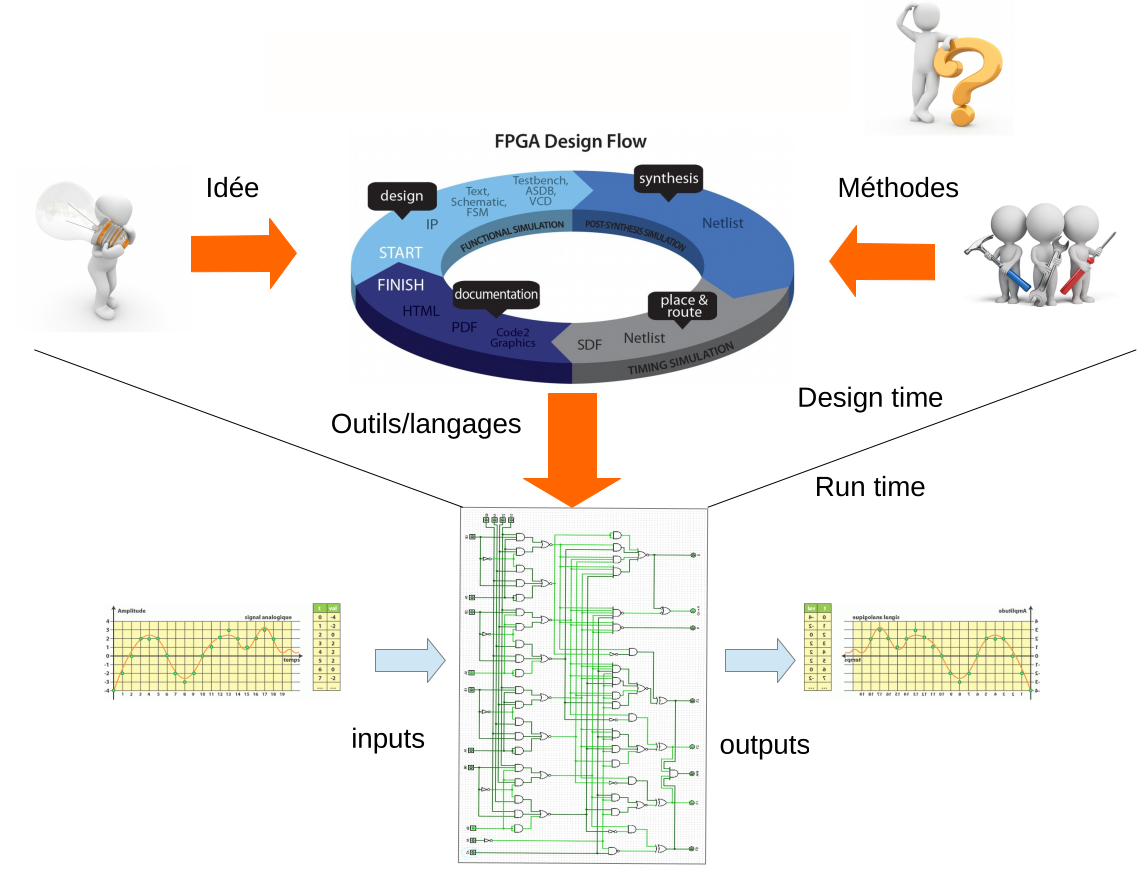
\includegraphics[scale=0.3]{./images/idee_circuit.png}
%         \end{column}
%     \end{columns}
% \end{frame}

%========================================================================================
% \begin{frame}{Equipe enseignante}
  \begin{columns}
    \begin{column}[T]{0.5\textwidth}
      \begin{itemize}
        \item Brest : \textbf{Jean-Christophe Le Lann}
        \begin{itemize}
          \item Enseignant-chercheur (Pr)
          \begin{itemize}
            \item ENSTA depuis 2009.
            \item Laboratoire LabSTICC UMR CNRS.
          \end{itemize}
          \item Ingénieur chez Thomson R\& D France
          \begin{itemize}
            \item 1999-2009 : conception des SoC de compression
          \end{itemize}
          \item Créateur et directeur technique startup
          \begin{itemize}
            \item Outils de CAO pour le codesign HW/SW.
          \end{itemize}
          \item Parcours :
          \begin{itemize}
            \item Habilitation à Diriger des Recherches.
            \item Thèse de doctorat d'Informatique.
            \item DEA de Microélectronique.
            \item Maîtrise de Physique fondamentale.
          \end{itemize}
        \end{itemize}
      \end{itemize}
    \end{column}
    \begin{column}[T]{0.5\textwidth}
      \begin{itemize}
        \item Référent Palaiseau : Pr. Omar Hammami
        \item Environ 12 intervenants
        \begin{itemize}
          \item Enseignant-cherheurs ENSTA
          \item Ingénieurs CEA
          \item Ingénieurs IN2P3
          \item Doctorants etc.
        \end{itemize}
      \end{itemize}
    \end{column}
  \end{columns}

  \begin{alertblock}{Remerciements}
    Support audio-visuel et pédagogique Brest-Palaiseau.
  \end{alertblock}
\end{frame}

\begin{frame}{Exemples de circuits et systèmes : broadcast vidéo}
  \begin{alertblock}{Société "Numérique"}
    \begin{itemize}
      \item usages, stockage...
      \item ...algorithmes et circuits complexes
    \end{itemize}
  \end{alertblock}
  \begin{center}
    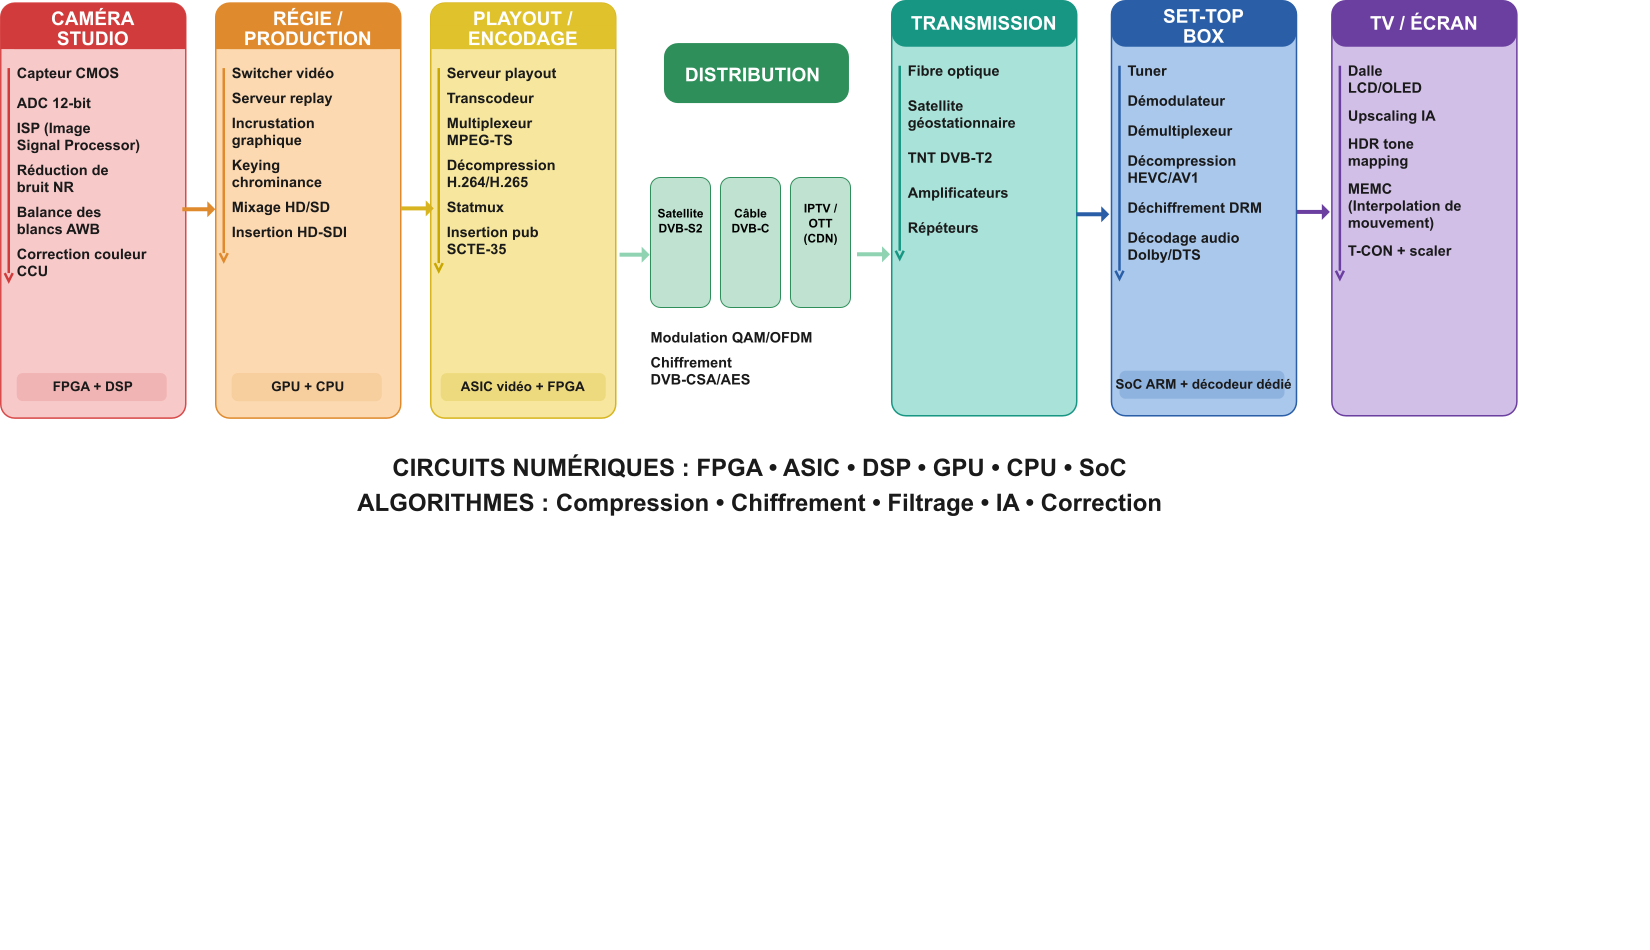
\includegraphics[width=\textwidth]{./images/chaine-diffusion-tv.png}
  \end{center}
\end{frame}

%
% \begin{frame}{De l'idée au circuit}
%   \begin{center}
%     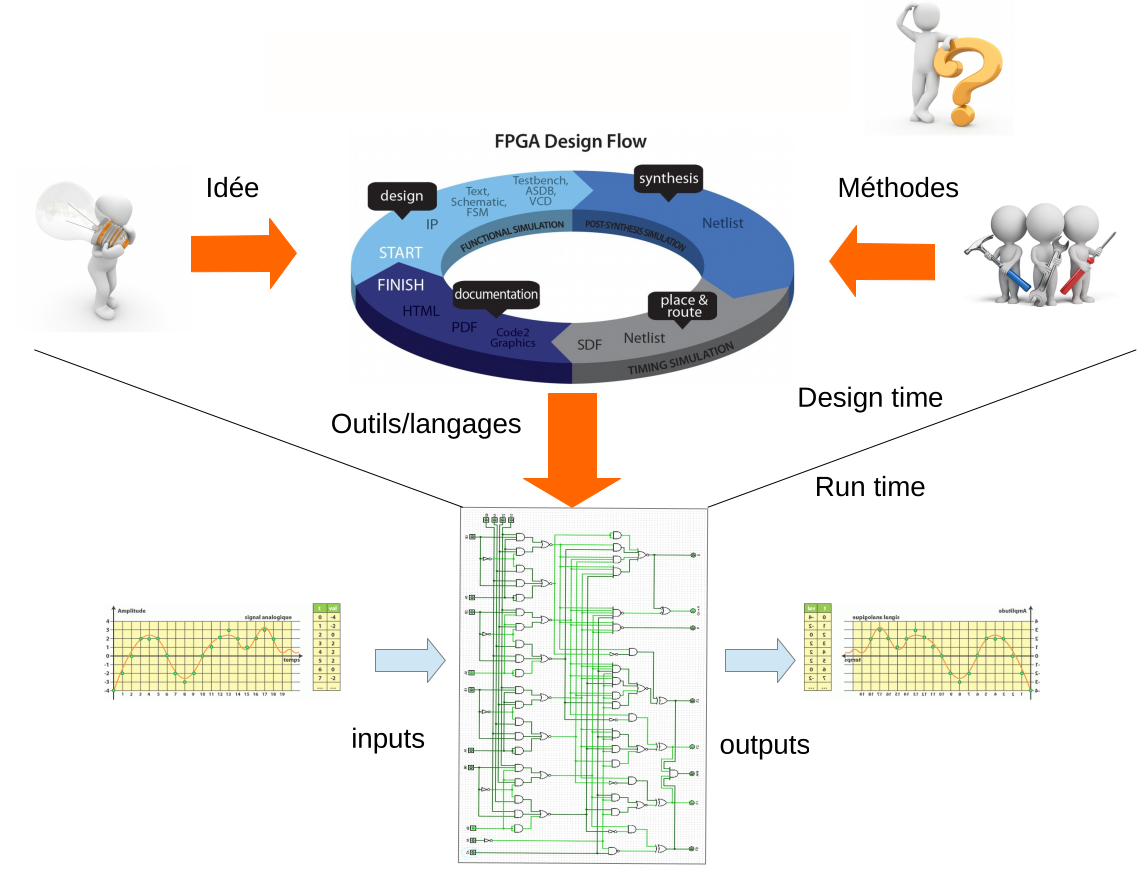
\includegraphics[scale=0.32]{./images/idee_circuit.png}
%   \end{center}
% \end{frame}
%
% \begin{frame}{Numérisation}
%   \begin{center}
%     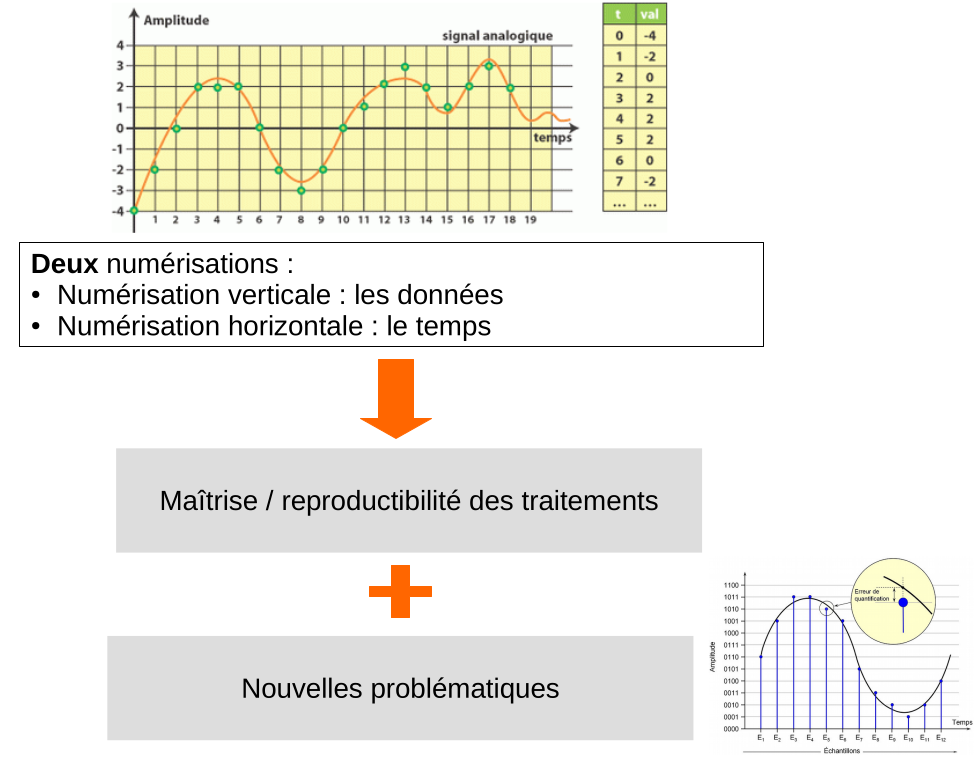
\includegraphics[scale=0.25]{./images/numerisation.png}
%   \end{center}
% \end{frame}
%
% %========================================================================================
% \begin{frame}{Plan}
%   \tableofcontents
% \end{frame}
%
% \begin{frame}{Objectifs}
%   \begin{columns}
%     \begin{column}{0.5\textwidth}
%       \begin{enumerate}
%         \item Comprendre les fondements de la conception des systèmes numériques :
%         \begin{itemize}
%           \item Logique booléenne : combinatoire et séquentielle.
%           \item Calcul sur silicium, chemin de données
%           \item Machines d'états finis : contrôleurs / automates
%           \item Principe des Micro-architectures
%           \item Initiation à VHDL au niveau logique et structurel
%         \end{itemize}
%
%         \item Premiers pas vers les systèmes embarqués :
%         \begin{itemize}
%           \item Processeurs, périphériques, communication
%         \end{itemize}
%       \end{enumerate}
%     \end{column}
%
%     \begin{column}{0.5\textwidth}
%       \begin{center}
%         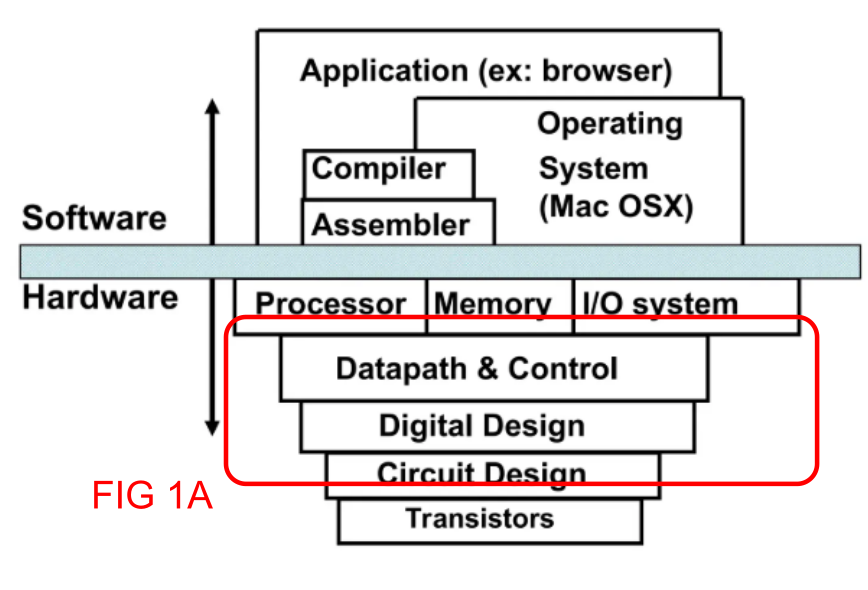
\includegraphics[scale=0.25]{./images/scope.png}
%       \end{center}
%     \end{column}
%   \end{columns}
%
%
% \end{frame}

% %========================================================================================
% \section{Physique des semi-conducteurs et micro-électronique : un aperçu}
% %========================================================================================
% \begin{frame}{Le Silicium : élément chimique}
  \begin{center}
    %\includesvg[scale=0.35]{images/silicium_atome}
    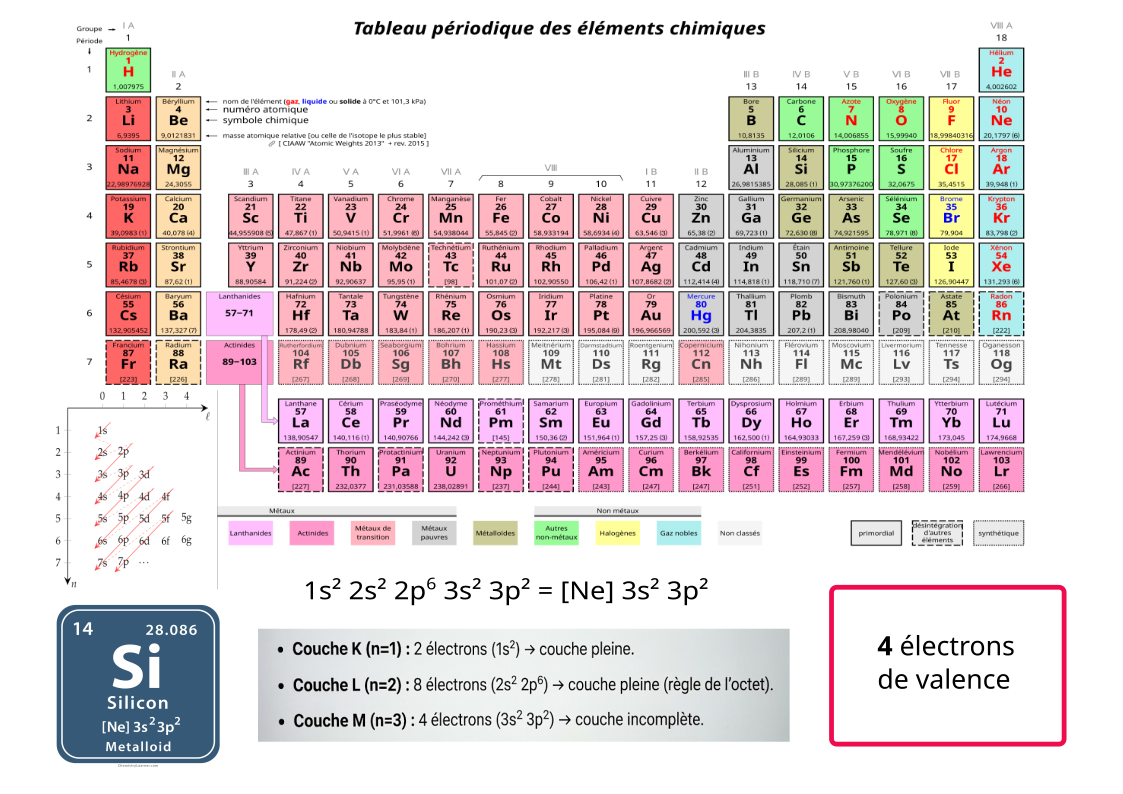
\includegraphics[scale=0.35]{images/silicium_atome.png}
  \end{center}
\end{frame}

\begin{frame}{Le Silicium : à partir de la Silice}
 \begin{enumerate}

   \item \textbf{Extraction} : réduction carbothermique de la silice
   \begin{itemize}
     \item Réaction chimique à 3000° : SiO2 + 2C → Si (liquide) + 2CO (gaz)
     \item Source de carbone : charbon, coke,...
     \item Pureté 98-99.5 \% insuffisante pour l'Electronique (silicium métallurgique MG-Si)
   \end{itemize}

   \item \textbf{Purification} : Procédé \textbf{Siemens}
   \begin{itemize}
     \item Hydrochloration du silicium métallurgique : trichlorosilane $SiHCl_3$ (gazeux)
     \item Si + 3 HCl → SiHCl3 + H2
     \item Distillation : chauffage à 1100°. Décomposition et obtention de "germes".
     \item Pureté 99.9999999\% (polycristallin) voire plus pour l'Electronique.
   \end{itemize}

   \item \textbf{Obtention d'un monocristal} : Procédé \textbf{Czokralski}
   \begin{itemize}
     \item Fusion et germination.
     \item Tirage et rotation.
     \item Formation du lingot.
   \end{itemize}

 \end{enumerate}
\end{frame}

\begin{frame}{Le Silicium : méthode Czokralski}
  \begin{center}
    \includesvg[scale=0.4]{images/silicium_czokralski}
  \end{center}
\end{frame}

% \begin{frame}{Le Silicium : cristallogaphie}
  \begin{center}
    %\includesvg[scale=0.35]{images/silicium_cristal}
    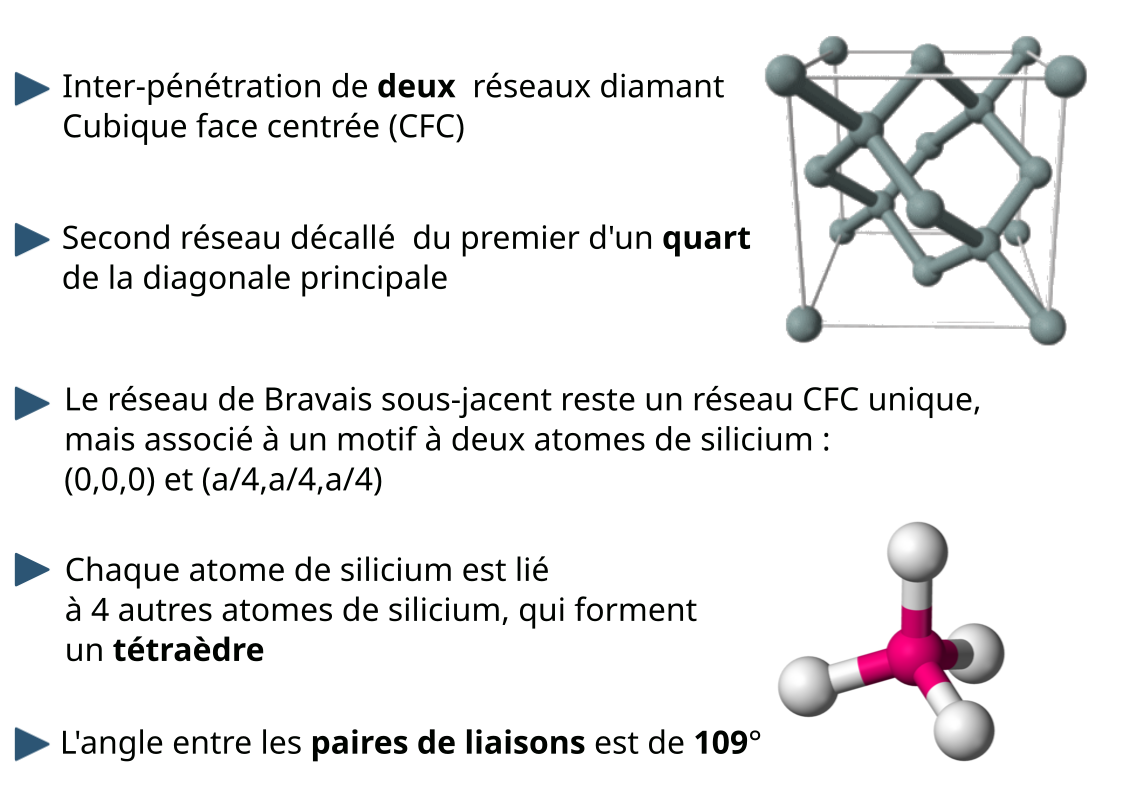
\includegraphics[scale=0.35]{images/silicium_cristal.png}
  \end{center}
\end{frame}

\begin{frame}{Le Silicium : cristallogaphie}
  \begin{center}
    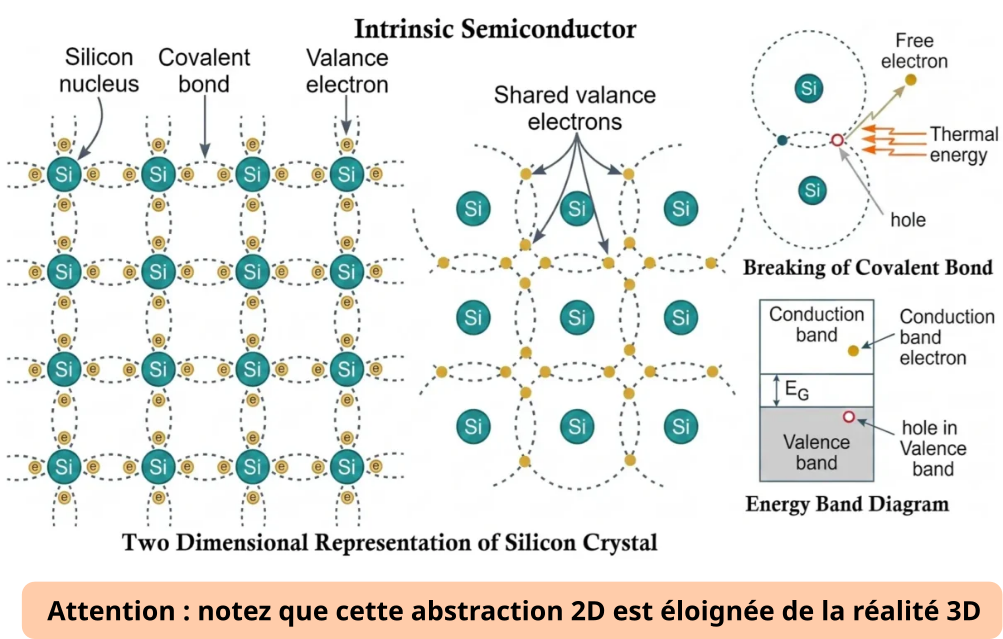
\includegraphics[scale=0.4]{images/silicium_thermal_energy.png}
  \end{center}
\end{frame}

\begin{frame}{Le Silicium : théorie des bandes}
  \begin{center}
    \includesvg[scale=0.38]{images/silicium_bandes.svg}
  \end{center}
\end{frame}

\begin{frame}{Le Silicium : dopage N et P}
  \begin{center}
    \includesvg[scale=0.35]{images/silicium_bore_antimoine.svg}
    %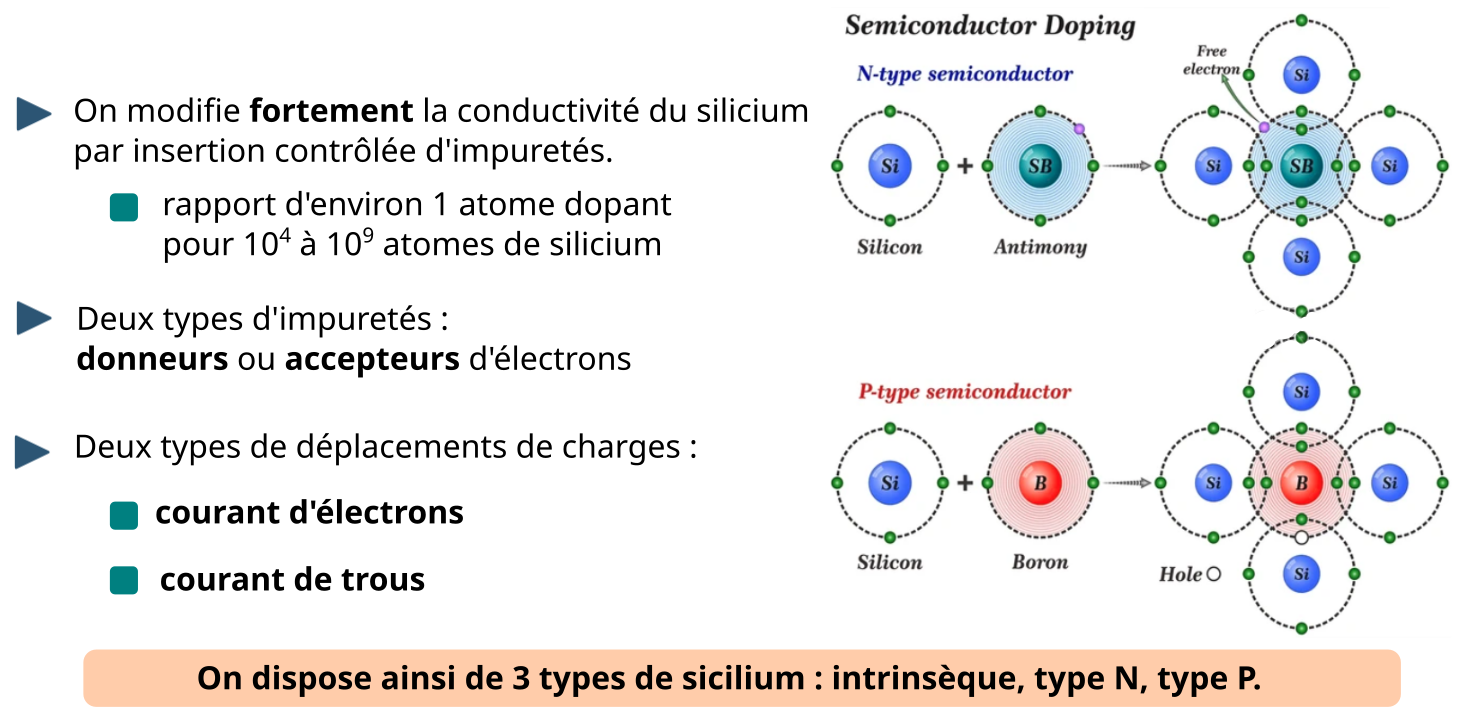
\includegraphics[scale=0.4]{images/silicium_bore_antimoine.png}
  \end{center}
\end{frame}

% \begin{frame}{Jonction P-N : mise en contact de deux types de silicium }

\begin{enumerate}
  \item Mise en contact et diffusion
  \begin{itemize}
    \item \textbf{Loi de Fick} : les porteurs majoritaires diffusent.
    \item Les électrons de N vers P, les trous de P vers N
    \item \textbf{Recombinaisons} au voisinage immédiat de l'interface.
  \end{itemize}
  \item La \textbf{zone de déplétion} (ZCE) : zone vidée de ses porteurs libres
  \begin{itemize}
    \item côté N : des ions donneurs positifs non compensés
    \item côté P : des ions accepteurs négatifs non compensés
    \item ZCE : région dépourvue de porteurs mobiles mais chargée électriquement.
  \end{itemize}

  \item \textbf{Champ interne} et barrière de potentiel
  \begin{itemize}
    \item un champ électrique interne $\vec{E}$, orienté de N vers P, qui s'oppose à la diffusion.
  \end{itemize}

  \item Équilibre dynamique :
  \begin{itemize}
    \item Une barrière de potentiel $V_0$ s'établit (environ 0,7 V pour le silicium).
    \item Le courant de diffusion (dû au gradient) équilibre exactement le courant de conduction (dû  au champ électrique).
    \item Le niveau de Fermi $E_F$ devient continu à travers tout le matériau.
  \end{itemize}
\end{enumerate}
\end{frame}

%\begin{frame}{Jonction P-N : polarisation }
%
% \begin{enumerate}
%   \item Polarisation directe
%   \begin{itemize}
%     \item + côté P, - côté N.
%     \begin{itemize}
%       \item La tension externe s'oppose au champ interne :
%       \item la barrière de potentiel diminue. la ZCE se rétrécit
%       \item la diffusion des majoritaires redevient dominante
%       \item le courant croît exponentiellement avec V.
%     \end{itemize}
%     \item Loi de Shockley : $I = I_0(e^{V/V_T} - 1)$
%   \end{itemize}
%   \item Polarisation inverse
%   \begin{itemize}
%     \item champ externe renforce le champ interne
%     \item la ZCE s'élargit
%     \item très faible courant
%   \end{itemize}
% \end{enumerate}
% \end{frame}

\begin{frame}{Jonction P-N : polarisation}
    \begin{columns}[T]  % [T] aligne en haut, [c] centré, [b] en bas
        \begin{column}{0.5\textwidth}  % Colonne de gauche (50% de la largeur)
          \begin{enumerate}
            \item Polarisation directe
            \begin{itemize}
              \item + côté P, - côté N.
              \begin{itemize}
                \item La tension externe s'oppose au champ interne.
                \item la barrière de potentiel diminue. la ZCE se rétrécit.
                \item la diffusion des majoritaires redevient dominante.
                \item le courant croît exponentiellement avec V.
              \end{itemize}
              \item Loi de Shockley : $I = I_0(e^{V/V_T} - 1)$
            \end{itemize}
            \item Polarisation inverse
            \begin{itemize}
              \item champ externe renforce le champ interne
              \item la ZCE s'élargit
              \item très faible courant
            \end{itemize}
          \end{enumerate}
        \end{column}

        \begin{column}{0.5\textwidth}  % Colonne de droite (50% de la largeur)
            \centering
            \includesvg[width=\textwidth, height=0.7\textheight, keepaspectratio]{./images/jonction_1}
            % ou avec des dimensions fixes :
            % \includesvg[width=5cm, height=5cm]{chemin/vers/votre_fichier}
        \end{column}
    \end{columns}
\end{frame}

\begin{frame}{Transistor bipolaire : structure}
  \begin{columns}[T]  % [T] aligne en haut, [c] centré, [b] en bas
        \begin{column}{0.45\textwidth}  % Colonne de gauche (50% de la largeur)
          \begin{itemize}
            \item Deux jonctions PN dos-à-dos : type NPN ou PNP
            \item Trois régions : émetteur, base, collecteur
            \item Base fine et faiblement dopée
            \item Jonction émetteur-base polarisée en direct
            \item Jonction base-collecteur polarisée en inverse
            \item Effet transistor : le courant de base contrôle le courant de collecteur
          \end{itemize}
        \end{column}

        \begin{column}{0.55\textwidth}  % Colonne de droite (50% de la largeur)
            \centering
            \includegraphics[scale=0.18]{./images/bipolar.jpg}
        \end{column}
    \end{columns}
\end{frame}

\begin{frame}{Transistor bipolaire : fonctionnement}
\begin{itemize}
    \item Gain en courant $\beta = I_C / I_B$ (typiquement 50 à 300)
    \item Régime actif : amplification (usage analogique)
    \item Régime saturé : interrupteur fermé (les 2 jonctions en direct)
    \item Régime bloqué : interrupteur ouvert (les 2 jonctions en inverse)
    \item Relation fondamentale : $I_E = I_B + I_C$
    \item Applications : amplification, commutation, logique TTL
\end{itemize}
\end{frame}
%
% \begin{frame}{Transistor bipolaire : fonctionnement}
%   \begin{itemize}
%   \item  \textbf{Injection} : La polarisation en direct de la jonction EB "pousse" les trous (porteurs majoritaires de l'émetteur P) à travers la jonction pour les injecter dans la base N.
%   \item \textbf{Traversée de la base} : Comme la base est très fine et faiblement dopée, la grande majorité des trous injectés ne trouvent pas d'électrons avec lesquels se recombiner. Ils diffusent donc à travers la base jusqu'à la jonction CB.
%   \item \textbf{Collecte} : La jonction CB étant polarisée en inverse, elle crée un champ électrique intense dans sa zone de déplétion. Ce champ "aspire" immédiatement les trous qui arrivent de la base et les accélère vers le collecteur P.
%   \item \textbf{Recombinaison} (Courant de base) : Une très petite fraction des trous (typiquement 1 \% à 5 \%) se recombine avec les électrons dans la base. Pour maintenir la neutralité électrique, le circuit de base doit fournir continuellement de nouveaux électrons, ce qui constitue le faible courant de base.
%   \end{itemize}
% \end{frame}

\begin{frame}{Transistors MOS (nmos)}
  \begin{columns}[c] % [T] aligne en haut, [c] centré, [b] en bas
    \begin{column}{0.5\textwidth}  % Colonne de gauche (50% de la largeur)
      \begin{itemize}
        \item Transistor à \textbf{effet de champ} (FET) à canal N, constitué d’un substrat P, de deux zones N+ (Source et Drain) et d’une grille isolée par un oxyde ($SiO_2$).
        \item Commande \textbf{par la tension} grille-source $V_{GS}$
        \item Création un canal conducteur (ou non) d’électrons entre Source et Drain.
        \item Inconvénient : un inverseur NMOS utilise une résistance de pull-up.
      \end{itemize}
    \end{column}

    \begin{column}{0.5\textwidth}  % Colonne de droite (50% de la largeur)
        \begin{center}
          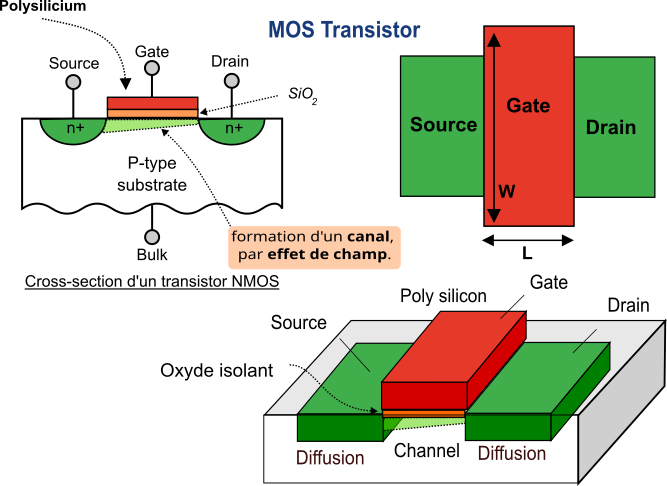
\includegraphics[scale=0.43]{./images/nmos_diagram.png}
        \end{center}
    \end{column}
    \end{columns}
\end{frame}



%===================================================

\begin{frame}{Le procédé de photolithographie}

\begin{columns}[T,onlytextwidth]

  % ---- Colonne de gauche : points clés ----
  \begin{column}{0.47\textwidth}
    \footnotesize
    \begin{itemize}\setlength{\itemsep}{3pt}
      \item \textbf{Principe} : transférer un motif géométrique d'un masque vers une résine photosensible déposée sur une plaquette (\emph{wafer})
      \item \textbf{Dépôt} : enduction centrifuge (\emph{spin coating}) d'un film uniforme
      \item \textbf{Insolation} : exposition UV à travers un masque optique portant le motif
      \item \textbf{Développement} : dissolution sélective des zones exposées (résine positive) ou non exposées (négative)
      \item \textbf{Gravure} : transfert du motif dans le substrat (voie humide ou plasma)
      \item \textbf{Retrait} de la résine (\emph{stripping})
      \item Résolution limitée par la diffraction $\Rightarrow$ UV profond, immersion, EUV
    \end{itemize}
  \end{column}

  % ---- Colonne de droite : schéma ----
  \begin{column}{0.51\textwidth}
    \centering
    \includegraphics[width=\textwidth]{./images/photolitho_v2.pdf}
  \end{column}

\end{columns}

\end{frame}


\begin{frame}{ASML : le leader de la photo-lithographie}
  \begin{columns}
    \begin{column}{0.7\textwidth}
      \begin{center}
        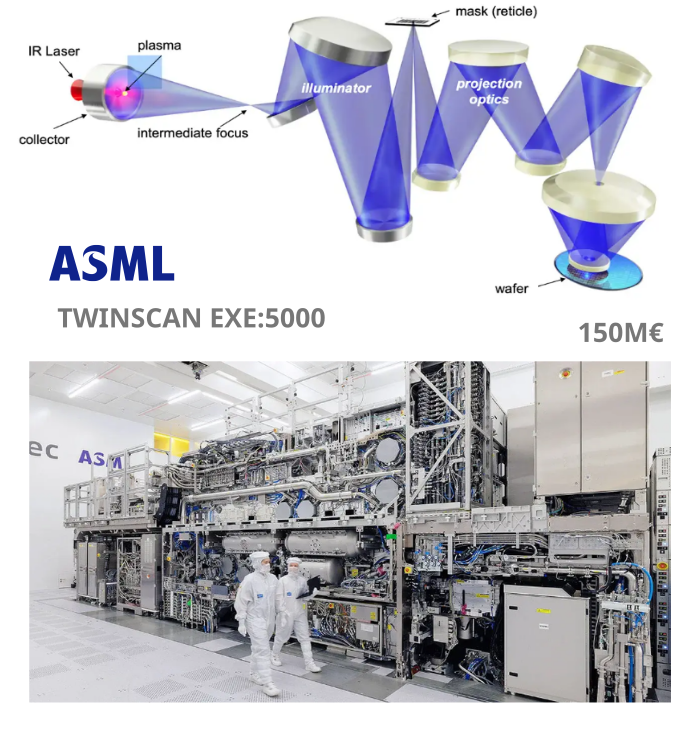
\includegraphics[scale=0.37]{./images/asml.png}
      \end{center}
    \end{column}
    \begin{column}{0.3\textwidth}
      \begin{center}
        \includegraphics[scale=0.4]{./images/ic_3d.jpg}
      \end{center}
    \end{column}
  \end{columns}
\end{frame}

% \section{Technologie CMOS : Complementary Metal Oxyde Semiconductor}

\begin{frame}{CMOS --- Transistors CMOS }
  \begin{columns}
    \begin{column}{0.5\textwidth}  % Colonne de droite (50% de la largeur)
      \begin{alertblock}{Paradigme dominant}
        Fondement de la microélectronique numérique actuelle
      \end{alertblock}
      \begin{itemize}
        \item Association de transistors \textbf{NMOS} et \textbf{PMOS} sur un même substrat.
        \item NMOS : conduit lorsque la grille est à $V_{DD}$
        \item PMOS : conduit lorsque la grille est à $0\,$V
        \begin{itemize}
          \item Se substitue à la résistance de pull-up du NMOS.
          \item Montage \textbf{dual} : série $\rightleftarrows$ parallèle.
        \end{itemize}
        \item Effet de champ : la \textbf{tension} de grille contrôle le canal.
        \item Isolation par \textbf{oxyde de grille} $\Rightarrow$ haute impédance d'entrée.
      \end{itemize}
    \end{column}

    \begin{column}{0.5\textwidth}  % Colonne de droite (50% de la largeur)
        \begin{center}
          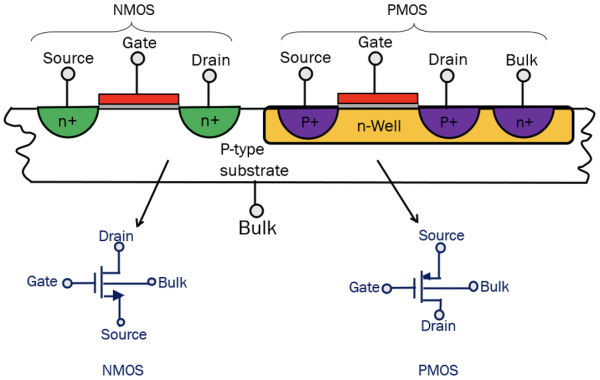
\includegraphics[scale=0.45]{./images/cmos_0.png}
        \end{center}
    \end{column}
  \end{columns}
\end{frame}

\begin{frame}{Le modèle de Schichman--Hodges : caractéristiques $I_D(V_{DS})$}

\begin{alertblock}{Physique}
 Caractérisation du comportement \textit{analogique} du MOS.
\end{alertblock}

\begin{columns}[T,totalwidth=\textwidth]

% ---------- Colonne de gauche : équations ----------
\begin{column}{0.48\textwidth}

\footnotesize
\textbf{1. Blocage} \quad ($V_{GS} - V_T \leq 0$)
\[
I_D = 0
\]

\vspace{1mm}
\textbf{2. Zone linéaire} \quad ($0 < V_{DS} < V_{GS}-V_T$)
\[
I_D = k_n \tfrac{W}{L}\!\left[(V_{GS}\!-\!V_T)V_{DS} - \tfrac{V_{DS}^2}{2}\right]\!\left(1+\lambda V_{DS}\right)
\]

\vspace{1mm}
\textbf{3. Saturation} \quad ($V_{DS} \geq V_{GS}-V_T$)
\[
I_D = \frac{k_n}{2} \frac{W}{L}(V_{GS}-V_T)^2\left(1+\lambda V_{DS}\right)
\]

\vspace{2mm}
\scriptsize
$k_n=\mu_n C_{ox}$ (transconductance) $\;\cdot\;$ $V_T$ (seuil) $\;\cdot\;$ $\lambda$ (modulation de canal) $\;\cdot\;$ $W/L$ (géométrie)

\vspace{2mm}
\footnotesize
\alert{Un seul jeu d'équations décrit tout le comportement}, du blocage à la saturation.

\end{column}

% ---------- Colonne de droite : courbes caractéristiques ----------
\begin{column}{0.52\textwidth}
  \begin{center}
    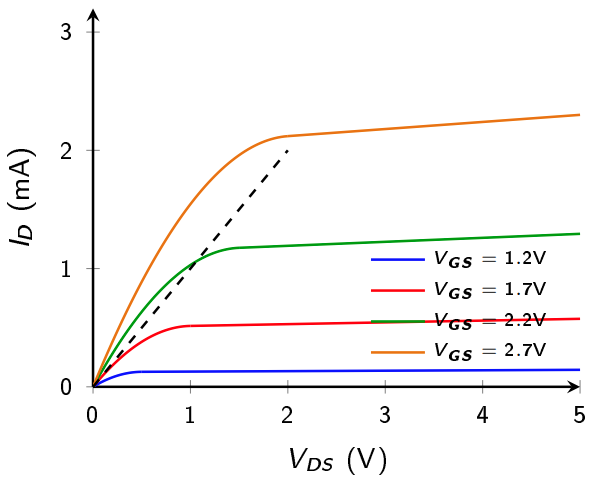
\includegraphics[scale=0.3]{./images/caract_mos.png}
  \end{center}
\end{column}

\end{columns}

\end{frame}

% \begin{frame}{Le transistor comme interrupteur commandé}
  \begin{columns}
    \begin{column}{0.5\textwidth}
      \textbf{Transistor NMOS}
      \begin{itemize}
        \item Conduit (interrupteur fermé) si \textbf{Grille = 1}
        \item Bloqué si Grille = 0
        \item \fbox{Transmet bien un \textbf{0} logique}
      \end{itemize}
      \vspace{0.5cm}
      \textbf{Transistor PMOS}
      \begin{itemize}
        \item Conduit (interrupteur fermé) si \textbf{Grille = 0}
        \item Bloqué si Grille = 1
        \item \fbox{Transmet bien un \textbf{1} logique}
      \end{itemize}
    \end{column}
    \begin{column}{0.5\textwidth}
      \centering
      \begin{circuitikz}[scale=1.0]
        \draw (0,0) node[nmos, anchor=D](M1){};
        \draw (M1.G) node[left=0.3cm]{$G$};
        \draw (M1.S) node[below=0.2cm]{$S$};
        \draw (M1.D) node[above=0.2cm]{$D$};
      \end{circuitikz}
      \hspace{0.5cm}
      \begin{circuitikz}[scale=1.0]
        \draw (0,0) node[pmos, anchor=D](M2){};
        \draw (M2.G) node[left=0.3cm]{$G$};
        \draw (M2.S) node[above=0.2cm]{$S$};
        \draw (M2.D) node[below=0.2cm]{$D$};
      \end{circuitikz}
    \end{column}
  \end{columns}
\end{frame}
%
\begin{frame}{Table de fonctionnement simplifiée}
  \centering
  \begin{tabular}{ccc}
    \toprule
    Entrée grille & NMOS & PMOS \\
    \midrule
    0 & bloqué & passant \\
    1 & passant & bloqué \\
    \bottomrule
  \end{tabular}
  \vspace{0.5cm}

  \begin{block}{Idée fondatrice du CMOS}
    On associe systématiquement un réseau de NMOS (relié à la masse)
    et un réseau de PMOS \emph{dual} (relié à l'alimentation $V_{DD}$)
    pour qu'à chaque instant \textbf{un seul} des deux réseaux conduise.
  \end{block}
\end{frame}
%
% ------------------------------------------------------------
%\section{L'inverseur CMOS}

\begin{frame}{L'inverseur CMOS : la porte de base}
  \begin{columns}
    \begin{column}{0.35\textwidth}
      \begin{circuitikz}[scale=1.1, transform shape]
        % --- Alimentation ---
        \draw (0,4.6) node[above]{$V_{DD}$};
        \draw (0,4.6) to[short] (0,4.1);
        % --- PMOS ---
        \draw (0,4.1) node[pmos, anchor=S](P1){};
        % --- Noeud de sortie Y ---
        \draw (P1.D) to[short] (0,2.6);
        \draw (0,2.6) to[short] (0.7,2.6) node[right]{$Y$};
        % --- NMOS ---
        \draw (0,2.6) node[nmos, anchor=D](N1){};
        % --- Connexion des grilles ---
        \draw (P1.G) -- ++(-0.8,0) coordinate(pgate);
        \draw (N1.G) -- ++(-0.8,0) coordinate(ngate);
        \draw (pgate) -- (ngate);
        % --- Entrée A alignée avec Y ---
        \coordinate (aPoint) at (pgate |- N1.D);
        \draw (aPoint) -- ++(-0.5,0) node[left]{$A$};
        % --- Masse ---
        \draw (N1.S) to[short] (0,1.1);
        \draw (0,1.1) node[ground]{};
      \end{circuitikz}
    \end{column}
    \begin{column}{0.65\textwidth}
      \begin{itemize}
        \item Entrée $A$ commune aux deux grilles
        \item PMOS en haut (côté $V_{DD}$)
        \item NMOS en bas (côté masse)
        \item Si $A=0$ : PMOS passant, NMOS bloqué $\Rightarrow Y=1$
        \item Si $A=1$ : PMOS bloqué, NMOS passant $\Rightarrow Y=0$
      \end{itemize}
      \vspace{0.3cm}
      \[ Y = \overline{A} \]
    \end{column}
  \end{columns}
\end{frame}

\begin{frame}{L'inverseur CMOS : chronogramme}
  \begin{center}
    %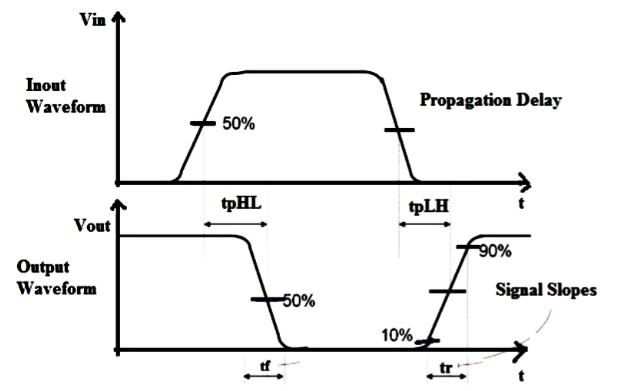
\includegraphics[scale=0.5]{./images/inverter_slopes.png}
    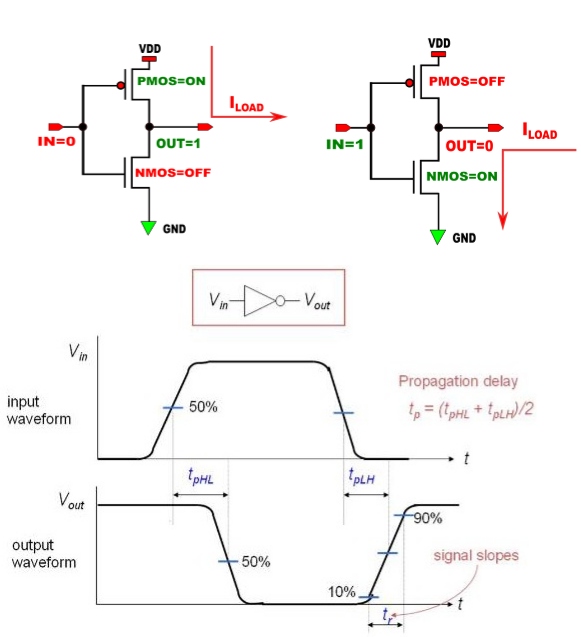
\includegraphics[scale=0.45]{./images/inverter.png}
  \end{center}
\end{frame}

\begin{frame}{Porte NAND à 2 entrées : montage dual}
  \begin{columns}
    \begin{column}{0.35\textwidth}
      \begin{circuitikz}[scale=1.0, transform shape]
        % --- Rail VDD ---
        \draw (-1.6,6.0) node[above]{$V_{DD}$} to[short] (2.2,6.0);

        % --- PMOS A (gauche) ---
        \draw (-0.8,6.0) to[short] (-0.8,5.6);
        \node[pmos, anchor=S] (Pa) at (-0.8,5.6) {};
        \draw (Pa.G) -- ++(-0.3,0) node[left]{$A$};

        % --- PMOS B (droite) ---
        \draw (1.4,6.0) to[short] (1.4,5.6);
        \node[pmos, anchor=S] (Pb) at (1.4,5.6) {};
        \draw (Pb.G) -- ++(-0.3,0) node[left]{$B$};

        % --- Jonction des deux drains PMOS (en parallele) ---
        \draw (Pa.D) -- (-0.8,4.3) -- (0.3,4.3);
        \draw (Pb.D) -- (1.4,4.3) -- (0.3,4.3);
        \draw (0.3,4.3) -- (0.3,3.6);

        % --- Noeud de sortie Y, sorti sur le cote pour eviter le chevauchement ---
        \draw (0.3,3.6) to[short] (1.6,3.6) node[right]{$Y$};
        \filldraw (0.3,3.6) circle (0.05);

        % --- NMOS A (haut de la pile) ---
        \node[nmos, anchor=D] (Na) at (0.3,3.6) {};
        \draw (Na.G) -- ++(-0.9,0) node[left]{$A$};

        % --- NMOS B (bas de la pile), en serie avec Na ---
        \node[nmos, anchor=D] (Nb) at (0.3,2.3) {};
        \draw (Na.S) -- (Nb.D);
        \draw (Nb.G) -- ++(-0.9,0) node[left]{$B$};

        % --- Masse ---
        \draw (Nb.S) -- (0.3,1.0) node[ground]{};
      \end{circuitikz}
    \end{column}
    \begin{column}{0.65\textwidth}
      \begin{itemize}
        \item NMOS $A$ et $B$ en \textbf{série} $\to$ conduit
          seulement si $A=1$ ET $B=1$
        \item PMOS $A$ et $B$ en \textbf{parallèle} (dual)
        \item $Y=0$ uniquement si $A=B=1$
      \end{itemize}
      \[ Y = \overline{A \cdot B} \]
    \end{column}
  \end{columns}
\end{frame}

\begin{frame}{Pourquoi ça marche : jamais de court-circuit}
  \begin{itemize}
    \item En régime statique, un seul chemin conducteur existe entre
      $V_{DD}$ et $Y$, ou entre $Y$ et la masse — jamais les deux.
    \item Conséquence : \textbf{pas de consommation statique}
      (hors fuites), contrairement aux logiques NMOS seules
      (résistance de charge) ou bipolaires.
    \item La consommation du CMOS est essentiellement
      \textbf{dynamique} : elle a lieu lors des commutations
      (charge/décharge des capacités de sortie).
  \end{itemize}
\end{frame}

\begin{frame}{Dualité N-P en CMOS : autre exemple}
  \begin{center}
    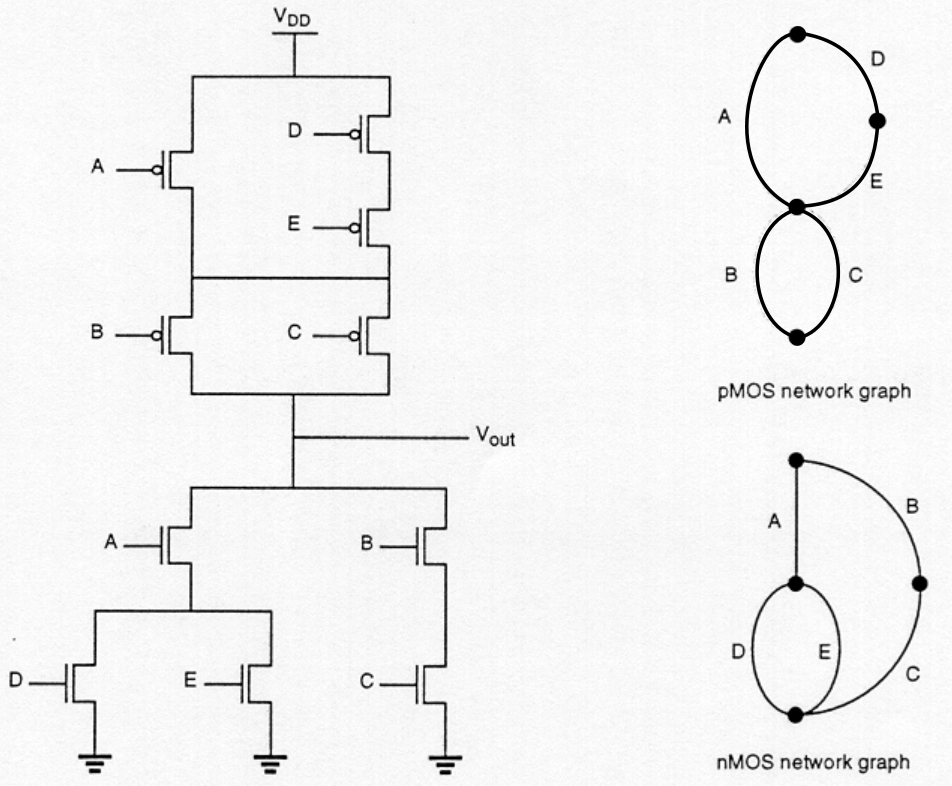
\includegraphics[scale=0.35]{./images/dualite_eulerien.png}
  \end{center}
\end{frame}

% % ------------------------------------------------------------
% \section{Porte NAND}
%
% \begin{frame}{Porte NAND à 2 entrées}
%   \begin{columns}
%     \begin{column}{0.55\textwidth}
%       \begin{circuitikz}[scale=1.0, transform shape]
%         % --- Rail VDD ---
%         \draw (-0.8,5.2) node[above]{$V_{DD}$};
%         \draw (-0.8,5.2) to[short] (1.4,5.2);
%         % --- PMOS A (gauche) et PMOS B (droite), en parallele ---
%         \draw (-0.8,5.2) to[short] (-0.8,4.7);
%         \draw (-0.8,4.7) node[pmos, anchor=S](Pa){};
%         \draw (Pa.G) -- ++(-0.8,0) node[left]{$A$};
%         \draw (1.4,5.2) to[short] (1.4,4.7);
%         \draw (1.4,4.7) node[pmos, anchor=S](Pb){};
%         \draw (Pb.G) -- ++(0.8,0) node[right]{$B$};
%         % --- jonction des deux drains PMOS vers Y ---
%         \draw (Pa.D) to[short] (-0.8,3.8) to[short] (0.3,3.8);
%         \draw (Pb.D) to[short] (1.4,3.8) to[short] (0.3,3.8);
%         \draw (0.3,3.8) to[short] (0.3,3.2);
%         \draw (1.1,3.2) node{$Y$};
%         % --- NMOS A et B en serie ---
%         \draw (0.3,3.2) node[nmos, anchor=D](Na){};
%         \draw (Na.G) -- ++(-0.8,0) node[left]{$A$};
%         \draw (Na.S) to[short] (0.3,1.9);
%         \draw (0.3,1.9) node[nmos, anchor=D](Nb){};
%         \draw (Nb.G) -- ++(-0.8,0) node[left]{$B$};
%         \draw (Nb.S) to[short] (0.3,0.9);
%         \draw (0.3,0.9) node[ground]{};
%       \end{circuitikz}
%     \end{column}
%     \begin{column}{0.45\textwidth}
%       \begin{itemize}
%         \item NMOS $A$ et $B$ en \textbf{série} $\to$ conduit
%           seulement si $A=1$ ET $B=1$
%         \item PMOS $A$ et $B$ en \textbf{parallèle} (dual)
%         \item $Y=0$ uniquement si $A=B=1$
%       \end{itemize}
%       \[ Y = \overline{A \cdot B} \]
%     \end{column}
%   \end{columns}
% \end{frame}


%========================================================================================
%\section{Montée en abstraction}
%========================================================================================
% 
\begin{frame}{Conception des Portes logiques : plusieurs niveaux d'abstraction}
  [Guyot TIMA 1995]
  \begin{center}
    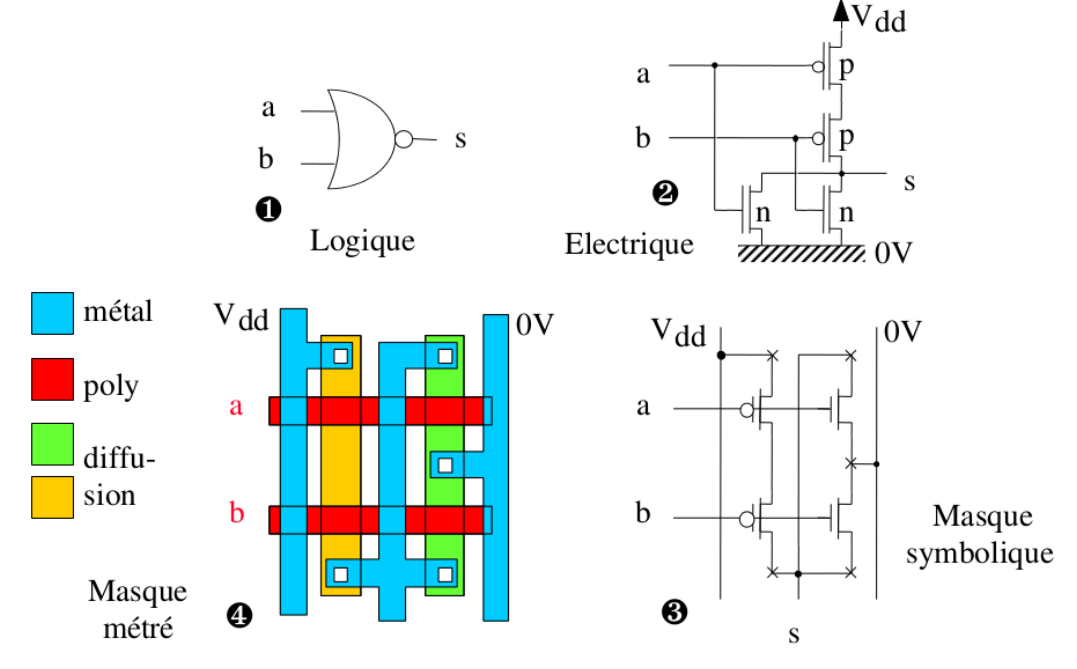
\includegraphics[scale=0.3]{./images/guyot.png}
  \end{center}
\end{frame}


\begin{frame}{Conception des Systèmes numériques : Y de Gajski}

  \begin{columns}[T,onlytextwidth]
    \begin{column}{0.47\textwidth}
      \begin{center}
        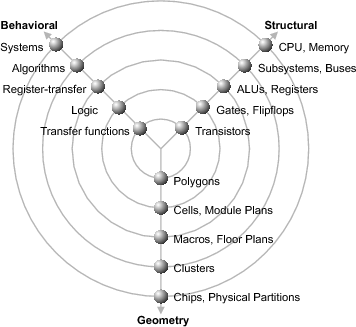
\includegraphics[scale=0.4]{./images/y_gajski.png}
        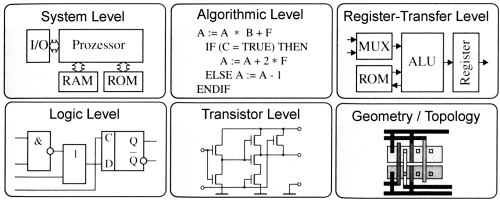
\includegraphics[scale=0.3]{./images/y_gajski_2.png}
      \end{center}
    \end{column}

    \begin{column}{0.51\textwidth}
      \begin{center}
        \includegraphics[scale=0.15]{./images/gajski.jpg}
        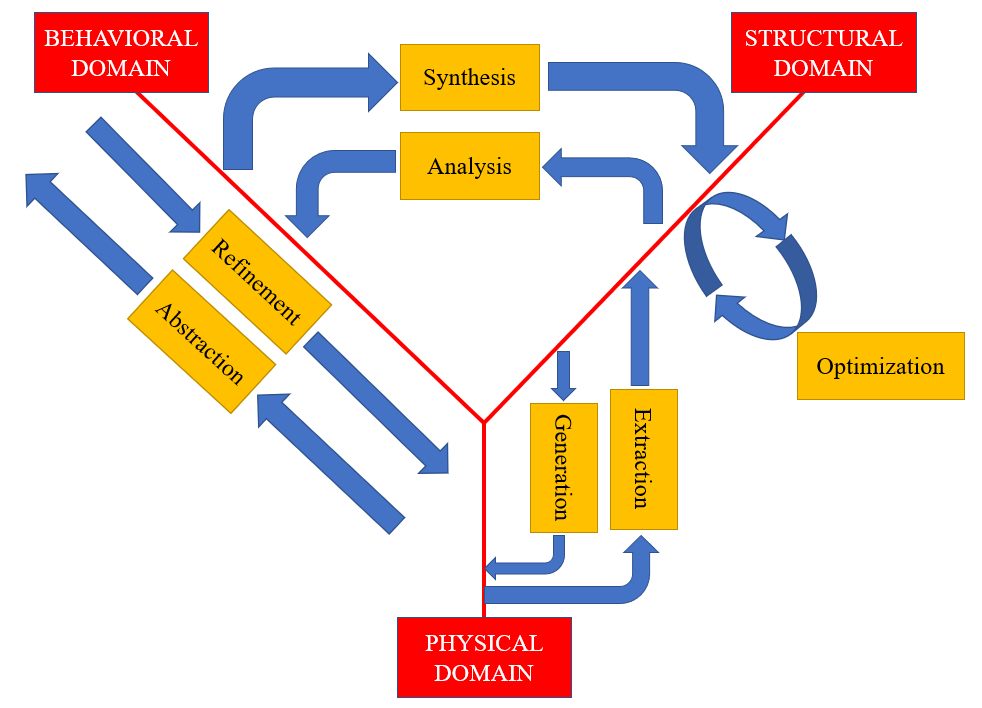
\includegraphics[scale=0.30]{./images/y_gajski_3.png}
      \end{center}
    \end{column}
  \end{columns}

\end{frame}

\begin{frame}{Abstraction et Synthèse automatique}
  \begin{columns}
    \begin{column}{0.50\textwidth}
      \begin{itemize}
        \item Complexité des systèmes
        \item Recours à des langages spécifiques : HDL.
        \begin{itemize}
          \item Description
          \item Simulation (laboratoire virtuel)
          \item Synthèse automatique
        \end{itemize}
        \item ...à différents niveaux d'abstraction.
      \end{itemize}
    \end{column}
    \begin{column}{0.50\textwidth}
      \begin{center}
        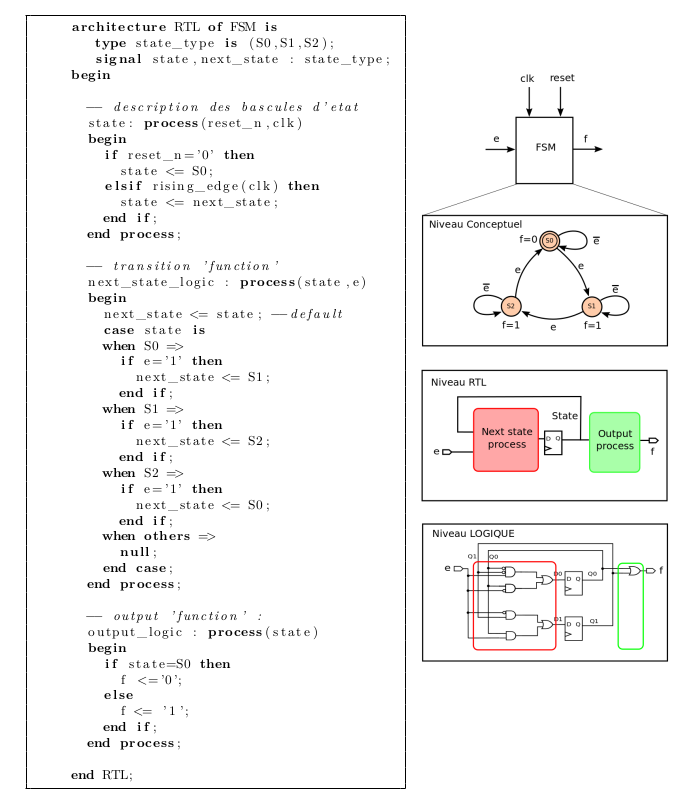
\includegraphics[scale=0.25]{./images/fsm.png}
      \end{center}
    \end{column}
  \end{columns}
\end{frame}

\begin{frame}{Abstractions : système et automates}
  \begin{center}
    \includegraphics[scale=1.0]{./images/gemini_abstraction_soc.jpeg}
  \end{center}
\end{frame}

% \begin{frame}{Electronic Design Automation (EDA) : }

  \begin{columns}[T]

    \begin{column}{0.52\textwidth}
      \begin{itemize}
        \setlength{\itemsep}{4pt}
        \item \textbf{Spécification système} : besoins et fonctionnalités
        \item \textbf{Conception architecturale} : partitionnement HW/SW
        \item \textbf{Conception fonctionnelle et RTL} : description HDL (Verilog/VHDL)
        \item \textbf{Synthèse logique} : RTL $\rightarrow$ netlist de portes
        \item \textbf{Conception physique} : placement et routage
        \item \textbf{Vérification physique et signoff} : DRC, LVS, STA
        \item \textbf{Fabrication} : gravure sur wafer (silicium)
        \item \textbf{Packaging et test} : mise en boîtier, tests
        \item \textbf{Puce finale} : circuit intégré prêt à l'emploi
      \end{itemize}
    \end{column}


    \begin{column}{0.44\textwidth}
      \centering
      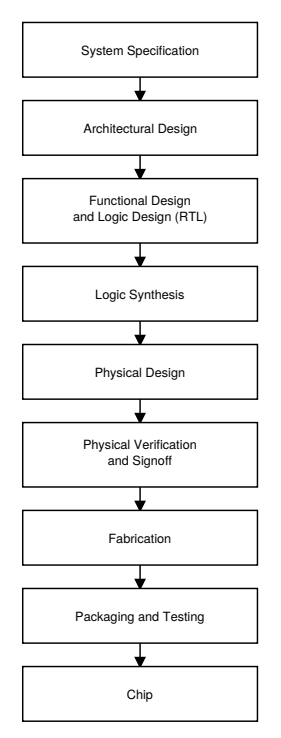
\includegraphics[width=\textwidth,height=0.85\textheight,keepaspectratio]{./images/eda_flow.png}
      %\includesvg[width=\textwidth,height=0.85\textheight,keepaspectratio]{./images/eda_flow.svg}
    \end{column}

  \end{columns}
\end{frame}

% \begin{frame}{Du transistor (1947) au \texttt{xeon} d'Intel}
    \begin{center}
        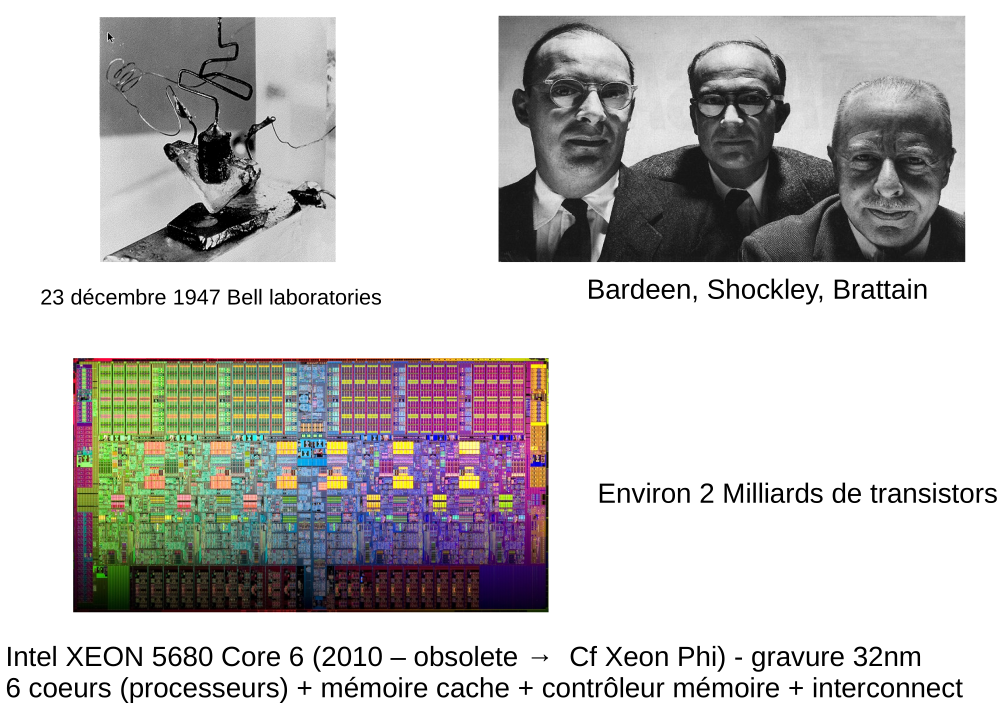
\includegraphics[scale=0.3]{./images/transistor_1947.png}
    \end{center}
\end{frame}

\begin{frame}{Jalons historiques: loi de Moore}
  \begin{columns}[T] % [T] aligne en haut, [c] centré, [b] en bas
    \begin{column}{0.5\textwidth}  % Colonne de gauche (50% de la largeur)
      \begin{itemize}
        \item Doublement du nombre de transistors tous les 18 mois.
      \end{itemize}
      \begin{center}
        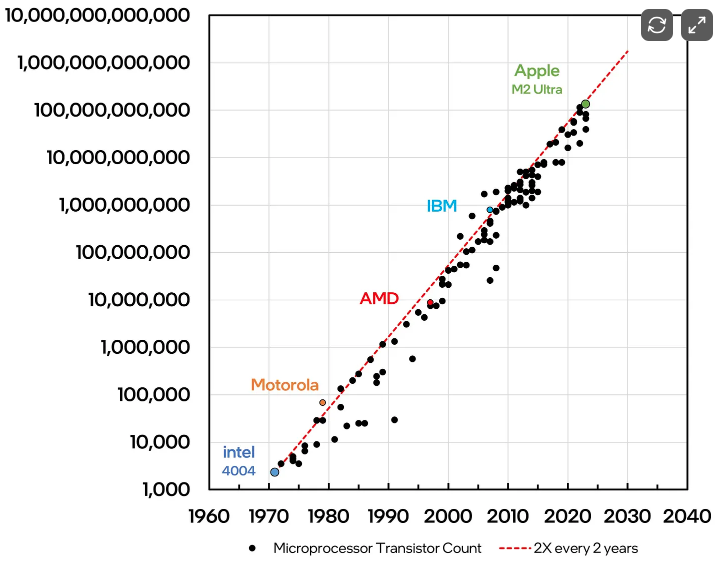
\includegraphics[scale=0.3]{./images/history_moore.png}
      \end{center}
    \end{column}

    \begin{column}{0.5\textwidth}  % Colonne de droite (50% de la largeur)
        \begin{itemize}
        \item Perspective historique plus large.
        \end{itemize}
        \begin{center}
          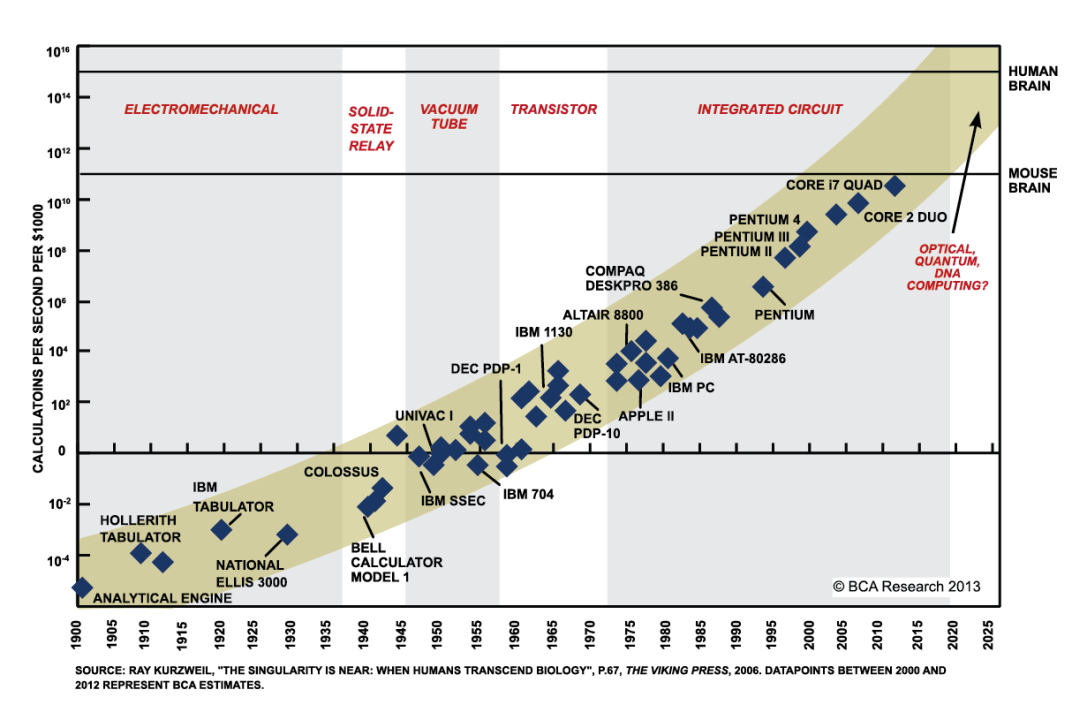
\includegraphics[scale=0.20]{./images/history_1.png}
        \end{center}
        1971 : Intel 4004
    \end{column}
    \end{columns}
\end{frame}

\begin{frame}{Le cas des mémoires :}
    \begin{center}
        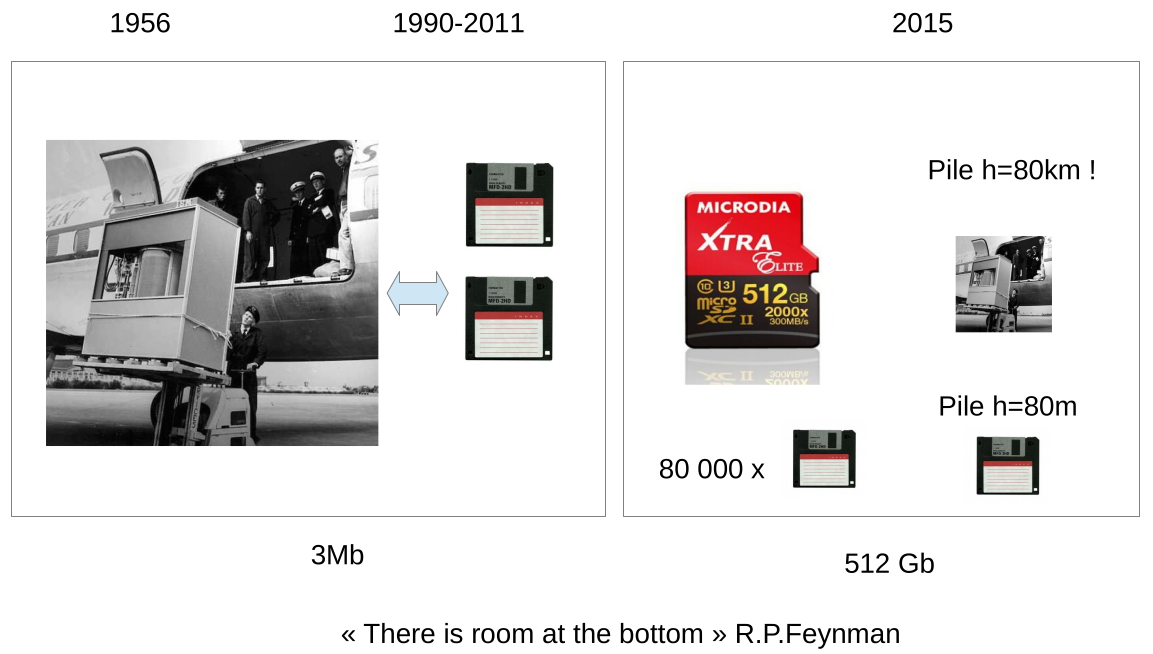
\includegraphics[scale=0.3]{./images/disquette.png}
    \end{center}
\end{frame}


%================================================%\begin{frame}{Base de numération}
  \begin{itemize}
    \item On parle de \textit{base} ou \textit{radix} $r$.
    \begin{itemize}
      \item Utilisation des \textit{symboles} de $0$ à $r-1$.
      \item Notation \textit{positionnelle}
      \item Les entiers se décomposent à l'aide des coefficients des puissances de $r$.
    \end{itemize}

    \item Base 10 :
    \begin{itemize}
      \item $142 = 1\times 10^2 + 4 \times 10^1 + 2  \times 10^0$
    \end{itemize}

    \item Base 10, nombres décimaux :
    \begin{itemize}
      \item $142.34 = 1\times 10^2 + 4 \times 10^1 + 2  \times 10^0 + 3 \times 10^{-1} + 4 \times 10^{-2}$
      \item Nombre décimal $\frac{a}{10^n}$ $\rightarrow$ nombre fini de symboles.
      \item Attention : tous les nombres à virgule ne sont pas décimaux !
      \item Attention : lorsqu'on change de base, le nombre de coefficients nécessaires, pour une précision donnée, varie.
      \begin{itemize}
        \item Exemple : $0.2$ ne se représente pas avec un nombre fini de \texttt{bits} dans la base $2$ !
      \end{itemize}

    \end{itemize}
  \end{itemize}
\end{frame}

\begin{frame}{Notations non positionnelles : trois exemples}

\textbf{Chiffres romains} \hfill \textit{(additif, symboles à valeur fixe)}

\smallskip
I = 1, V = 5, X = 10, L = 50, C = 100, D = 500, M = 1000

\smallskip
Exemple : MCMXCIV = 1000 + (1000-100) + (100-10) + (5-1) = \textbf{1994}

\vspace{0.6cm}

\textbf{Système unaire} \hfill \textit{(additif pur, une marque par unité)}

\smallskip
\texttt{|||||} = 5 \qquad \texttt{|||||||} = 7 \quad \textit{(ou groupes de 5)}

\vspace{0.6cm}

\textbf{Hiéroglyphes égyptiens} \hfill \textit{(additif, un symbole par puissance de 10)}

\smallskip
\begin{tabular}{ll}
$\vert$ = 1 & $\cap$ = 10 \\
$\curlywedge$ = 100 & $\odot$ = 1000 \\
\end{tabular}

\smallskip
24 s'écrit : deux « anses » + quatre « traits » --- \textbf{l'ordre n'importe pas}

\vspace{0.4cm}

\centering
\footnotesize\itshape
Dans tous ces systèmes, la position d'un symbole ne modifie jamais sa valeur.

\end{frame}

\begin{frame}{Généralisation}
  La formule générale pour la base 10 est bien entendu :
  $$ x = \sum_{i=-\infty}^{i=+\infty} c_i.10^i, c_i \in \{0,\dots,9 \}$$
  et se généralise :
  $$ \forall r, x = \sum_{i=-\infty}^{i=+\infty} c_{i,r}.r^i, c_{i,r} \in \{0,\dots,(r-1)\}$$
  Lors des changements de base, il faut une notation pour préciser la base de représentation.
  \begin{itemize}
    \item Par exemple : $ 142_{10} = 10001110_{2}$
    \item En logiciel : $ 142_{10} = \text{\texttt{0b10001110}} = \text{\texttt{0x8e}} = \text{\texttt{0o216}}$

    \end{itemize}
\end{frame}

\begin{frame}{Compter en binaire : convertir par table}

  \begin{columns}
    \begin{column}{0.5\textwidth}
      \begin{table}[h]
        \centering
        \resizebox{!}{0.44\textheight}{%
        \begin{tabular}{c|ccccc}
          \toprule
          \multirow{2}{*}{\textbf{Decimal count}} & \multicolumn{5}{c}{\textbf{Binary count}} \\
          \cmidrule(l){2-6} & \textbf{16s} & \textbf{8s} & \textbf{4s} & \textbf{2s} & \textbf{1s} \\
          \midrule
          0  &   &   &   &   & 0 \\
          1  &   &   &   &   & 1 \\
          2  &   &   &   & 1 & 0 \\
          3  &   &   &   & 1 & 1 \\
          4  &   &   & 1 & 0 & 0 \\
          5  &   &   & 1 & 0 & 1 \\
          6  &   &   & 1 & 1 & 0 \\
          7  &   &   & 1 & 1 & 1 \\
          8  &   & 1 & 0 & 0 & 0 \\
          9  &   & 1 & 0 & 0 & 1 \\
          10 &   & 1 & 0 & 1 & 0 \\
          11 &   & 1 & 0 & 1 & 1 \\
          12 &   & 1 & 1 & 0 & 0 \\
          13 &   & 1 & 1 & 0 & 1 \\
          14 &   & 1 & 1 & 1 & 0 \\
          15 &   & 1 & 1 & 1 & 1 \\
          16 & 1 & 0 & 0 & 0 & 0 \\
          17 & 1 & 0 & 0 & 0 & 1 \\
          18 & 1 & 0 & 0 & 1 & 0 \\
          19 & 1 & 0 & 0 & 1 & 1 \\
          \midrule
          & $2^4$ & $2^3$ & $2^2$ & $2^1$ & $2^0$ \\
          \cmidrule(l){2-6}
          & \multicolumn{5}{c}{Powers of 2} \\
          \bottomrule
        \end{tabular}
        % \vspace{1pt}
        % \hspace{2.cm}\textbf{MSB} \hfill \textbf{LSB}\hspace{0.1cm}
        } %resizex
      \end{table}
    \end{column}

    \begin{column}{0.5\textwidth}
      \begin{table}[h]
      \centering
        \resizebox{!}{0.44\textheight}{
        \begin{tabular}{cccc}
        \toprule
        \textbf{Décimal} & \textbf{Binaire} & \textbf{Octal} & \textbf{Hexadécimal} \\
        \midrule
        0  & 0000 & 0  & 0 \\
        1  & 0001 & 1  & 1 \\
        2  & 0010 & 2  & 2 \\
        3  & 0011 & 3  & 3 \\
        4  & 0100 & 4  & 4 \\
        5  & 0101 & 5  & 5 \\
        6  & 0110 & 6  & 6 \\
        7  & 0111 & 7  & 7 \\
        8  & 1000 & 10 & 8 \\
        9  & 1001 & 11 & 9 \\
        10 & 1010 & 12 & A \\
        11 & 1011 & 13 & B \\
        12 & 1100 & 14 & C \\
        13 & 1101 & 15 & D \\
        14 & 1110 & 16 & E \\
        15 & 1111 & 17 & F \\
        \bottomrule
      \end{tabular}
      }
      \end{table}
    \end{column}

  \end{columns}
\end{frame}

\begin{frame}{A quoi ça sert ?}
  \begin{center}
    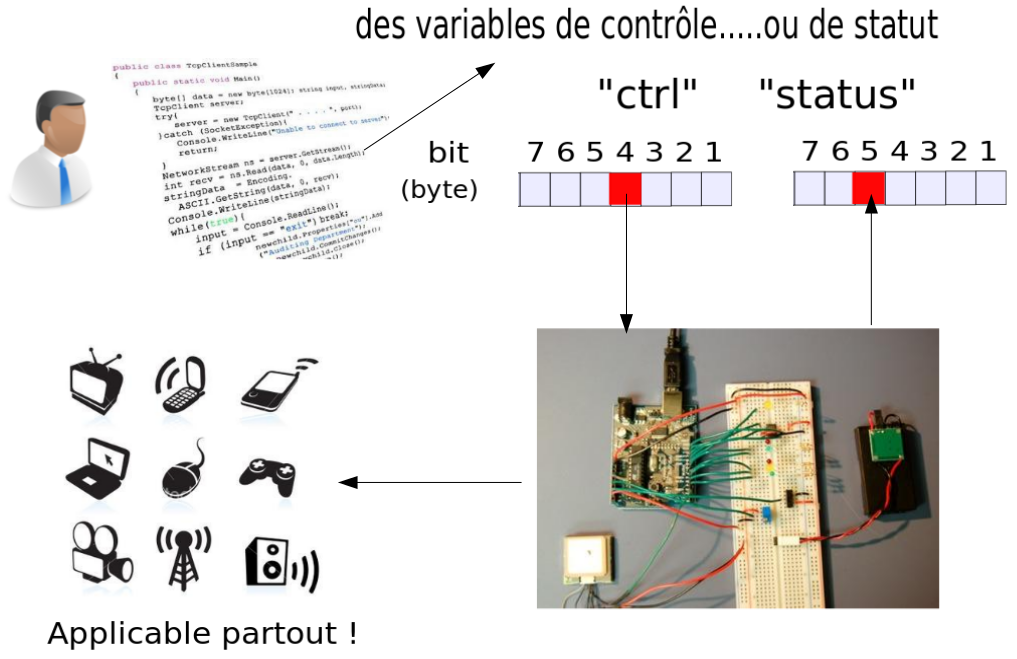
\includegraphics[scale=0.3]{./images/numbers_2.png}
  \end{center}
\end{frame}

\begin{frame}{A quoi ça sert ?}
  \begin{columns}
    \begin{column}{0.5\textwidth}
      \begin{center}
        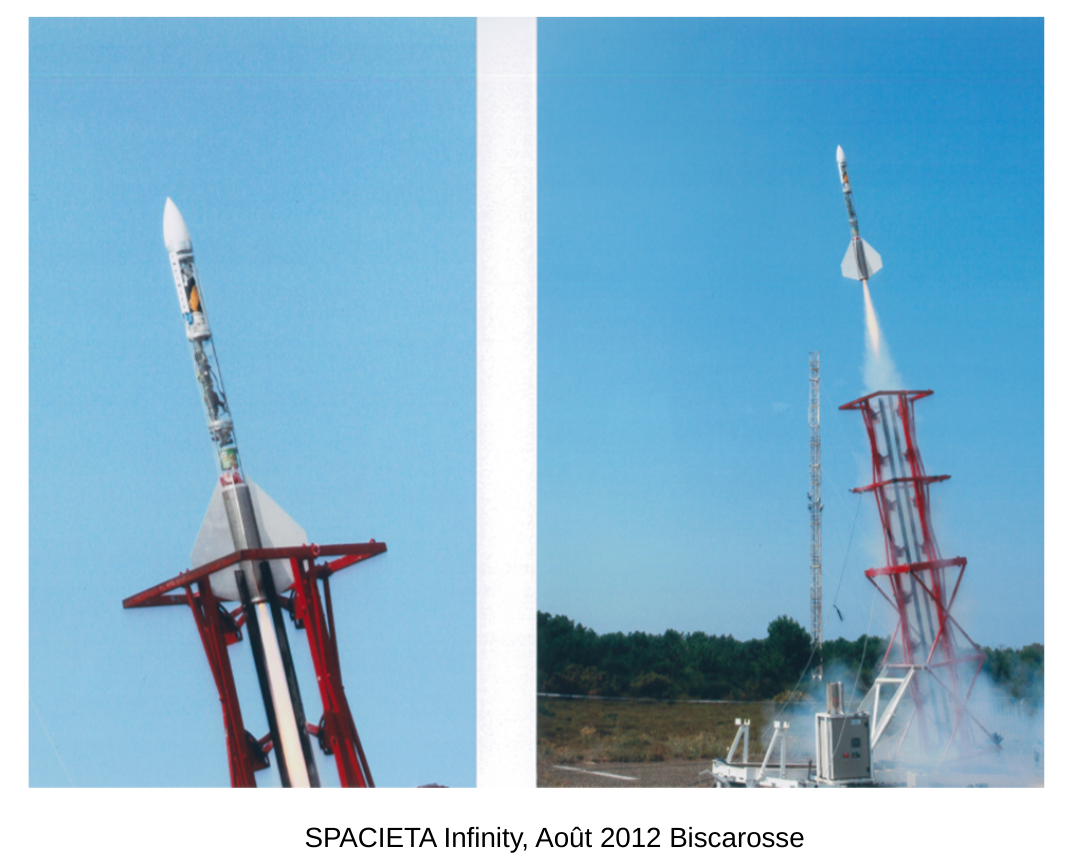
\includegraphics[scale=0.18]{./images/spacieta.png}
      \end{center}
    \end{column}

    \begin{column}{0.5\textwidth}
      \begin{center}
        \includegraphics[scale=0.18]{/home/jcll/Dropbox/IMAGES_TECHNIQUES/JOG.jpg}
      \end{center}
      JOG : conçu  à l'ENSTA Bretagne pour l'enseignement 1A.
    \end{column}
  \end{columns}
\end{frame}

\begin{frame}{Conversions entre bases : par table}
  \begin{center}
    \small $101101_{2} = \text{10\_1101}_{2} = \text{0010\_1101}_{2} = 2D_{16} = \mathbf{0x2D}$
  \end{center}

  \smallskip
  {\small Dans le cas de nombres fractionnaires, on rajoute des 0 à droite de la
  partie fractionnaire. Ainsi~:}

  \begin{center}
    \small le nombre $1011.01_{2} = \text{1011.0100}_{2} = B.4_{16}$
  \end{center}

  \smallskip
  {\small On procède de même pour la traduction octale.}

  \begin{center}
    \small $(10110001101011.1111)_{2} = (\text{101 110 001 101 011}.\text{111 100})_{2} = (36153.74)_{8}$
  \end{center}

  \smallskip
  \begin{center}
    \small
    \begin{tabular}{cccc}
      4 & 7 & . & F \quad E \\[-2pt]
      $\downarrow$ & $\downarrow$ & & $\downarrow$ \qquad $\downarrow$ \\[-2pt]
      0100 & 0111 & . & 1111 \quad 1110
    \end{tabular}

    \smallskip
    \small $47.\text{FE}_{16} \approx 1000111.1111111_{2}$
  \end{center}

\end{frame}

\begin{frame}{Conversions entre bases : par calcul}
  \begin{center}
    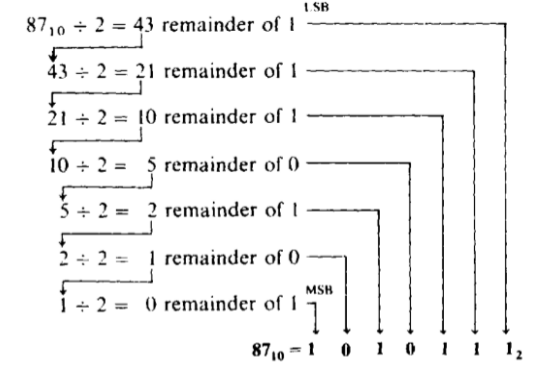
\includegraphics[scale=0.5]{./images/numbers_5.png}
  \end{center}
\end{frame}

\begin{frame}{Conversions entre bases : par calcul}
  \begin{center}
    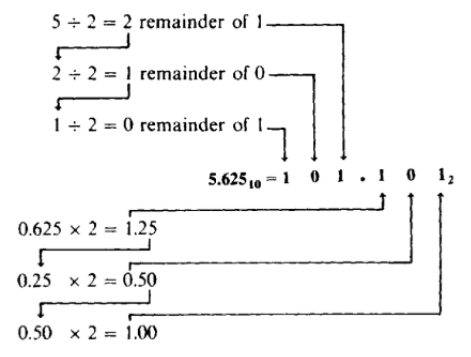
\includegraphics[scale=0.5]{./images/numbers_6.png}
  \end{center}
\end{frame}

\begin{frame}{Conversions entre bases : par calcul}
  \begin{center}
    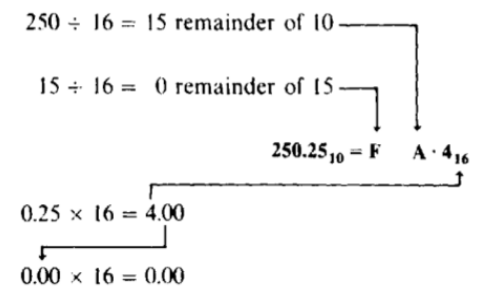
\includegraphics[scale=0.5]{./images/numbers_7.png}
  \end{center}
\end{frame}

\begin{frame}{Autres codes binaires : BCD décimal codé binaire}
  \begin{center}
    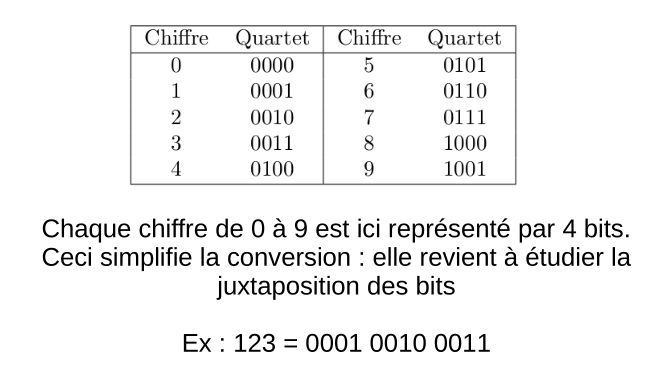
\includegraphics[scale=0.5]{./images/numbers_8.png}
  \end{center}
\end{frame}

\begin{frame}{Autres codes binaires : code de gray ou binaire réfléchi}
  \begin{center}
    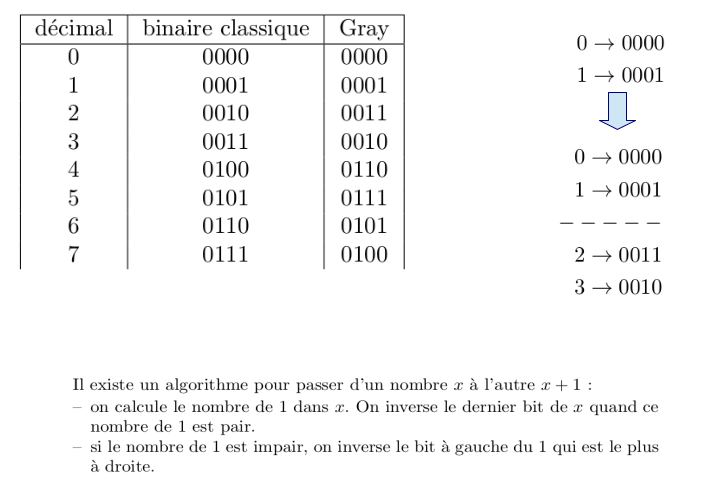
\includegraphics[scale=0.4]{./images/numbers_9.png}
  \end{center}
\end{frame}

\begin{frame}{Entiers positifs ou \texttt{unsigned}}
  \bigskip
  Soit un nombre $W$ de bits et soit $\vec{x} = [x_{w-1},x_{w-2},\ldots,x_0]$ de
  bits. Nous avons vu précédemment (sans la nommer) que la simple fonction~:
  \[
    B2U_w(\vec{x}) \doteq \sum_{i=0}^{w-1} x_i 2^i
  \]
  définit la valeur non-signée ("unsigned") de $\vec{x}$, dans $\mathbb{N}$.
  Les valeurs limites de cette fonction sont~:
  \[
    \begin{cases}
      UMax_w = \sum_{i=0}^{w-1} 2^i = 2^w - 1 \\
      UMmin_w = \sum_{i=0}^{w-1} 0 = 0
    \end{cases}
  \]
  On a donc~:
  \[
    B2U_w : \{0,1\}^w \to \{0,\ldots,2^w-1\}
  \]
\end{frame}

\begin{frame}{Complément à 2 sur w bits}
 \medskip
  \small
  De manière similaire, on définit désormais la fonction qui permet de
  calculer la valeur du vecteur $\vec{x}$ dans le cas d'une valeur signée,
  c'est-à-dire négative ou positive, \textbf{en complément à 2}.
  \[
    B2T_w(\vec{x}) \doteq -x_{w-1}2^{w-1} + \sum_{i=0}^{w-2} x_i 2^i
  \]
  Désormais, le bit de poids fort, le plus à gauche, contribue de manière
  négative à la somme totale. Précisons également que le 'T' vient de
  "two's complement". Calculons les valeurs min et max de cette fonction.
  Pour $\vec{x} = [10\ldots0]$ et $\vec{x} = [01\ldots1]$ respectivement, on
  trouve~:
  \[
    \begin{cases}
      TMin_w = -2^{w-1} \\
      TMax_w = \displaystyle\sum_{i=0}^{w-2} 2^i = 2^{w-1} - 1
    \end{cases}
  \]
  On a donc~:
  \[
    B2U_w : \{0,1\}^w \to \{-2^{w-1},\ldots,2^{w-1}-1\}
  \]
  On pourra également dénoter cette fonction $C_{2,w}(\vec{x})$.
\end{frame}

% ===================================================================
\begin{frame}{Complément à 2 sur w bits}

  \bigskip
  \begin{center}
    \renewcommand{\arraystretch}{1.15}
    \begin{tabular}{|c|c||c|}
      \hline
      \textbf{signé} & \textbf{bit vector} & \textbf{non-signé} \\
      \hline
      $-4$ & 100 & 4 \\ \hline
      $-3$ & 101 & 5 \\ \hline
      $-2$ & 110 & 6 \\ \hline
      $-1$ & 111 & 7 \\ \hline
      $0$  & 000 & 0 \\ \hline
      $1$  & 001 & 1 \\ \hline
      $2$  & 010 & 2 \\ \hline
      $3$  & 011 & 3 \\ \hline
    \end{tabular}
  \end{center}
\end{frame}

% ===================================================================
\begin{frame}{Nombres négatifs}

  \bigskip
  Le complément à 1 d'un nombre binaire consiste à simplement inverser tous
  ses bits.
  \medskip
  Le complément à 2 d'un nombre binaire s'obtient ainsi:
  \begin{itemize}
    \item On parcourt le nombre en partant de la droite (bit de poids faible).
    \item On recopie tel quel tous les bits tant qu'on n'a pas rencontré le premier 1.
    \item On recopie ce premier 1.
    \item On inverse tous les bits suivants (à gauche de ce 1).
  \end{itemize}
  Il existe toutefois une autre méthode, qui se retient plus facilement
  (peut-être). Elle consiste en une formule simple~:

  \bigskip
  \begin{columns}
    \begin{column}{0.35\textwidth}
      \colorbox{blue!20}{\parbox{0.9\textwidth}{\small\textbf{Attention~!!!!}\\
      $-134$ nécessite 9 bits et non 8}}
    \end{column}
    \begin{column}{0.65\textwidth}
      \begin{tikzpicture}
        \node[draw, fill=gray!30, minimum width=3cm, minimum height=1cm, font=\Large] (box) {$-X = \overline{X} + 1$};
        \node[below=0.9cm of box, align=left, xshift=0.3cm] (lab) {\footnotesize Addition classique\\\footnotesize (et non « OU » binaire)};
        \draw[-{Latex[length=3mm]}] (lab.north -| box.south) -- (box.south);
      \end{tikzpicture}
    \end{column}
  \end{columns}
\end{frame}

% ===================================================================
\begin{frame}{Nombres négatifs : représentations obsolètes}
  \bigskip
  \small
  La représentation en magnitude signée est simplement~:
  \[
    B2S_w(\vec{x}) \doteq (-1)^{x_{w-1}} \sum_{i=0}^{w-2} x_i 2^i
  \]
  Il existe également une représentation des nombres en complément à 1,
  très légèrement différente du complément à 2.
  \[
    B2T_w(\vec{x}) \doteq -x_{w-1}(2^{w-1}-1) + \sum_{i=0}^{w-2} x_i 2^i
  \]

  \bigskip
  \begin{center}
    \begin{tikzpicture}
      %\node[arrow, fill=red, minimum height=1cm, arrow head extend=2mm] (arr) {};
      \node[draw, fill=blue!10, align=center] {Ces représentations proposent 2 encodages pour 0~!};
    \end{tikzpicture}
  \end{center}

  \normalsize
  Dans le cas de la magnitude signée~:\\
  $+0 = 0\ldots.0$ et $-0 = 10\ldots0$
\end{frame}

% ===================================================================
\begin{frame}{Nombres négatifs : résumé}
  \begin{columns}[t]
    \begin{column}{0.42\textwidth}
      \tiny
      \renewcommand{\arraystretch}{1.05}
      \begin{tabular}{|c|c|}
        \hline
        \textbf{Signed decimal} & \textbf{8-bit 2's compl.} \\
        \hline
        $+127$ & 0111 1111 \\
        $+126$ & 0111 1110 \\
        $+125$ & 0111 1101 \\
        $\vdots$ & $\vdots$ \\
        $+1$ & 0000 0001 \\
        $+0$ & 0000 0000 \\
        \hline
        $-1$ & 1111 1111 \\
        $-2$ & 1111 1110 \\
        $\vdots$ & $\vdots$ \\
        $-125$ & 1000 0011 \\
        $-126$ & 1000 0010 \\
        $-127$ & 1000 0001 \\
        $-128$ & 1000 0000 \\
        \hline
      \end{tabular}
    \end{column}
    \begin{column}{0.58\textwidth}
      \small
      \begin{center}
        \begin{tikzpicture}
          \node[draw, fill=gray!30, minimum width=2.5cm, minimum height=0.9cm, font=\large] {$-X = \overline{X} + 1$};
        \end{tikzpicture}
      \end{center}

      \bigskip
      \colorbox{orange!40}{
      \begin{minipage}{0.95\textwidth}
        $-125\; ? =$

        \medskip
        $125 \quad = \quad 111\,1101$

        \medskip
        $/125 \quad = \quad \textcolor{red}{1}\,000\,0010$

        \medskip
        $/125+1 = 1\,000\,0011$
      \end{minipage}}
    \end{column}
  \end{columns}

  \bigskip
  \small
  Noter que les nombres en complément à 2 sont négatifs s'ils présentent un
  MSB à 1~!\\
  125 se représente sur 7 bits, mais pas $-125$~: il faut 8 bits
\end{frame}

% ===================================================================
\begin{frame}{\LARGE Exemple~: $-3$ sur 3 bits}


  \begin{columns}[t]
    \begin{column}{0.62\textwidth}
      \begin{itemize}
        \item $3_{10} = 011_2$
        \item $-3_{10} = /3_{10} + 1 = 100_2 + 1 = 101_2 = 5_{10}$~????
        \begin{itemize}
          \item 5 ne peut pas être représenté sur 3 bits, si on y
            représente également les nombres négatifs.
        \end{itemize}
      \end{itemize}

      \bigskip
      \colorbox{blue!30}{\parbox{0.95\textwidth}{\centering
        Pour un nombre donné de bits,\\
        il faut s'entendre sur le fait\\
        que la représentation d'un nombre est signée ou non}}
    \end{column}
    \begin{column}{0.35\textwidth}
      \small
      \begin{tabular}{cc}
        $+3$ & 011 \\
        $+2$ & 010 \\
        $+1$ & 001 \\
        $+0$ & 000 \\
        $-1$ & 111 \\
        $-2$ & 110 \\
        $-3$ & 101 \\
        $-4$ & 100 \\
      \end{tabular}
    \end{column}
  \end{columns}
\end{frame}

% ===================================================================
\begin{frame}{Addition et soustraction}

  \bigskip
  \textbf{Addition}~: classique
  \hfill
  \begin{minipage}{0.55\textwidth}
    \centering
    \renewcommand{\arraystretch}{1.2}
    \begin{tabular}{|l|r|}
      \hline
      & \textbf{Addition} \\
      \hline
      calcul & \begin{tabular}{r}0110\\ $+$0011\end{tabular} \\
      \hline
      retenus & 11 \\
      \hline
      résultat & 1001 \\
      \hline
    \end{tabular}
  \end{minipage}

  \bigskip
  \textbf{Soustraction : x - y}

  \small
  \begin{enumerate}
    \item on additionne $x$ et le complément à 2 de $y$
    \item si le résultat présente une retenue finale, on l'oublie~!
    \item s'il n'y a pas de retenue finale, on prend le complément à 2 du
      résultat et on place un signe "-" devant le nombre.
  \end{enumerate}

  \medskip
  \textbf{exemple}~: $x = 1101100_2$ et $y = 1011011_2$
  \[
    1101100 + 0100101 = 1\,0010001
  \]
  Le résultat est donc $x - y = 0010001_2$

  \hfill\tiny 108-91
\end{frame}

% ===================================================================
\begin{frame}{\LARGE Nombre en virgule fixe : ou \textit{fixed point}}

  \bigskip
  \begin{itemize}
    \item Déjà vu précédemment\ldots
    \item Le calculateur numérique devra connaître la position de la
      virgule, fixée une bonne fois pour toute.
    \item Impact sur les opérations classiques~:
    \begin{itemize}
      \item Le résultat de l'addition hérite de la position de la virgule
        identique à celle dans les opérandes
      \item Cela est changé pour les autres opérations.
    \end{itemize}
  \end{itemize}
\end{frame}

% ===================================================================
\begin{frame}{Nombres en virgule flottante : norme \texttt{ieee754}}

  \begin{center}
    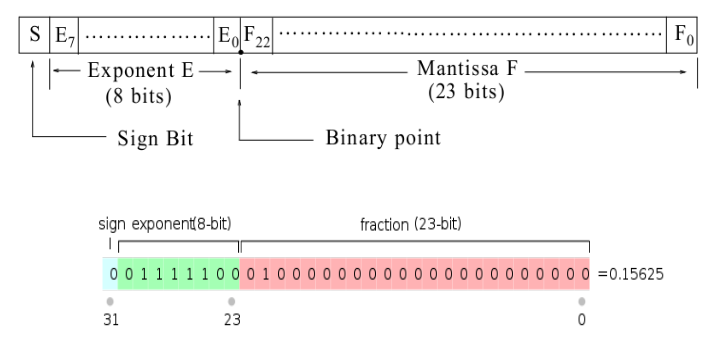
\includegraphics[scale=0.5]{./images/ieee754.png}
  \end{center}

  \bigskip
  \begin{center}
    \begin{tikzpicture}
      \node[single arrow, fill=blue!60, minimum height=1cm, single arrow head extend=2mm] (arr) {};
      \node[draw, fill=blue!10, right=0.2cm of arr] {Exo~: calculer le nombre max et min représentable};
    \end{tikzpicture}
  \end{center}
\end{frame}

% ===================================================================
\begin{frame}{IEEE 754 (SP)}
  \bigskip
  \begin{itemize}
    \item L'exposant est biaisé (en excédent) à 127. C'est-à-dire que pour
      coder un exposant $e$, on code le nombre $e+127$.
    \item Les exposants représentables vont de $-126$ à $127$ (les valeurs
      $00000000$ et $11111111$ sont réservées pour des cas exceptionnels)
    \item Les nombres sont normalisés, c'est-à-dire que la mantisse est
      entre 1 et 2.
  \end{itemize}
\end{frame}

% ===================================================================
\begin{frame}{IEEE 754 : cas exceptionnels}
  \bigskip
  \begin{itemize}
    \item Si $e = 11111111_2$ et $m=0$, le nombre représenté est $+$ ou $-$
      l'infini. Les opérations sur l'infini sont gérées correctement.
    \item Si $e = 11111111_2$ et $m \neq 0$, la représentation est
      considérée comme n'étant pas un nombre (NaN~: Not a Number).
    \item Si $e=0$ et $m=0$ on représente le nombre $+0$ ou $-0$ selon le
      signe.
    \item Si $e=0$ et $m \neq 0$ on dit que le nombre est dénormalisé.
      C'est-à-dire que la mantisse est écrite sans le 1 implicite.
  \end{itemize}
\end{frame}

% ===============================================================
\begin{frame}{Exemple de conversion  vers \texttt{ieee 754}}

  \textbf{Nombre à encoder :} $-12{,}375$

  \vspace{0.3cm}
  \textbf{1. Signe} \; : le nombre est négatif $\Rightarrow s = 1$

  \vspace{0.3cm}
  \textbf{2. Partie entière} \; : $12 = 1100_2$

  \vspace{0.3cm}
  \textbf{3. Partie fractionnaire} \; : $0{,}375$
  \[
    0{,}375 \times 2 = 0{,}75 \rightarrow 0 \qquad
    0{,}75 \times 2 = 1{,}5 \rightarrow 1 \qquad
    0{,}5 \times 2 = 1{,}0 \rightarrow 1
  \]
  \[
    \Rightarrow\; 12{,}375 = 1100{,}011_2
  \]

  \vspace{0.3cm}
  \textbf{4. Normalisation} \; : $\;1100{,}011_2 = 1{,}100011_2 \times 2^{3}$
  \begin{itemize}
    \item Mantisse : $m = 100011$
    \item Exposant réel : $e = 3$
    \item Exposant biaisé : $E = 3 + 127 = 130 = 10000010_2$
  \end{itemize}
\end{frame}

% ===============================================================
\begin{frame}{Étape 3 : assemblage des 32 bits}

  \begin{center}
  \begin{tikzpicture}[scale=0.85]
    \draw[fill=blue!20] (0,0) rectangle (1,0.8);
    \node at (0.5,0.4) {1};

    \draw[fill=green!20] (1,0) rectangle (5,0.8);
    \node at (3,0.4) {1000\,0010};

    \draw[fill=orange!20] (5,0) rectangle (11,0.8);
    \node at (8,0.4) {1000\,1100\,0000\,0000\,0000\,000};

    \node at (0.5,-0.35) {\small $s$};
    \node at (3,-0.35)   {\small exposant};
    \node at (8,-0.35)   {\small mantisse};
  \end{tikzpicture}
  \end{center}

  \vspace{0.4cm}
  \begin{block}{Résultat final}
    \[
      -12{,}375 \;\longrightarrow\;
      \underbrace{1}_{\text{signe}}\;
      \underbrace{10000010}_{\text{exposant}}\;
      \underbrace{10001100000000000000000}_{\text{mantisse}}
    \]
    \[
      \boxed{\texttt{0xC1460000}} \quad \text{(hexadécimal)}
    \]
  \end{block}

  \vspace{0.3cm}
  \textbf{Vérification :} $(-1)^1 \times 1{,}100011_2 \times 2^{130-127} = -12{,}375$ \checkmark
\end{frame}

\begin{frame}{\texttt{IEEE 754} : l'addition n'est pas commutative !}
  \begin{alertblock}{Avertissement}
    En arithmétique flottante IEEE 754, à cause des \textbf{arrondis},
    l'addition \textbf{n'est pas associative}, et dans certains cas elle
    peut même sembler \textbf{non commutative} lorsqu'on enchaîne
    plusieurs opérations ou qu'on change l'ordre des termes.
  \end{alertblock}

  \vspace{0.4cm}
  \textbf{Cause principale :} quand on additionne deux nombres d'ordres
  de grandeur très différents, le plus petit peut être \emph{entièrement
  absorbé} par l'arrondi du plus grand (\emph{absorption} / \emph{swamping}).

  \vspace{0.4cm}
  \begin{block}{Exemple classique en double précision}
    \[
      a = 1{,}0 \qquad b = 2^{-53} \qquad c = 2^{-53}
    \]
    \[
      (a + b) + c \;\neq\; a + (b + c)
    \]
  \end{block}

  \vspace{0.3cm}
  \centering
  \textit{L'ordre des opérations change le résultat !}
\end{frame}
\begin{frame}{Comment s'additionne-t-on deux flottants ?}
  \textbf{Algorithme matériel} (simplifié) pour $x + y$ :

  \vspace{0.4cm}
  \begin{enumerate}
    \item \textbf{Aligner les exposants} : on réécrit le plus petit
      exposant pour qu'il coïncide avec le plus grand. Les bits de sa
      mantisse sont \textbf{décalés vers la droite} — et les bits qui
      « sortent » sont \textbf{perdus}.
    \item \textbf{Additionner les mantisses} (avec le bit implicite).
    \item \textbf{Renormaliser} le résultat si nécessaire.
    \item \textbf{Arrondir} au format (au pair, par défaut).
  \end{enumerate}

  \vspace{0.4cm}
  \begin{block}{Le point critique}
    C'est à l'étape \textbf{1} que se joue tout le drame :
    si les exposants diffèrent de plus de $p$ bits (où $p$ est la
    précision), le plus petit nombre est \textbf{totalement
    sacrifié} au profit du plus grand.
  \end{block}

  % \vspace{0.2cm}
  % \centering
  % \begin{tikzpicture}[scale=0.9, every node/.style={font=\small}]
  %   \node[draw, rounded corners, fill=blue!10, inner sep=6pt] (x)
  %     {$x = 1{,}000\ldots0 \times 2^{0}$};
  %   \node[draw, rounded corners, fill=orange!10, inner sep=6pt,
  %         right=2cm of x] (y)
  %     {$y = 1{,}000\ldots0 \times 2^{-53}$};
  %   \draw[->, thick] (y.south) to[bend right=25]
  %     node[below, font=\scriptsize]{décalage de 53 bits vers la droite}
  %     (x.south);
  % \end{tikzpicture}
\end{frame}

% ===============================================================
\begin{frame}{\texttt{IEEE 754} : Illustration numérique}

  \textbf{Hypothèses :} double précision, $\varepsilon_{\text{mach}} = 2^{-52}$.
  Le plus petit incrément représentable autour de $1{,}0$ est
  $\text{ulp}(1) = 2^{-52}$.

  \vspace{0.4cm}
  \begin{columns}[T]
    \begin{column}{0.48\textwidth}
      \begin{block}{Calcul de $(a+b)+c$}
        \[
          a + b = 1{,}0 + 2^{-53}
        \]
        Or $2^{-53} = \tfrac{1}{2}\,\text{ulp}(1)$, donc l'arrondi
        (au pair) donne :
        \[
          a + b = 1{,}0
        \]
        Puis :
        \[
          (a+b) + c = 1{,}0
        \]
      \end{block}
    \end{column}

    \begin{column}{0.48\textwidth}
      \begin{block}{Calcul de $a+(b+c)$}
        \[
          b + c = 2^{-53} + 2^{-53} = 2^{-52}
        \]
        Cet incrément vaut exactement $\text{ulp}(1)$, donc il est
        représentable :
        \[
          a + (b+c) = 1{,}0 + 2^{-52}
        \]
      \end{block}
    \end{column}
  \end{columns}

  \vspace{0.2cm}
  \begin{center}
    \begin{tikzpicture}
      \node[draw, rounded corners, fill=red!15, inner sep=8pt] {
        $(a+b)+c = 1{,}0 \qquad \neq \qquad a+(b+c) = 1{,}0 + 2^{-52}$
      };
    \end{tikzpicture}
  \end{center}

  \vspace{0.3cm}
  \begin{alertblock}{À retenir}
    Ne jamais tester l'égalité de deux calculs flottants pour une prise de décision.
  \end{alertblock}
\end{frame}


\begin{frame}{Douglas Hofstadter et les « faux » nombres réels}

  \begin{columns}[c]
    \begin{column}{0.28\textwidth}
      \centering
      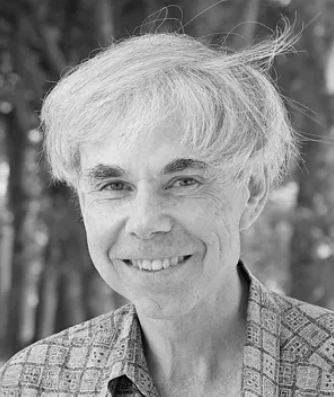
\includegraphics[scale=0.3]{./images/hofstadter.png}

      \vspace{0.2cm}
      {\scriptsize
        Douglas Hofstadter (1945--)\\
        \textit{Gödel, Escher, Bach}\\
        Prix Pulitzer 1980
      }
    \end{column}

    \begin{column}{0.70\textwidth}
      \begin{block}{}
        \itshape
        « En informatique, il n'y a pas de nombres réels. Il n'y a que
        des nombres flottants, et ils sont à peu près aussi réels que
        les personnages de dessins animés. »
      \end{block}

      \vspace{0.3cm}
      \small
      IEEE 754 ne code qu'un \textbf{ensemble fini} de valeurs, et
      chaque opération introduit un \textbf{arrondi}. Pourtant, cette
      arithmétique approximative pilote avions, réacteurs et ponts :
      la fiabilité vient des \textbf{algorithmes}, pas des nombres.
    \end{column}
  \end{columns}
\end{frame}

%============================================================================
\begin{frame}{Représentation des données symboliques}
  Certaines données ne sont pas numériques
  \begin{itemize}
    \item Enumérations, collections : couleurs,alphabets,...
    \item Ou compositions de données numériques
  \end{itemize}
Un encodage de ces données est nécessaire.
  \begin{center}
    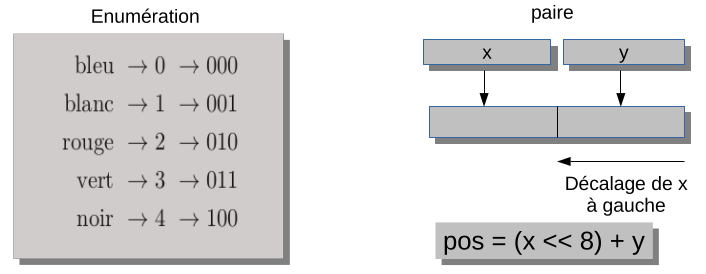
\includegraphics[scale=0.5]{./images/symb_0.png}
  \end{center}
\end{frame}

\begin{frame}{Représentation des données : codes \texttt{ASCII}}
  \begin{center}
    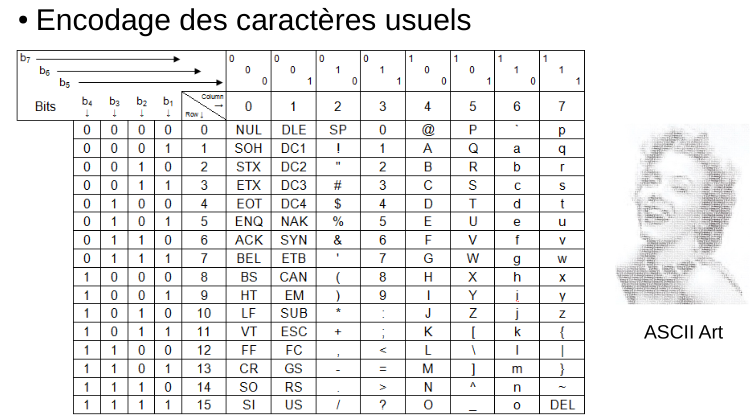
\includegraphics[scale=0.5]{./images/symb_1.png}
  \end{center}
\end{frame}

\begin{frame}{Représentation des données : codes \texttt{UTF8}}
  \begin{center}
    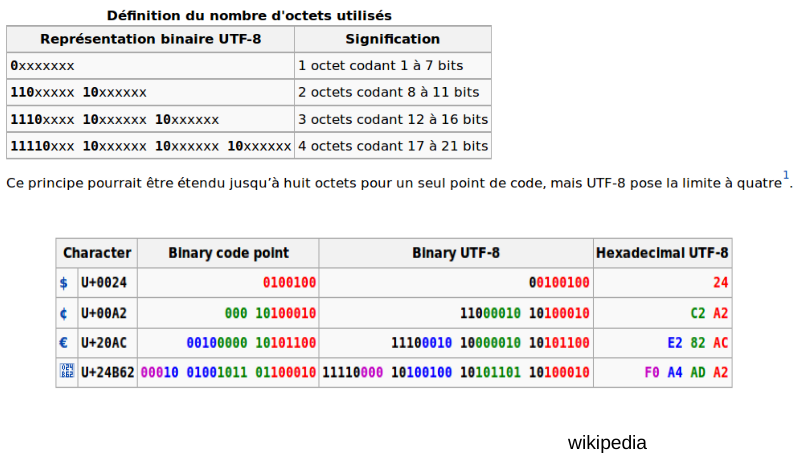
\includegraphics[scale=0.5]{./images/symb_2.png}
  \end{center}
\end{frame}

\begin{frame}{Manipulations binaires \textit{bitwise} : exemple}
  \begin{center}
    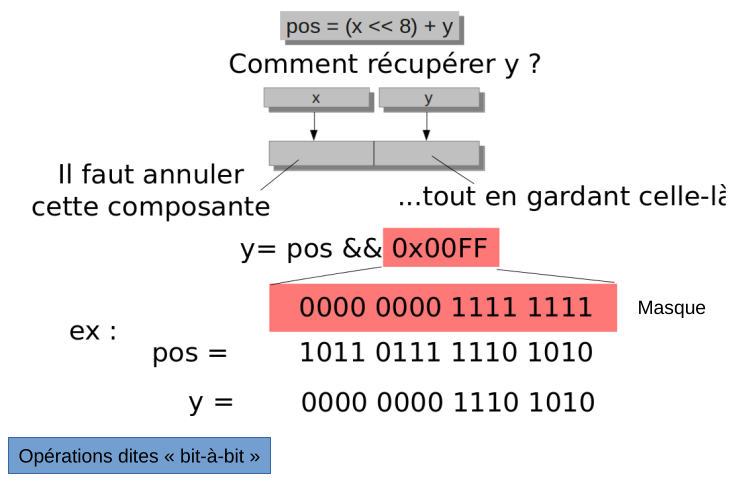
\includegraphics[scale=0.5]{./images/symb_4.png}
  \end{center}
\end{frame}

\begin{frame}{Manipulations binaires \textit{bitwise} traditionnelles}
  \begin{center}
    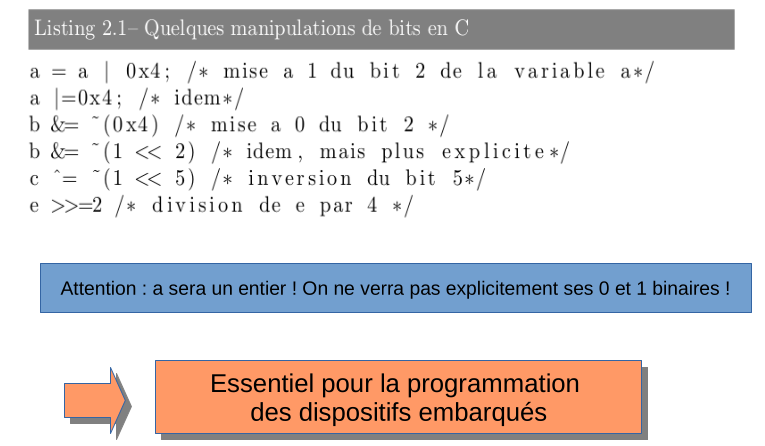
\includegraphics[scale=0.4]{./images/symb_6.png}
  \end{center}
\end{frame}

\begin{frame}{Codes détecteurs d'erreurs}
  \begin{center}
    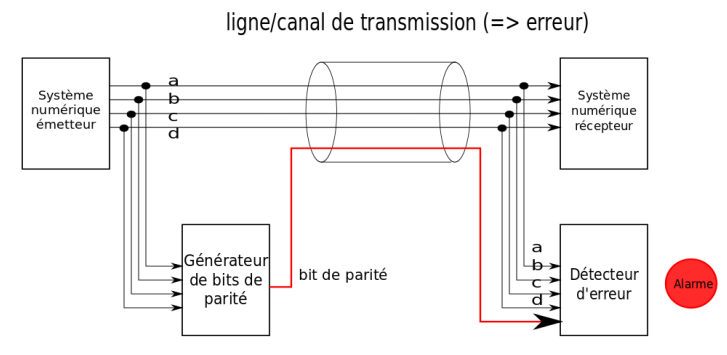
\includegraphics[scale=0.5]{./images/symb_7.png}
  \end{center}
\end{frame}

\begin{frame}{Codes détecteurs d'erreurs}
  \begin{center}
    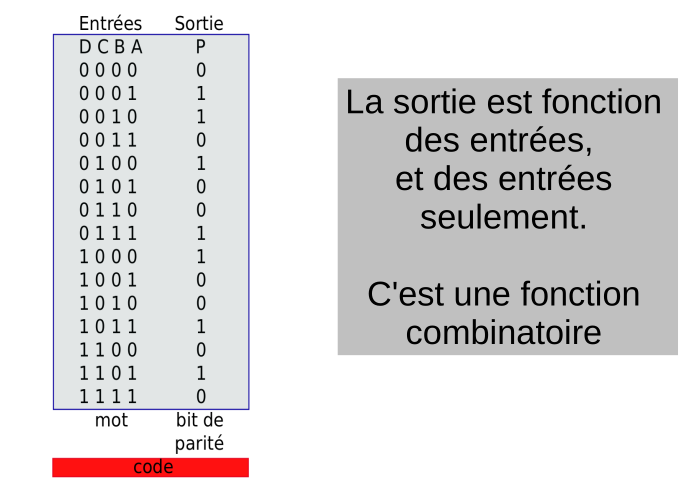
\includegraphics[scale=0.4]{./images/symb_8.png}
  \end{center}
\end{frame}

\begin{frame}{Claude Berrou et les turbocodes : correcteurs d'erreurs}

  \begin{columns}[c]
    \begin{column}{0.68\textwidth}
      \begin{block}{Une révolution née à Brest }
        \itshape
        En 1993, Claude Berrou et Alain Glavieux (ENST/IMT Atlantique) bouleversent la théorie
        de l'information en s'approchant de la \textbf{limite de Shannon},
        que les experts jugeaient inatteignable depuis 1948.
      \end{block}

      \vspace{0.3cm}
      \small
      Les \textbf{turbocodes} reposent sur un principe itératif :
      deux décodeurs élémentaires s'échangent des « croyances »
      jusqu'à converger vers le message original.

      \vspace{0.3cm}
      \textbf{Aujourd'hui :} 3G/4G, WiMAX, sondes spatiales
      (Mars Reconnaissance Orbiter, Messenger), plus de
      \textbf{4 milliards} de turbodécodeurs en circulation.
    \end{column}

    \begin{column}{0.28\textwidth}
      \centering
      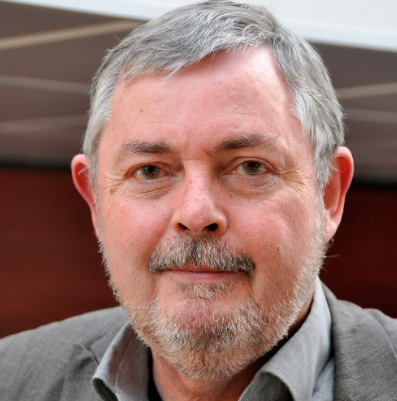
\includegraphics[scale=0.25]{./images/berrou.png}
      \vspace{0.2cm}
      {\scriptsize
        Claude Berrou (1951--)\\
        Télécom Bretagne\\
        Prix Marconi 2005\\
        Médaille Hamming 2003
      }
    \end{column}
  \end{columns}

\end{frame}

%========================================
%\section{Représentations numériques}
%========================================================================================
%\begin{frame}{Base de numération}
  \begin{itemize}
    \item On parle de \textit{base} ou \textit{radix} $r$.
    \begin{itemize}
      \item Utilisation des \textit{symboles} de $0$ à $r-1$.
      \item Notation \textit{positionnelle}
      \item Les entiers se décomposent à l'aide des coefficients des puissances de $r$.
    \end{itemize}

    \item Base 10 :
    \begin{itemize}
      \item $142 = 1\times 10^2 + 4 \times 10^1 + 2  \times 10^0$
    \end{itemize}

    \item Base 10, nombres décimaux :
    \begin{itemize}
      \item $142.34 = 1\times 10^2 + 4 \times 10^1 + 2  \times 10^0 + 3 \times 10^{-1} + 4 \times 10^{-2}$
      \item Nombre décimal $\frac{a}{10^n}$ $\rightarrow$ nombre fini de symboles.
      \item Attention : tous les nombres à virgule ne sont pas décimaux !
      \item Attention : lorsqu'on change de base, le nombre de coefficients nécessaires, pour une précision donnée, varie.
      \begin{itemize}
        \item Exemple : $0.2$ ne se représente pas avec un nombre fini de \texttt{bits} dans la base $2$ !
      \end{itemize}

    \end{itemize}
  \end{itemize}
\end{frame}

\begin{frame}{Notations non positionnelles : trois exemples}

\textbf{Chiffres romains} \hfill \textit{(additif, symboles à valeur fixe)}

\smallskip
I = 1, V = 5, X = 10, L = 50, C = 100, D = 500, M = 1000

\smallskip
Exemple : MCMXCIV = 1000 + (1000-100) + (100-10) + (5-1) = \textbf{1994}

\vspace{0.6cm}

\textbf{Système unaire} \hfill \textit{(additif pur, une marque par unité)}

\smallskip
\texttt{|||||} = 5 \qquad \texttt{|||||||} = 7 \quad \textit{(ou groupes de 5)}

\vspace{0.6cm}

\textbf{Hiéroglyphes égyptiens} \hfill \textit{(additif, un symbole par puissance de 10)}

\smallskip
\begin{tabular}{ll}
$\vert$ = 1 & $\cap$ = 10 \\
$\curlywedge$ = 100 & $\odot$ = 1000 \\
\end{tabular}

\smallskip
24 s'écrit : deux « anses » + quatre « traits » --- \textbf{l'ordre n'importe pas}

\vspace{0.4cm}

\centering
\footnotesize\itshape
Dans tous ces systèmes, la position d'un symbole ne modifie jamais sa valeur.

\end{frame}

\begin{frame}{Généralisation}
  La formule générale pour la base 10 est bien entendu :
  $$ x = \sum_{i=-\infty}^{i=+\infty} c_i.10^i, c_i \in \{0,\dots,9 \}$$
  et se généralise :
  $$ \forall r, x = \sum_{i=-\infty}^{i=+\infty} c_{i,r}.r^i, c_{i,r} \in \{0,\dots,(r-1)\}$$
  Lors des changements de base, il faut une notation pour préciser la base de représentation.
  \begin{itemize}
    \item Par exemple : $ 142_{10} = 10001110_{2}$
    \item En logiciel : $ 142_{10} = \text{\texttt{0b10001110}} = \text{\texttt{0x8e}} = \text{\texttt{0o216}}$

    \end{itemize}
\end{frame}

\begin{frame}{Compter en binaire : convertir par table}

  \begin{columns}
    \begin{column}{0.5\textwidth}
      \begin{table}[h]
        \centering
        \resizebox{!}{0.44\textheight}{%
        \begin{tabular}{c|ccccc}
          \toprule
          \multirow{2}{*}{\textbf{Decimal count}} & \multicolumn{5}{c}{\textbf{Binary count}} \\
          \cmidrule(l){2-6} & \textbf{16s} & \textbf{8s} & \textbf{4s} & \textbf{2s} & \textbf{1s} \\
          \midrule
          0  &   &   &   &   & 0 \\
          1  &   &   &   &   & 1 \\
          2  &   &   &   & 1 & 0 \\
          3  &   &   &   & 1 & 1 \\
          4  &   &   & 1 & 0 & 0 \\
          5  &   &   & 1 & 0 & 1 \\
          6  &   &   & 1 & 1 & 0 \\
          7  &   &   & 1 & 1 & 1 \\
          8  &   & 1 & 0 & 0 & 0 \\
          9  &   & 1 & 0 & 0 & 1 \\
          10 &   & 1 & 0 & 1 & 0 \\
          11 &   & 1 & 0 & 1 & 1 \\
          12 &   & 1 & 1 & 0 & 0 \\
          13 &   & 1 & 1 & 0 & 1 \\
          14 &   & 1 & 1 & 1 & 0 \\
          15 &   & 1 & 1 & 1 & 1 \\
          16 & 1 & 0 & 0 & 0 & 0 \\
          17 & 1 & 0 & 0 & 0 & 1 \\
          18 & 1 & 0 & 0 & 1 & 0 \\
          19 & 1 & 0 & 0 & 1 & 1 \\
          \midrule
          & $2^4$ & $2^3$ & $2^2$ & $2^1$ & $2^0$ \\
          \cmidrule(l){2-6}
          & \multicolumn{5}{c}{Powers of 2} \\
          \bottomrule
        \end{tabular}
        % \vspace{1pt}
        % \hspace{2.cm}\textbf{MSB} \hfill \textbf{LSB}\hspace{0.1cm}
        } %resizex
      \end{table}
    \end{column}

    \begin{column}{0.5\textwidth}
      \begin{table}[h]
      \centering
        \resizebox{!}{0.44\textheight}{
        \begin{tabular}{cccc}
        \toprule
        \textbf{Décimal} & \textbf{Binaire} & \textbf{Octal} & \textbf{Hexadécimal} \\
        \midrule
        0  & 0000 & 0  & 0 \\
        1  & 0001 & 1  & 1 \\
        2  & 0010 & 2  & 2 \\
        3  & 0011 & 3  & 3 \\
        4  & 0100 & 4  & 4 \\
        5  & 0101 & 5  & 5 \\
        6  & 0110 & 6  & 6 \\
        7  & 0111 & 7  & 7 \\
        8  & 1000 & 10 & 8 \\
        9  & 1001 & 11 & 9 \\
        10 & 1010 & 12 & A \\
        11 & 1011 & 13 & B \\
        12 & 1100 & 14 & C \\
        13 & 1101 & 15 & D \\
        14 & 1110 & 16 & E \\
        15 & 1111 & 17 & F \\
        \bottomrule
      \end{tabular}
      }
      \end{table}
    \end{column}

  \end{columns}
\end{frame}

\begin{frame}{A quoi ça sert ?}
  \begin{center}
    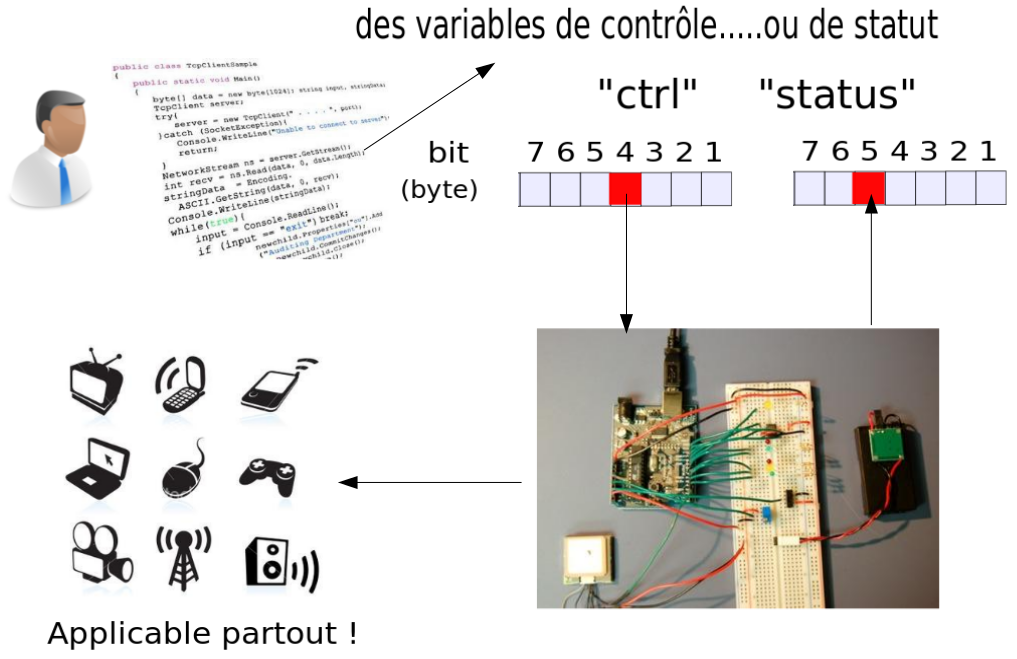
\includegraphics[scale=0.3]{./images/numbers_2.png}
  \end{center}
\end{frame}

\begin{frame}{A quoi ça sert ?}
  \begin{columns}
    \begin{column}{0.5\textwidth}
      \begin{center}
        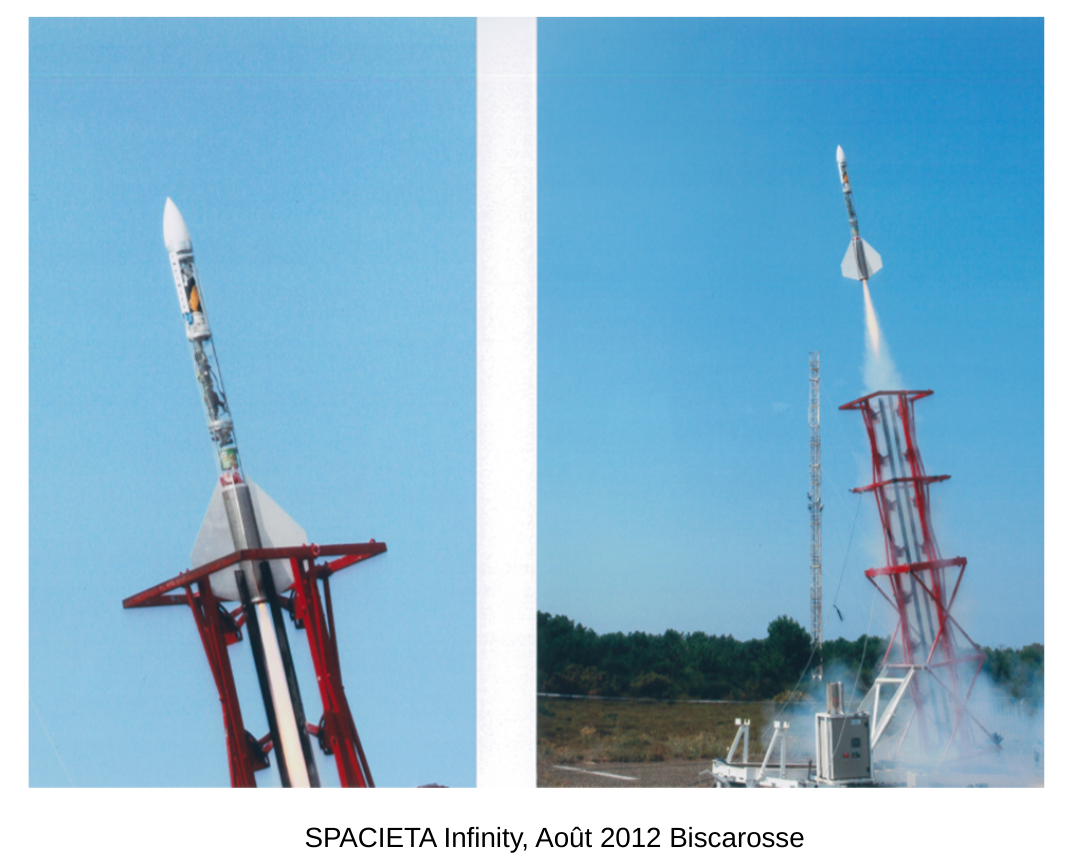
\includegraphics[scale=0.18]{./images/spacieta.png}
      \end{center}
    \end{column}

    \begin{column}{0.5\textwidth}
      \begin{center}
        \includegraphics[scale=0.18]{/home/jcll/Dropbox/IMAGES_TECHNIQUES/JOG.jpg}
      \end{center}
      JOG : conçu  à l'ENSTA Bretagne pour l'enseignement 1A.
    \end{column}
  \end{columns}
\end{frame}

\begin{frame}{Conversions entre bases : par table}
  \begin{center}
    \small $101101_{2} = \text{10\_1101}_{2} = \text{0010\_1101}_{2} = 2D_{16} = \mathbf{0x2D}$
  \end{center}

  \smallskip
  {\small Dans le cas de nombres fractionnaires, on rajoute des 0 à droite de la
  partie fractionnaire. Ainsi~:}

  \begin{center}
    \small le nombre $1011.01_{2} = \text{1011.0100}_{2} = B.4_{16}$
  \end{center}

  \smallskip
  {\small On procède de même pour la traduction octale.}

  \begin{center}
    \small $(10110001101011.1111)_{2} = (\text{101 110 001 101 011}.\text{111 100})_{2} = (36153.74)_{8}$
  \end{center}

  \smallskip
  \begin{center}
    \small
    \begin{tabular}{cccc}
      4 & 7 & . & F \quad E \\[-2pt]
      $\downarrow$ & $\downarrow$ & & $\downarrow$ \qquad $\downarrow$ \\[-2pt]
      0100 & 0111 & . & 1111 \quad 1110
    \end{tabular}

    \smallskip
    \small $47.\text{FE}_{16} \approx 1000111.1111111_{2}$
  \end{center}

\end{frame}

\begin{frame}{Conversions entre bases : par calcul}
  \begin{center}
    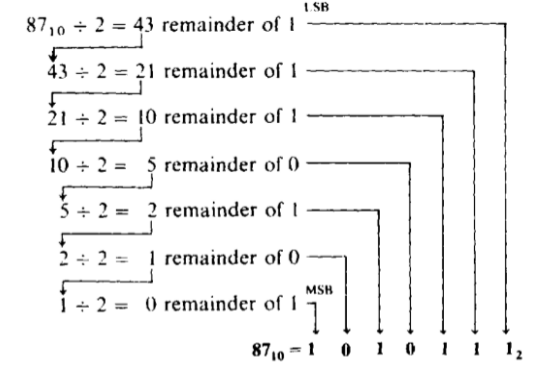
\includegraphics[scale=0.5]{./images/numbers_5.png}
  \end{center}
\end{frame}

\begin{frame}{Conversions entre bases : par calcul}
  \begin{center}
    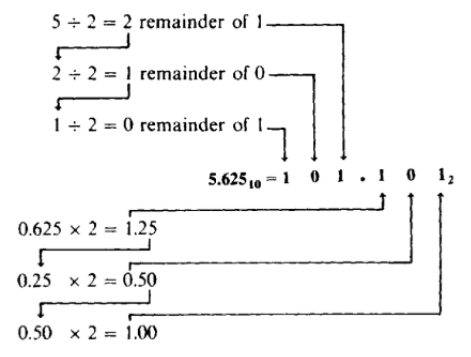
\includegraphics[scale=0.5]{./images/numbers_6.png}
  \end{center}
\end{frame}

\begin{frame}{Conversions entre bases : par calcul}
  \begin{center}
    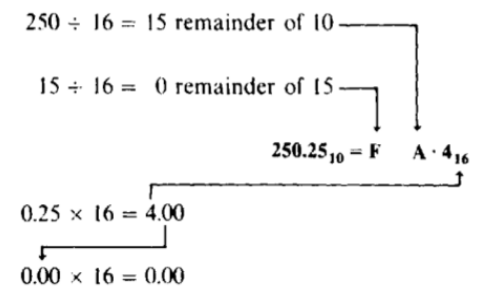
\includegraphics[scale=0.5]{./images/numbers_7.png}
  \end{center}
\end{frame}

\begin{frame}{Autres codes binaires : BCD décimal codé binaire}
  \begin{center}
    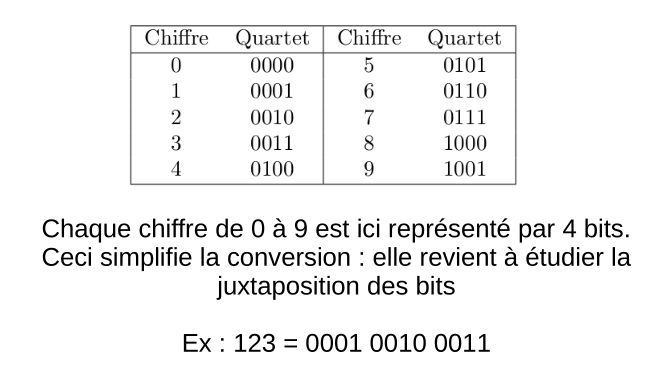
\includegraphics[scale=0.5]{./images/numbers_8.png}
  \end{center}
\end{frame}

\begin{frame}{Autres codes binaires : code de gray ou binaire réfléchi}
  \begin{center}
    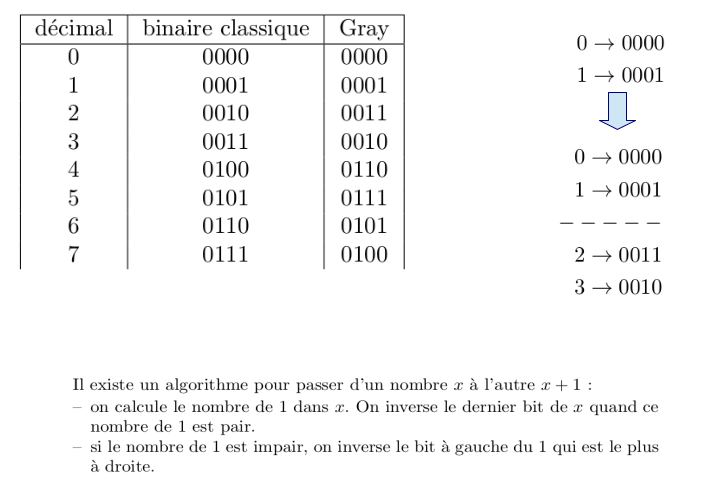
\includegraphics[scale=0.4]{./images/numbers_9.png}
  \end{center}
\end{frame}

\begin{frame}{Entiers positifs ou \texttt{unsigned}}
  \bigskip
  Soit un nombre $W$ de bits et soit $\vec{x} = [x_{w-1},x_{w-2},\ldots,x_0]$ de
  bits. Nous avons vu précédemment (sans la nommer) que la simple fonction~:
  \[
    B2U_w(\vec{x}) \doteq \sum_{i=0}^{w-1} x_i 2^i
  \]
  définit la valeur non-signée ("unsigned") de $\vec{x}$, dans $\mathbb{N}$.
  Les valeurs limites de cette fonction sont~:
  \[
    \begin{cases}
      UMax_w = \sum_{i=0}^{w-1} 2^i = 2^w - 1 \\
      UMmin_w = \sum_{i=0}^{w-1} 0 = 0
    \end{cases}
  \]
  On a donc~:
  \[
    B2U_w : \{0,1\}^w \to \{0,\ldots,2^w-1\}
  \]
\end{frame}

\begin{frame}{Complément à 2 sur w bits}
 \medskip
  \small
  De manière similaire, on définit désormais la fonction qui permet de
  calculer la valeur du vecteur $\vec{x}$ dans le cas d'une valeur signée,
  c'est-à-dire négative ou positive, \textbf{en complément à 2}.
  \[
    B2T_w(\vec{x}) \doteq -x_{w-1}2^{w-1} + \sum_{i=0}^{w-2} x_i 2^i
  \]
  Désormais, le bit de poids fort, le plus à gauche, contribue de manière
  négative à la somme totale. Précisons également que le 'T' vient de
  "two's complement". Calculons les valeurs min et max de cette fonction.
  Pour $\vec{x} = [10\ldots0]$ et $\vec{x} = [01\ldots1]$ respectivement, on
  trouve~:
  \[
    \begin{cases}
      TMin_w = -2^{w-1} \\
      TMax_w = \displaystyle\sum_{i=0}^{w-2} 2^i = 2^{w-1} - 1
    \end{cases}
  \]
  On a donc~:
  \[
    B2U_w : \{0,1\}^w \to \{-2^{w-1},\ldots,2^{w-1}-1\}
  \]
  On pourra également dénoter cette fonction $C_{2,w}(\vec{x})$.
\end{frame}

% ===================================================================
\begin{frame}{Complément à 2 sur w bits}

  \bigskip
  \begin{center}
    \renewcommand{\arraystretch}{1.15}
    \begin{tabular}{|c|c||c|}
      \hline
      \textbf{signé} & \textbf{bit vector} & \textbf{non-signé} \\
      \hline
      $-4$ & 100 & 4 \\ \hline
      $-3$ & 101 & 5 \\ \hline
      $-2$ & 110 & 6 \\ \hline
      $-1$ & 111 & 7 \\ \hline
      $0$  & 000 & 0 \\ \hline
      $1$  & 001 & 1 \\ \hline
      $2$  & 010 & 2 \\ \hline
      $3$  & 011 & 3 \\ \hline
    \end{tabular}
  \end{center}
\end{frame}

% ===================================================================
\begin{frame}{Nombres négatifs}

  \bigskip
  Le complément à 1 d'un nombre binaire consiste à simplement inverser tous
  ses bits.
  \medskip
  Le complément à 2 d'un nombre binaire s'obtient ainsi:
  \begin{itemize}
    \item On parcourt le nombre en partant de la droite (bit de poids faible).
    \item On recopie tel quel tous les bits tant qu'on n'a pas rencontré le premier 1.
    \item On recopie ce premier 1.
    \item On inverse tous les bits suivants (à gauche de ce 1).
  \end{itemize}
  Il existe toutefois une autre méthode, qui se retient plus facilement
  (peut-être). Elle consiste en une formule simple~:

  \bigskip
  \begin{columns}
    \begin{column}{0.35\textwidth}
      \colorbox{blue!20}{\parbox{0.9\textwidth}{\small\textbf{Attention~!!!!}\\
      $-134$ nécessite 9 bits et non 8}}
    \end{column}
    \begin{column}{0.65\textwidth}
      \begin{tikzpicture}
        \node[draw, fill=gray!30, minimum width=3cm, minimum height=1cm, font=\Large] (box) {$-X = \overline{X} + 1$};
        \node[below=0.9cm of box, align=left, xshift=0.3cm] (lab) {\footnotesize Addition classique\\\footnotesize (et non « OU » binaire)};
        \draw[-{Latex[length=3mm]}] (lab.north -| box.south) -- (box.south);
      \end{tikzpicture}
    \end{column}
  \end{columns}
\end{frame}

% ===================================================================
\begin{frame}{Nombres négatifs : représentations obsolètes}
  \bigskip
  \small
  La représentation en magnitude signée est simplement~:
  \[
    B2S_w(\vec{x}) \doteq (-1)^{x_{w-1}} \sum_{i=0}^{w-2} x_i 2^i
  \]
  Il existe également une représentation des nombres en complément à 1,
  très légèrement différente du complément à 2.
  \[
    B2T_w(\vec{x}) \doteq -x_{w-1}(2^{w-1}-1) + \sum_{i=0}^{w-2} x_i 2^i
  \]

  \bigskip
  \begin{center}
    \begin{tikzpicture}
      %\node[arrow, fill=red, minimum height=1cm, arrow head extend=2mm] (arr) {};
      \node[draw, fill=blue!10, align=center] {Ces représentations proposent 2 encodages pour 0~!};
    \end{tikzpicture}
  \end{center}

  \normalsize
  Dans le cas de la magnitude signée~:\\
  $+0 = 0\ldots.0$ et $-0 = 10\ldots0$
\end{frame}

% ===================================================================
\begin{frame}{Nombres négatifs : résumé}
  \begin{columns}[t]
    \begin{column}{0.42\textwidth}
      \tiny
      \renewcommand{\arraystretch}{1.05}
      \begin{tabular}{|c|c|}
        \hline
        \textbf{Signed decimal} & \textbf{8-bit 2's compl.} \\
        \hline
        $+127$ & 0111 1111 \\
        $+126$ & 0111 1110 \\
        $+125$ & 0111 1101 \\
        $\vdots$ & $\vdots$ \\
        $+1$ & 0000 0001 \\
        $+0$ & 0000 0000 \\
        \hline
        $-1$ & 1111 1111 \\
        $-2$ & 1111 1110 \\
        $\vdots$ & $\vdots$ \\
        $-125$ & 1000 0011 \\
        $-126$ & 1000 0010 \\
        $-127$ & 1000 0001 \\
        $-128$ & 1000 0000 \\
        \hline
      \end{tabular}
    \end{column}
    \begin{column}{0.58\textwidth}
      \small
      \begin{center}
        \begin{tikzpicture}
          \node[draw, fill=gray!30, minimum width=2.5cm, minimum height=0.9cm, font=\large] {$-X = \overline{X} + 1$};
        \end{tikzpicture}
      \end{center}

      \bigskip
      \colorbox{orange!40}{
      \begin{minipage}{0.95\textwidth}
        $-125\; ? =$

        \medskip
        $125 \quad = \quad 111\,1101$

        \medskip
        $/125 \quad = \quad \textcolor{red}{1}\,000\,0010$

        \medskip
        $/125+1 = 1\,000\,0011$
      \end{minipage}}
    \end{column}
  \end{columns}

  \bigskip
  \small
  Noter que les nombres en complément à 2 sont négatifs s'ils présentent un
  MSB à 1~!\\
  125 se représente sur 7 bits, mais pas $-125$~: il faut 8 bits
\end{frame}

% ===================================================================
\begin{frame}{\LARGE Exemple~: $-3$ sur 3 bits}


  \begin{columns}[t]
    \begin{column}{0.62\textwidth}
      \begin{itemize}
        \item $3_{10} = 011_2$
        \item $-3_{10} = /3_{10} + 1 = 100_2 + 1 = 101_2 = 5_{10}$~????
        \begin{itemize}
          \item 5 ne peut pas être représenté sur 3 bits, si on y
            représente également les nombres négatifs.
        \end{itemize}
      \end{itemize}

      \bigskip
      \colorbox{blue!30}{\parbox{0.95\textwidth}{\centering
        Pour un nombre donné de bits,\\
        il faut s'entendre sur le fait\\
        que la représentation d'un nombre est signée ou non}}
    \end{column}
    \begin{column}{0.35\textwidth}
      \small
      \begin{tabular}{cc}
        $+3$ & 011 \\
        $+2$ & 010 \\
        $+1$ & 001 \\
        $+0$ & 000 \\
        $-1$ & 111 \\
        $-2$ & 110 \\
        $-3$ & 101 \\
        $-4$ & 100 \\
      \end{tabular}
    \end{column}
  \end{columns}
\end{frame}

% ===================================================================
\begin{frame}{Addition et soustraction}

  \bigskip
  \textbf{Addition}~: classique
  \hfill
  \begin{minipage}{0.55\textwidth}
    \centering
    \renewcommand{\arraystretch}{1.2}
    \begin{tabular}{|l|r|}
      \hline
      & \textbf{Addition} \\
      \hline
      calcul & \begin{tabular}{r}0110\\ $+$0011\end{tabular} \\
      \hline
      retenus & 11 \\
      \hline
      résultat & 1001 \\
      \hline
    \end{tabular}
  \end{minipage}

  \bigskip
  \textbf{Soustraction : x - y}

  \small
  \begin{enumerate}
    \item on additionne $x$ et le complément à 2 de $y$
    \item si le résultat présente une retenue finale, on l'oublie~!
    \item s'il n'y a pas de retenue finale, on prend le complément à 2 du
      résultat et on place un signe "-" devant le nombre.
  \end{enumerate}

  \medskip
  \textbf{exemple}~: $x = 1101100_2$ et $y = 1011011_2$
  \[
    1101100 + 0100101 = 1\,0010001
  \]
  Le résultat est donc $x - y = 0010001_2$

  \hfill\tiny 108-91
\end{frame}

% ===================================================================
\begin{frame}{\LARGE Nombre en virgule fixe : ou \textit{fixed point}}

  \bigskip
  \begin{itemize}
    \item Déjà vu précédemment\ldots
    \item Le calculateur numérique devra connaître la position de la
      virgule, fixée une bonne fois pour toute.
    \item Impact sur les opérations classiques~:
    \begin{itemize}
      \item Le résultat de l'addition hérite de la position de la virgule
        identique à celle dans les opérandes
      \item Cela est changé pour les autres opérations.
    \end{itemize}
  \end{itemize}
\end{frame}

% ===================================================================
\begin{frame}{Nombres en virgule flottante : norme \texttt{ieee754}}

  \begin{center}
    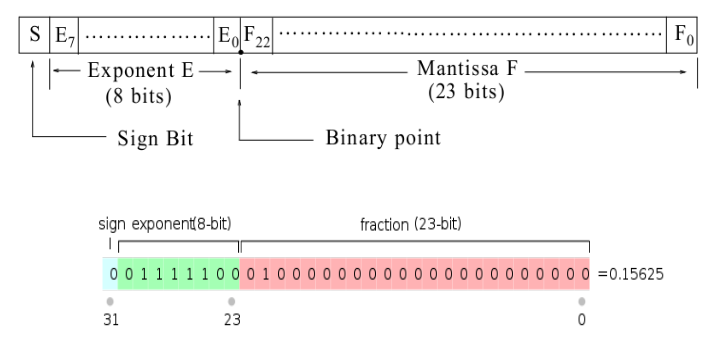
\includegraphics[scale=0.5]{./images/ieee754.png}
  \end{center}

  \bigskip
  \begin{center}
    \begin{tikzpicture}
      \node[single arrow, fill=blue!60, minimum height=1cm, single arrow head extend=2mm] (arr) {};
      \node[draw, fill=blue!10, right=0.2cm of arr] {Exo~: calculer le nombre max et min représentable};
    \end{tikzpicture}
  \end{center}
\end{frame}

% ===================================================================
\begin{frame}{IEEE 754 (SP)}
  \bigskip
  \begin{itemize}
    \item L'exposant est biaisé (en excédent) à 127. C'est-à-dire que pour
      coder un exposant $e$, on code le nombre $e+127$.
    \item Les exposants représentables vont de $-126$ à $127$ (les valeurs
      $00000000$ et $11111111$ sont réservées pour des cas exceptionnels)
    \item Les nombres sont normalisés, c'est-à-dire que la mantisse est
      entre 1 et 2.
  \end{itemize}
\end{frame}

% ===================================================================
\begin{frame}{IEEE 754 : cas exceptionnels}
  \bigskip
  \begin{itemize}
    \item Si $e = 11111111_2$ et $m=0$, le nombre représenté est $+$ ou $-$
      l'infini. Les opérations sur l'infini sont gérées correctement.
    \item Si $e = 11111111_2$ et $m \neq 0$, la représentation est
      considérée comme n'étant pas un nombre (NaN~: Not a Number).
    \item Si $e=0$ et $m=0$ on représente le nombre $+0$ ou $-0$ selon le
      signe.
    \item Si $e=0$ et $m \neq 0$ on dit que le nombre est dénormalisé.
      C'est-à-dire que la mantisse est écrite sans le 1 implicite.
  \end{itemize}
\end{frame}

% ===============================================================
\begin{frame}{Exemple de conversion  vers \texttt{ieee 754}}

  \textbf{Nombre à encoder :} $-12{,}375$

  \vspace{0.3cm}
  \textbf{1. Signe} \; : le nombre est négatif $\Rightarrow s = 1$

  \vspace{0.3cm}
  \textbf{2. Partie entière} \; : $12 = 1100_2$

  \vspace{0.3cm}
  \textbf{3. Partie fractionnaire} \; : $0{,}375$
  \[
    0{,}375 \times 2 = 0{,}75 \rightarrow 0 \qquad
    0{,}75 \times 2 = 1{,}5 \rightarrow 1 \qquad
    0{,}5 \times 2 = 1{,}0 \rightarrow 1
  \]
  \[
    \Rightarrow\; 12{,}375 = 1100{,}011_2
  \]

  \vspace{0.3cm}
  \textbf{4. Normalisation} \; : $\;1100{,}011_2 = 1{,}100011_2 \times 2^{3}$
  \begin{itemize}
    \item Mantisse : $m = 100011$
    \item Exposant réel : $e = 3$
    \item Exposant biaisé : $E = 3 + 127 = 130 = 10000010_2$
  \end{itemize}
\end{frame}

% ===============================================================
\begin{frame}{Étape 3 : assemblage des 32 bits}

  \begin{center}
  \begin{tikzpicture}[scale=0.85]
    \draw[fill=blue!20] (0,0) rectangle (1,0.8);
    \node at (0.5,0.4) {1};

    \draw[fill=green!20] (1,0) rectangle (5,0.8);
    \node at (3,0.4) {1000\,0010};

    \draw[fill=orange!20] (5,0) rectangle (11,0.8);
    \node at (8,0.4) {1000\,1100\,0000\,0000\,0000\,000};

    \node at (0.5,-0.35) {\small $s$};
    \node at (3,-0.35)   {\small exposant};
    \node at (8,-0.35)   {\small mantisse};
  \end{tikzpicture}
  \end{center}

  \vspace{0.4cm}
  \begin{block}{Résultat final}
    \[
      -12{,}375 \;\longrightarrow\;
      \underbrace{1}_{\text{signe}}\;
      \underbrace{10000010}_{\text{exposant}}\;
      \underbrace{10001100000000000000000}_{\text{mantisse}}
    \]
    \[
      \boxed{\texttt{0xC1460000}} \quad \text{(hexadécimal)}
    \]
  \end{block}

  \vspace{0.3cm}
  \textbf{Vérification :} $(-1)^1 \times 1{,}100011_2 \times 2^{130-127} = -12{,}375$ \checkmark
\end{frame}

\begin{frame}{\texttt{IEEE 754} : l'addition n'est pas commutative !}
  \begin{alertblock}{Avertissement}
    En arithmétique flottante IEEE 754, à cause des \textbf{arrondis},
    l'addition \textbf{n'est pas associative}, et dans certains cas elle
    peut même sembler \textbf{non commutative} lorsqu'on enchaîne
    plusieurs opérations ou qu'on change l'ordre des termes.
  \end{alertblock}

  \vspace{0.4cm}
  \textbf{Cause principale :} quand on additionne deux nombres d'ordres
  de grandeur très différents, le plus petit peut être \emph{entièrement
  absorbé} par l'arrondi du plus grand (\emph{absorption} / \emph{swamping}).

  \vspace{0.4cm}
  \begin{block}{Exemple classique en double précision}
    \[
      a = 1{,}0 \qquad b = 2^{-53} \qquad c = 2^{-53}
    \]
    \[
      (a + b) + c \;\neq\; a + (b + c)
    \]
  \end{block}

  \vspace{0.3cm}
  \centering
  \textit{L'ordre des opérations change le résultat !}
\end{frame}
\begin{frame}{Comment s'additionne-t-on deux flottants ?}
  \textbf{Algorithme matériel} (simplifié) pour $x + y$ :

  \vspace{0.4cm}
  \begin{enumerate}
    \item \textbf{Aligner les exposants} : on réécrit le plus petit
      exposant pour qu'il coïncide avec le plus grand. Les bits de sa
      mantisse sont \textbf{décalés vers la droite} — et les bits qui
      « sortent » sont \textbf{perdus}.
    \item \textbf{Additionner les mantisses} (avec le bit implicite).
    \item \textbf{Renormaliser} le résultat si nécessaire.
    \item \textbf{Arrondir} au format (au pair, par défaut).
  \end{enumerate}

  \vspace{0.4cm}
  \begin{block}{Le point critique}
    C'est à l'étape \textbf{1} que se joue tout le drame :
    si les exposants diffèrent de plus de $p$ bits (où $p$ est la
    précision), le plus petit nombre est \textbf{totalement
    sacrifié} au profit du plus grand.
  \end{block}

  % \vspace{0.2cm}
  % \centering
  % \begin{tikzpicture}[scale=0.9, every node/.style={font=\small}]
  %   \node[draw, rounded corners, fill=blue!10, inner sep=6pt] (x)
  %     {$x = 1{,}000\ldots0 \times 2^{0}$};
  %   \node[draw, rounded corners, fill=orange!10, inner sep=6pt,
  %         right=2cm of x] (y)
  %     {$y = 1{,}000\ldots0 \times 2^{-53}$};
  %   \draw[->, thick] (y.south) to[bend right=25]
  %     node[below, font=\scriptsize]{décalage de 53 bits vers la droite}
  %     (x.south);
  % \end{tikzpicture}
\end{frame}

% ===============================================================
\begin{frame}{\texttt{IEEE 754} : Illustration numérique}

  \textbf{Hypothèses :} double précision, $\varepsilon_{\text{mach}} = 2^{-52}$.
  Le plus petit incrément représentable autour de $1{,}0$ est
  $\text{ulp}(1) = 2^{-52}$.

  \vspace{0.4cm}
  \begin{columns}[T]
    \begin{column}{0.48\textwidth}
      \begin{block}{Calcul de $(a+b)+c$}
        \[
          a + b = 1{,}0 + 2^{-53}
        \]
        Or $2^{-53} = \tfrac{1}{2}\,\text{ulp}(1)$, donc l'arrondi
        (au pair) donne :
        \[
          a + b = 1{,}0
        \]
        Puis :
        \[
          (a+b) + c = 1{,}0
        \]
      \end{block}
    \end{column}

    \begin{column}{0.48\textwidth}
      \begin{block}{Calcul de $a+(b+c)$}
        \[
          b + c = 2^{-53} + 2^{-53} = 2^{-52}
        \]
        Cet incrément vaut exactement $\text{ulp}(1)$, donc il est
        représentable :
        \[
          a + (b+c) = 1{,}0 + 2^{-52}
        \]
      \end{block}
    \end{column}
  \end{columns}

  \vspace{0.2cm}
  \begin{center}
    \begin{tikzpicture}
      \node[draw, rounded corners, fill=red!15, inner sep=8pt] {
        $(a+b)+c = 1{,}0 \qquad \neq \qquad a+(b+c) = 1{,}0 + 2^{-52}$
      };
    \end{tikzpicture}
  \end{center}

  \vspace{0.3cm}
  \begin{alertblock}{À retenir}
    Ne jamais tester l'égalité de deux calculs flottants pour une prise de décision.
  \end{alertblock}
\end{frame}


\begin{frame}{Douglas Hofstadter et les « faux » nombres réels}

  \begin{columns}[c]
    \begin{column}{0.28\textwidth}
      \centering
      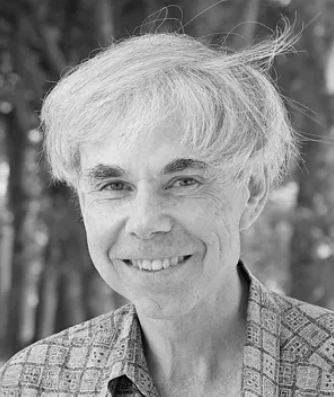
\includegraphics[scale=0.3]{./images/hofstadter.png}

      \vspace{0.2cm}
      {\scriptsize
        Douglas Hofstadter (1945--)\\
        \textit{Gödel, Escher, Bach}\\
        Prix Pulitzer 1980
      }
    \end{column}

    \begin{column}{0.70\textwidth}
      \begin{block}{}
        \itshape
        « En informatique, il n'y a pas de nombres réels. Il n'y a que
        des nombres flottants, et ils sont à peu près aussi réels que
        les personnages de dessins animés. »
      \end{block}

      \vspace{0.3cm}
      \small
      IEEE 754 ne code qu'un \textbf{ensemble fini} de valeurs, et
      chaque opération introduit un \textbf{arrondi}. Pourtant, cette
      arithmétique approximative pilote avions, réacteurs et ponts :
      la fiabilité vient des \textbf{algorithmes}, pas des nombres.
    \end{column}
  \end{columns}
\end{frame}

%============================================================================
\begin{frame}{Représentation des données symboliques}
  Certaines données ne sont pas numériques
  \begin{itemize}
    \item Enumérations, collections : couleurs,alphabets,...
    \item Ou compositions de données numériques
  \end{itemize}
Un encodage de ces données est nécessaire.
  \begin{center}
    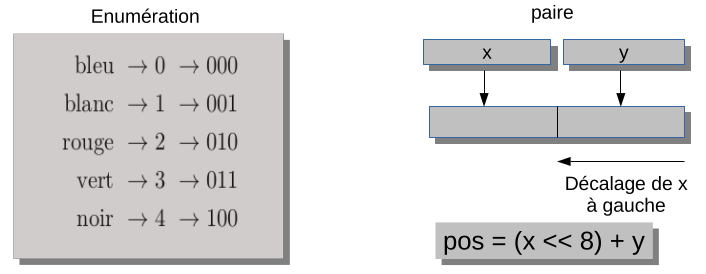
\includegraphics[scale=0.5]{./images/symb_0.png}
  \end{center}
\end{frame}

\begin{frame}{Représentation des données : codes \texttt{ASCII}}
  \begin{center}
    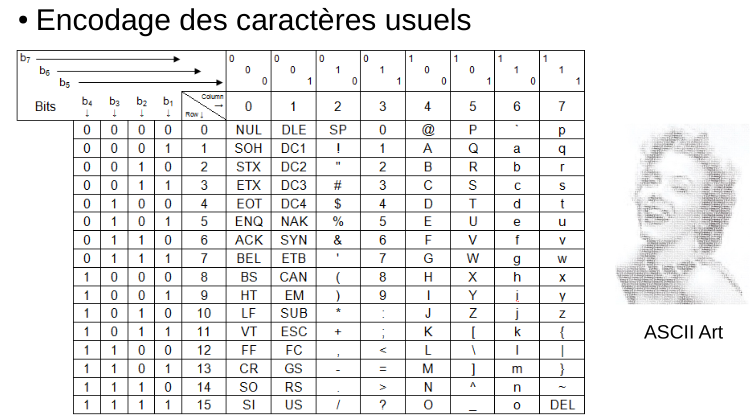
\includegraphics[scale=0.5]{./images/symb_1.png}
  \end{center}
\end{frame}

\begin{frame}{Représentation des données : codes \texttt{UTF8}}
  \begin{center}
    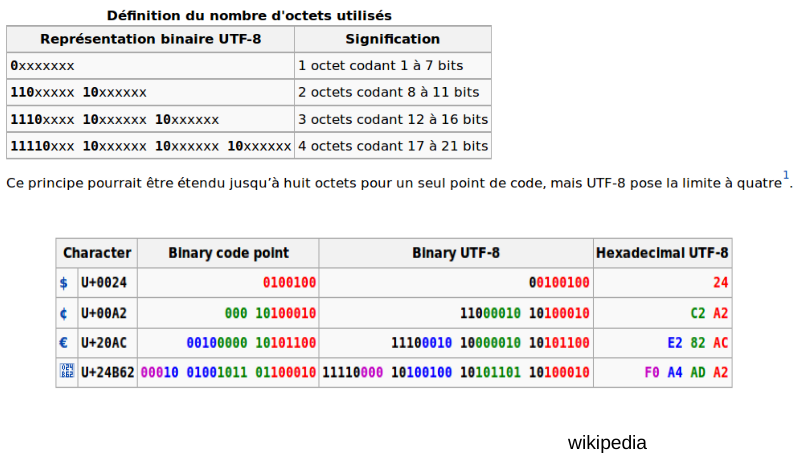
\includegraphics[scale=0.5]{./images/symb_2.png}
  \end{center}
\end{frame}

\begin{frame}{Manipulations binaires \textit{bitwise} : exemple}
  \begin{center}
    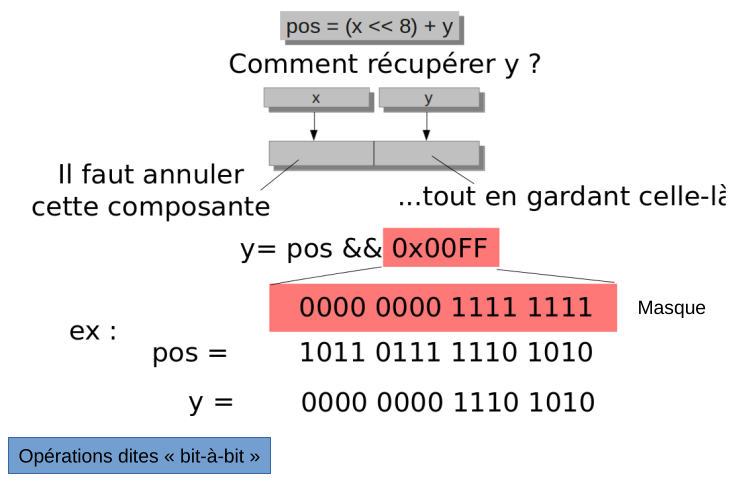
\includegraphics[scale=0.5]{./images/symb_4.png}
  \end{center}
\end{frame}

\begin{frame}{Manipulations binaires \textit{bitwise} traditionnelles}
  \begin{center}
    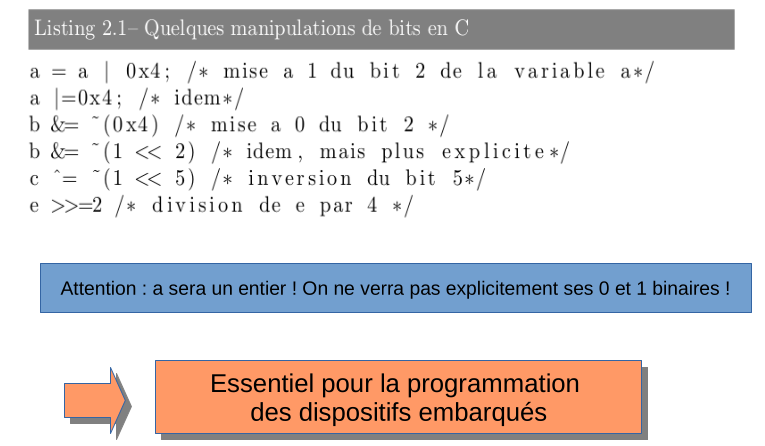
\includegraphics[scale=0.4]{./images/symb_6.png}
  \end{center}
\end{frame}

\begin{frame}{Codes détecteurs d'erreurs}
  \begin{center}
    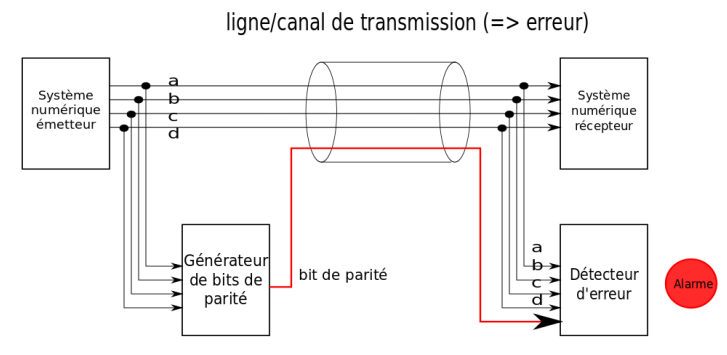
\includegraphics[scale=0.5]{./images/symb_7.png}
  \end{center}
\end{frame}

\begin{frame}{Codes détecteurs d'erreurs}
  \begin{center}
    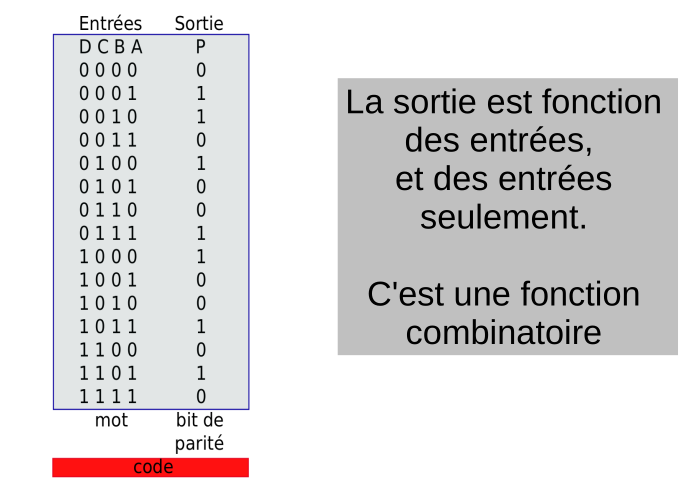
\includegraphics[scale=0.4]{./images/symb_8.png}
  \end{center}
\end{frame}

\begin{frame}{Claude Berrou et les turbocodes : correcteurs d'erreurs}

  \begin{columns}[c]
    \begin{column}{0.68\textwidth}
      \begin{block}{Une révolution née à Brest }
        \itshape
        En 1993, Claude Berrou et Alain Glavieux (ENST/IMT Atlantique) bouleversent la théorie
        de l'information en s'approchant de la \textbf{limite de Shannon},
        que les experts jugeaient inatteignable depuis 1948.
      \end{block}

      \vspace{0.3cm}
      \small
      Les \textbf{turbocodes} reposent sur un principe itératif :
      deux décodeurs élémentaires s'échangent des « croyances »
      jusqu'à converger vers le message original.

      \vspace{0.3cm}
      \textbf{Aujourd'hui :} 3G/4G, WiMAX, sondes spatiales
      (Mars Reconnaissance Orbiter, Messenger), plus de
      \textbf{4 milliards} de turbodécodeurs en circulation.
    \end{column}

    \begin{column}{0.28\textwidth}
      \centering
      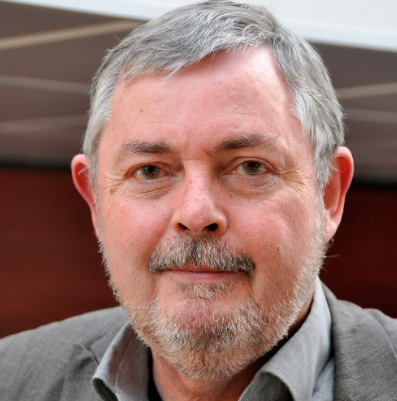
\includegraphics[scale=0.25]{./images/berrou.png}
      \vspace{0.2cm}
      {\scriptsize
        Claude Berrou (1951--)\\
        Télécom Bretagne\\
        Prix Marconi 2005\\
        Médaille Hamming 2003
      }
    \end{column}
  \end{columns}

\end{frame}


%========================================================================================
%\section*{Logique Booléenne et Combinatoire}
%========================================================================================
%

% =========================================================
\section{Algèbre de Boole}
% =========================================================

% --- Espace de Boole et variables ---
\begin{frame}{Espace de Boole et Variables Booléennes}

    \begin{block}{L'Espace de Boole \(\mathbb{B}\)}
        L'algèbre booléenne \footnote{L’algèbre de Boole est une algèbre au sens de structure algébrique, mais pas au sens d’algèbre sur un corps $\mathbb{K}$.} opère sur un ensemble à deux éléments :
        \[
            \mathbb{B} = \{0, 1\}
        \]
        où \(0\) représente \textbf{Faux} et \(1\) représente \textbf{Vrai}.
    \end{block}

    \vspace{0.4cm}

    \begin{columns}[T]
        \begin{column}{0.48\textwidth}
            \textbf{Variable booléenne simple}
            \begin{itemize}
                \item Une variable \(x\) qui ne peut prendre que deux valeurs.
                \item \(x \in \{0, 1\}\)
                \item Exemple : \textit{Un interrupteur est ouvert (0) ou fermé (1).}
            \end{itemize}
        \end{column}
        \begin{column}{0.48\textwidth}
            \textbf{Variable booléenne générale (vecteur)}
            \begin{itemize}
                \item Un vecteur de \(n\) bits : \(X = (x_{n-1}, \dots, x_0)\)
                \item \(X \in \mathbb{B}^n\)
                \item Exemple : \textit{Un octet (8 bits) représentant un état.}
            \end{itemize}
        \end{column}
    \end{columns}

\end{frame}

% --- Fonction booléenne ---
\begin{frame}{Fonction Booléenne}

    \begin{block}{Définition}
        Une \textbf{fonction booléenne} à \(n\) variables est une application :
        \[
            f : \mathbb{B}^n \to \mathbb{B}
        \]
        Elle associe à chaque combinaison d'entrées une unique sortie binaire.
    \end{block}

    \vspace{0.4cm}

    \begin{columns}[T]
        \begin{column}{0.55\textwidth}
            \textbf{Représentation}
            \begin{itemize}
                \item \textbf{Table de vérité} : énumère les \(2^n\) cas possibles.
                \item \textbf{Expression algébrique} : combinaison de \(+, \cdot, \bar{\phantom{x}}\).
            \end{itemize}

            \vspace{0.3cm}
            \textit{Exemple :} \(f(x,y) = x \cdot \bar{y} + \bar{x} \cdot y\) (XOR)
        \end{column}
        \begin{column}{0.4\textwidth}
            \centering
            \begin{tabular}{|c|c|c|}
                \hline
                \(x\) & \(y\) & \(f(x,y)\) \\
                \hline
                0 & 0 & 0 \\
                0 & 1 & 1 \\
                1 & 0 & 1 \\
                1 & 1 & 0 \\
                \hline
            \end{tabular}
        \end{column}
    \end{columns}

\end{frame}

% =========================================================
\section{Opérations}
% =========================================================

% --- Opérations fondamentales ---
\begin{frame}{Opérations Fondamentales}

    On utilise usuellement les symboles \(+\) pour le \textbf{OU} et \(\cdot\) (ou \(*\)) pour le \textbf{ET}.

    \vspace{0.3cm}

    \begin{columns}[T]
        \begin{column}{0.3\textwidth}
            \centering
            \textbf{Négation (NON)}\\
            \(\bar{x}\) ou \(\neg x\)
            \vspace{0.2cm}

            \begin{tabular}{|c|c|}
                \hline
                \(x\) & \(\bar{x}\) \\
                \hline
                0 & 1 \\
                1 & 0 \\
                \hline
            \end{tabular}
        \end{column}

        \begin{column}{0.35\textwidth}
            \centering
            \textbf{Conjonction (ET)}\\
            \(x \cdot y\) ou \(x * y\)
            \vspace{0.2cm}

            \begin{tabular}{|c|c|c|}
                \hline
                \(x\) & \(y\) & \(x \cdot y\) \\
                \hline
                0 & 0 & 0 \\
                0 & 1 & 0 \\
                1 & 0 & 0 \\
                1 & 1 & 1 \\
                \hline
            \end{tabular}
        \end{column}

        \begin{column}{0.35\textwidth}
            \centering
            \textbf{Disjonction (OU)}\\
            \(x + y\)
            \vspace{0.2cm}

            \begin{tabular}{|c|c|c|}
                \hline
                \(x\) & \(y\) & \(x + y\) \\
                \hline
                0 & 0 & 0 \\
                0 & 1 & 1 \\
                1 & 0 & 1 \\
                1 & 1 & 1 \\
                \hline
            \end{tabular}
        \end{column}
    \end{columns}

\end{frame}

% --- Opérateurs dérivés (aperçu) ---
\begin{frame}{Opérateurs Dérivés}

    Au-delà des trois opérations de base (\(+, \cdot, \bar{\phantom{x}}\)), on définit des \textbf{opérateurs dérivés} très utilisés en logique et en électronique.

    \vspace{0.4cm}

    \centering
    \begin{tabular}{|c|c|c|}
        \hline
        \textbf{Nom} & \textbf{Symbole} & \textbf{Expression en base} \\
        \hline
        OU exclusif (XOR) & \(x \oplus y\) & \(x \cdot \bar{y} + \bar{x} \cdot y\) \\
        NAND & \(x \uparrow y\) & \(\overline{x \cdot y}\) \\
        NOR & \(x \downarrow y\) & \(\overline{x + y}\) \\
        Équivalence (XNOR) & \(x \Leftrightarrow y\) & \(x \cdot y + \bar{x} \cdot \bar{y}\) \\
        Implication & \(x \Rightarrow y\) & \(\bar{x} + y\) \\
        \hline
    \end{tabular}

    \vspace{0.5cm}

    \begin{block}{Idée clé}
        Tous ces opérateurs se ramènent aux trois opérations fondamentales.
    \end{block}

\end{frame}

% --- XOR ---
\begin{frame}{Le OU Exclusif (\(x \oplus y\))}

    \begin{block}{Définition}
        « \(x\) ou \(y\), mais pas les deux » — noté \(x \oplus y\).
        \[
            x \oplus y \;=\; x \cdot \bar{y} + \bar{x} \cdot y
        \]
    \end{block}

    \vspace{0.4cm}

    \begin{columns}[T]
        \begin{column}{0.42\textwidth}
            \centering
            \begin{tabular}{|c|c|c|}
                \hline
                \(x\) & \(y\) & \(x \oplus y\) \\
                \hline
                0 & 0 & 0 \\
                0 & 1 & 1 \\
                1 & 0 & 1 \\
                1 & 1 & 0 \\
                \hline
            \end{tabular}
        \end{column}
        \begin{column}{0.55\textwidth}
            \textbf{Propriétés utiles :}
            \begin{itemize}
                \item \(x \oplus x = 0\)
                \item \(x \oplus \bar{x} = 1\)
                \item \(x \oplus 0 = x\)
                \item \(x \oplus 1 = \bar{x}\)
                \item \textbf{Associatif et commutatif}
            \end{itemize}

            \vspace{0.2cm}
            \textit{Application : addition binaire, détection de parité.}
        \end{column}
    \end{columns}

\end{frame}

% --- NAND et NOR ---
\begin{frame}{NAND et NOR : les Portes Universelles}

    \begin{columns}[T]
        \begin{column}{0.48\textwidth}
            \begin{block}{NAND (\(x \uparrow y\))}
                \[
                    x \uparrow y = \overline{x \cdot y}
                \]
                \centering
                \begin{tabular}{|c|c|c|}
                    \hline
                    \(x\) & \(y\) & \(x \uparrow y\) \\
                    \hline
                    0 & 0 & 1 \\
                    0 & 1 & 1 \\
                    1 & 0 & 1 \\
                    1 & 1 & 0 \\
                    \hline
                \end{tabular}
            \end{block}
        \end{column}

        \begin{column}{0.48\textwidth}
            \begin{block}{NOR (\(x \downarrow y\))}
                \[
                    x \downarrow y = \overline{x + y}
                \]
                \centering
                \begin{tabular}{|c|c|c|}
                    \hline
                    \(x\) & \(y\) & \(x \downarrow y\) \\
                    \hline
                    0 & 0 & 1 \\
                    0 & 1 & 0 \\
                    1 & 0 & 0 \\
                    1 & 1 & 0 \\
                    \hline
                \end{tabular}
            \end{block}
        \end{column}
    \end{columns}

    \vspace{0.4cm}

    \begin{alertblock}{Universalité}
        Toute fonction booléenne peut être réalisée en n'utilisant \textbf{que des NAND} ou \textbf{que des NOR}.
    \end{alertblock}

\end{frame}
% --- Équivalence ---
\begin{frame}{L'Équivalence (\(x \Leftrightarrow y\))}

    \begin{block}{Définition}
        « \(x\) si et seulement si \(y\) » — notée \(x \Leftrightarrow y\), également écrite \(x \leftrightarrow y\) ou XNOR.
        \[
            x \Leftrightarrow y \;=\; x \cdot y + \bar{x} \cdot \bar{y}
        \]
    \end{block}

    \vspace{0.4cm}

    \begin{columns}[T]
        \begin{column}{0.42\textwidth}
            \centering
            \begin{tabular}{|c|c|c|}
                \hline
                \(x\) & \(y\) & \(x \Leftrightarrow y\) \\
                \hline
                0 & 0 & 1 \\
                0 & 1 & 0 \\
                1 & 0 & 0 \\
                1 & 1 & 1 \\
                \hline
            \end{tabular}
        \end{column}
        \begin{column}{0.55\textwidth}
            \textbf{Points à retenir :}
            \begin{itemize}
                \item Vraie quand \(x\) et \(y\) sont \textbf{identiques}.
                \item C'est la \textbf{négation du XOR}.
                \item \(x \Leftrightarrow y = \overline{x \oplus y}\)
            \end{itemize}

            \vspace{0.3cm}
            \textit{Lien avec l'implication :}
            \[
                (x \Rightarrow y) \cdot (y \Rightarrow x) = x \Leftrightarrow y
            \]
        \end{column}
    \end{columns}

\end{frame}

% --- Implication : définition ---
\begin{frame}{L'Implication (\(x \Rightarrow y\)) : Définition}

    \begin{block}{Définition}
        « Si \(x\) alors \(y\) » — notée \(x \Rightarrow y\) ou \(x \to y\).
        \[
            x \Rightarrow y \;=\; \bar{x} + y
        \]
    \end{block}

    \vspace{0.4cm}

    \begin{columns}[T]
        \begin{column}{0.42\textwidth}
            \centering
            \begin{tabular}{|c|c|c|}
                \hline
                \(x\) & \(y\) & \(x \Rightarrow y\) \\
                \hline
                0 & 0 & 1 \\
                0 & 1 & 1 \\
                1 & 0 & \textbf{0} \\
                1 & 1 & 1 \\
                \hline
            \end{tabular}
        \end{column}
        \begin{column}{0.55\textwidth}
            \textbf{Un seul cas rend l'implication fausse :}
            \[
                x = 1 \quad \text{et} \quad y = 0
            \]

            \vspace{0.3cm}
            C'est le seul \textbf{contre-exemple} possible : l'antécédent est vrai mais la conclusion ne l'est pas.
        \end{column}
    \end{columns}

    \vspace{0.3cm}
    \centering
    \textit{Reformulation : \(x \Rightarrow y = \overline{x \cdot \bar{y}}\)\quad (négation d'un contre-exemple).}

\end{frame}

% --- Implication : paradoxe de l'antécédent faux ---
\begin{frame}{Implication : pourquoi est-elle vraie quand \(x = 0\) ?}

    \begin{alertblock}{La difficulté}
        Intuitivement, on se demande pourquoi \(0 \Rightarrow 0\) et \(0 \Rightarrow 1\) valent \(1\).
    \end{alertblock}

    \vspace{0.3cm}

    \textbf{Clé :} l'implication est une \textbf{contrainte conditionnelle}.

    \vspace{0.2cm}

    \[
        x \Rightarrow y \quad \text{signifie :} \quad \text{« \textbf{si} } x \text{ est vrai, \textbf{alors} } y \text{ doit être vrai. »}
    \]

    \vspace{0.3cm}

    \begin{itemize}
        \item Si \(x = 1\) : la contrainte s'applique. Il faut \(y = 1\), sinon elle est \textbf{violée}.
        \item Si \(x = 0\) : la contrainte \textbf{ne s'applique pas}. Elle n'est donc \textbf{pas violée}, donc elle est \textbf{vraie par défaut} (\textit{vacuité}).
    \end{itemize}

    \vspace{0.4cm}

    \begin{exampleblock}{Analogie météo}
        \textit{« S'il pleut, alors je prends mon parapluie. »}\\[0.2cm]
        Cette règle n'est \textbf{violée que dans un seul cas} : il pleut \textbf{et} je ne prends pas de parapluie.
    \end{exampleblock}

\end{frame}

% --- Implication : précaution d'usage + table météo ---
\begin{frame}[shrink=10] {Implication : Précaution d'Usage et Table Météo}

    \begin{alertblock}{Précaution d'usage}
        L'énoncé \textit{« S'il pleut, je prends mon parapluie »} doit être compris comme une \textbf{règle que je m'engage à suivre}, et non comme une \textbf{causalité physique}. De plus, il \textbf{ne dit rien} sur mon comportement quand il ne pleut pas.
    \end{alertblock}

    \vspace{0.1cm}

    \centering
    \renewcommand{\arraystretch}{1.3}
    \begin{tabular}{|c|c|c|l|}
        \hline
        \textbf{Il pleut} & \textbf{Parapluie} & \textbf{Règle} & \textbf{Interprétation} \\
        \(x\) & \(y\) & \(x \Rightarrow y\) & \\
        \hline
        1 & 1 & 1 & Règle respectée \\
        \textbf{1} & \textbf{0} & \textbf{0} & \textbf{Règle violée} \\
        0 & 1 & 1 & Pas de pluie — libre de mes choix \\
        0 & 0 & 1 & Pas de pluie — libre de mes choix \\
        \hline
    \end{tabular}

    \vspace{0.2cm}

    \begin{columns}[T]
        \begin{column}{0.48\textwidth}
            \textbf{Contraposition :}\\
            \(x \Rightarrow y \equiv \bar{y} \Rightarrow \bar{x}\)\\
            \textit{« Si je n'ai pas de parapluie,}\\
            \textit{alors il ne pleut pas. »}
        \end{column}
        \begin{column}{0.48\textwidth}
          \textbf{Identités remarquables :}
          \begin{align*}
            (0 \Rightarrow y) &= 1 \\
            (1 \Rightarrow y) &= y \\
            (x \Rightarrow 1) &= 1 \\
            (x \Rightarrow 0) &= \bar{x}
          \end{align*}
        \end{column}
    \end{columns}

\end{frame}

% --- Autres formes d'implication ---
\begin{frame}{Autres Formes d'Implication}

    \textbf{Règle de base :} \textit{« S'il pleut, je prends un parapluie. »} \quad (\(x \Rightarrow y\))

    \vspace{0.1cm}

    \begin{columns}[T]
        \begin{column}{0.45\textwidth}
            \begin{block}{Réciproque}
                \(y \Rightarrow x\)\\
                \textit{« Si je prends un parapluie, alors il pleut. »}\\
                \textbf{Non équivalente}.
            \end{block}

            \vspace{0.2cm}

            \begin{block}{Contraposée}
                \(\bar{y} \Rightarrow \bar{x}\)\\
                \textit{« Si je ne prends pas de parapluie, alors il ne pleut pas. »}\\
                \textbf{Équivalente} à la règle de base.
            \end{block}
        \end{column}
        \begin{column}{0.50\textwidth}
            \begin{block}{Réciproque de la contraposée}
                \(\bar{x} \Rightarrow \bar{y}\)\\
                \textit{« S'il ne pleut pas, je ne prends pas de parapluie. »}\\
                \textbf{Non équivalente}.
            \end{block}

            \vspace{0.2cm}

            \begin{block}{Équivalence}
                \((x \Rightarrow y) \cdot (y \Rightarrow x) = x \Leftrightarrow y\)\\
                \textit{« Je prends un parapluie si et seulement s'il pleut. »}
            \end{block}
        \end{column}
    \end{columns}

    \vspace{0.1cm}

    \begin{alertblock}{Piège classique}
        \centering
        \textbf{Confondre une implication avec sa réciproque est l'erreur logique la plus fréquente.}
    \end{alertblock}
\end{frame}


% --- Récapitulatif ---
\begin{frame}{Récapitulatif des Opérateurs Booléens}

    \centering
    \small
    \begin{tabular}{|c|c||c|c|c|c|c|c|}
        \hline
        \(x\) & \(y\) & \(\cdot\) & \(+\) & \(\oplus\) & \(\Leftrightarrow\) & \(\Rightarrow\) & \(\uparrow\) \\
        \hline
        0 & 0 & 0 & 0 & 0 & 1 & 1 & 1 \\
        0 & 1 & 0 & 1 & 1 & 0 & 1 & 1 \\
        1 & 0 & 0 & 1 & 1 & 0 & 0 & 1 \\
        1 & 1 & 1 & 1 & 0 & 1 & 1 & 0 \\
        \hline
    \end{tabular}

    \vspace{0.4cm}

    \begin{columns}[T]
        \begin{column}{0.48\textwidth}
            \textbf{Opérateurs de base :}
            \begin{itemize}
                \item ET (\(\cdot\)), OU (\(+\)), NON (\(\bar{\phantom{x}}\))
            \end{itemize}
        \end{column}
        \begin{column}{0.48\textwidth}
            \textbf{Opérateurs dérivés :}
            \begin{itemize}
                \item XOR, XNOR, implication, NAND, NOR
            \end{itemize}
        \end{column}
    \end{columns}

    \vspace{0.3cm}
    \centering
    \textit{16 fonctions booléennes à 2 variables existent  \footnote{Deux variables d'où 4 lignes et 2 choix pour \underline{chacune} des lignes : $2\times 2\times 2\times 2=2^4=16$}— celles-ci sont les plus utilisées.}

\end{frame}

% --- Priorité et parenthésage ---
\begin{frame}{Priorité des Opérations et Parenthésage}

    Comme en arithmétique, il existe un ordre de priorité implicite.

    \vspace{0.5cm}

    \begin{block}{Ordre de priorité (du plus fort au plus faible)}
        \begin{enumerate}
            \item \textbf{Négation} : \(\bar{x}\)
            \item \textbf{Conjonction} : \(x \cdot y\)
            \item \textbf{Disjonction} : \(x + y\)
        \end{enumerate}
    \end{block}

    \vspace{0.4cm}

    \textbf{Exemple :}
    \[
        \bar{x} \cdot y + z = \big((\bar{x}) \cdot y\big) + z
    \]

    \vspace{0.2cm}
    \centering
    \textit{En cas de doute, les parenthèses restent la meilleure amie du logicien.}

\end{frame}

% =========================================================
\section{Propriétés Algébriques}
% =========================================================

% --- Commutativité et associativité ---
\begin{frame}{Commutativité et Associativité}

    Les opérations \(+\) et \(\cdot\) possèdent des propriétés similaires à l'arithmétique classique.

    \vspace{0.4cm}

    \begin{block}{Commutativité}
        L'ordre des opérandes n'influence pas le résultat.
        \begin{align*}
            x + y &= y + x \\
            x \cdot y &= y \cdot x
        \end{align*}
    \end{block}

    \begin{block}{Associativité}
        L'ordre d'évaluation (groupement) n'influence pas le résultat.
        \begin{align*}
            (x + y) + z &= x + (y + z) \\
            (x \cdot y) \cdot z &= x \cdot (y \cdot z)
        \end{align*}
    \end{block}

\end{frame}

% --- Distributivité ---
\begin{frame}{Distributivité}

    \begin{alertblock}{Particularité de l'algèbre de Boole}
        Contrairement à l'arithmétique, le OU est distributif sur le ET \textbf{et réciproquement}.
    \end{alertblock}

    \vspace{0.4cm}

    \begin{columns}[T]
        \begin{column}{0.48\textwidth}
            \textbf{ET sur OU} (classique)
            \[
                x \cdot (y + z) = (x \cdot y) + (x \cdot z)
            \]
        \end{column}
        \begin{column}{0.48\textwidth}
            \textbf{OU sur ET} (surprenant !)
            \[
                x + (y \cdot z) = (x + y) \cdot (x + z)
            \]
        \end{column}
    \end{columns}

    \vspace{0.5cm}
    \centering
    \textit{Cette double distributivité est une signature de l'algèbre de Boole.}

\end{frame}

% =========================================================
\section{Théorèmes}
% =========================================================

% --- Théorèmes principaux ---
\begin{frame}{Théorèmes Principaux}

    Ces théorèmes permettent de simplifier les expressions logiques.

    \vspace{0.3cm}

    \begin{columns}[T]
        \begin{column}{0.48\textwidth}
            \textbf{Éléments Neutres}
            \begin{align*}
                x + 0 &= x \\
                x \cdot 1 &= x
            \end{align*}

            \vspace{0.2cm}

            \textbf{Éléments Absorbants}
            \begin{align*}
                x + 1 &= 1 \\
                x \cdot 0 &= 0
            \end{align*}
        \end{column}

        \begin{column}{0.48\textwidth}
            \textbf{Idempotence}
            \begin{align*}
                x + x &= x \\
                x \cdot x &= x
            \end{align*}

            \vspace{0.2cm}

            \textbf{Complémentation}
            \begin{align*}
                x + \bar{x} &= 1 \\
                x \cdot \bar{x} &= 0
            \end{align*}
        \end{column}
    \end{columns}

\end{frame}

% --- Absorption ---
\begin{frame}{Lois d'Absorption}

    \begin{block}{Définition}
        L'absorption permet d'éliminer des termes redondants dans une expression.
    \end{block}

    \vspace{0.5cm}

    \begin{columns}[T]
        \begin{column}{0.48\textwidth}
            \begin{align*}
                x + x \cdot y &= ? \\
                x \cdot (1 + y) &= x
            \end{align*}
        \end{column}
        \begin{column}{0.48\textwidth}
            \centering
            \textit{Intuition :}\\
            \vspace{0.2cm}
            Si \(x\) est vrai, l'expression est vraie\\
            quel que soit \(y\).
        \end{column}
    \end{columns}

    \vspace{0.5cm}

    \begin{exampleblock}{Exemple d'application}
        \[
            x + x \cdot y + x \cdot z = x \cdot (1 + y + z) = x
        \]
    \end{exampleblock}

\end{frame}

% --- Dualité ---
\begin{frame}{Principe de Dualité}

    \begin{alertblock}{Principe}
        Toute identité booléenne reste vraie si l'on échange simultanément :
        \[
            + \longleftrightarrow \cdot \qquad \text{et} \qquad 0 \longleftrightarrow 1
        \]
    \end{alertblock}

    \vspace{0.4cm}

    \textbf{Cela explique pourquoi les théorèmes vont souvent par paires :}

    \vspace{0.3cm}

    \centering
    \begin{tabular}{|c|c|}
        \hline
        \textbf{Identité} & \textbf{Identité duale} \\
        \hline
        \(x + 0 = x\) & \(x \cdot 1 = x\) \\
        \(x + 1 = 1\) & \(x \cdot 0 = 0\) \\
        \(x + x = x\) & \(x \cdot x = x\) \\
        \(\overline{x + y} = \bar{x} \cdot \bar{y}\) & \(\overline{x \cdot y} = \bar{x} + \bar{y}\) \\
        \hline
    \end{tabular}

\end{frame}

% --- De Morgan ---
\begin{frame}{Lois de De Morgan}

    Ces lois sont fondamentales pour la manipulation des expressions booléennes et la conception de circuits logiques.

    \vspace{0.4cm}

    \begin{alertblock}{Première Loi de De Morgan}
        La négation d'une disjonction est la conjonction des négations.
        \[
            \overline{x + y} = \bar{x} \cdot \bar{y}
        \]
    \end{alertblock}

    \vspace{0.2cm}

    \begin{alertblock}{Deuxième Loi de De Morgan}
        La négation d'une conjonction est la disjonction des négations.
        \[
            \overline{x \cdot y} = \bar{x} + \bar{y}
        \]
    \end{alertblock}

    \vspace{0.2cm}
    \centering
    \textit{En résumé : l'inverse d'une somme n'est pas la somme des inverses, mais le produit des inverses.}

\end{frame}
% =========================================================
\section{Application}
% =========================================================

% --- Exemple fil rouge : vote majoritaire ---
\begin{frame}{Exemple : Vote Majoritaire à 3 Personnes}

    \textbf{Énoncé :} Trois personnes votent. La décision est adoptée si \textbf{au moins deux} votent OUI.

    \vspace{0.4cm}

    \begin{columns}[T]
        \begin{column}{0.45\textwidth}
            \textbf{Variables :} \(a, b, c \in \{0,1\}\) (1 = OUI).

            \vspace{0.3cm}
            \textbf{Forme SOP (lignes où \(f=1\)) :}
            \[
                f = \bar{a}bc + a\bar{b}c + ab\bar{c} + abc
            \]
        \end{column}
        \begin{column}{0.5\textwidth}
            \centering
            \begin{tabular}{|c|c|c|c|}
                \hline
                \(a\) & \(b\) & \(c\) & \(f\) \\
                \hline
                0 & 0 & 0 & 0 \\
                0 & 0 & 1 & 0 \\
                0 & 1 & 0 & 0 \\
                0 & 1 & 1 & 1 \\
                1 & 0 & 0 & 0 \\
                1 & 0 & 1 & 1 \\
                1 & 1 & 0 & 1 \\
                1 & 1 & 1 & 1 \\
                \hline
            \end{tabular}
        \end{column}
    \end{columns}

\end{frame}

% --- Simplification de l'exemple ---
\begin{frame}{Simplification par les Théorèmes}

    \textbf{Expression initiale (SOP) :}
    \[
        f = \bar{a}bc + a\bar{b}c + ab\bar{c} + abc
    \]

    \vspace{0.3cm}

    \textbf{Étape 1 — Idempotence} (on duplique \(abc\)) :
    \[
        f = \bar{a}bc + a\bar{b}c + ab\bar{c} + abc + abc
    \]

    \vspace{0.2cm}

    \textbf{Étape 2 — Regroupement} :
    \[
        f = (\bar{a}bc + abc) + (a\bar{b}c + abc) + (ab\bar{c} + abc)
    \]

    \vspace{0.2cm}

    \textbf{Étape 3 — Distributivité} (\(x \cdot y + x \cdot \bar{y} = x\)) :
    \[
        f = bc + ac + ab
    \]

    \vspace{0.1cm}

    \begin{exampleblock}{Résultat : $f = ab + ac + bc$}
        % \[
        %     f = ab + ac + bc
        % \]
        Forme simplifiée bien plus économique à implémenter.
    \end{exampleblock}

\end{frame}

% --- Transition vers les circuits ---

% =========================================================
\section{Décomposition de Shannon et Formes Canoniques}
% =========================================================
% --- Frame : Décomposition de Shannon ---
\begin{frame}{Décomposition de Shannon}

    \begin{block}{Théorème — Expansion de Shannon }
        Toute fonction booléenne \(f : \mathbb{B}^n \to \mathbb{B}\) peut être décomposée par rapport à une variable \(x_i\) :
        \[
            f(\dots, x_i, \dots) = x_i \cdot f_{x_i=1} + \bar{x_i} \cdot f_{x_i=0}
        \]
        où \(f_{x_i=1}\) et \(f_{x_i=0}\) sont les \textbf{cofacteurs} de \(f\) par rapport à \(x_i\).
    \end{block}

    \vspace{0.1cm}

    \begin{columns}[T]
        \begin{column}{0.52\textwidth}
            \textbf{Forme duale (par rapport à \(+\)) :}
            \[
                f = (x_i + f_{x_i=0}) \cdot (\bar{x_i} + f_{x_i=1})
            \]

            \vspace{0.1cm}

            \textbf{Interprétation :}
            \begin{itemize}
                \item On \textbf{factorise} par \(x_i\).
                \item On évalue \(f\) dans les deux cas \(x_i = 1\) et \(x_i = 0\).
                \item Chaque cofacteur a une variable en moins.
                \item \texttt{BDD} en CAO : \textit{binary decision diagrams}.
            \end{itemize}
        \end{column}

        \begin{column}{0.45\textwidth}
            \begin{exampleblock}{Exemple : XOR}
                \(f(x,y) = x \oplus y \)

                \vspace{0.1cm}

                Décomposition par rapport à \(x\) :
                \begin{align*}
                    f_{x=1} &= \bar{y} \\
                    f_{x=0} &= y
                \end{align*}
                \[
                    f = x \cdot \bar{y} + \bar{x} \cdot y
                \]
            \end{exampleblock}
        \end{column}
    \end{columns}


\end{frame}

%\end{document}
% --- SOP / POS ---
\begin{frame}{Formes Canoniques : SOP et POS}

    \begin{columns}[T]
        \begin{column}{0.48\textwidth}
            \begin{block}{SOP (\textit{Sum of Products})}
                Somme de \textbf{mintermes} (produits où chaque variable apparaît une fois).
                \[
                    f = \bar{x} \cdot y + x \cdot \bar{y}
                \]
                Construite à partir des lignes où \(f = 1\).
            \end{block}
        \end{column}
        \begin{column}{0.48\textwidth}
            \begin{block}{POS (\textit{Product of Sums})}
                Produit de \textbf{maxtermes} (sommes où chaque variable apparaît une fois).
                \[
                    f = (x + y) \cdot (\bar{x} + \bar{y})
                \]
                Construite à partir des lignes où \(f = 0\).
            \end{block}
        \end{column}
    \end{columns}

    \vspace{0.5cm}

    \begin{exampleblock}{Lien avec la table de vérité}
        Toute fonction booléenne admet une unique forme canonique SOP et une unique forme canonique POS.
    \end{exampleblock}

\end{frame}

% =========================================================
\section{Tableau de Karnaugh}
% =========================================================
\begin{frame}{Tableau de Karnaugh : intuition}
  \begin{columns}
    \begin{column}{0.3\textwidth}
      \begin{itemize}
        \item \textbf{objectif} : simplifier une formule booléenne.
        \item \textbf{moyen} : disposition spatiale \textit{particulière}.
      \end{itemize}
    \end{column}
    \begin{column}{0.7\textwidth}
      \begin{center}
        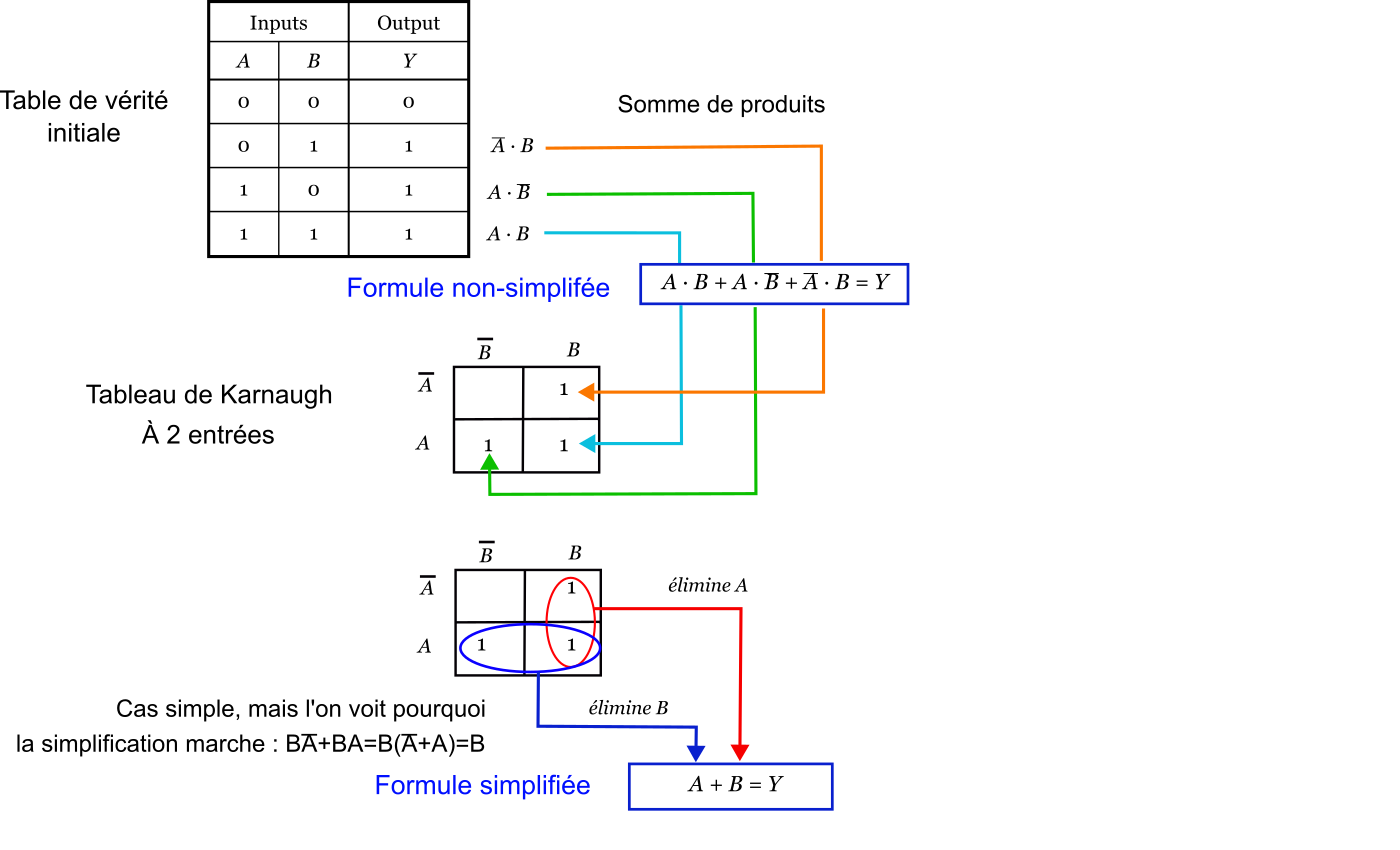
\includegraphics[scale=0.32]{./images/karnaugh_0.png}
      \end{center}
    \end{column}
  \end{columns}
\end{frame}

% --- Karnaugh : adjacence et principe ---
\begin{frame}{Tableau de Karnaugh : Adjacence et Principe}

    \begin{block}{Distance de Hamming}
        Pour deux vecteurs booléens \(u, v \in \mathbb{B}^n\), on définit :
        \[
            d_H(u,v) = \big|\{ i \in \{0,\dots,n-1\} : u_i \neq v_i \}\big|
        \]
        C'est le nombre de bits qui diffèrent entre \(u\) et \(v\).
    \end{block}

    \vspace{0.2cm}

    \begin{alertblock}{Définition — Adjacence}
        Deux cases du tableau de Karnaugh sont dites \textbf{adjacentes} si et seulement si : $d_H(u, v) = 1$
        % \[
        %     d_H(u, v) = 1
        % \]
        c'est-à-dire qu'elles ne diffèrent que par \textbf{une seule variable}.
    \end{alertblock}

    \vspace{0.1cm}

    \begin{columns}[T]
        \begin{column}{0.5\textwidth}
            \textbf{Justification :} si deux cases adjacentes ne diffèrent que par \(x\), leurs mintermes sont \(x \cdot m\) et \(\bar{x} \cdot m\), et :
            \[
                x \cdot m + \bar{x} \cdot m = (x + \bar{x}) \cdot m = m
            \]
            La variable \(x\) \textbf{disparaît}.
        \end{column}
        \begin{column}{0.45\textwidth}
            \textbf{Conséquence topologique :}\\
            Le tableau est \textbf{torique} — les bords opposés sont adjacents.

            \vspace{0.2cm}
            \textit{Exemple : \(000\) et \(100\) sont adjacents (\(d_H = 1\)).}
        \end{column}
    \end{columns}

\end{frame}

% --- Karnaugh : construction + code de Gray ---
\begin{frame}{Tableau de Karnaugh : Construction et Code de Gray}

    \begin{block}{Problème}
        Sur un tableau ordonné en binaire naturel, les cases voisines ne sont pas nécessairement adjacentes au sens de Hamming.
    \end{block}

    \vspace{0.3cm}

    \begin{columns}[T]
        \begin{column}{0.5\textwidth}
            \begin{alertblock}{Solution : Code de Gray}
                Ordonner les lignes et colonnes selon la suite :
                \[
                    00 \to 01 \to 11 \to 10
                \]
                Deux entrées consécutives diffèrent d'\textbf{un seul bit} (\(d_H = 1\)).
            \end{alertblock}
        \end{column}
        \begin{column}{0.45\textwidth}
            \centering
            \renewcommand{\arraystretch}{1.4}
            \begin{tabular}{|c|c|c|c|c|}
                \hline
                \(a \backslash bc\) & \(00\) & \(01\) & \textbf{\(11\)} & \(10\) \\
                \hline
                \(0\) & ~ & ~ & ~ & ~ \\
                \hline
                \(1\) & ~ & ~ & ~ & ~ \\
                \hline
            \end{tabular}
            % \begin{tabular}{|c|c|c|}
            %     \hline
            %     \(x \backslash y\) & \(0\) & \(1\) \\
            %     \hline
            %     \(0\) & \(\bar{x}\bar{y}\) & \(\bar{x}y\) \\
            %     \hline
            %     \(1\) & \(x\bar{y}\) & \(xy\) \\
            %     \hline
            % \end{tabular}

            \vspace{0.3cm}
            \textit{Chaque case = un minterme.}
        \end{column}
    \end{columns}

    \vspace{0.3cm}

    \textbf{Vérification :} \(00\) et \(01\) sont adjacents, \(01\) et \(11\) aussi, et ainsi de suite. La suite Gray garantit que toutes les cases voisines du tableau sont adjacentes au sens de Hamming.

\end{frame}

% --- Karnaugh : exemple 3 variables ---
\begin{frame}{Exemple : Tableau de Karnaugh à 3 Variables}

    \textbf{Fonction :} \(f(a,b,c) = \sum m(1,3,5,7)\)

    \vspace{0.3cm}

    \begin{columns}[T]
        \begin{column}{0.5\textwidth}
            \centering
            \renewcommand{\arraystretch}{1.6}
            \begin{tabular}{|c|c|c|c|c|}
                \hline
                \(a \backslash bc\) & \(00\) & \(01\) & \(11\) & \(10\) \\
                \hline
                \(0\) & 0 & \textbf{1} & \textbf{1} & 0 \\
                \hline
                \(1\) & 0 & \textbf{1} & \textbf{1} & 0 \\
                \hline
            \end{tabular}

            \vspace{0.3cm}

            \textit{Colonnes en code Gray : \(00, 01, 11, 10\).}
        \end{column}
        \begin{column}{0.48\textwidth}
            \textbf{Résolution :}

            \vspace{0.3cm}

            \begin{itemize}
                \item On regroupe les 4 \textbf{1} en un bloc \(2 \times 2\).
                \item Variables qui \textbf{changent} : \(a\) et \(b\).
                \item Variable qui \textbf{reste} : \(c = 1\).
                \item {\color{red} (Erreur dans le slideware distribué).} 
            \end{itemize}

            \vspace{0.4cm}

            \begin{exampleblock}{Résultat}
                \[
                    f = c
                \]
                De 4 mintermes à un seul littéral.
            \end{exampleblock}
        \end{column}
    \end{columns}


\end{frame}

% --- Karnaugh : regroupements formels ---
\begin{frame}{Regroupements : Règles Formelles}

    \begin{block}{Regroupement valide}
        Un regroupement est un sous-ensemble \(S\) de cases contenant des 1, tel que :
        \begin{itemize}
            \item \(|S| = 2^k\) pour un certain \(k \in \mathbb{N}\) ;
            \item \(S\) forme un \textbf{sous-cube} : produit cartésien de \(k\) paires d'entrées adjacentes.
        \end{itemize}
    \end{block}

    \vspace{0.3cm}

    \begin{alertblock}{Interprétation}
        Un sous-cube de taille \(2^k\) correspond à l'élimination de \(k\) variables par adjacence successive.
    \end{alertblock}

    \vspace{0.3cm}

    \begin{columns}[T]
        \begin{column}{0.5\textwidth}
            \textbf{Démarche :}
            \begin{enumerate}
                \item Remplir le tableau depuis la table de vérité.
                \item Identifier les \textbf{plus grands sous-cubes}.
                \item Vérifier que tous les 1 sont couverts.
                \item Lire le terme associé à chaque sous-cube.
            \end{enumerate}
        \end{column}
        \begin{column}{0.45\textwidth}
            \begin{exampleblock}{Limites}
                \begin{itemize}
                    \item Pratique jusqu'à 4 variables.
                    \item Difficile dès 5.
                    \item Au-delà : \textbf{Quine-McCluskey} ou \textbf{BDD}.
                \end{itemize}
            \end{exampleblock}
        \end{column}
    \end{columns}
\end{frame}

%\section{Du booléen au circuit}

\begin{frame}{Portes élémentaires}

    Chaque opération booléenne correspond à une \textbf{porte logique} physique, \textit{pour peu qu'elle ait été conçue par le fondeur} (au niveau transistor).

    \vspace{0.5cm}

    \centering
    \begin{tabular}{|c|c|c|}
        \hline
        \textbf{Opération} & \textbf{Symbole} & \textbf{Porte logique} \\
        \hline
        Négation & \(\bar{x}\) & NOT \\
        Conjonction & \(x \cdot y\) & AND2 \\
        Disjonction & \(x + y\) & OR2 \\
        Disjonction & \(x + y + z\) & OR3 \\

        \hline
    \end{tabular}

    \vspace{0.6cm}

    \begin{block}{Portes universelles}
        Les portes \textbf{NAND} et \textbf{NOR} sont dites \textit{universelles} : toute fonction booléenne peut être réalisée à partir de l'une d'elles uniquement.
    \end{block}

    \vspace{0.3cm}
    \centering
    \textit{L'algèbre de Boole est le langage mathématique de l'électronique numérique.}

\end{frame}



\begin{frame}{Portes logiques : symboles usuels}
  \begin{center}
    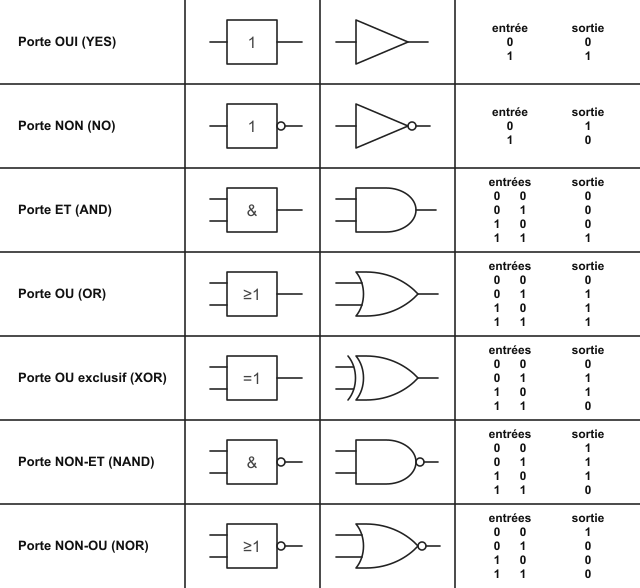
\includegraphics[scale=0.45]{./images/portes_logiques.png}
  \end{center}
\end{frame}


\begin{frame}{Portes Logiques : du Booléen au Modèle Physique}

    %\vspace{0.3cm}

    \begin{columns}[T]
        \begin{column}{0.52\textwidth}
          \begin{block}{Définition  (tentative) — Porte logique }
            Une \textbf{porte logique} à \(k\) entrées est un triplet :
            \[
            g = (f_g, \tau_g, A_g)
            \]
            où :
            \begin{itemize}
              \item \(f_g : \mathbb{B}^k \to \mathbb{B}\) est la \textbf{fonction réalisée} ;
              \item \(\tau_g \geq 0\) est le \textbf{délai de propagation} (temps) ;
              \item \(A_g \geq 0\) est la \textbf{surface} occupée (espace).
            \end{itemize}
          \end{block}
            \textbf{Modèle d'un circuit combinatoire}\\[0.2cm]
            Un circuit est un \textbf{graphe orienté acyclique} (DAG) :
            \[
                G = (V, E)
            \]
            \begin{itemize}
                \item \(V\) : portes \(\cup\) entrées \(\cup\) sorties ;
                \item \(E \subseteq V \times V\) : fils (connexions).
            \end{itemize}

            \vspace{0.2cm}
            La fonction globale \(F : \mathbb{B}^n \to \mathbb{B}^m\) est obtenue par \textbf{composition} le long du DAG.
        \end{column}
        \begin{column}{0.45\textwidth}
            \centering
            \renewcommand{\arraystretch}{1.2}
            \begin{tabular}{|c|c|c|c|}
                \hline
                \textbf{Porte} & \textbf{Fonction} & \(A\) (µm²) & \(\tau\) (ns) \\
                \hline
                INV   & \(\bar{a}\)            & 1 & 0.05 \\
                NAND2 & \(\overline{ab}\)      & 2 & 0.08 \\
                NOR2  & \(\overline{a+b}\)     & 2 & 0.09 \\
                AND2  & \(ab\)                 & 3 & 0.13 \\
                OR2   & \(a+b\)                & 3 & 0.14 \\
                XOR2  & \(a \oplus b\)         & 6 & 0.22 \\
                \hline
            \end{tabular}
            \vspace{0.2cm}

            {\footnotesize Chiffres indicatifs (nœud technologique générique).}

            \begin{alertblock}{Circuit Combinatoire}
              Pas de cycle = pas de rebouclage.
            \end{alertblock}
        \end{column}
    \end{columns}

    \vspace{0.2cm}

    \begin{alertblock}{Rupture conceptuelle}
        \centering
        On passe d'une fonction \textbf{intemporelle} \(f : \mathbb{B}^n \to \mathbb{B}\) à un objet \textbf{coûteux} : chaque porte a un prix en temps et en surface.
    \end{alertblock}

\end{frame}
%
% % --- Frame : Netlist et hiérarchie ---
% \begin{frame}{Netlist et Hiérarchie : la Structure Formelle d'un Circuit}
%
%     \begin{block}{Définition — Netlist}
%         Une \textbf{netlist} est un triplet :
%         \[
%             \mathcal{N} = (V, N, \pi)
%         \]
%         où :
%         \begin{itemize}
%             \item \(V\) est un ensemble d'\textbf{instances} de cellules ;
%             \item \(N\) est un ensemble de \textbf{nets} (fils) ;
%             \item \(\pi : V \to N^*\) associe à chaque instance ses ports connectés.
%         \end{itemize}
%     \end{block}
%
%     \vspace{0.3cm}
%
%     \begin{columns}[T]
%         \begin{column}{0.5\textwidth}
%             \begin{alertblock}{Définition — Module hiérarchique}
%                 Un \textbf{module} est un couple :
%                 \[
%                     M = (\text{ports},\, \text{implémentation})
%                 \]
%                 où l'implémentation est elle-même une netlist (récursion).
%             \end{alertblock}
%
%             \vspace{0.2cm}
%
%             \textbf{Encapsulation :} l'interface (ports) cache l'implémentation.\\
%             \textit{Principe de boîte noire :}\\
%             \[
%                 M : \mathbb{B}^{p} \to \mathbb{B}^{q}
%             \]
%         \end{column}
%         \begin{column}{0.48\textwidth}
%             \textbf{Exemple — Additionneur 8 bits :}
%
%             \vspace{0.3cm}
%
%             \centering
%             \begin{tikzpicture}[
%                 scale=0.7,
%                 every node/.style={draw, rounded corners, minimum height=0.6cm, font=\footnotesize}
%             ]
%                 \node (top) at (0, 2.5) {Top};
%                 \node (add8) at (0, 1.5) {Adder8};
%                 \node (a4a) at (-1.6, 0.4) {Adder4};
%                 \node (a4b) at (1.6, 0.4) {Adder4};
%                 \node (fa1) at (-2.4, -0.7) {FA};
%                 \node (fa2) at (-1.0, -0.7) {FA};
%                 \node (fa3) at (0.8, -0.7) {FA};
%                 \node (fa4) at (2.2, -0.7) {FA};
%
%                 \draw (top) -- (add8);
%                 \draw (add8) -- (a4a);
%                 \draw (add8) -- (a4b);
%                 \draw (a4a) -- (fa1);
%                 \draw (a4a) -- (fa2);
%                 \draw (a4b) -- (fa3);
%                 \draw (a4b) -- (fa4);
%             \end{tikzpicture}
%         \end{column}
%     \end{columns}
%
%     \vspace{0.2cm}
%
%     \begin{exampleblock}{Instanciation et réutilisation}
%         \centering
%         \(\text{Adder8} = \text{Adder4} \circ \text{Adder4}\) — la composition de modules préserve la fonction et divise la complexité.
%     \end{exampleblock}
%
% \end{frame}
%
% % --- Frame : Chemin critique et fréquence ---
% \begin{frame}{Chemin Critique et Fréquence de Fonctionnement}
%
%     \begin{block}{Modèle temporel}
%         À chaque porte \(v \in V\), on associe un délai \(\tau_v \geq 0\).
%
%         Le \textbf{délai d'un chemin} \(P = (v_0, v_1, \dots, v_k)\) est :
%         \[
%             T(P) \;=\; \sum_{i=0}^{k} \tau_{v_i}
%         \]
%     \end{block}
%
%     \vspace{0.3cm}
%
%     \begin{alertblock}{Définition — Chemin critique}
%         Le \textbf{chemin critique} est le chemin de délai maximal entre une entrée et une sortie :
%         \[
%             T_{\text{crit}} \;=\; \max_{P \in \mathcal{P}} \; T(P)
%         \]
%         où \(\mathcal{P}\) désigne l'ensemble des chemins entrée \(\to\) sortie.
%     \end{alertblock}
%
%     \vspace{0.3cm}
%
%     \begin{columns}[T]
%         \begin{column}{0.52\textwidth}
%             \textbf{Fréquence maximale} (modèle combinatoire pur) :
%             \[
%                 f_{\max} \;=\; \frac{1}{T_{\text{crit}}}
%             \]
%
%             \vspace{0.3cm}
%
%             \textbf{Slack} d'un chemin \(P\) :
%             \[
%                 s(P) \;=\; T_{\text{requis}} - T(P)
%             \]
%             \begin{itemize}
%                 \item \(s(P) = 0\) : chemin critique ;
%                 \item \(s(P) > 0\) : marge disponible.
%             \end{itemize}
%         \end{column}
%         \begin{column}{0.45\textwidth}
%             \begin{exampleblock}{Interprétation algorithmique}
%                 Le calcul de \(T_{\text{crit}}\) se fait en \(O(|V| + |E|)\) par :
%                 \begin{enumerate}
%                     \item tri topologique du DAG ;
%                     \item propagation des délais en avant (plus long chemin).
%                 \end{enumerate}
%
%                 \vspace{0.2cm}
%                 C'est un \textbf{plus long chemin dans un DAG} — problème classique de théorie des graphes.
%             \end{exampleblock}
%         \end{column}
%     \end{columns}
%
%     \vspace{0.2cm}
%
%     \begin{block}{Problème d'optimisation temporelle}
%         \centering
%         Maximiser le \textbf{slack minimum} sous contrainte de préservation de la fonction :
%         \[
%             \max_{G'} \; \min_{P} \; s(P) \quad \text{s.c.} \quad F_{G'} = F_{G}, \quad A_{G'} \leq A_{\max}
%         \]
%     \end{block}
%
% \end{frame}

\begin{frame}
\frametitle{Mapping technologique : de l'équation booléenne à la structure}

\vspace{0.2cm}

\begin{center}
\begin{tikzpicture}[
    node distance=1.6cm,
    box/.style={draw=black!70, rounded corners=2pt,
                minimum width=3.6cm, minimum height=1.1cm,
                align=center, font=\small},
    arr/.style={-{Latex[length=2.5mm]}, thick, black!70}
]

\node[box] (eq) {\textbf{Équations booléennes}\\[2pt]
                  $f = \overline{a}\,b + c\,(\overline{a} + d)$};

\node[box, right=of eq] (lib) {\textbf{Bibliothèque fondeur}\\[2pt]
                  \texttt{AND2, OR2, INV, NAND2, \dots}};

\node[box, right=of lib] (net) {\textbf{Structure effective}\\[2pt]
                  netlist / layout};

\draw[arr] (eq) -- node[above, font=\scriptsize]{simplification}
                 node[below, font=\scriptsize]{Mapping} (lib);
\draw[arr] (lib) -- node[above, font=\scriptsize]{connexion} (net);

\end{tikzpicture}
\end{center}

\vspace{0.35cm}

\begin{columns}[T]
\begin{column}{0.48\textwidth}
\textbf{Entrées du mapping}
\begin{itemize}\setlength\itemsep{2pt}
    \item Équations booléennes optimisées
    \item Bibliothèque de cellules (\emph{std cells})
    \item Reformulation selon disponibilité des cellules.
    \item Contraintes : aire, délai, fanout
\end{itemize}
\end{column}

\begin{column}{0.48\textwidth}
\textbf{Sortie effective}
\begin{itemize}\setlength\itemsep{2pt}
    \item Réseau de cellules interconnectées
    \item Respect des \emph{design rules}
    \item Prêt pour placement/routage
\end{itemize}
\end{column}
\end{columns}

\vfill
\begin{center}
\footnotesize\itshape
Le mapping traduit une expression logique en une réalisation physique contrainte par la bibliothèque du fondeur.
\end{center}

\end{frame}

% --- Frame : Porte, ports, instance ---
\begin{frame}{Circuit : tentative de définition formelle}

    \begin{block}{Définition — Port}
        Un \textbf{port} est un objet typé :
        \[
            p = (\text{nom},\, \text{direction},\, \text{largeur})
        \]
        avec \(\text{direction} \in \{in, out\}\) et \(\text{largeur} \in \mathbb{N}^*\).
    \end{block}

    \vspace{0.2cm}

    \begin{block}{Définition — Circuit (combinatoire)}
        Un \textbf{circuit} combinatoire est la donnée : $g = (\text{name},\, P_g,\, f_g,\, \tau_g,\, A_g)$
        % \[
        %     g = (\text{name},\, P_g,\, f_g,\, \tau_g,\, A_g)
        % \]
        où :
        \begin{itemize}
            \item \(P_g = P_g^{in} \uplus P_g^{out}\) : ensemble de ports, partitionné en entrées / sorties ;
            \item \(f_g : \mathbb{B}^{|P_g^{in}|} \to \mathbb{B}^{|P_g^{out}|}\) : fonction booléenne générale;
            \item \(\tau_g \in \mathbb{R}_{\geq 0}\) : délai caractéristique ;
            \item \(A_g \in \mathbb{R}_{\geq 0}\) : surface.
        \end{itemize}
    \end{block}

    % \vspace{0.1cm}
    %
    % \begin{columns}[T]
    %     \begin{column}{0.55\textwidth}
    %         \begin{alertblock}{Exemple — NAND2}
    %             \(P_g^{in} = \{a, b\}\), \; \(P_g^{out} = \{y\}\)\\[0.2cm]
    %             \(f_g(a,b) = \overline{a \cdot b}\), \quad \(\tau_g = 0.08\) ns, \quad \(A_g = 2\) µm²
    %         \end{alertblock}
    %     \end{column}
    %     \begin{column}{0.42\textwidth}
    %         \centering
    %         \begin{tabular}{|c|c|c|c|}
    %             \hline
    %             \textbf{Porte} & \(\tau\) (ns) & \(A\) (µm²) & Ports \\
    %             \hline
    %             INV   & 0.05 & 1 & \(\{a\} / \{y\}\) \\
    %             NAND2 & 0.08 & 2 & \(\{a,b\} / \{y\}\) \\
    %             NOR2  & 0.09 & 2 & \(\{a,b\} / \{y\}\) \\
    %             XOR2  & 0.22 & 6 & \(\{a,b\} / \{y\}\) \\
    %             \hline
    %         \end{tabular}
    %     \end{column}
    % \end{columns}

\end{frame}

% --- Frame : Netlist comme interconnexion de ports ---
\begin{frame}{Netlist : Interconnexion de Ports}

    \begin{block}{Définition — Instance de circuit}
        Une \textbf{instance} d'un circuit \(c\) \textbf{modèle} est un triplet :
        \[
            i = (c,\, \text{id},\, \sigma_i)
        \]
        où \(\sigma_i : P_c \to N\) associe chaque port de \(c\) à un \textbf{net} (\textit{fil}, \textit{wire}).

        Les ports de l'instance sont notés : \(\text{Ports}(i) = \{(i,p) \mid p \in P_c\}\).
    \end{block}

    \vspace{0.1cm}

    \begin{alertblock}{Définition — Netlist}
        Une \textbf{netlist} est un quadruplet $\mathcal{N} = (I,\, N,\, \Sigma,\, \text{io})$
        % \[
        %     \mathcal{N} = (I,\, N,\, \Sigma,\, \text{io})
        % \]
        où :
        \begin{itemize}
            \item \(I\) : ensemble d'instances ;
            \item \(N\) : ensemble de nets ;
            \item \(\Sigma = \{\sigma_i\}_{i \in I}\) : connexions port \(\to\) net ;
            \item \(\text{io}\) : ports externes de l'interface.
        \end{itemize}
    \end{alertblock}

\end{frame}



\begin{frame}{Exemple : netlist élémentaire}
  \begin{center}
    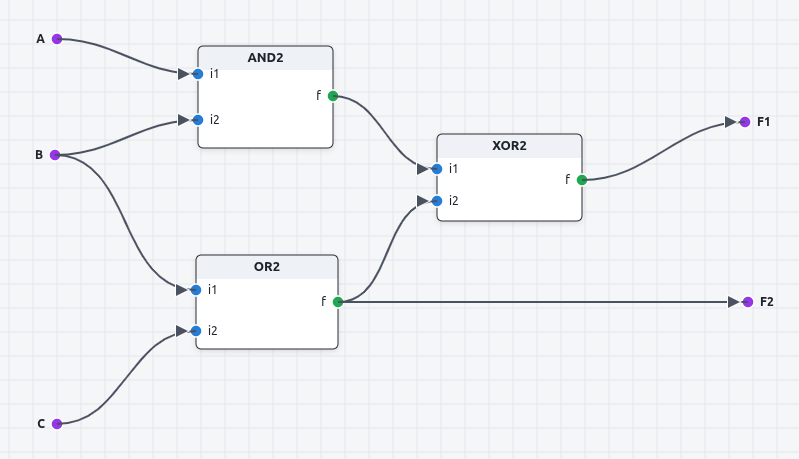
\includegraphics[scale=0.3]{./images/netlist_1.png}
  \end{center}
  Notes :
  \begin{itemize}
    \item partage de ressources (ici \texttt{OR2}) entre 2 fonctions $F1$ et $F2$
  \end{itemize}
\end{frame}

\begin{frame}{Exemple : introduction de hiérarchie}
  \begin{center}
    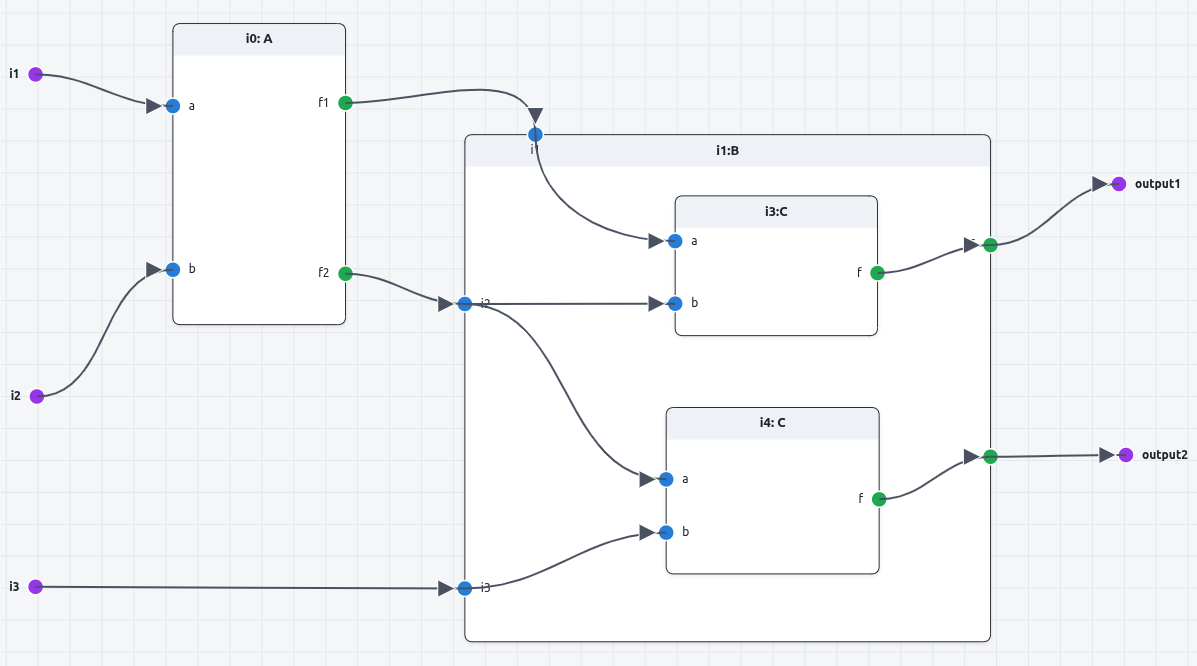
\includegraphics[scale=0.25]{./images/netlist_2.png}
  \end{center}
  Notes :
  \begin{itemize}
    \item \texttt{i3} et \texttt{i4} sont des \textit{instance} d'un modèle composant (modèle) \texttt{C}.
  \end{itemize}
\end{frame}

\begin{frame}{Compléments : signaux directionnels et encapsulation}
  \begin{columns}[T]
    \begin{column}{0.55\textwidth}
      \textbf{Signaux \textit{pilotés} :}
      \begin{enumerate}
        \item \textbf{Connexion} : tout net est piloté par un port (\textit{driver}).
        \item \textbf{Fanout} : un port pilote un ou plusieurs nets.
        \item \textbf{Risques} : un port piloté par plusieurs drivers conduit à un court-circuit et la destruction du circuit...
        %\item \textbf{Largeur} : tous les ports d'un même net ont même largeur.
      \end{enumerate}
    \end{column}
    \begin{column}{0.42\textwidth}
      \textbf{Mécanisme d'Encapsulation:}
      \begin{enumerate}
        \item Une fois le circuit constitué, on peut le refermer.
        \item Sa fonction reste la même, quelle que soient les interactions externes.
        \item (Ce n'est pas vrai pour un circuit analogique. Pas de "fonction")
      \end{enumerate}

    \end{column}
  \end{columns}
  \begin{exampleblock}{Approche constructive}
    Un circuit, construit à partir d'instances d'autres circuits, peut lui-même être instancié par la suite, etc.
    \begin{itemize}
      \item L'exemplaire du modèle devient un modèle, etc.
      \item Une fonction logique peut devenir un composant réutilisable, puis être composée avec d’autres
fonctions, sans réintroduire leur physique interne.
    \end{itemize}
  \end{exampleblock}
\end{frame}


\begin{frame}{De la contrainte physique au contrat comportemental}

  \begin{columns}[T]

  %------------------------------------------------
  \column{0.47\textwidth}

  \begin{block}{Analogique : une relation}
  Un composant impose une \alert{contrainte} entre les
  grandeurs de son environnement :
  \[
          F(V,I)=0
  \]

  %\vspace{0.1cm}

  Tensions et courants restent
  \emph{couplés} : le comportement du composant dépend
  de ce qui lui est connecté.

  %\medskip

  \centering
  \[
  \boxed{\text{``lot de contraintes''}}
  \]
  \centering
  \[
  \boxed{\text{``Approche acausale''}}
  \]

  \end{block}

  %------------------------------------------------
  \column{0.47\textwidth}

  \begin{block}{Numérique : une fonction}
  L'encapsulation logique transforme une entrée en une
  \alert{sortie} :

  \[
          Y=f(A,B,\ldots)
  \]

  %\vspace{0.1cm}

  Le détail physique est masqué derrière les niveaux
  logiques et leurs marges.

  \medskip

  \centering
  \[
  \boxed{\text{``lot de garanties''}}
  \]
  \[
  \boxed{\text{``Approche causale''}}
  \]
  \end{block}

  \end{columns}

  %\vspace{0.1cm}

  % \begin{alertblock}{La puissance constructive du numérique}
  % Une fonction logique peut devenir \alert{un composant
  % réutilisable}, puis être composée avec d'autres fonctions,
  % sans réintroduire leur physique interne.
  % \end{alertblock}
\end{frame}

% --- Frame : Chemin critique via les ports ---
\begin{frame}{Chemin Critique : Définition via les Ports}

    \begin{block}{Définition — Chemin}
        Un \textbf{chemin} dans une netlist est une séquence alternée de ports :
        \[
            P = (i_0, p_0) \to (i_1, p_1) \to \dots \to (i_k, p_k)
        \]
        telle que :
        \begin{itemize}
            \item \((i_j, p_j)\) est un port de \textbf{sortie} de \(g_{i_j}\) ;
            \item \((i_{j+1}, p_{j+1})\) est un port d'\textbf{entrée} de \(g_{i_{j+1}}\) ;
            \item \(\sigma_{i_j}(p_j) = \sigma_{i_{j+1}}(p_{j+1})\) (même net).
        \end{itemize}
    \end{block}

    \vspace{0.2cm}

    \begin{block}{Délai d'un chemin}
        \[
            T(P) \;=\; \sum_{j=0}^{k} \tau_{g_{i_j}}
        \]
    \end{block}
\end{frame}

\begin{frame}{Chemin critique}
  \begin{columns}
    \begin{column}{0.6\textwidth}
      \begin{alertblock}{Chemin critique et fréquence}
        \[
        T_{\text{crit}} \;=\; \max_{P \in \mathcal{P}} T(P), \qquad f_{\max} \;=\; \frac{1}{T_{\text{crit}}}
        \]
        où \(\mathcal{P}\) parcourt les chemins allant d'un port externe d'entrée à un port externe de sortie.
      \end{alertblock}

      \vspace{0.1cm}

      \begin{exampleblock}{Calcul algorithmique}
        \centering
        Le calcul se fait en \(O(|I| + |\Sigma|)\) par tri topologique du DAG des instances : c'est un \textbf{plus long chemin} dans un DAG.
      \end{exampleblock}
    \end{column}

    \begin{column}{0.4\textwidth}
      \begin{center}
        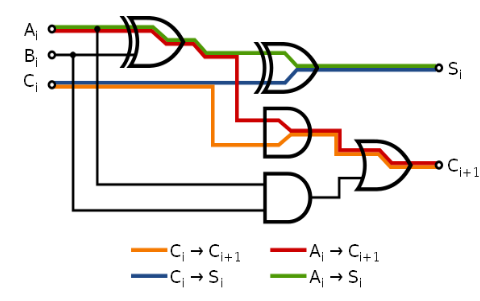
\includegraphics[scale=0.3]{./images/netlist_3.png}
      \end{center}
    \end{column}
  \end{columns}

\end{frame}



\begin{frame}{Circuits reconfigurables : FPGA}
  \begin{columns}[T]
    \begin{column}{0.5\textwidth}
      \begin{itemize}
        \item Coût élevé d'un circuit \textbf{ASIC} \textit{custom}...
        \item \textbf{FPGA} (1985) : circuit \textit{reconfigurable} à volonté.
        \begin{itemize}
          \item Approche \textit{Software-like} \footnote{voir TD \texttt{LUT2} où la notion de \textit{bitstream} sera expliquée.}
          \item Parallélisme équationnel booléen \textit{massif}.
        \end{itemize}
        \item Excellents pour :
        \begin{itemize}
          \item Prototypage, expérimentation.
          \item Faible volume de production.
          \item Fréquences de fonctionnement modérées.
          \item Existent aussi sous forme d'IP.
        \end{itemize}
        \item Fournisseurs :
        \begin{itemize}
          \item Xilinx (AMD), Altera (Intel)
          \item Lattice, Microchip (Microsemi)
          \item \textit{noeuds} technologiques avancés
          \item Equivalent de millions de portes logiques.
        \end{itemize}
      \end{itemize}
    \end{column}
    \begin{column}{0.5\textwidth}
      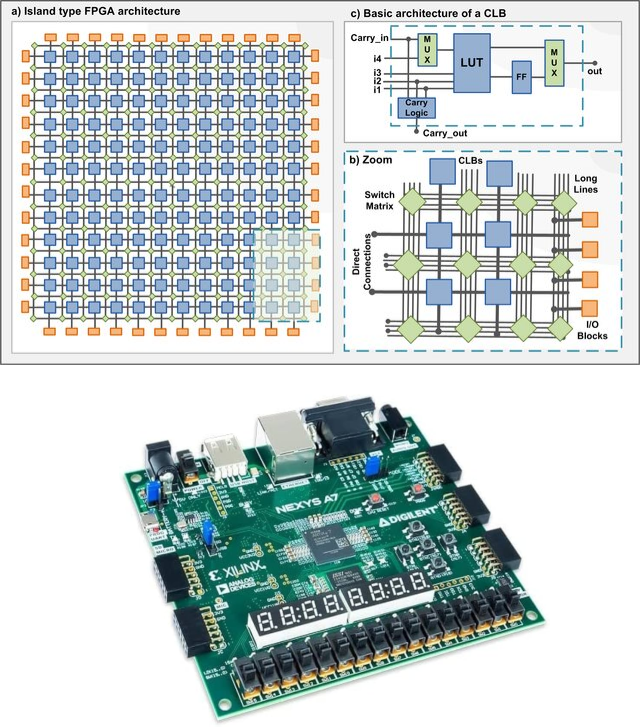
\includegraphics[scale=0.34]{./images/fpga_1.png}
    \end{column}
  \end{columns}
\end{frame}

\begin{frame}{FPGA : loin des circuits discrets !}
  \begin{center}
    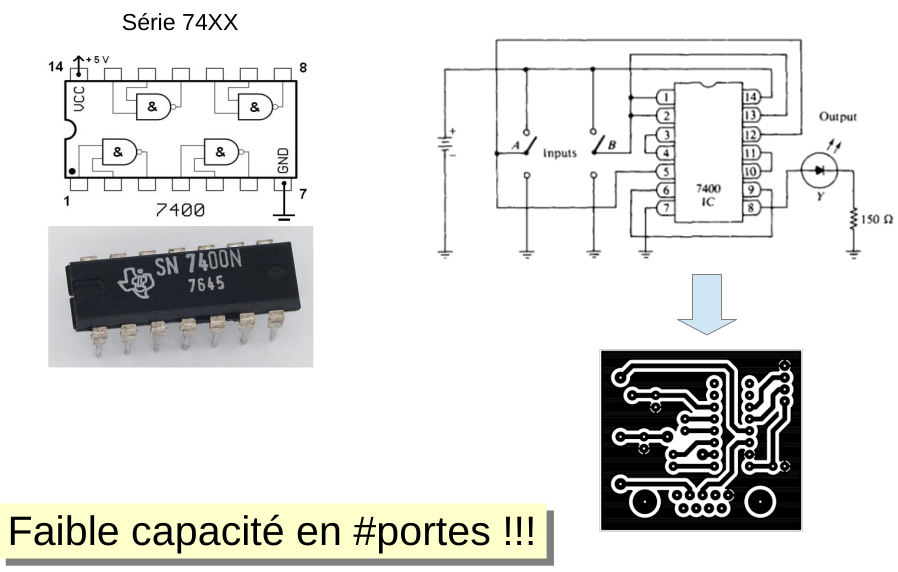
\includegraphics[scale=0.3]{./images/mapping.png}
  \end{center}
\end{frame}

%\section{Exemples de circuits combinatoires usuels}

% =========================================================
\begin{frame}{Additionneur à propagation de retenue (RCA) : $A+B$}

    \textbf{Principe :} chaîner $n$ additionneurs complets (FA)
    en propagant la retenue $C_i$ de proche en proche
    \textbf{du LSB vers le MSB}.

    \vspace{0.2cm}

    \begin{columns}
        \begin{column}{0.45\textwidth}
            \textbf{Additionneur complet (FA) :}
            \begin{align*}
                S_i &= A_i \oplus B_i \oplus C_i \\
                C_{i+1} &= A_i B_i + (A_i \oplus B_i)\, C_i
            \end{align*}

            \textbf{Table de vérité du FA :}
            \begin{center}
              \footnotesize
              \begin{tabular}{ccc|cc}
                \toprule
                $A_i$ & $B_i$ & $C_i$ & $S_i$ & $C_{i+1}$ \\
                \midrule
                0 & 0 & 0 & 0 & 0 \\
                0 & 0 & 1 & 1 & 0 \\
                0 & 1 & 0 & 1 & 0 \\
                0 & 1 & 1 & 0 & 1 \\
                1 & 0 & 0 & 1 & 0 \\
                1 & 0 & 1 & 0 & 1 \\
                1 & 1 & 0 & 0 & 1 \\
                1 & 1 & 1 & 1 & 1 \\
                \bottomrule
              \end{tabular}
            \end{center}
        \end{column}

        \begin{column}{0.55\textwidth}
          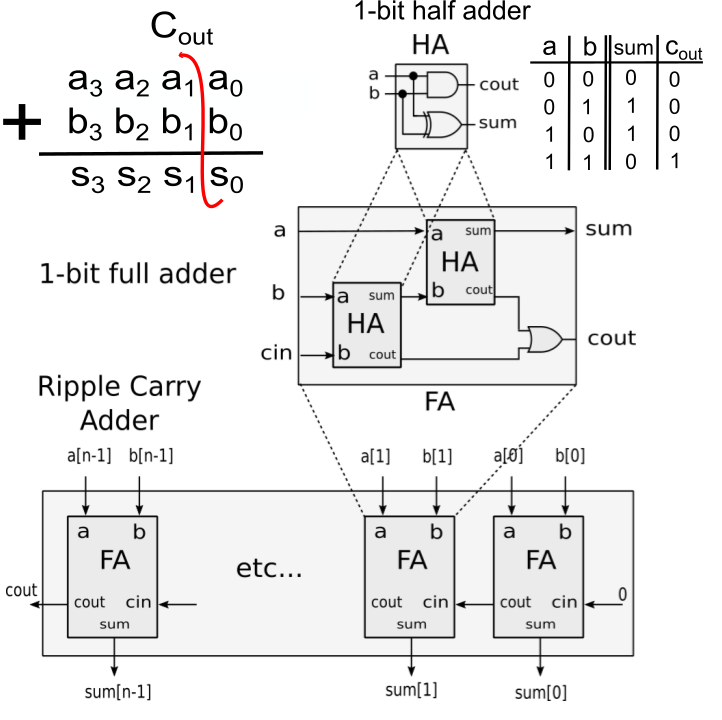
\includegraphics[scale=0.35]{./images/ripple_carry_adder.png}
        \end{column}
    \end{columns}

    %
    % \begin{block}{Point clé}
    %     \textbf{Temps critique} : $O(n)$ à cause de la propagation
    %     en cascade de la retenue (de droite à gauche). D'où les
    %     variantes plus rapides (CLA, carry-select, carry-skip).
    % \end{block}
\end{frame}

\begin{frame}{Soustracteur}
    \textbf{Principe :} réutiliser un additionneur \(n\) bits en agissant sur le second opérande via des portes \texttt{NOT} et injectant une retenue entrante.

    \vspace{0.3cm}

    \begin{columns}[T]
        \begin{column}{0.55\textwidth}
            \textbf{Idée clé :} soustraire \(B\) revient à ajouter son complément à deux :
            \[
                A - B = A + -B = A + \overline{B} + 1
            \]
        \end{column}
        \begin{column}{0.45\textwidth}
            \begin{center}
              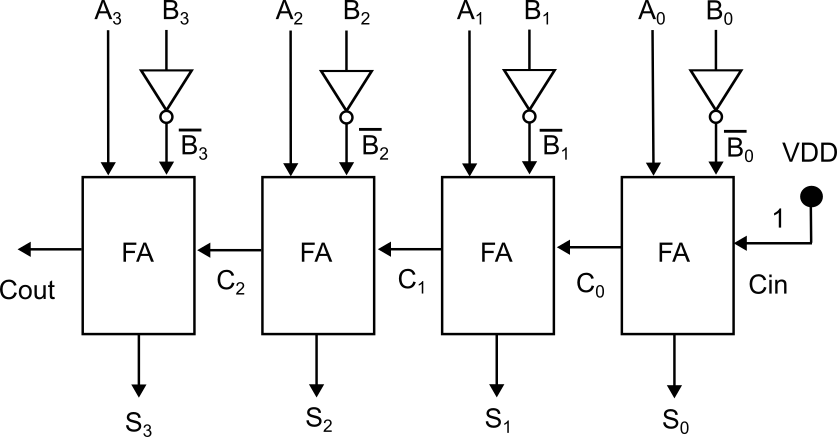
\includegraphics[scale=0.3]{./images/substractor.png}
            \end{center}
        \end{column}
    \end{columns}

    \vspace{0.2cm}
    \begin{block}{Point clé}
        Une seule porte \texttt{NOT} par bit + une retenue d'entrée à \texttt{1}: l'additionneur devient un \emph{soustracteur} sans modifier sa structure interne.
    \end{block}
\end{frame}

\begin{frame}{Additionneur-Soustracteur : un composant \textit{programmable}}
    \textbf{Principe :} réutiliser un additionneur \(n\) bits en agissant sur le second opérande via des portes \texttt{XOR} commandées par un signal \(\mathrm{sub}\) également utilisé en retenue \textit{entrante}.

    \vspace{0.3cm}

    \begin{columns}[T]
        \begin{column}{0.55\textwidth}
            \centering
            \begin{tabular}{cc|c}
              \toprule
              $B_i$ & SUB & $B_i'$ \\
              \midrule
              0 & 0 & 0 \\
              0 & 1 & 1 \\
              1 & 0 & 1 \\
              1 & 1 & 0 \\
              \bottomrule
            \end{tabular}
            \begin{itemize}
                \item \textbf{sub = 0} : \(B_i' = B_i \oplus 0 = B_i\), \(C_{in}=0\)
                \begin{itemize}
                  \item \textbf{addition} \(A+B\)
                \end{itemize}
                \item \textbf{sub = 1} : \(B_i' = B_i \oplus 1 = \overline{B_i}\), \(C_{in}=1\)
                \begin{itemize}
                  \item \textbf{soustraction} \(A-B\)
                \end{itemize}
            \end{itemize}
        \end{column}
        \begin{column}{0.45\textwidth}
            \begin{center}
              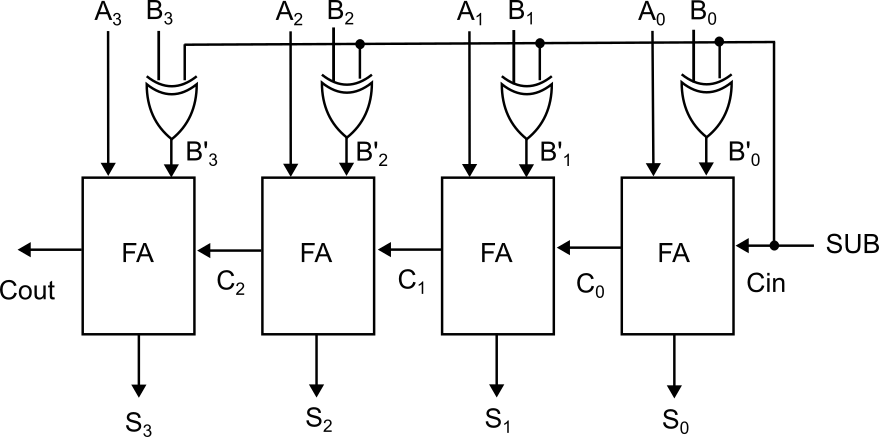
\includegraphics[scale=0.3]{./images/adder_substractor.png}
            \end{center}
        \end{column}
    \end{columns}

    \vspace{0.2cm}
    \begin{block}{Point clé}
        Une seule porte XOR par bit + une retenue d'entrée : l'additionneur devient un \emph{additionneur-soustracteur} sans modifier sa structure interne.
    \end{block}
\end{frame}
%==========================================================
\begin{frame}{Multiplieur (Mult)}

    \textbf{Principe :} suite
    d'additions décalées (algorithme « papier-crayon »).

    \vspace{0.2cm}

    \textbf{Formule booléenne (produit partiel) :}
    $PP_j = A \times b_j = A \cdot b_j \quad \text{(ET bit à bit)}$

    \textbf{Résultat :}
    $P = \sum_{j=0}^{n-1} \big( A \times b_j \big) \ll j$

    \begin{columns}
        \begin{column}{0.50\textwidth}
            \begin{center}
            \footnotesize

            \begin{tabular}{cc|c}
              \toprule
              $a_i$ & $b_j$ & $a_i \times_A b_i$ \\
              \midrule
              0 & 0 & 0 \\
              0 & 1 & 0 \\
              1 & 0 & 0 \\
              1 & 1 & 1 \\
              \bottomrule
            \end{tabular}

            \vspace{0.4cm}

            \begin{tabular}{r|cccc}
                & $a_3$ & $a_2$ & $a_1$ & $a_0$ \\
                $\times$ & $b_3$ & $b_2$ & $b_1$ & $b_0$ \\
                \midrule
                & $a_3 b_0$ & $a_2 b_0$ & $a_1 b_0$ & $a_0 b_0$ \\
                $a_3 b_1$ & $a_2 b_1$ & $a_1 b_1$ & $a_0 b_1$ & \\
                $a_2 b_2$ & $a_1 b_2$ & $a_0 b_2$ & &\\
                $a_1 b_3$ & $a_0 b_3$ & & &\\
                \bottomrule
                $p_4$ & $p_3$ & $p_2$ & $p_1$ & $p_0$ \\
            \end{tabular}
            \end{center}
        \end{column}

        \begin{column}{0.47\textwidth}
            %\footnotesize
            % \textbf{Architecture :}
            % \begin{itemize}
            %     \item $n$ portes ET (produits partiels)
            %     \item $n-1$ RCA en cascade
            %     \item Chaque RCA traite $n$ bits
            % \end{itemize}
            %
            % \vspace{0.2cm}
            % Complexité : $O(n^2)$ portes.
            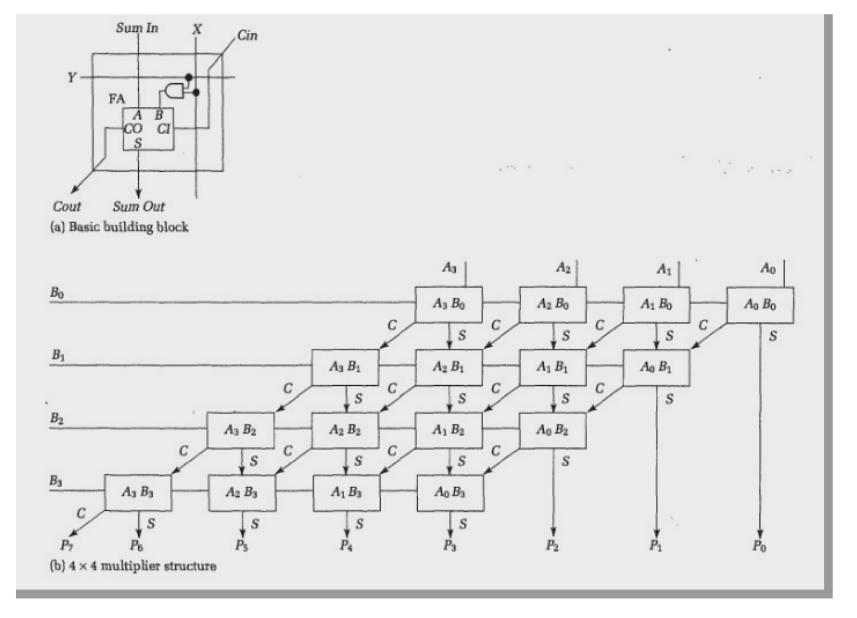
\includegraphics[scale=0.25]{./images/mult_topo.png}
        \end{column}
    \end{columns}

\end{frame}

% =========================================================
\begin{frame}{Multiplexeur 2 vers 1 (MUX21)}

    \textbf{Rôle :} sélectionner une entrée parmi deux selon un signal de commande.

    \vspace{0.1cm}

    \begin{columns}
        \begin{column}{0.5\textwidth}
          \textbf{Table de vérité :}
          \begin{tabular}{ccc|c}
                \toprule
                $A$ & $B$ & $Sel$ & $F$ \\
                \midrule
                $0$ & $0$ & $0$ & $0$ \\
                $0$ & $0$ & $1$ & $0$ \\
                $0$ & $1$ & $0$ & $0$ \\
                $0$ & $1$ & $1$ & $1$ \\
                $1$ & $0$ & $0$ & $1$ \\
                $1$ & $0$ & $1$ & $0$ \\
                $1$ & $1$ & $0$ & $1$ \\
                $1$ & $1$ & $1$ & $1$ \\
                \bottomrule
            \end{tabular}

            \vspace{0.3cm}
            \textbf{Formule booléenne :}
            $F = \overline{Sel} \times A + Sel \times B$

            \vspace{0.1cm}
        \end{column}

        \begin{column}{0.48\textwidth}
            \begin{center}
                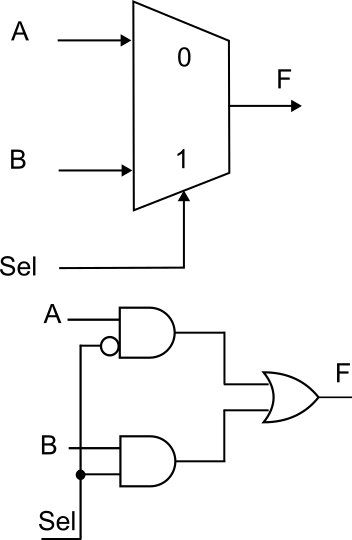
\includegraphics[scale=0.35]{./images/mux21.png}
            \end{center}
        \end{column}
    \end{columns}

    \vspace{0.1cm}

    \begin{block}{Application}
        Brique de base des MUX $2^n$→1, des barrel shifters et
        de la logique reconfigurable (FPGA).
    \end{block}

\end{frame}

% =========================================================
\begin{frame}{Shifter à position fixe (décalage par câblage)}

    \textbf{Idée clé :} décaler une donnée d'un nombre \textbf{constant}
    de positions ne nécessite \textbf{aucune porte logique}--
    un simple \textbf{recâblage} suffit.

    \vspace{0.3cm}

    \begin{columns}
        \begin{column}{0.52\textwidth}
            \textbf{Formule booléenne (décalage logique à gauche de $k$) :}
            $$S_i = \begin{cases} A_{i-k} & \text{si } i \geq k \\[2pt] 0 & \text{si } i < k \end{cases}$$

            \vspace{0.3cm}

            \textbf{Décalage logique à droite de $k$ :}
            $$S_i = \begin{cases} A_{i+k} & \text{si } i+k < n \\[2pt] 0 & \text{sinon} \end{cases}$$

            \vspace{0.3cm}

            \footnotesize Chaque sortie $S_i$ est reliée \emph{directement}
            à une entrée $A_j$ ou à la masse (0).
        \end{column}

        \begin{column}{0.46\textwidth}
            \textbf{Exemple : $A$ sur 4 bits, SLL de 1 ($k=1$)}

            \vspace{0.3cm}

            \begin{center}
            \footnotesize
            \begin{tabular}{l|cccc}
                \toprule
                Entrée A & $A_3$ & $A_2$ & $A_1$ & $A_0$\\
                \midrule
                Sortie S & $A_2$ & $A_1$ & $A_0$ & $0$ \\
                \bottomrule
            \end{tabular}
            \end{center}

            \vspace{0.3cm}

            \footnotesize Aucun composant actif : juste des fils !
        \end{column}
    \end{columns}

\end{frame}


\begin{frame}{Comparateur d'égalité de 2 mots binaires}
    \textbf{Objectif :} produire un signal \(E=1\) si et seulement si
    \(A = B\), avec \(A = A_{n-1}\dots A_0\) et \(B = B_{n-1}\dots B_0\).

    \vspace{0.2cm}

    \begin{columns}[T]
        \begin{column}{0.52\textwidth}
            \textbf{Principe :} comparer \emph{bit à bit} puis combiner.
            \[
                e_i = \overline{A_i \oplus B_i}
                \qquad (\text{XNOR})
            \]
            \[
                E = \prod_{i=0}^{n-1} \overline{A_i \oplus B_i}
            \]
            \begin{itemize}
                \item \(A_i = B_i \Rightarrow e_i = 1\)
                \item \(A_i \neq B_i \Rightarrow e_i = 0\) (et \(E=0\))
            \end{itemize}
        \end{column}
        \begin{column}{0.48\textwidth}
            \begin{center}
            \begin{circuitikz}[scale=0.5, transform shape]
                % XNOR gates (représentées par XOR + NON)
                \foreach \i/\y in {0/0, 1/-1.6, 2/-3.2, 3/-4.8} {
                    \node[xor port] (xor\i) at (0,\y) {};
                    \node[left] at (xor\i.in 1) {\(A_{\i}\)};
                    \node[left] at (xor\i.in 2) {\(B_{\i}\)};
                    \node[not port, scale=0.5] (not\i) at (2.2,\y) {};
                    \draw (xor\i.out) -- (not\i.in);
                    \node[right] at (not\i.out) {\scriptsize \(e_{\i}\)};
                }
                % AND tree
                \node[and port] (and0) at (4.8,-0.8) {};
                \node[and port] (and1) at (4.8,-4.0) {};
                \draw (not0.out) -- ++(0.3,0) |- (and0.in 1);
                \draw (not1.out) -- ++(0.3,0) |- (and0.in 2);
                \draw (not2.out) -- ++(0.3,0) |- (and1.in 1);
                \draw (not3.out) -- ++(0.3,0) |- (and1.in 2);

                \node[and port] (andF) at (7.6,-2.4) {};
                \draw (and0.out) -- ++(0.3,0) |- (andF.in 1);
                \draw (and1.out) -- ++(0.3,0) |- (andF.in 2);

                \draw[->] (andF.out) -- ++(0.8,0) node[right] {\(E\)};
            \end{circuitikz}
            \end{center}
        \end{column}
    \end{columns}

    \vspace{0.1cm}
    \begin{block}{Point clé}
        \(n\) portes \textbf{XNOR} en parallèle (une par bit) + un \textbf{ET} global
        (arbre d'AND) pour agréger les égalités partielles.
    \end{block}
\end{frame}



%============================================================
\begin{frame}{Décodeur $n \to 2^n$}
    \textbf{Principe :} Un décodeur $n \to 2^n$ active une seule sortie parmi $2^n$
    en fonction du code binaire présent en entrée.

    \vspace{0.1cm}

    \textbf{Entrées :} $A_1, A_0$ \hfill \textbf{Sorties :} $S_0, S_1, S_2, S_3$

    \vspace{0.1cm}

    \begin{columns}
        \begin{column}{0.5\textwidth}
            \textbf{Équations booléennes :}
            \begin{align*}
                S_0 &= \overline{A_1}\,\overline{A_0} \\
                S_1 &= \overline{A_1}\,A_0 \\
                S_2 &= A_1\,\overline{A_0} \\
                S_3 &= A_1\,A_0
            \end{align*}

            \vspace{0.1cm}
            Forme compacte :
            $$S_i = \prod_{k=0}^{n-1} \left( A_k \oplus \overline{b_{i,k}} \right)$$

            \vspace{0.05cm}
            \footnotesize où $b_{i,k}$ est le $k$-ième bit de la
            représentation binaire de l'indice $i$.
        \end{column}

        \begin{column}{0.48\textwidth}
            \textbf{Tableau de principe :}
            \begin{center}
                \begin{tabular}{cc|cccc}
                    \toprule
                    $A_1$ & $A_0$ & $S_0$ & $S_1$ & $S_2$ & $S_3$ \\
                    \midrule
                    0 & 0 & \textbf{1} & 0 & 0 & 0 \\
                    0 & 1 & 0 & \textbf{1} & 0 & 0 \\
                    1 & 0 & 0 & 0 & \textbf{1} & 0 \\
                    1 & 1 & 0 & 0 & 0 & \textbf{1} \\
                    \bottomrule
                \end{tabular}
            \end{center}

            \vspace{0.3cm}
            \footnotesize\textbf{Exemple :} pour $i=2$, on a
            $(b_{2,1}\,b_{2,0})_2 = (10)_2$, donc
            $b_{2,1}=1$ et $b_{2,0}=0$.
        \end{column}
    \end{columns}
\end{frame}


\begin{frame}{Décodeur BCD vers afficheur 7 segments}
  \begin{center}
      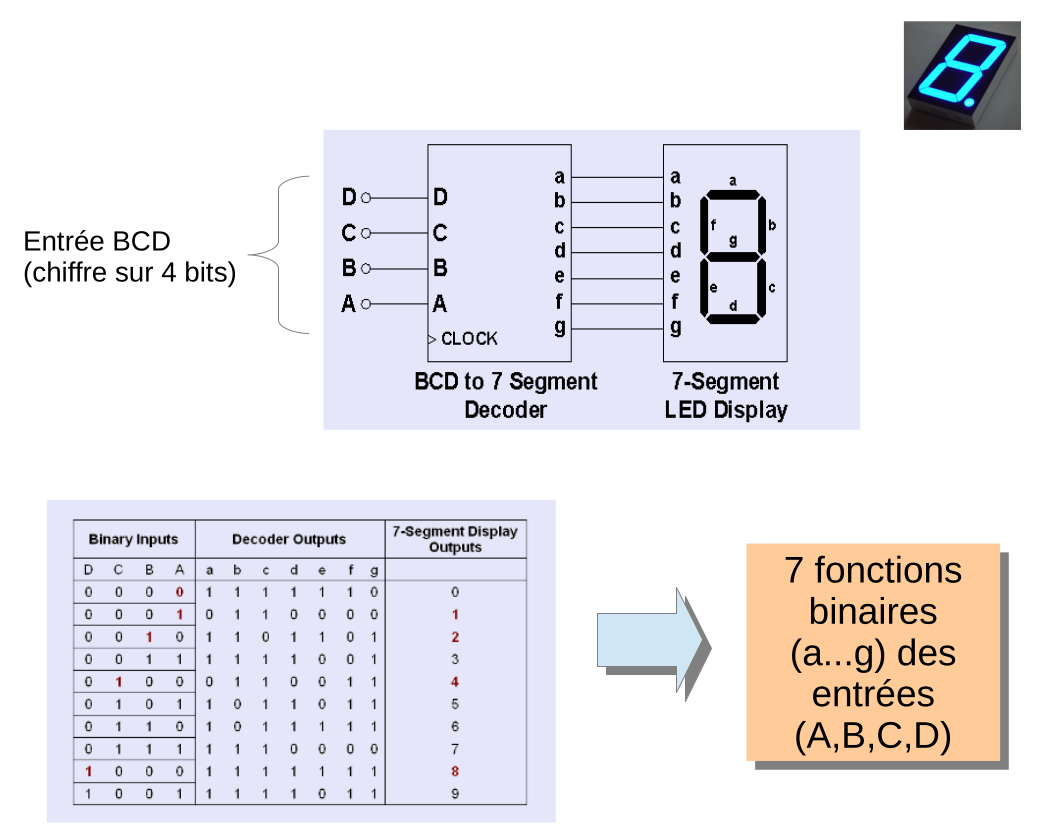
\includegraphics[scale=0.25]{./images/decoder_7seg.png}
  \end{center}
\end{frame}

% %========================================================================================
%\section{Logique Séquentielle}
% % %========================================================================================
%
\begin{frame}{Combinatoire : maîtrise difficile des signaux}
    \begin{block}{Rappel : La logique combinatoire}
        Les sorties ne dépendent que des entrées présentes. Mais en pratique... le temps existe !
    \end{block}

    %\vspace{0.3em}
    \begin{columns}
        \column{0.60\textwidth}
        \textbf{Problématiques physiques :}
        \begin{itemize}
            \item \textbf{Délais de propagation (\(\tau_{pd}\)) :} Les portes mettent du temps à calculer (durée non-déterministe).
            \item \textbf{Aléas (hazards) :} Apparition de transitoires parasites lors de changements simultanés.
        \end{itemize}
        \vspace{0.1em}
        \textbf{Conséquences en cascade :}
        \begin{itemize}
          \item Impossible de prédire exactement \textit{à partir de} \textbf{quand} un signal est stable.
          \item \textbf{Composer} de grands blocs combinatoires mène à un chaos temporel ingérable.
        \end{itemize}
        \begin{alertblock}{Constat}
          La complexité des systèmes explose et la fiabilité s'effondre.
        \end{alertblock}

        \column{0.35\textwidth}
        %\begin{center}
          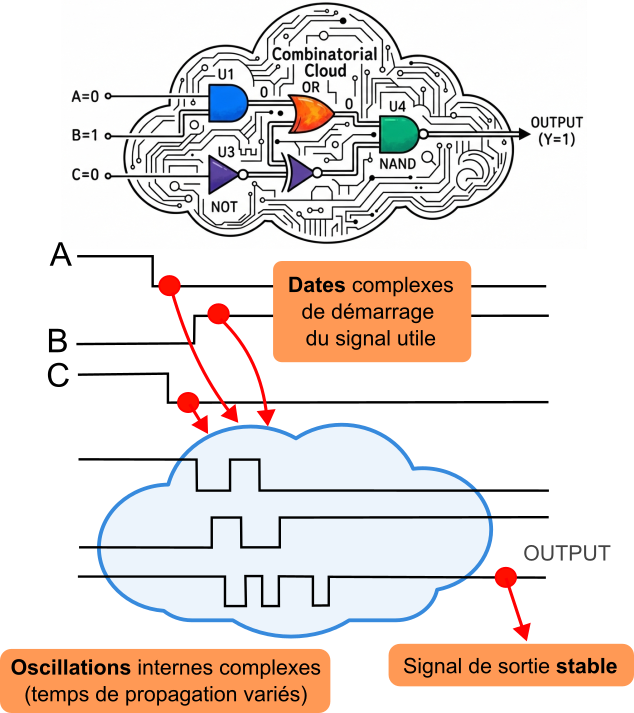
\includegraphics[scale=0.31]{./images/bascule_d_v0.png}
        %\end{center}
    \end{columns}

\end{frame}
%
% \begin{frame}{Combinatoire : maîtrise difficile des signaux}
%   \begin{center}
%     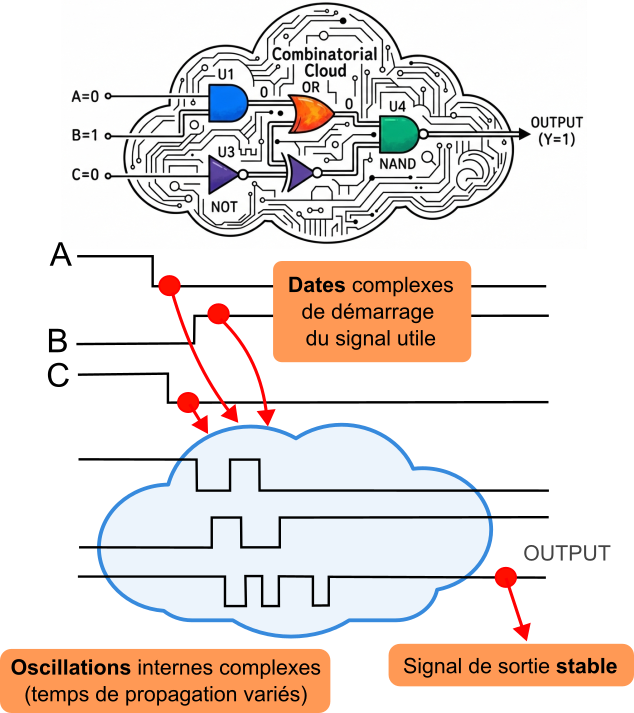
\includegraphics[scale=0.4]{./images/bascule_d_v0.png}
%   \end{center}
% \end{frame}

\begin{frame}{Le système synchrone mono-cadencé : Maîtriser le temps}
    \begin{block}{L'idée directrice}
        Plutôt que de subir les délais continus, on segmente le temps à l'aide d'un \textbf{métronome commun, unique}  : \textbf{l'horloge}. Elle est suffisamment lente pour que tous les signaux se stabilisent avant leur échantillonnage.
    \end{block}

    \vspace{0.3em}
    \begin{itemize}
        \item \textbf{Le quantum de temps :} Le cycle d'horloge (\(T\)) devient l'unique unité de référence.
        \item \textbf{Séparation des rôles :}
        \begin{itemize}
            \item Le \textit{combinatoire} calcule la nouvelle valeur (pendant que le signal se stabilise).
            \item La \fbox{\textit{bascule D}} mémorise cette valeur au moment précis du front d'horloge (montant pour nous).
        \end{itemize}
        \item \textbf{Bénéfice majeur :} On s'affranchit des variations technologiques et des délais intermédiaires ; on ne raisonne plus en nanosecondes, mais en \textbf{coups d'horloge}.
    \end{itemize}

    \vspace{0.5em}
    \begin{exampleblock}{Conclusion}
        La \fbox{bascule D} est la brique de base qui permet de synchroniser le monde et de passer du « temps continu incertain » au « temps discret maîtrisé ».
    \end{exampleblock}
\end{frame}


\begin{frame}{Bascule D : symbole, table de vérité et chronogramme}
  \begin{center}
    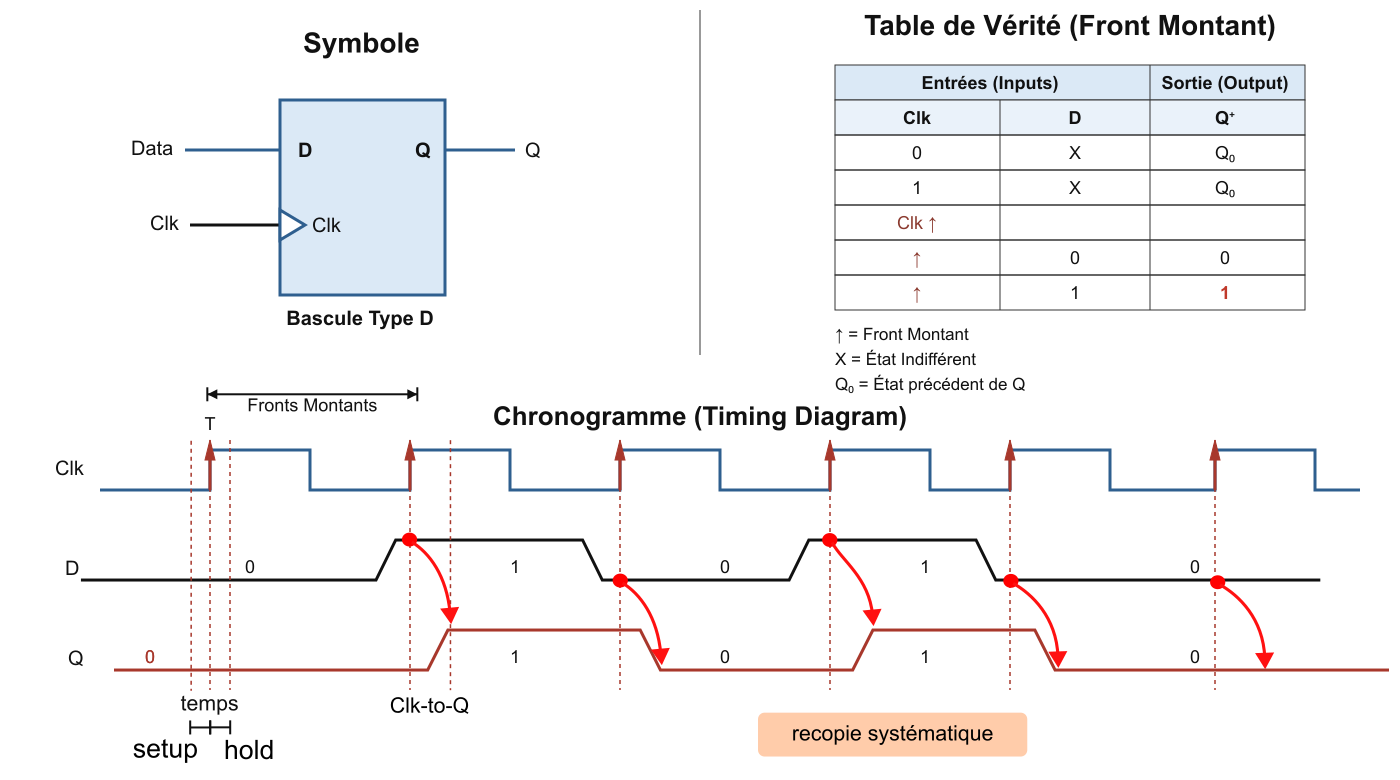
\includegraphics[scale=0.35]{./images/bascule_d.png}
  \end{center}
\end{frame}


\begin{frame}{La bascule D : un décalage d’un cycle d’horloge}
  %\framesubtitle{Du comportement microscopique au point de vue macroscopique}

  \begin{block}{Ce qu’il faut retenir}
    Une bascule D recopie l’entrée \(D\) sur la sortie \(Q\) \textbf{au rythme de l’horloge}.
    \[
      Q_{n+1} = D_n
    \]
    Autrement dit : \alert{\(Q\) est la version de \(D\), retardée d’un cycle }.
  \end{block}

  \vspace{0.1cm}

  \begin{columns}[T]
    \begin{column}{0.48\textwidth}
      \textbf{Vue microscopique (complexe)}
      \begin{itemize}
        \item chronogramme détaillé.
        \item temps de \emph{setup} et de \emph{hold}
        \item recopie exacte après le délai \(t_{\text{Clk}\to Q}\)
        \item phénomènes transitoires
      \end{itemize}

    \end{column}

    \begin{column}{0.48\textwidth}
      \textbf{Vue macroscopique (simple)}
      \begin{itemize}
        \item on oublie les détails temporels fins
        \item on attend que tous les signaux soient stables : $T_{clock} >> \text{max}(\{T_{crit}(f)\},\forall f \in \mathbb{O})$
        \item on ne garde que : \alert{un coup d’horloge = un pas de retard}
      \end{itemize}
    \end{column}
  \end{columns}

  \begin{alertblock}{On bascule dans l’Informatique !}
    La bascule D transforme un signal continu en \textbf{suite numérique}.
  \end{alertblock}
\end{frame}

\begin{frame}{Bascule D : précautions d'utilisation}
  \begin{columns}
    \begin{column}{0.5\textwidth}
      \begin{enumerate}
        \item Le signal \texttt{D} doit être stable \underline{avant} et \underline{après} le front montant.
        \begin{itemize}
          \item temps de \texttt{setup}
          \item temps de \texttt{hold}
        \end{itemize}
        \item Sinon : risque de \textbf{métastabilité}
        \begin{itemize}
          \item tension intermédiaire imprévisible
          \item ...avant stabilisation aléatoire (O ou 1)
          \item ...au bout d'un délai variable
        \end{itemize}
      \end{enumerate}
      \begin{center}
        \includegraphics[scale=0.15]{./images/hill.jpg}
      \end{center}
    \end{column}
    \begin{column}{0.5\textwidth}
      \begin{enumerate}[3]
        \item Le \textbf{passé} du signal \texttt{D} se trouve sur la sortie \texttt{Q}
      \end{enumerate}
      \begin{center}
        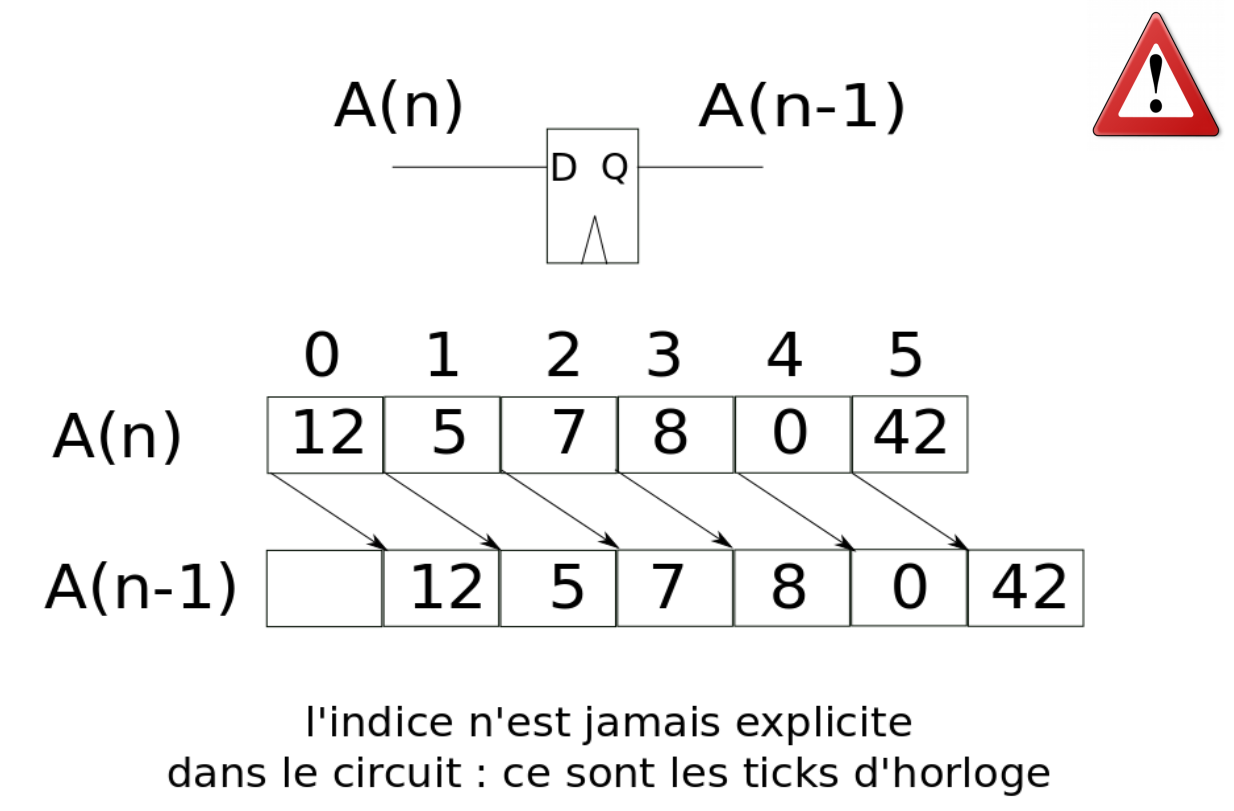
\includegraphics[scale=0.18]{./images/bascule_d_indices.png}
      \end{center}
    \end{column}
  \end{columns}
\end{frame}

\begin{frame}{Bascule D : constitution interne}

  \begin{alertblock}{Attention : \textit{"Ne pas reproduire à la maison"}}
    \begin{itemize}
      \item La règle de \texttt{conception synchrone} \fbox{interdit} les \textbf{cycles combinatoires}.
      \begin{itemize}
        \item Il est difficile \texttt{de savoir} si une boucle stabilise ou pas (ici oui).
        \item Veiller à ne pas introduire de telles boucles de manière subtile.
        \item Ne conservez que la bascule D. Oubliez les autres.
      \end{itemize}
    \end{itemize}
  \end{alertblock}

  \begin{center}
      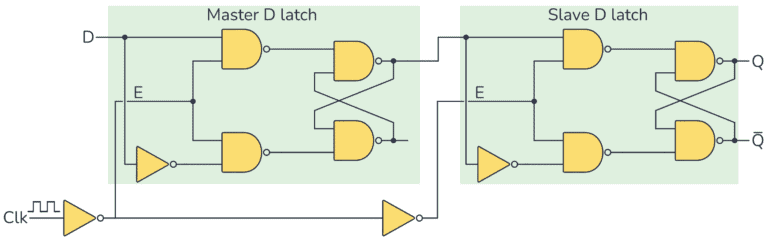
\includegraphics[scale=0.3]{./images/dff.png}
  \end{center}

  \begin{block}{Info}
    Plusieurs structures internes de bascule D. En CMOS notamment : portes de transmission.
  \end{block}
\end{frame}


\begin{frame}{Bascule D : mémorisation par \textit{recirculation} des données}
  \begin{alertblock}{Objectif}
    Comment mémoriser une \underline{même} donnée \textbf{pendant plusieurs cycles} ?
  \end{alertblock}

  \begin{columns}
    \begin{column}{0.5\textwidth}
      \begin{itemize}
        \item \textbf{Rappel} :
        \begin{itemize}
          \item la bascule D mémorise son état durant \underline{une} période d'horloge
          \item un nouveau front $\rightarrow$ échantillonnne une \underline{nouvelle} donnée sur \texttt{D}.
        \end{itemize}
        \item \textbf{Solution : }\fbox{Recirculation} à l'aide d'un \texttt{multiplexeur} \footnote{rappel : le multiplexeur est combinatoire}.
        \begin{enumerate}
          \item Un signal de contrôle (ici \texttt{load}) accompagne la donnée entrante \texttt{A}.
          \item La bascule \texttt{D} ré-échantillonne la donnée capturée, présente sur \texttt{F}, à chaque cycle.
        \end{enumerate}
      \end{itemize}
      % \begin{block}{Note}
      %   Il existe aussi des langages \textit{informatiques} qui utilisent le \textbf{modèle synchrone} : systèmes critiques, avionique,...
      % \end{block}
    \end{column}
    \begin{column}{0.5\textwidth}
      \begin{center}
        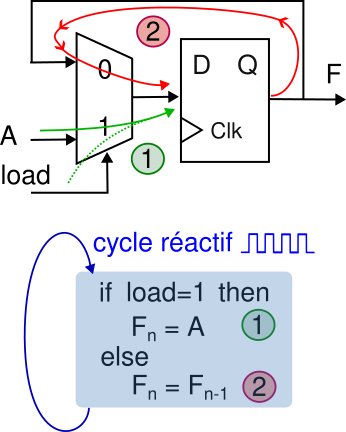
\includegraphics[scale=0.45]{./images/recirculation.png}
      \end{center}
    \end{column}
  \end{columns}
\end{frame}

\begin{frame}{Exemple : analyseur de sourires}
  \begin{columns}
    \begin{column}{0.5\textwidth}
      \begin{center}
        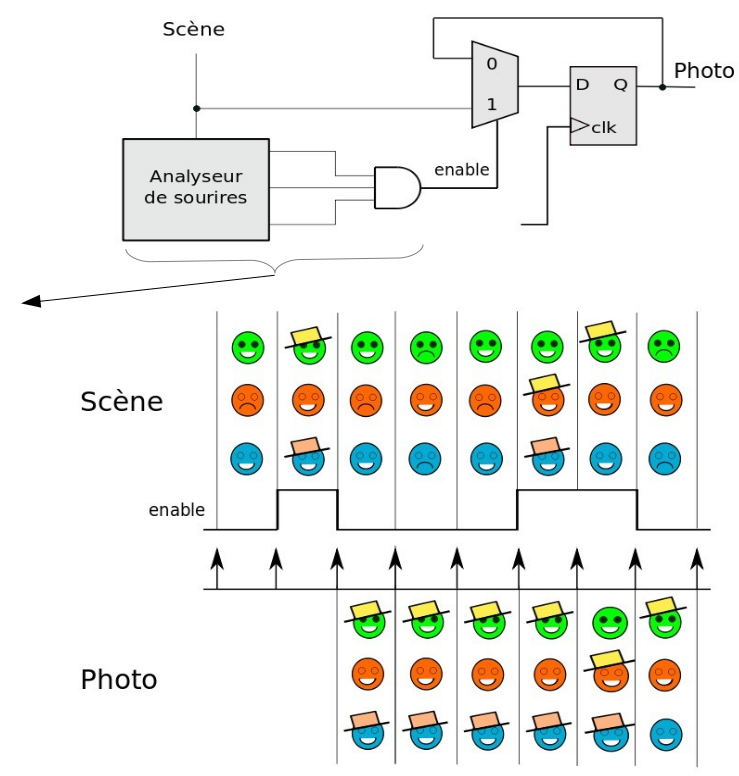
\includegraphics[scale=0.26]{./images/analyseur_sourires.png}
      \end{center}
    \end{column}
    \begin{column}{0.5\textwidth}
      $\leftarrow$ On suppose que l'analyseur est purement combinatoire....\\
      \vspace{0.5cm}
      \textbf{Apparition d'un schéma générique} :
      \begin{alertblock}{On retient :}
        \begin{itemize}
          \item Calculs "verticaux" : combinatoire.
          \item Calculs "horizontaux" : séquentiel.
        \end{itemize}
      \end{alertblock}
      \begin{itemize}
        \item La bascule D permet de passer d'un instant logique à un autre.
        \item La bascule D "coupe" des calculs combinatoires.
      \end{itemize}
    \end{column}
  \end{columns}
\end{frame}

\begin{frame}{Systèmes séquentiels : schéma générique}

\begin{columns}[T]
  % ---------- Colonne gauche : le circuit ----------
  \begin{column}{0.45\textwidth}
    \centering

    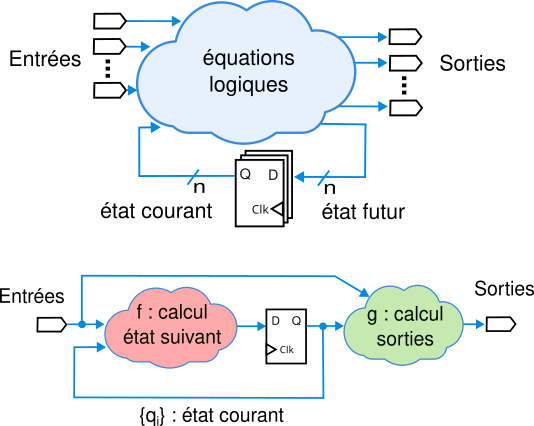
\includegraphics[scale=0.50]{./images/sys_0.png}

    \vspace{0.3cm}
    {\small Horloge implicite : le temps est discret, $t\in\mathbb{N}$.}
  \end{column}

  % ---------- Colonne droite : équations ----------
  \begin{column}{0.55\textwidth}
    \textbf{Bascule D :} $q(t+1) = d(t)$

    \medskip
    \textbf{Tout le circuit se ramène à :}
    \[
      \begin{cases}
        q_i(t+1) = d_i(t) = f_i\big(e(t),\,q(t)\big) & \text{(état suivant)}\\[2pt]
        s_j(t)   = g_j\big(e(t),\,q_j(t)\big) & \text{(sorties)}
      \end{cases}
    \]
    où $f_i,g_j$ sont des équations booléennes.

  \end{column}
\end{columns}

\end{frame}

%======================================================================
\begin{frame}{Systèmes séquentiels : schéma générique}
  \begin{columns}[T]
    % ---------- Colonne gauche : le circuit ----------
    \begin{column}{0.45\textwidth}
      \centering

      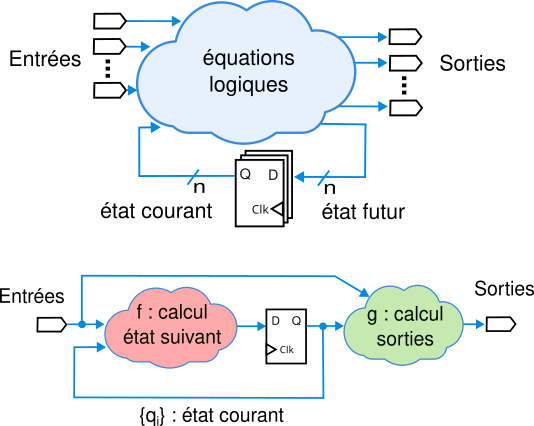
\includegraphics[scale=0.50]{./images/sys_0.png}

      \vspace{0.3cm}
      {\small Horloge implicite : le temps est discret, $t\in\mathbb{N}$.}
    \end{column}

    % ---------- Colonne droite : équations ----------

      \begin{column}{0.45\textwidth}
              \begin{block}{Analogie avec le monde continu}
                  \textbf{Monde continu (Physique/Syst. Dyn) :}
                  \[ \frac{d\mathbf{Q}}{dt} = \mathbf{f}(\mathbf{Q}, \mathbf{E}, t) \]
                  \vspace{0.2cm}
                  \textbf{Monde numérique (Discret) :}
                  \[ \mathbf{Q}_{t+1} = \mathcal{F}(\mathbf{Q}_t, \mathbf{E}_t) \]
                  \vspace{0.1cm}
                  \footnotesize L'horloge dicte le pas de temps : $dt \equiv T_{clk}$.
              \end{block}

              \begin{alertblock}{Le caractère \og exécutable \fg{}}
                  Contrairement aux équations différentielles sur le papier, le silicium \textbf{résout et exécute} ces équations en temps réel, front après front.
              \end{alertblock}
          \end{column}

  \end{columns}
\end{frame}
%======================================================================
\begin{frame}{Systèmes séquentiels : schéma générique et déclinaisons}
  \centering
  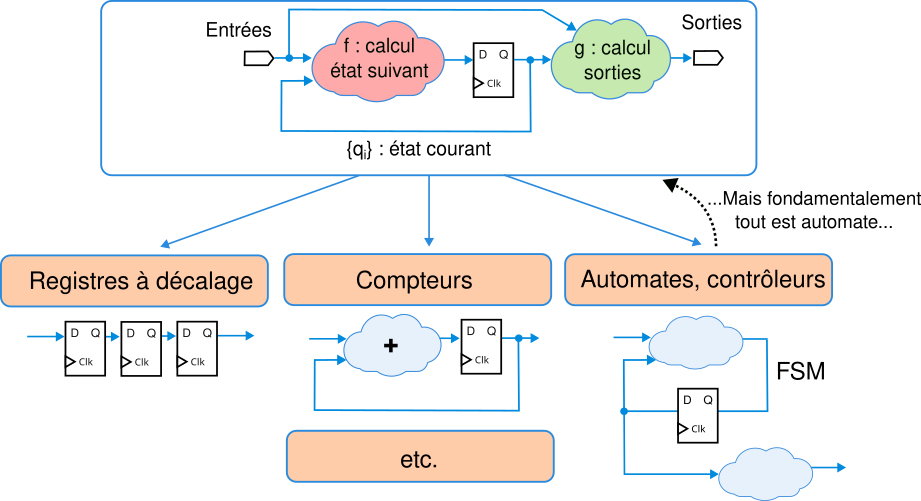
\includegraphics[scale=0.50]{./images/seq_3.png}

  \begin{center}
        \textbf{Conséquence :} Tout système dynamique discret, automate ou algorithme \\peut être \alert{matérialisé et simulé} par un réseau de bascules. \\
        \normalsize $\rightarrow$ \textit{Le circuit numérique possède un pouvoir de modélisation universel.}
    \end{center}
\end{frame}


\begin{frame}{Bascule D : Reset et Set \textit{asynchrones}}
\begin{columns}
  \begin{column}{0.45\textwidth}
    \begin{block}{Cas du \texttt{Reset} : mise à 0}
      \begin{itemize}
        \item Le \texttt{reset} est \textbf{prioritaire} sur l'horloge.
        \item Lorsqu'il est activé $\rightarrow Q=0$
      \end{itemize}
    \end{block}
    \begin{exampleblock}{Cas du \texttt{Set} : mise à 1}
      \begin{itemize}
        \item Le \texttt{set} est \textbf{prioritaire} sur l'horloge.
        \item Lorsqu'il est activé $\rightarrow Q=1$
      \end{itemize}
    \end{exampleblock}
    En cas d'ordres contradictoires $\rightarrow$ voire doc constructeur.

  \end{column}
  \begin{column}{0.45\textwidth}
    \centering
    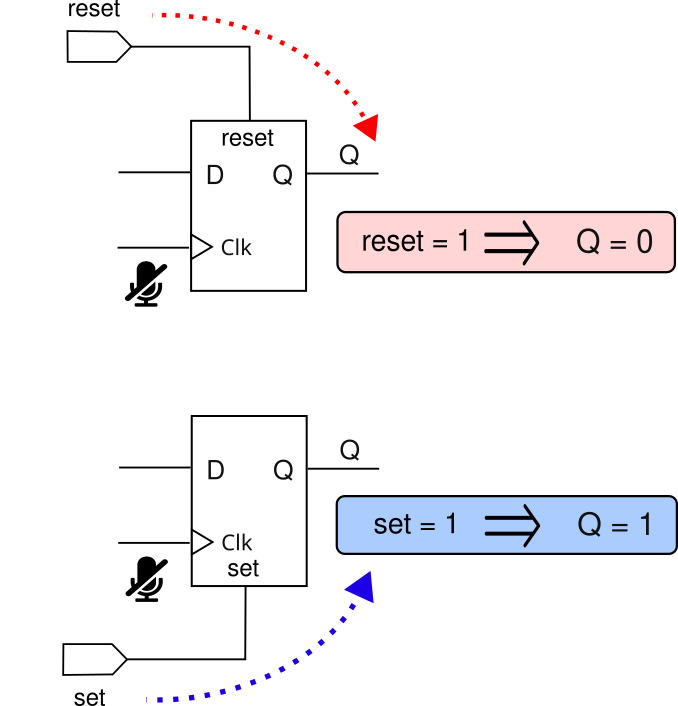
\includegraphics[scale=0.4]{./images/reset_0.png}
  \end{column}
\end{columns}
\end{frame}

\begin{frame}{Bascule D : Reset et Set \textit{asynchrones}}
\begin{columns}
  \begin{column}{0.40\textwidth}
    \centering
    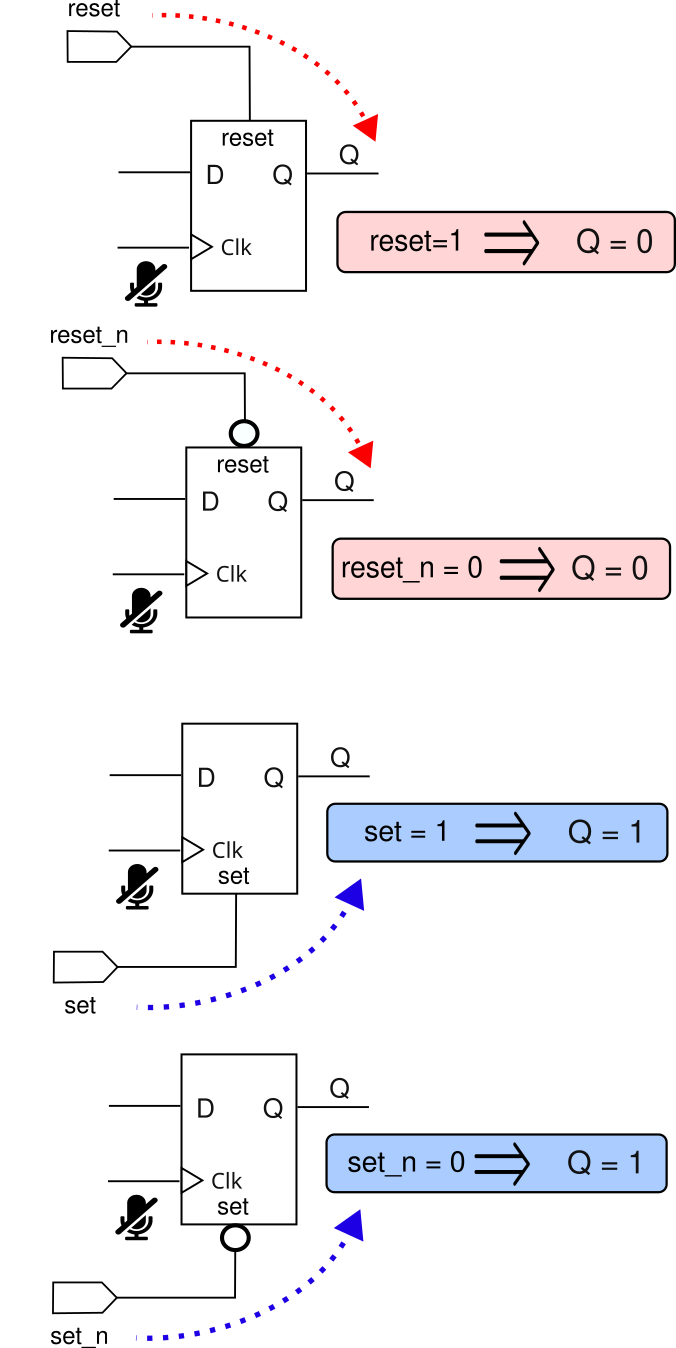
\includegraphics[scale=0.21]{./images/reset_1.png}
  \end{column}
  \begin{column}{0.55\textwidth}
    \begin{block}{Polarité d'activation}
      \begin{itemize}
        \item  Les deux signaux \texttt{reset} et \texttt{set} ont eux-mêmes une valeur où ils sont
        actifs.
        \item Cette valeur est précisée dans le schéma de la bascule :
        \begin{itemize}
          \item Cerle ° indique la \fbox{polarité \texttt{0} active}.
          \item L'\underline{absence de cercle} ° indique la \fbox{polarité \texttt{1} active}.
        \end{itemize}
        \item Cette valeur \textit{peut} être précisée dans le \textit{nommage} du signal :
        \begin{itemize}
          \item \texttt{reset\_n} indique une polarité \texttt{0} active.
          \item \texttt{reset} indique une polarité \texttt{1} active.
        \end{itemize}
      \end{itemize}
    \end{block}
    \begin{itemize}
      \item Les noms des signaux dépendent des \textit{conventions de nommage} propres aux entreprises.
      \item \textbf{Attention : } bien connecter \textbf{tous} les \texttt{reset} et \texttt{set}.
    \end{itemize}
  \end{column}
\end{columns}
\end{frame}

%\section{Automates ou \textit{Machines d'états Finis} (FSM)}

\begin{frame}{Du circuit au diagramme états-transitions}
  \begin{columns}
    \begin{column}{0.45\textwidth}
      \begin{itemize}
        \item \textbf{Rappel} : les valeurs des sorties $Q$ représentent l'état du système à un instant logique donné.
        \item Le nombre d'états possibles est donc \textbf{fini}.
        \item Il est plus intuitif de les représenter \textit{autrement} :
        \begin{itemize}
          \item \fbox{Diagramme états transitions}
        \end{itemize}
      \end{itemize}
    \end{column}
    \begin{column}{0.55\textwidth}
      \centering
      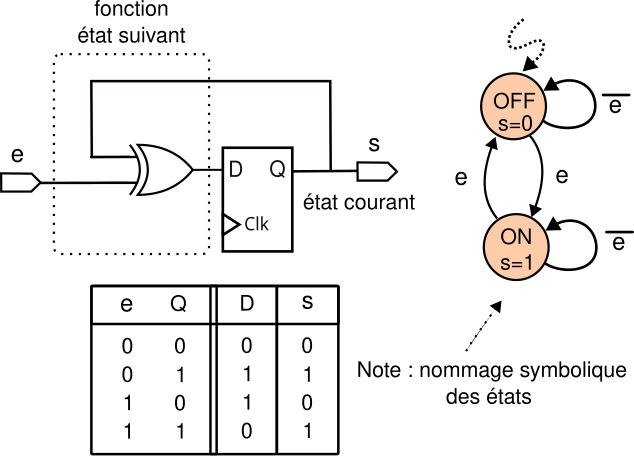
\includegraphics[scale=0.5]{./images/diag_0.png}
    \end{column}
  \end{columns}
\end{frame}


\begin{frame}{Diagramme états-transitions}
  \begin{columns}
    \begin{column}{0.5\textwidth}
      \begin{block}{Définition}
        Un diagramme états-transitions est un \textbf{graphe orienté valué}
        $G = (Q, A)$ où :
        \begin{itemize}
          \item $Q$ : ensemble \textbf{fini} de sommets (les \textit{états}).
          \item $E = \{e_1, \dots, e_n\}$ : signaux d'entrée binaires ;
          $\;\Sigma = \{0,1\}^n$ : espace des combinaisons d'entrée.
          \item $S = \{s_1, \dots, s_m\}$ : signaux de sortie binaires ;
          $\;\Lambda = \{0,1\}^m$ : espace des combinaisons de sortie.
          \item $\mathcal{C} \subseteq \mathcal{P}(\Sigma)$ : ensemble
          de \textit{conditions} (prédicats booléens sur les entrées).
          \item $A \subseteq Q \times \mathcal{C} \times \Lambda \times Q$ :
          ensemble des \textit{arcs orientés}.
        \end{itemize}
      \end{block}
    \end{column}
    \begin{column}{0.5\textwidth}
      \begin{center}
        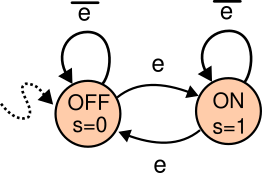
\includegraphics[scale=0.4]{./images/diag_1.png}
      \end{center}
      \begin{center}
      \small
      \textbf{Sémantique d'un arc :} \quad
      $q_i \xrightarrow{\ c\,/\,\lambda\ } q_j
      \;\iff\;
      (q_i,\; c,\; \lambda,\; q_j) \in A$
      \quad avec $c \in \mathcal{C}$
      \end{center}

      \vspace{0.15cm}
      {\small
      \begin{itemize}
        \item $c \in \mathcal{C}$ est un \textbf{prédicat} sur $\Sigma$
          (ex : $e_1 \land \lnot e_2$), permettant \textit{don't-cares}
          et regroupement de combinaisons.
        \item \textbf{Moore} : $\lambda$ dépend uniquement de $q_i$
          (sortie annotée sur le sommet).
        \item \textbf{Mealy} : $\lambda$ dépend de $q_i$ et de la
          combinaison d'entrée effective (sortie annotée sur l'arc).
      \end{itemize}
      }
    \end{column}
  \end{columns}
\end{frame}

%
%
% \begin{frame}{Définition formelle d'un \textbf{automate de Moore}}
%   Une automate de Moore est un sextuplet $(Q, \Sigma, \Delta, \sigma, \lambda, q_0 )$ :
%   \begin{itemize}
%   \item $Q$ est un ensemble fini d’états, $q_0$ est l’état initial
%   \item $\Sigma$ est l’alphabet d’entrée, $\Delta$ est l’alphabet de sortie
%   \item $\delta$ est une application de $Q \times \Sigma $ dans $Q$ : {\it fonction de transition}
%   \item $\lambda$  est une application de $Q$ dans $\Delta$, donnant la sortie associée à chaque état
%   \end{itemize}
%
%   La sortie de l'automate de Moore en réponse à une entrée $a_1 a_2\dots a_n$ , $n \geq 0$ est
%   $\lambda(q_0),\lambda(q_1)\dots \lambda(q_n)$ où
%   $q_0 ,\dots, q_n$ est la séquence d’états tels que $\lambda(q_{i-1},a_i) = q_i$ pour $1 \leq i \leq n$.
%   Remarque: Un automate de Moore retourne la sortie $\lambda(q_0)$ pour toute entrée.
% \end{frame}
%
% \begin{frame}{Définition formelle d'un \textbf{automate de Mealy}}
%   Une automate de Mealy est un sextuplet $(Q, \Sigma, \Delta, \sigma, \lambda, q_0 )$ :
%   \begin{itemize}
%   \item $Q$ est un ensemble fini d’états, $q_0$ est l’état initial
%   \item $\Sigma$ est l’alphabet d’entrée, $\Delta$ est l’alphabet de sortie
%   \item $\delta$ est une application de $Q \times \Sigma $ dans $Q$ : {\it fonction de transition}
%   \item $\lambda$  est une application de $Q\times \Sigma$ dans $\Delta$, donnant la sortie associée à chaque état
%   \end{itemize}
%
%   $\lambda(q, a)$ donne la sortie associée à une transition d’un état q sur l’entrée a.
%   La sortie de l'automate de Mealy,en réponse à une séquence d’entrées $a_1,\dots a_n$ est
%   $\lambda(q_0, a_1) \lambda(q_1 , a_2 ) \dots \lambda(q_{n-1}, a_n)$
%   où $q_0 , q_1 ,\dots, q_n$ est la séquence des états tels que
%   $\lambda(q_{i-1}, a_i) = q_i$ pour $1 \leq i \leq n$.
% \end{frame}

\begin{frame}{Automates de Moore et Mealy : différences électroniques}
  \begin{figure}[h!]
    \centering
    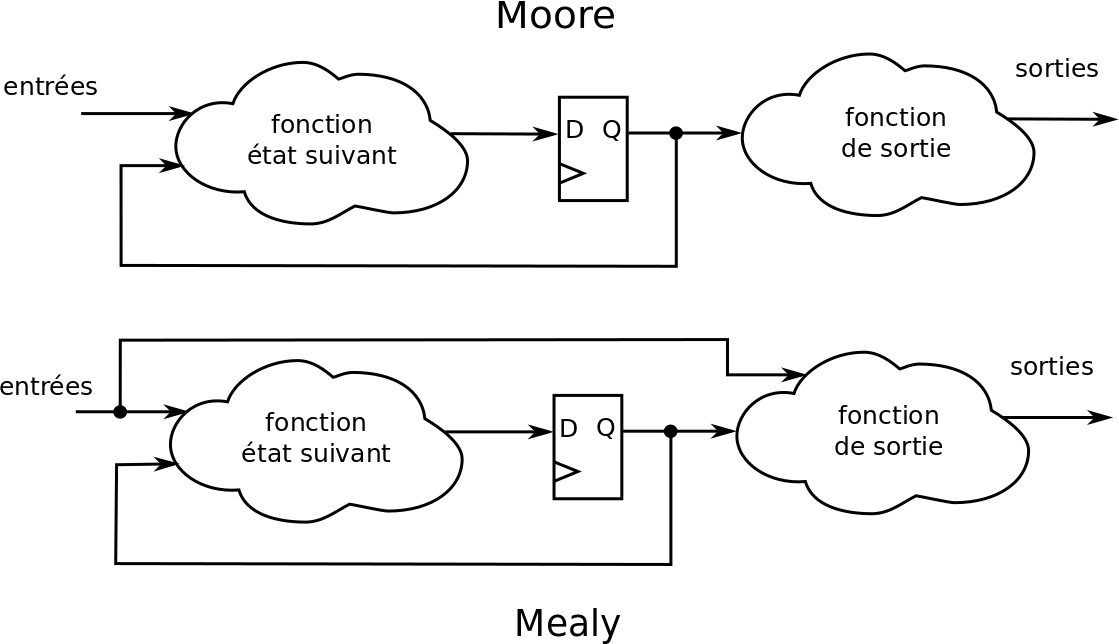
\includegraphics[scale=0.20]{./images/moore_mealy.png}
    %\caption{Automates de Moore et de Mealy}
    %\label{fig:mealy_moore}
  \end{figure}
  \begin{alertblock}{Warnings}
    \begin{itemize}
      \item Composer (i.e interconnecter) des automates de Mealy est \textbf{dangereux}.
      \item Création potentielle de \textbf{boucles combinatoires} : \color{red}{interdit}
    \end{itemize}
  \end{alertblock}
\end{frame}

\begin{frame}{Concevoir un circuit : du diagramme au circuit}
  Un problème de conception d'automate peut se résumer de la manière suivante :
  \begin{enumerate}
    \item Formulation du problème $\rightarrow$ diagramme états-transitions.
    \item Vérification de la {\it causalité} de l'automate décrit.
    \item Encodage des états.
    \item Construction du tableau de séquencement (si nécessaire)
    \item Détermination des fonctions d'état suivant (fonction de transition) et sorties.
  \end{enumerate}

  \begin{figure}[h!]
    \centering
    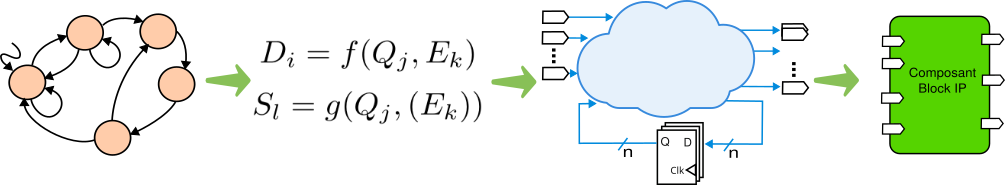
\includegraphics[scale=0.5]{./images/diag_2.png}
    \label{fig:mealy_moore}
  \end{figure}
\end{frame}

\begin{frame}{Vérification de causalité d'un automate}
  \vspace{0.4cm}
  \begin{columns}
    \begin{column}{0.75\textwidth}
      Pour qu'un automate soit considéré comme consistant ou {\it causal}, on doit examiner les conditions $c_i(s)$ des transitions
      partant de chaque état $s\in Q$.
      \begin{itemize}
        \item \textbf{Réactivité} Les conditions sur les transitions doivent être {\it collectivement exhaustives} : il existe forcément une transition à '1'.
        $$\forall s \in Q : \sum_i c_i(s)=1$$
        \item \textbf{Déterminisme} Les conditions sur les transitions doivent être {\it mutuellement exclusives} : on ne peut pas avoir deux transitions à '1' en même temps.
        $$\forall s \in Q, \forall (i,j), i\neq j : c_i(s).c_j(s)=0$$
      \end{itemize}
    \end{column}
    \begin{column}{0.25\textwidth}
      \begin{figure}[h!]
        \centering
        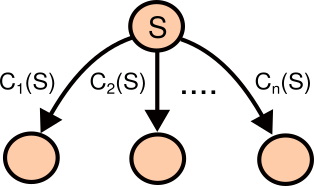
\includegraphics[scale=0.35]{./images/stg_1.png}
      \end{figure}
    \end{column}
  \end{columns}

  \begin{alertblock}{Retenir}
    Cela signifie simplement que dans un état, il existe un, et un seul, état suivant.
  \end{alertblock}

  Notons qu'un état peut avoir comme état suivant lui-même.\\
\end{frame}


\begin{frame}{Etude de cas : vending machine (distributeur)}
  \begin{columns}
    \begin{column}{0.5\textwidth}
      \textbf{Objectif}
      On cherche à réaliser un dispositif qui délivre un objet (cannette etc), après que l'on y a introduit 15 centimes.
      Ces 15 centimes peuvent être introduits à l'aide de pièces de 5 (N) ou 10 centimes (D). La machine ne rend pas la monnaie.
    \end{column}
    \begin{column}{0.5\textwidth}
      \begin{figure}[h]
        \centering
        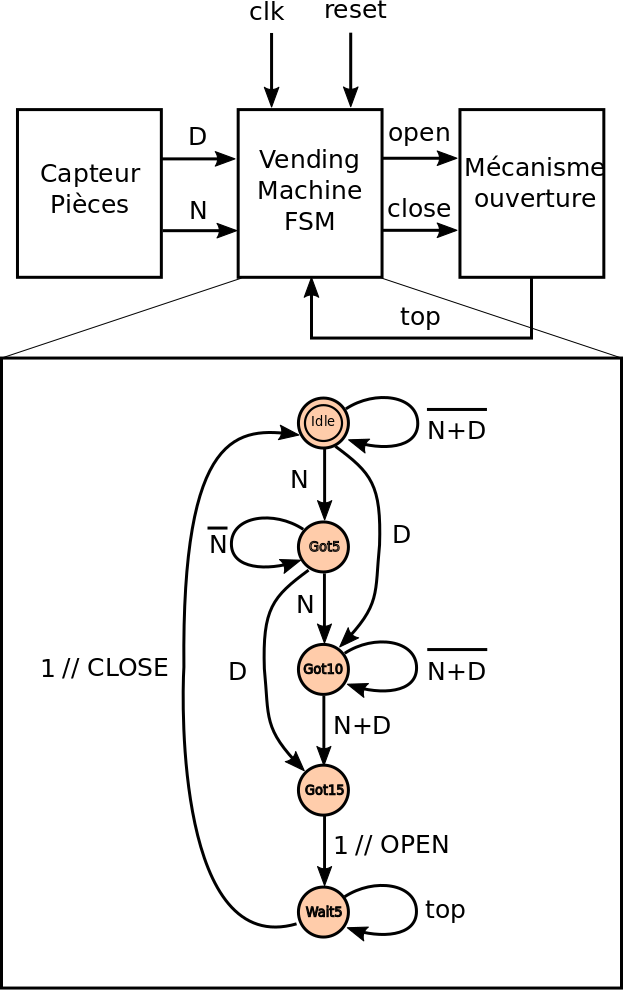
\includegraphics[scale=0.2]{./images/vending_machine.png}
        %\caption{Vending machine et son environnement}
        \label{fig:vending_machine}
      \end{figure}
    \end{column}
  \end{columns}
\end{frame}

\begin{frame}{Etude de cas : encodage des états}
L'encodage des états consiste à associer un code binaire à chaque nom symbolique des états.
  \begin{itemize}
    \item Une infinité d'encodages sont possibles.
    \item Chaque encodage conduit évidemment à des circuits différents structurellement, mais leur comportement
    aux entrées-sorties est identique.
    \item On retiendra \textbf{deux encodages particuliers} :
    \begin{enumerate}
      \item Encodage \textbf{dense} : numérotation binaire classique. Pour $n$ états $\rightarrow$ $\lceil \log_2(n) \rceil$ bits.
      \item Encodage \textbf{"one-hot"} : \textbf{1 bit par état}. $1,2,4,8,16,32,...$. $n$ états $\rightarrow$ $n\rceil$ bits.
    \end{enumerate}
    \item L'encodage "one-hot" permet d'éviter les tableaux de Karnaugh.
  \end{itemize}
\end{frame}

\begin{frame}{Etude de cas : Encodage dense}

  \begin{minipage}{0.4\textwidth}

    \begin{figure}[h]
      \centering
      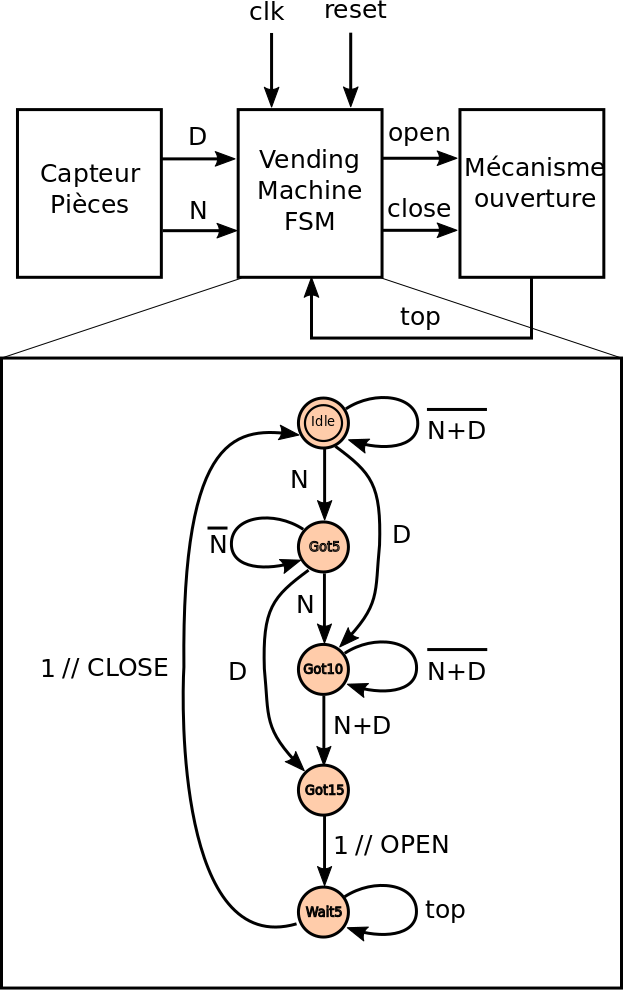
\includegraphics[scale=0.18]{./images/vending_machine.png}
      %\caption{Vending machine et son environnement}
      \label{fig:vending_machine}
    \end{figure}
  \end{minipage}
  \begin{minipage}{0.4\textwidth}
    \begin{table}
      \centering
      Encodage dense :
      \begin{tabular}{|l|c|c|}
            \hline
            état  & numéro & code binaire  \\ \hline \hline
            Idle  & 0      & 000           \\ \hline
            Got5  & 1      & 001           \\ \hline
            Got10 & 2      & 010           \\ \hline
            Got15 & 3      & 011           \\ \hline
            Wait5 & 4      & 100           \\ \hline
        \end{tabular}
    \end{table}
  \end{minipage}


\end{frame}

\begin{frame}{Etude de cas : encodage "one-hot" (1 bit par état)}
  \begin{minipage}{0.4\textwidth}

    \begin{figure}[h]
      \centering
      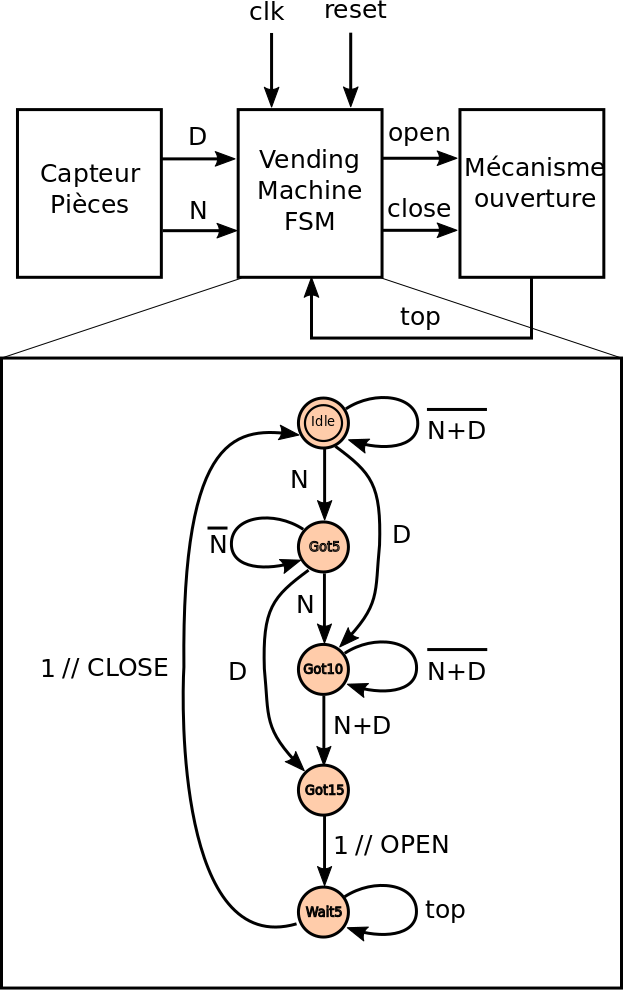
\includegraphics[scale=0.18]{./images/vending_machine.png}
      %\caption{Vending machine et son environnement}
      \label{fig:vending_machine}
    \end{figure}
  \end{minipage}
  \begin{minipage}{0.4\textwidth}
    \begin{table}[!htbp]
      \centering
      Encodage "one-hot" :
      \begin{tabular}{|l|c|c|}
            \hline
            état  & numéro & code binaire  \\ \hline \hline
            Idle  & 1       & 00001           \\ \hline
            Got5  & 2       & 00010           \\ \hline
            Got10 & 4       & 00100           \\ \hline
            Got15 & 8       & 01000           \\ \hline
            Wait5 & 16      & 10000           \\ \hline
        \end{tabular}
    \end{table}
  \end{minipage}
\end{frame}

\begin{frame}{Etude de cas : table de séquencement}
  Le but est de trouver les équations :   $$ D_i=f(Q_j,E_k) $$
    $$ S_l=g(Q_j,(E_k)) $$


Dans un premier temps on conserve les noms des états symboliques.
{\footnotesize
\begin{table}[!htb]
  \centering

  \begin{tabular}{|c|c|c|c||c|c|c|c|}
        \hline
        \cellcolor{blue!25} état courant & $e_1$ & ... & $e_n$ &  \cellcolor{red!25} état suivant & $s_1$ & ... & $s_n$ \\ \hline
        IDLE        & ~    & ~     & ~            & ~            & ~        & ~   & ~    \\ \hline
        \dots       & ~    & ~     & ~            & ~            & ~        & ~   & ~    \\ \hline
        GOT5        & ~    & ~     & ~            & ~            & ~        & ~   & ~    \\ \hline
        \dots       & ~    & ~     & ~            & ~            & ~        & ~   & ~    \\ \hline
    \end{tabular}
\end{table}
}

Puis on utilise l'encodage explicitant les $Q_i$ (état courant) et $D_i$ (état futur).
{\footnotesize
\begin{table}[!htb]
  \centering
    \begin{tabular}{|c|c|c|c|c|c||c|c|c|c|c|c|}
        \hline
        \cellcolor{blue!25}$Q_n$ & \cellcolor{blue!25}\dots & \cellcolor{blue!25} $Q_0$ &  $e_1$ & ... & $e_n$ & \cellcolor{red!25}$D_1$ & \cellcolor{red!25}\dots & \cellcolor{red!25}$D_0$ & $s_1$ & ... & $s_n$ \\ \hline
        ~   & ~    & ~  & ~  & ~  & ~  & ~  & ~  & ~        & ~   & ~ & ~        \\
        ~   & ~    & ~  & ~  & ~  & ~  & ~  & ~  & ~        & ~   & ~ & ~        \\
        \hline
    \end{tabular}
\end{table}
}
\textbf{Equations finales : }
Il reste à observer les colonnes des $D_i$ et $s_j$ et déduire les équations logiques
  \begin{itemize}
    \item Déduction immédiate dans certains cas.
    \item Construction des tableaux de Karnaugh pour chaque $D_i$ et $s_j$
  \end{itemize}
\end{frame}

%
% \begin{frame}{Bascule D : Reset et Set \textit{asynchrones}}
% \begin{columns}
%   \begin{column}{0.45\textwidth}
%     \begin{block}{Cas du \texttt{Reset} : mise à 0}
%       \begin{itemize}
%         \item Le \texttt{reset} est \textbf{prioritaire} sur l'horloge.
%         \item Lorsqu'il est activé $\rightarrow Q=0$
%       \end{itemize}
%     \end{block}
%     \begin{exampleblock}{Cas du \texttt{Set} : mise à 1}
%       \begin{itemize}
%         \item Le \texttt{set} est \textbf{prioritaire} sur l'horloge.
%         \item Lorsqu'il est activé $\rightarrow Q=1$
%       \end{itemize}
%     \end{exampleblock}
%     En cas d'ordres contradictoires $\rightarrow$ voire doc constructeur.
%
%   \end{column}
%   \begin{column}{0.45\textwidth}
%     \centering
%     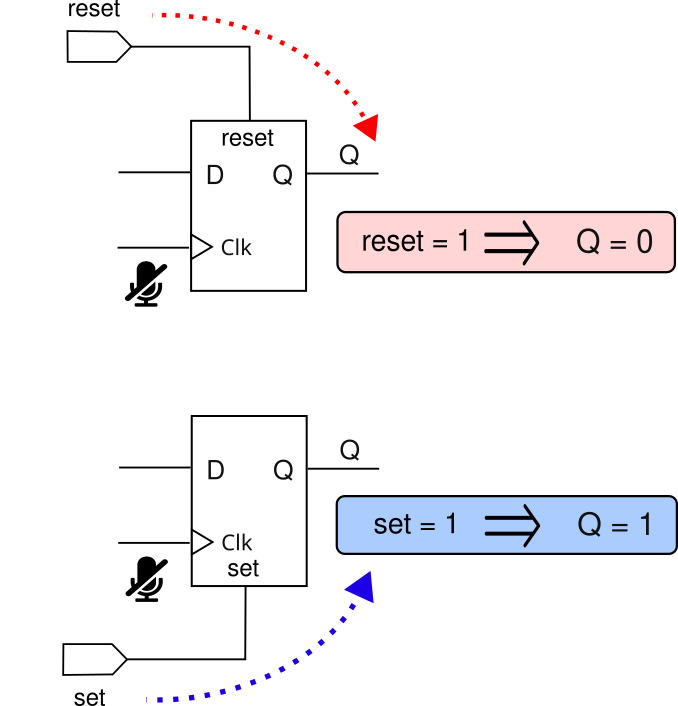
\includegraphics[scale=0.4]{./images/reset_0.png}
%   \end{column}
% \end{columns}
% \end{frame}
%
% \begin{frame}{Bascule D : Reset et Set \textit{asynchrones}}
% \begin{columns}
%   \begin{column}{0.40\textwidth}
%     \centering
%     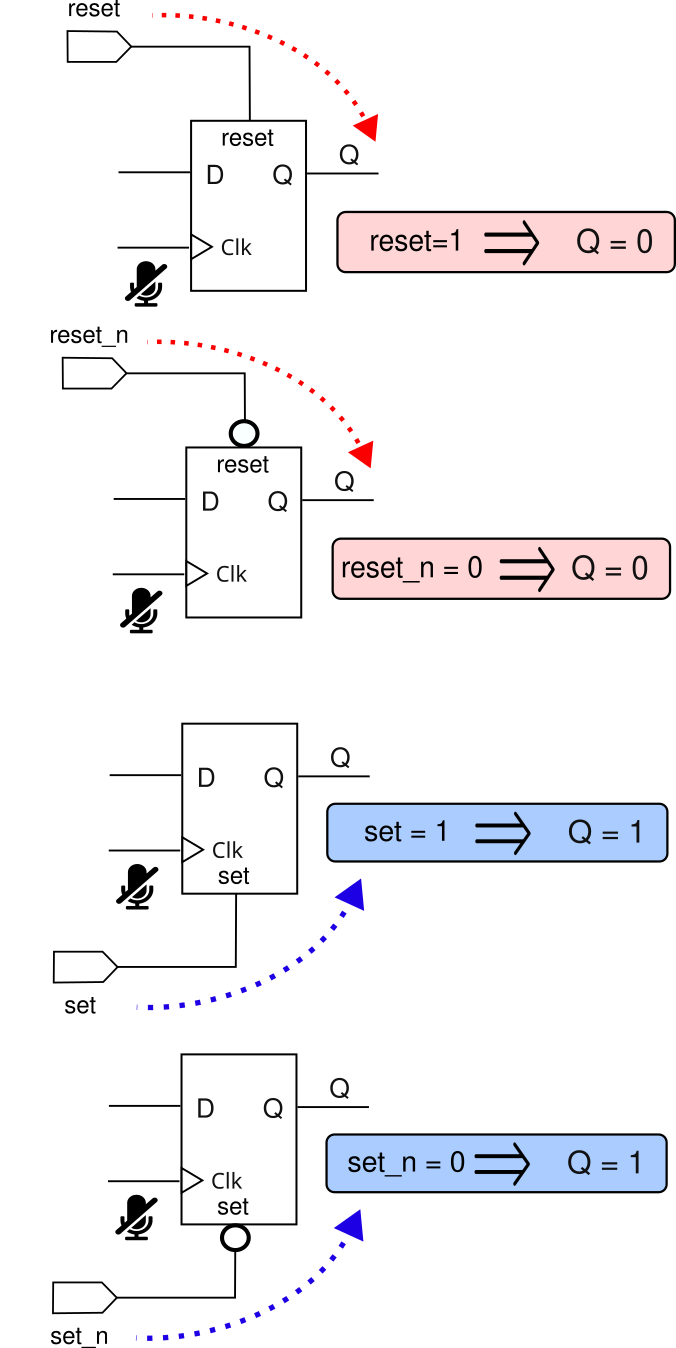
\includegraphics[scale=0.21]{./images/reset_1.png}
%   \end{column}
%   \begin{column}{0.55\textwidth}
%     \begin{block}{Polarité d'activation}
%       \begin{itemize}
%         \item  Les deux signaux \texttt{reset} et \texttt{set} ont eux-mêmes une valeur où ils sont
%         actifs.
%         \item Cette valeur est précisée dans le schéma de la bascule :
%         \begin{itemize}
%           \item Cerle ° indique la \fbox{polarité \texttt{0} active}.
%           \item L'\underline{absence de cercle} ° indique la \fbox{polarité \texttt{1} active}.
%         \end{itemize}
%         \item Cette valeur \textit{peut} être précisée dans le \textit{nommage} du signal :
%         \begin{itemize}
%           \item \texttt{reset\_n} indique une polarité \texttt{0} active.
%           \item \texttt{reset} indique une polarité \texttt{1} active.
%         \end{itemize}
%       \end{itemize}
%     \end{block}
%     \begin{itemize}
%       \item Les noms des signaux dépendent des \textit{conventions de nommage} propres aux entreprises.
%       \item \textbf{Attention : } bien connecter \textbf{tous} les \texttt{reset} et \texttt{set}.
%     \end{itemize}
%   \end{column}
% \end{columns}
% \end{frame}

\begin{frame}{Cas d'étude : automate \texttt{ABC}}
    \begin{columns}
        \begin{column}{0.5\textwidth}

            \begin{center}
              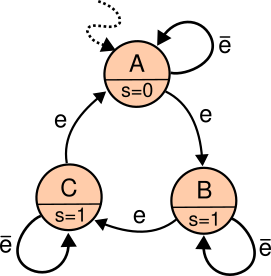
\includegraphics[scale=0.35]{./images/diag_5.png}
            \end{center}
            \centering
            \vspace{0.2cm}

            \begin{tabular}{|c|c||c|c|}
                \hline
                \textbf{État courant} & \(e\) & {\textbf{État futur}} & \(S\) \\
                \hline
                A & 0 & A & 0 \\
                A & 1 & B & 0 \\ \hline
                B & 0 & B & 1 \\
                B & 1 & C & 1 \\ \hline
                C & 0 & C & 1 \\
                C & 1 & A & 1 \\
            \hline
            \end{tabular}
        \end{column}

        \begin{column}{0.5\textwidth}
            \centering
            \textbf{Encodage} : A $\leftrightarrow$ \texttt{00},B $\leftrightarrow$ \texttt{01},C $\leftrightarrow$ \texttt{10}
            %\renewcommand{\arraystretch}{1.3}
            \begin{tabular}{|c|c|c||c|c|c|}
                \hline
                \multicolumn{2}{|c|}{\textbf{État courant}} & \textbf{Entrée}
                & \multicolumn{2}{c|}{\textbf{État futur}} & \textbf{Sortie} \\
                \hline
                \(Q_1\) & \(Q_0\) & \(e\) & \(D_1\) & \(D_0\) & \(S\) \\
                \hline
                0 & 0 & 0 & 0 & 0 & 0 \\
                0 & 0 & 1 & 0 & 1 & 0 \\ \hline
                0 & 1 & 0 & 0 & 1 & 1 \\
                0 & 1 & 1 & 1 & 0 & 1 \\ \hline
                1 & 0 & 0 & 1 & 0 & 1 \\
                1 & 0 & 1 & 0 & 0 & 1 \\
            \hline
            \end{tabular}

            \[
              \left\{
              \begin{aligned}
              D_1 &= \overline{Q_1}.Q_0.e+Q_1.\overline{Q_0}.\overline{e}\\
              D_0 &= \overline{Q_1}.\overline{Q_0}.e + \overline{Q_1}.Q_0.\overline{e}\\
              S   &= Q_1 \oplus Q_0\\
              \end{aligned}
              \right.
            \]

            Il nous manque une technique pour faire mieux : les \textbf{Don't care}
        \end{column}
    \end{columns}
\end{frame}

\begin{frame}{Techniques des \textbf{Don't cares} : profiter des indéterminations}
  \begin{block}{Don't cares}
    \begin{itemize}
      \item Cas manquants, non-applicables $\rightarrow$ sources d'optimisations booléennes.
      \item Présentés comme des \textbf{valeurs libres} '\texttt{X}' (ou '\texttt{-}') dans le tableau de Karnaugh.
    \end{itemize}
  \end{block}

  \begin{columns}
      \begin{column}{0.55\textwidth}
        \begin{tabular}{|c|c|c||c|c|c|}
                \hline
                \multicolumn{2}{|c|}{\textbf{État courant}} & \textbf{Entrée}
                & \multicolumn{2}{c|}{\textbf{État futur}} & \textbf{Sortie} \\
                \hline
                \(Q_1\) & \(Q_0\) & \(e\) & \(D_1\) & \(D_0\) & \(S\) \\
                \hline
                0 & 0 & 0 & 0 & 0 & 0 \\
                0 & 0 & 1 & 0 & 1 & 0 \\ \hline
                0 & 1 & 0 & 0 & 1 & 1 \\
                0 & 1 & 1 & 1 & 0 & 1 \\ \hline
                1 & 0 & 0 & 1 & 0 & 1 \\
                1 & 0 & 1 & 0 & 0 & 1 \\ \hline
                1 & 1 & 0 & x & x & x \\
                1 & 1 & 1 & x & x & x \\
            \hline
            \end{tabular}
      \end{column}
      \begin{column}{0.4\textwidth}
        \textbf{D1 :}
        \begin{tabular}{|c|c|c|}
          \hline
          \diagbox{$Q_1Q_0$}{$e$} & 0 & 1 \\
          \hline
          00 & ~ & ~ \\
          \hline
          01 & ~ & \cellcolor{blue!25}1 \\
          \hline
          11 & \cellcolor{red!30}x & \cellcolor{blue!25}x \\
          \hline
          10 & \cellcolor{red!30}1 & ~ \\
          \hline
        \end{tabular}\\

        \textbf{D0 :}
        \begin{tabular}{|c|c|c|}
          \hline
          \diagbox{$Q_1Q_0$}{$e$} & 0 & 1 \\
          \hline
          00 & ~ & 1 \\
          \hline
          01 & \cellcolor{red!30}1 & ~ \\
          \hline
          11 & \cellcolor{red!30}x & x \\
          \hline
          10 & ~ & ~ \\
          \hline
        \end{tabular}
      \end{column}
  \end{columns}
\end{frame}

\begin{frame}{Cas d'étude : automate \texttt{ABC}}
  \begin{columns}
    \begin{column}{0.4\textwidth}
      \textbf{Diagramme états-transitions}
      \begin{center}
        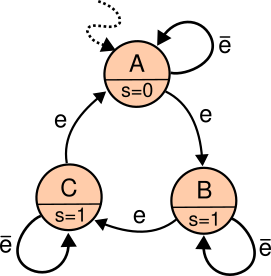
\includegraphics[scale=0.35]{./images/diag_5.png}
      \end{center}

      \textbf{Equations constitutives :}
      \begin{itemize}
        \item Choix : encodage dense
        \item Longs calculs...
      \end{itemize}
      \[
        \left\{
          \begin{aligned}
          D_1 &= Q_0.e+Q_1.\overline{e}\\
          D_0 &= Q_0.\overline{e}+ \overline{Q_1}.\overline{Q_0}.e \\
          S   &= Q_1 \oplus Q_0\\
          \end{aligned}
          \right.
      \]
    \end{column}
    \begin{column}{0.6\textwidth}
      \textbf{Circuit numérique}
      \begin{center}
        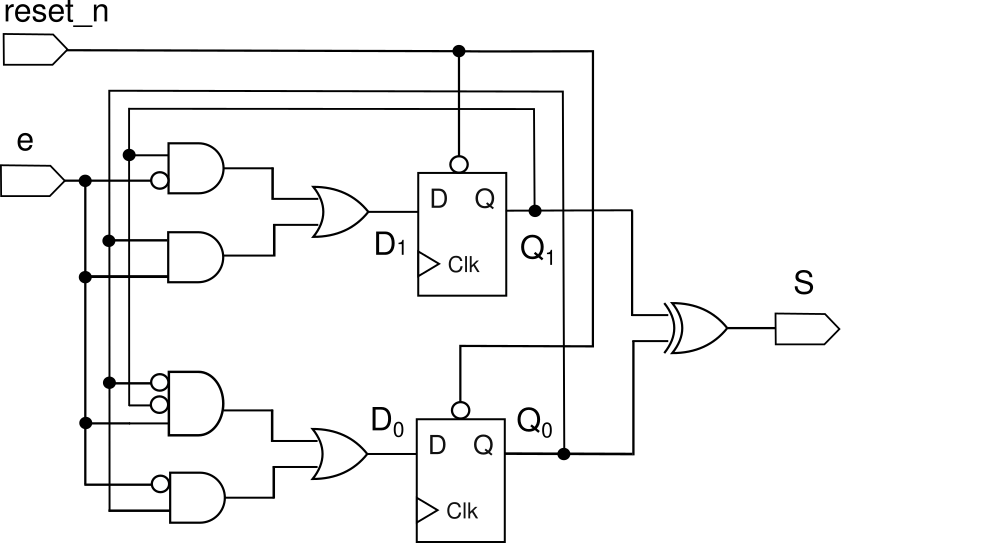
\includegraphics[scale=0.30]{./images/abc.png}
      \end{center}
    \end{column}
  \end{columns}
\end{frame}

\begin{frame}{Cas \textit{Merveilleux} de l'encodage One-Hot}

On peut déduire les équations \textbf{directement} par simple \textbf{lecture} du diagramme états-transitions.

\begin{alertblock}{Principe}
  \begin{itemize}
    \item Cet encodage spécifique signifie qu'\textbf{une seule} bascule $D_i$ présente une sortie $Q_i$ à $1$.
    \item Tout se passe donc comme si un \textbf{jeton} circule d'\textbf{une bascule à l'autre}.
    \item Savoir quelle bascule "détient le jeton" suffit à connaître l'état courant.
  \end{itemize}
\end{alertblock}

\textbf{Application directe} du schéma de traduction suivant :
\begin{columns}
  \begin{column}{0.5\textwidth}
    \begin{figure}[!htp]
      \centering
      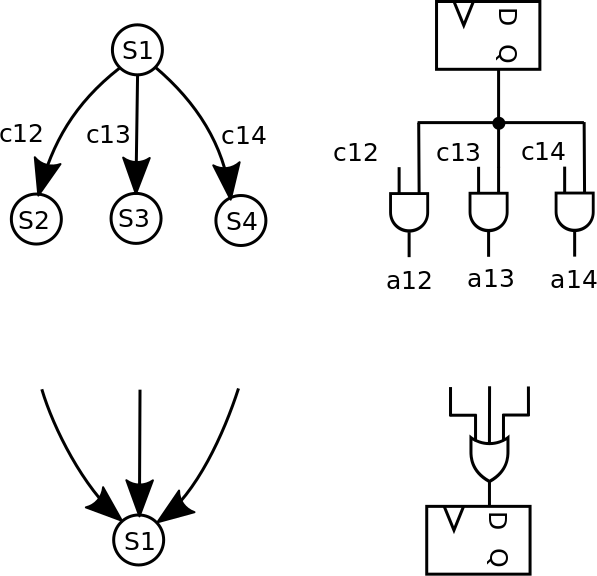
\includegraphics[scale=0.16]{./images/one_hot_method.png}
      %\caption{Procédé simplifiant la génération d'un circuit d'automate dans le cas d'un encodage {\it one-hot}.}
      \label{fig:one_hot}
    \end{figure}
  \end{column}

  \begin{column}{0.5\textwidth}
    \begin{equation*}
      \begin{cases}
        d_2=q_1.c_{12}+\dots \\
        d_3=q_1.c_{13}+\dots \\
        d_4=q_1.c_{14}+\dots \\
        d_1=\dots + \dots + \dots \\
      \end{cases}
    \end{equation*}
  \end{column}
\end{columns}
\end{frame}

%================================================================
\begin{frame}{Encodage one-hot : exemple sur l'automate \texttt{ABC}}
  \begin{columns}
    \begin{column}{0.5\textwidth}
      \centering
      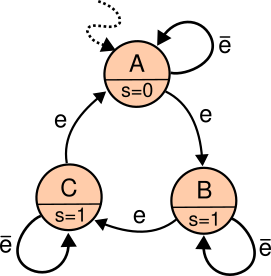
\includegraphics[scale=0.35]{./images/diag_5.png}
      \begin{itemize}
        \item Application du schéma de traduction :
      \end{itemize}
      \begin{columns}
        \begin{column}{0.5\textwidth}
          \begin{figure}[!htp]
            \centering
            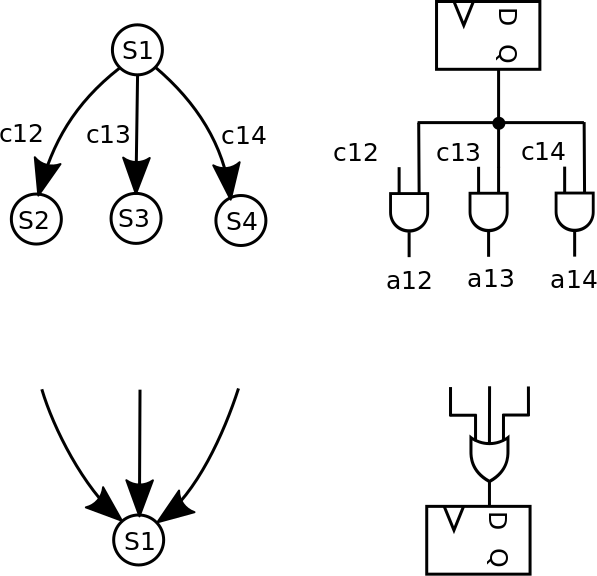
\includegraphics[scale=0.12]{./images/one_hot_method.png}
            %\caption{Procédé simplifiant la génération d'un circuit d'automate dans le cas d'un encodage {\it one-hot}.}
            \label{fig:one_hot}
          \end{figure}
        \end{column}

        \begin{column}{0.5\textwidth}
          \begin{equation*}
            \begin{cases}
              D_0=Q_0.\overline{e}+Q_2.e \\
              D_1=Q_1.\overline{e}+Q_0.e  \\
              D_2=Q_2.\overline{e}+Q_1.e  \\
              S=Q_1 + Q_2\\
            \end{cases}
          \end{equation*}
          {\scriptsize Note : le calcul de \texttt{S} est hors schéma.}
        \end{column}
      \end{columns}
    \end{column}
    \begin{column}{0.5\textwidth}
      \begin{figure}[!htp]
        \centering
        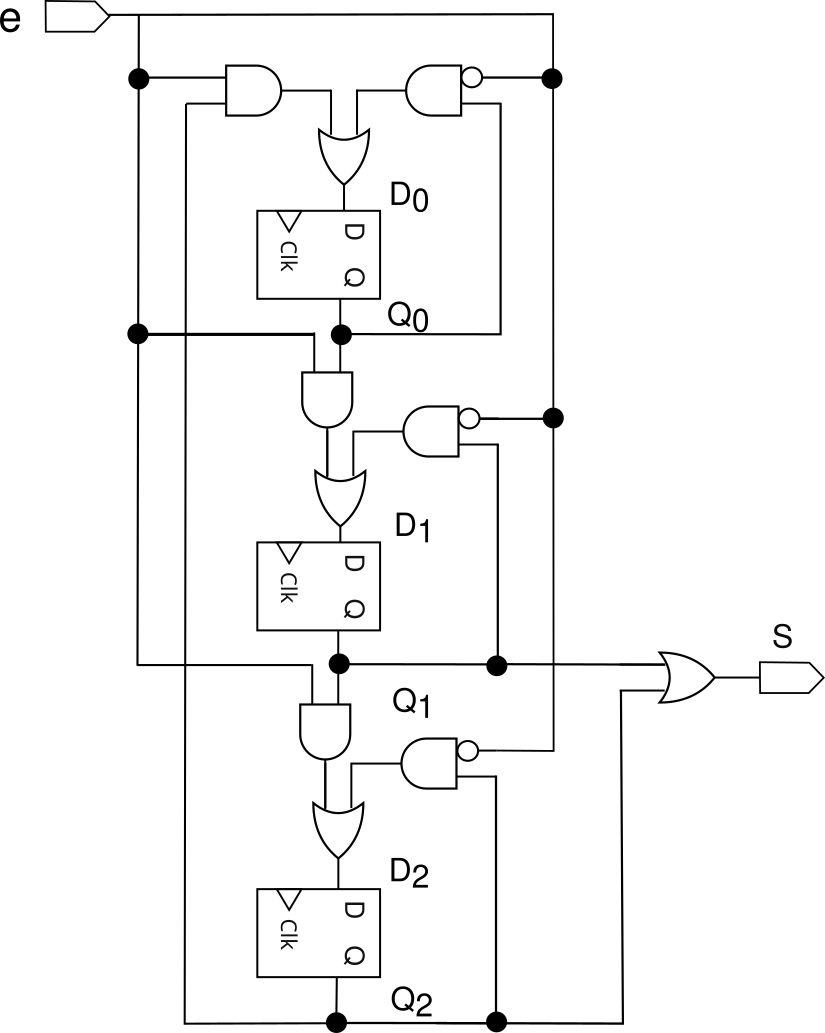
\includegraphics[scale=0.22]{./images/abc_one_hot.png}
        %\caption{Procédé simplifiant la génération d'un circuit d'automate dans le cas d'un encodage {\it one-hot}.}
        %\label{fig:one_hot}
      \end{figure}
    \end{column}
  \end{columns}
\end{frame}

\begin{frame}{Encodage one-hot : exemple sur l'automate \texttt{ABC}}
  \begin{columns}
    \begin{column}{0.5\textwidth}
      \textbf{Initialisation du circuit : en \color{red}{rouge}}
      \begin{itemize}
        \item Etat initial attendu : $A \rightarrow 001$
        \item Le signal \texttt{reset\_n} est \textbf{actif bas}.
        \begin{itemize}
          \item Nommage "\texttt{\_n}" (convention).
        \end{itemize}
        \item $Q_0$ doit valoir 1 : on utilise la "patte" \texttt{set}.
        \begin{itemize}
          \item ici active à 0 (présence '°' indiquée sur la bascule)
        \end{itemize}
        \item $Q_1$ doit valoir 0 : on utilise la "patte" \texttt{reset}.
        \item $Q_2$ doit valoir 0 : on utilise la "patte" \texttt{reset}.
        \begin{itemize}
          \item ici active à 0 (présence '°' indiquée sur la bascule)
        \end{itemize}
      \end{itemize}
      \textbf{Autres câblages : }
      \begin{itemize}
        \item \textbf{Désactivation} ({\color{blue}{bleu}}) des \texttt{reset} et \texttt{set} inutilisés.
        \item \color{black}Présence de l'horloge en \color{green}{vert}.
        % \item Notez l'absence des signaux d'alimentation des portes logiques.
        % \begin{itemize}
        %   \item Mais cette alimentation existe bien !
        % \end{itemize}
      \end{itemize}
    \end{column}
    \begin{column}{0.5\textwidth}
      \begin{figure}[!htp]
        \centering
        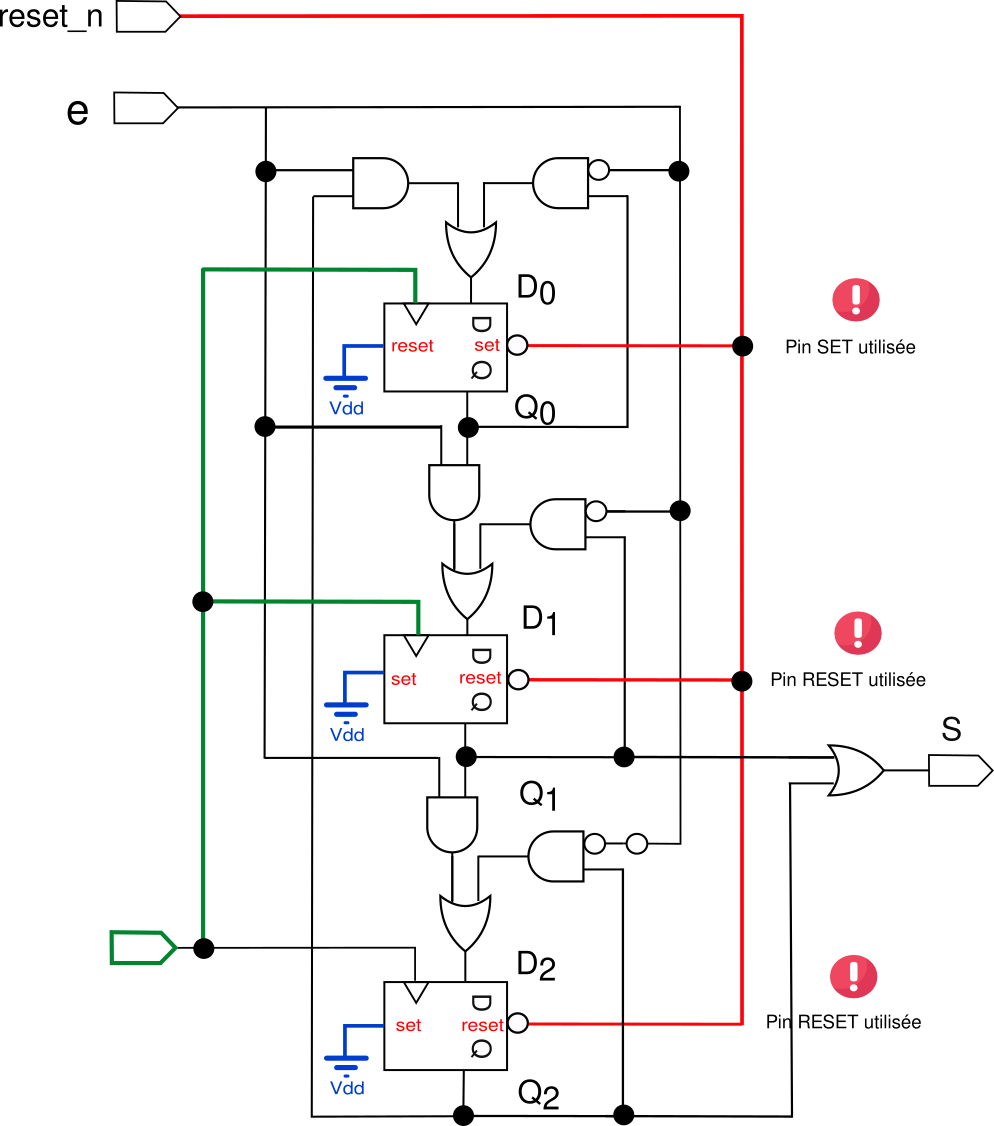
\includegraphics[scale=0.22]{./images/abc_one_hot_reset.png}
        %\caption{Procédé simplifiant la génération d'un circuit d'automate dans le cas d'un encodage {\it one-hot}.}
        %\label{fig:one_hot}
      \end{figure}
    \end{column}
  \end{columns}

\end{frame}

% \begin{frame}{Cas de l'encodage One-Hot}
%
%   \begin{itemize}
%     \item On dessine une bascule $D$ pour un état $S$
%     \item Pour chacune des transitions sortantes d'un état $S_i$ vers un état $S_j$, on dessine une porte AND connectée d'une part à la sortie $Q$ de la bascule de l'état $S_i$, et
%     d'autre part la condition booléenne $c$ de la transition $S_i\rightarrow_{c} S_j$. Appelons $c_{i,j}$ la sortie de cette porte AND.
%     \item Pour chacune des transitions entrantes d'un état $S_j$ on dessine une porte OR connectée à l'entrée $D_j$ et possédant autant d'entrées qu'il existe de transitions entrantes.
%     A partir des états précedents $S_i$, on connecte le signal $c_{i,j}$ sur une des entrées de cette porte OR.
%   \end{itemize}
%
% \end{frame}


\begin{frame}{Rappel}
\begin{itemize}
  \item Dans certains cas simples, il reste possible de dessiner le circuit.
  \item Sinon, on s'en tient au schéma d'ensemble suivant :
\end{itemize}

\begin{figure}[!htp]
  \centering
  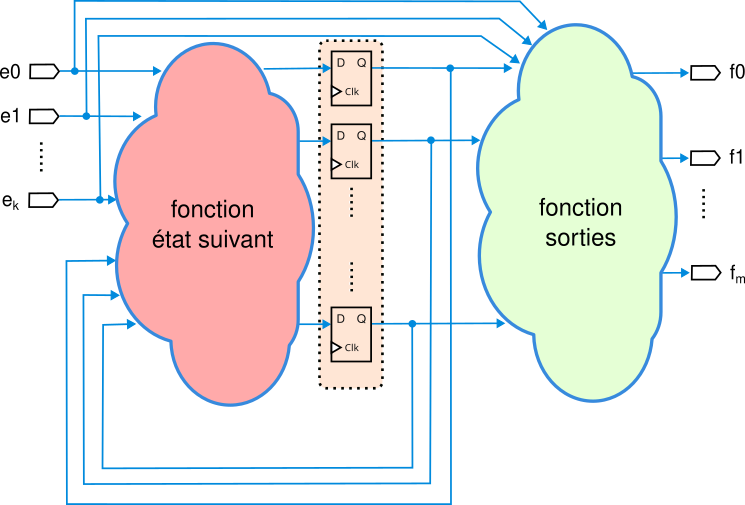
\includegraphics[scale=0.4]{./images/fsm_4.png}
  %\caption{Procédé simplifiant la génération d'un circuit d'automate dans le cas d'un encodage {\it one-hot}.}
  %\label{fig:one_hot}
\end{figure}

\end{frame}

%% \begin{frame}
%   \begin{columns}
%     \begin{column}{0.5\textwidth}
%     \end{column}
%     \begin{column}{0.5\textwidth}
%     \end{column}
%   \end{columns}
% \end{frame}

\begin{frame}{Automate \texttt{ABC} sur FPGA : compléments}
  \begin{columns}
    \begin{column}{0.45\textwidth}
      \begin{itemize}
        \item Synthèse RTL/logique
        \begin{itemize}
          \item outil \texttt{Vivado Xilinx (AMD)}
        \end{itemize}
        \item Adaptation VHDL des interfaces :
        \begin{itemize}
          \item \texttt{switch} en va-et-vient : créé l'événement '\texttt{e}' d'entrée
          \item Affichage 7 segments : états '\texttt{s}' convertit en nibble.
        \end{itemize}
      \end{itemize}
    \end{column}
    \begin{column}{0.55\textwidth}
      \begin{center}
        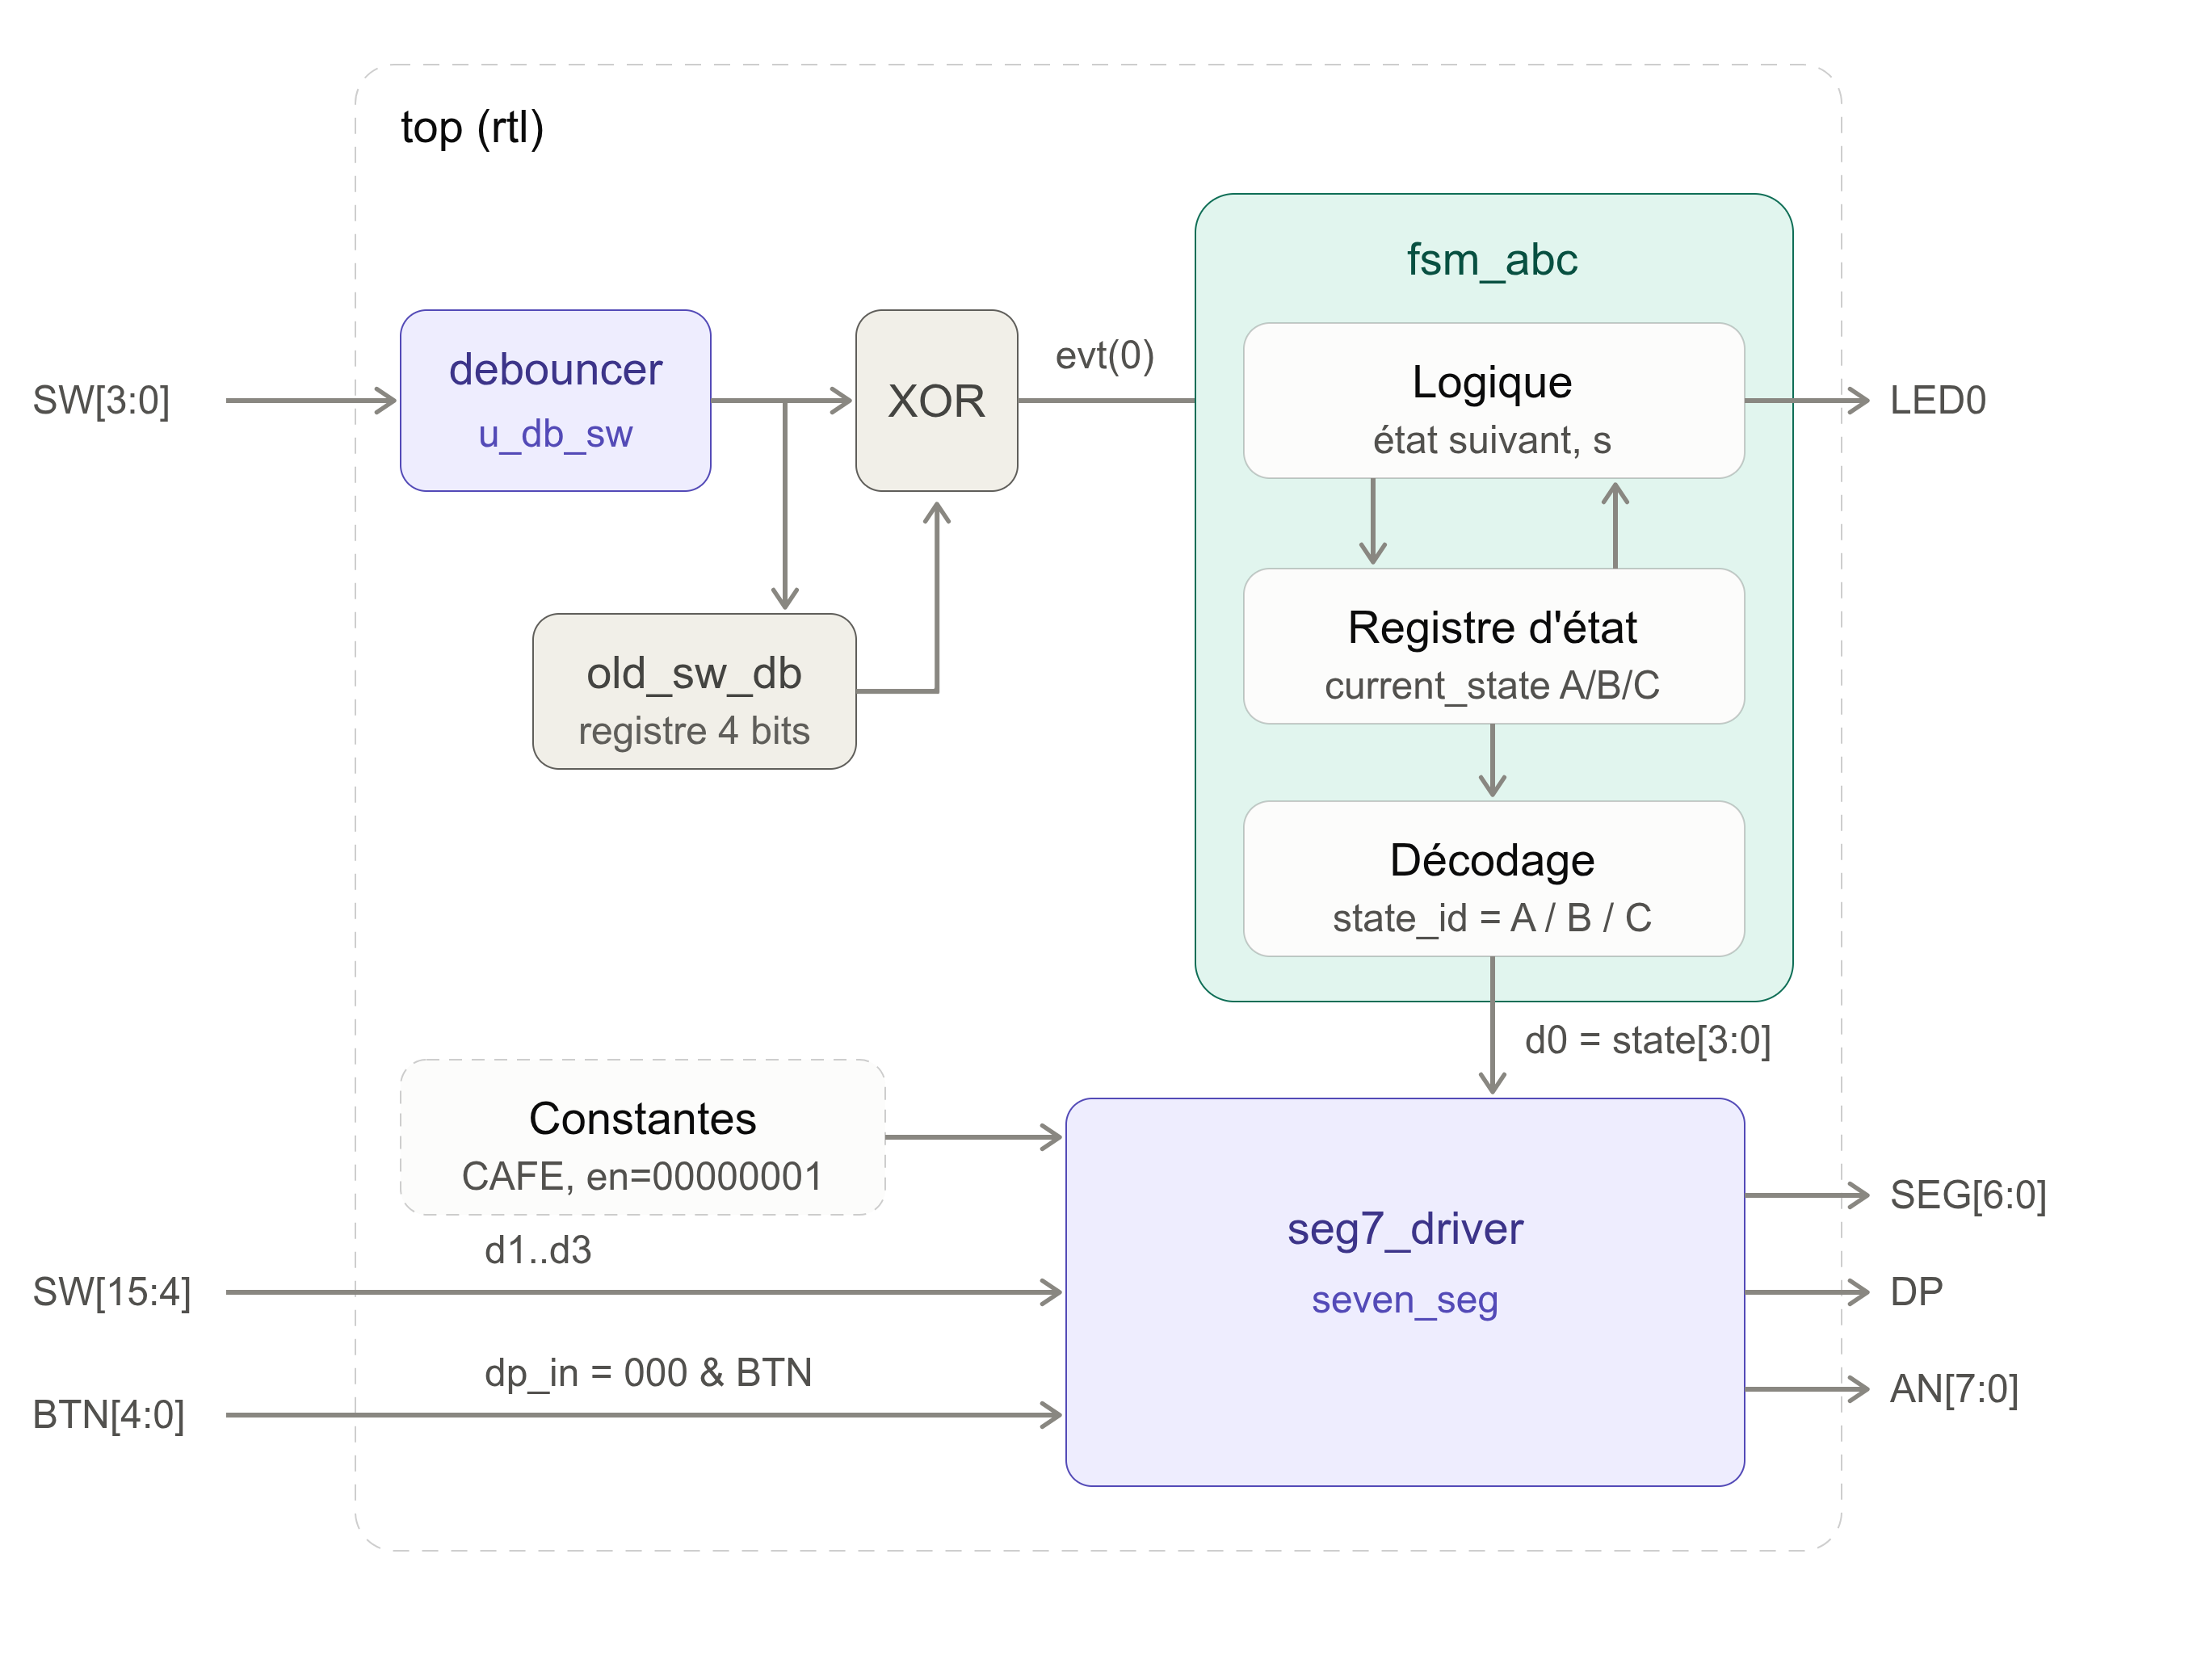
\includegraphics[scale=0.09]{./images/schematic_top_hierarchique.png}
      \end{center}
    \end{column}
  \end{columns}
\end{frame}

\begin{frame}{Composer des systèmes : exemple bi-processeur MIPS}
  Le jeu est désormais de \textbf{composer} des systèmes à partir de \textbf{composants}.
  \begin{itemize}
    \item De plus en plus gros.
    \item Approche récursive, constructive.
  \end{itemize}
  \begin{columns}
    \begin{column}{0.5\textwidth}
      \begin{center}
        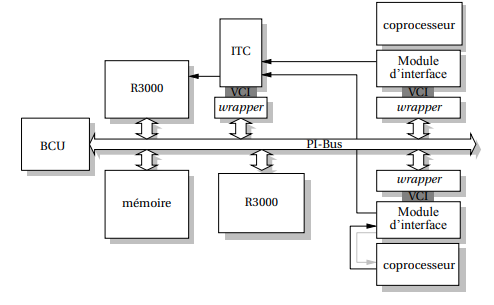
\includegraphics[scale=0.5]{./images/denis_hommais_arch_1.png}
      \end{center}
    \end{column}
    \begin{column}{0.5\textwidth}
      \begin{center}
        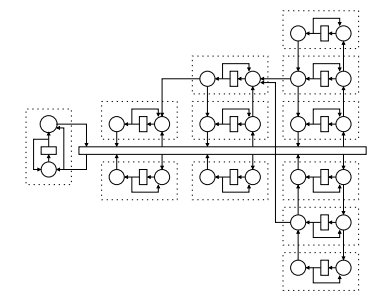
\includegraphics[scale=0.5]{./images/denis_hommais_arch_2.png}
      \end{center}
    \end{column}
  \end{columns}
\end{frame}

%\section{Introduction aux langages de description matériels : VHDL}
%========================================================================================
%
% \section{Initiation aux langages de description matérielle : VHDL}

\begin{frame}{HDL : Hardware description language}
  \begin{itemize}
    \item Les HDL permettent de \textbf{décrire} des systèmes.
    \begin{itemize}
      \item ...de le même manière que \texttt{html} permet de décrire le contenu d'une page web.
    \end{itemize}
    \item Ils sont donc très différents des langages de programmation classiques.
  \end{itemize}

  A titre d'exemple, nous donnons ici un code d'un HDL très important en Electronique {\it analogique} : \textbf{Spice}.
  Spice permet de décrire comment les composants usuels (résistance, capacité, inductance) sont interconnectés.
  Le simulateur Spice permet de rendre compte du comportement du circuit.
  \textbf{Nous allons procéder de même avec VHDL}, mais à plus haut niveau.
  \begin{figure}[h!]
    \centering
    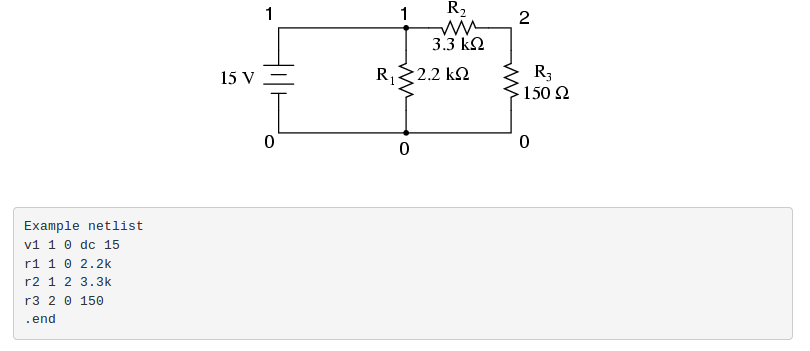
\includegraphics[scale=0.30]{./images/spice.png}
  \end{figure}
\end{frame}

\begin{frame}{Historique de VHDL}
  \begin{itemize}
    \item VHDL est l'acronyme de : VHSIC Hardware Description Language.
    \begin{itemize}
      \item VHSIC : Very High Speed Integrated Circuit
    \end{itemize}
    \item VHDL a été commandé par le Département à la Défense Américaine (DoD).
    \item Sa syntaxe s'inspire fortement d'\textbf{ADA}, très utilisé en \textit{logiciel} dans les années 80.
    \item VHDL est fortement et explicitement \textbf{typé}.
    \item Le but initial était de permettre aux acteurs de la Silicon Valley de seulement échanger des informations/designs de manière cohérente.
    \item Son concurrent direct est le langage \textbf{Verilog}.
    \item VHDL est un langage \textit{réputé difficile}. Il parle de :
    \begin{itemize}
      \item structures qui opèrent en parallèle
      \item signaux
      \item deux formes de temps
    \end{itemize}
  \end{itemize}

  Ces langages sont standardisés par l'IEEE. Plusieurs versions pour VHDL : 87,\textbf{93},08 notamment.
\end{frame}

\begin{frame}{VHDL : Simulation \& Synthèse}
  \begin{columns}
    \begin{column}{0.5\textwidth}
      VHDL est utilisé pour deux activités différentes :
      \begin{itemize}
        \item La \textbf{simulation} : vérification fonctionnelle sur PC, du bon fonctionnement du système décrit.
        \item La \textbf{synthèse} : la génération automatique du système à partir des descriptions.
        \begin{itemize}
          \item Ces descriptions sont de plus en plus abstraites.
          \item On se limitera essentiellement dans ce cours à décrire le circuit en terme d'équations logiques.
          \item Le niveau directement plus abstrait est le niveau RTL.
        \end{itemize}
      \end{itemize}
      \begin{alertblock}{Flot de conception}
        \begin{itemize}
          \item L'ingénierie des systèmes numériques requiert une organisation méticuleuse.
          \item Autant techniquement qu'humainement.
        \end{itemize}
      \end{alertblock}
    \end{column}
    \begin{column}{0.5\textwidth}
      \begin{center}
        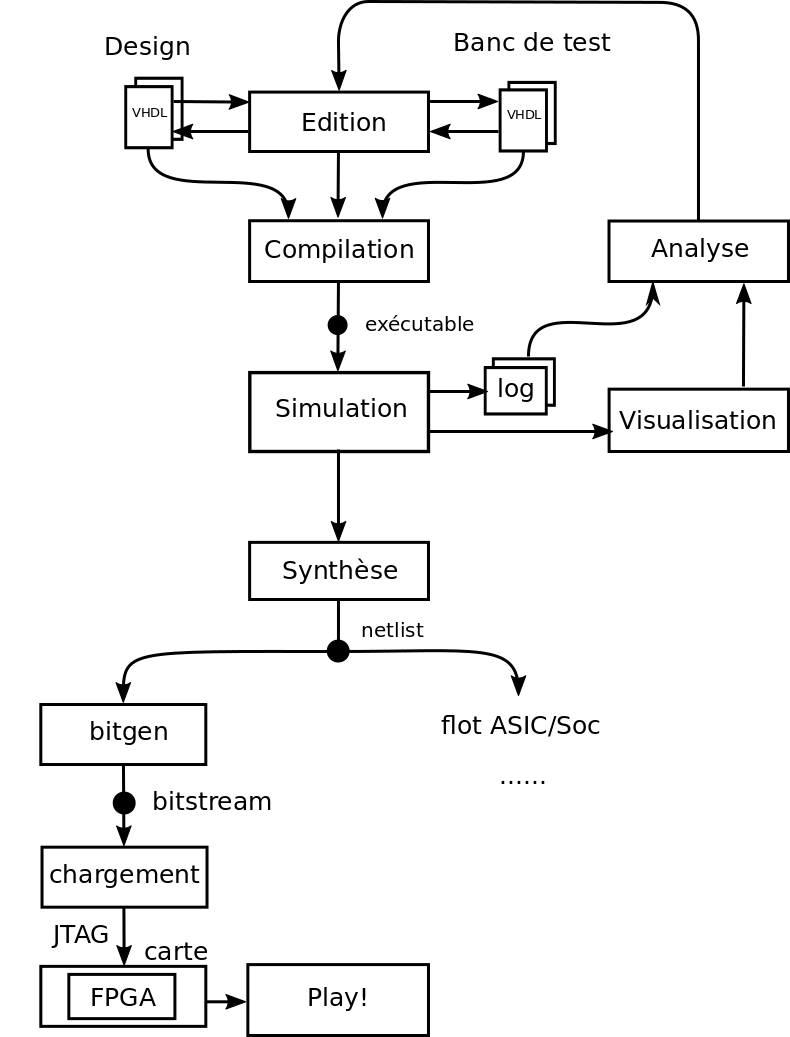
\includegraphics[scale=0.18]{./images/conception_generale.png}
      \end{center}
    \end{column}
  \end{columns}
\end{frame}

% \begin{frame}{Flot général}
% \begin{columns}
%   \begin{column}{0.5\textwidth}
%   \end{column}
%   \begin{column}{0.5\textwidth}
%   \end{column}
% \end{columns}
% \end{frame}

\begin{frame}{Survol de la Simulation VHDL}
  \begin{columns}
    \begin{column}{0.45\textwidth}
      La simulation, réalisée sur PC :
      \begin{itemize}
        \item Repose sur un \textbf{mécanisme d'échéancier} :
        \begin{itemize}
          \item Event-driven simulator.
          \item Image d'une \textit{to-do list}.
        \end{itemize}
        \item Le temps est incrémenté petit-à-petit :
        \begin{itemize}
          \item \textbf{Temps physique} simulé
          \item \textbf{Temps causal} : {\it delta delay/cycles}. Pas infinitésimaux de propagation.
        \end{itemize}
        \item Le simulateur préserve la \textbf{causalité} entre signaux.
        \item C'est une tâche non-triviale pour un programme (simulateur) qui s'exécute sur un ordinateur séquentiel.
      \end{itemize}
    \end{column}
    \begin{column}{0.55\textwidth}
      \begin{center}
        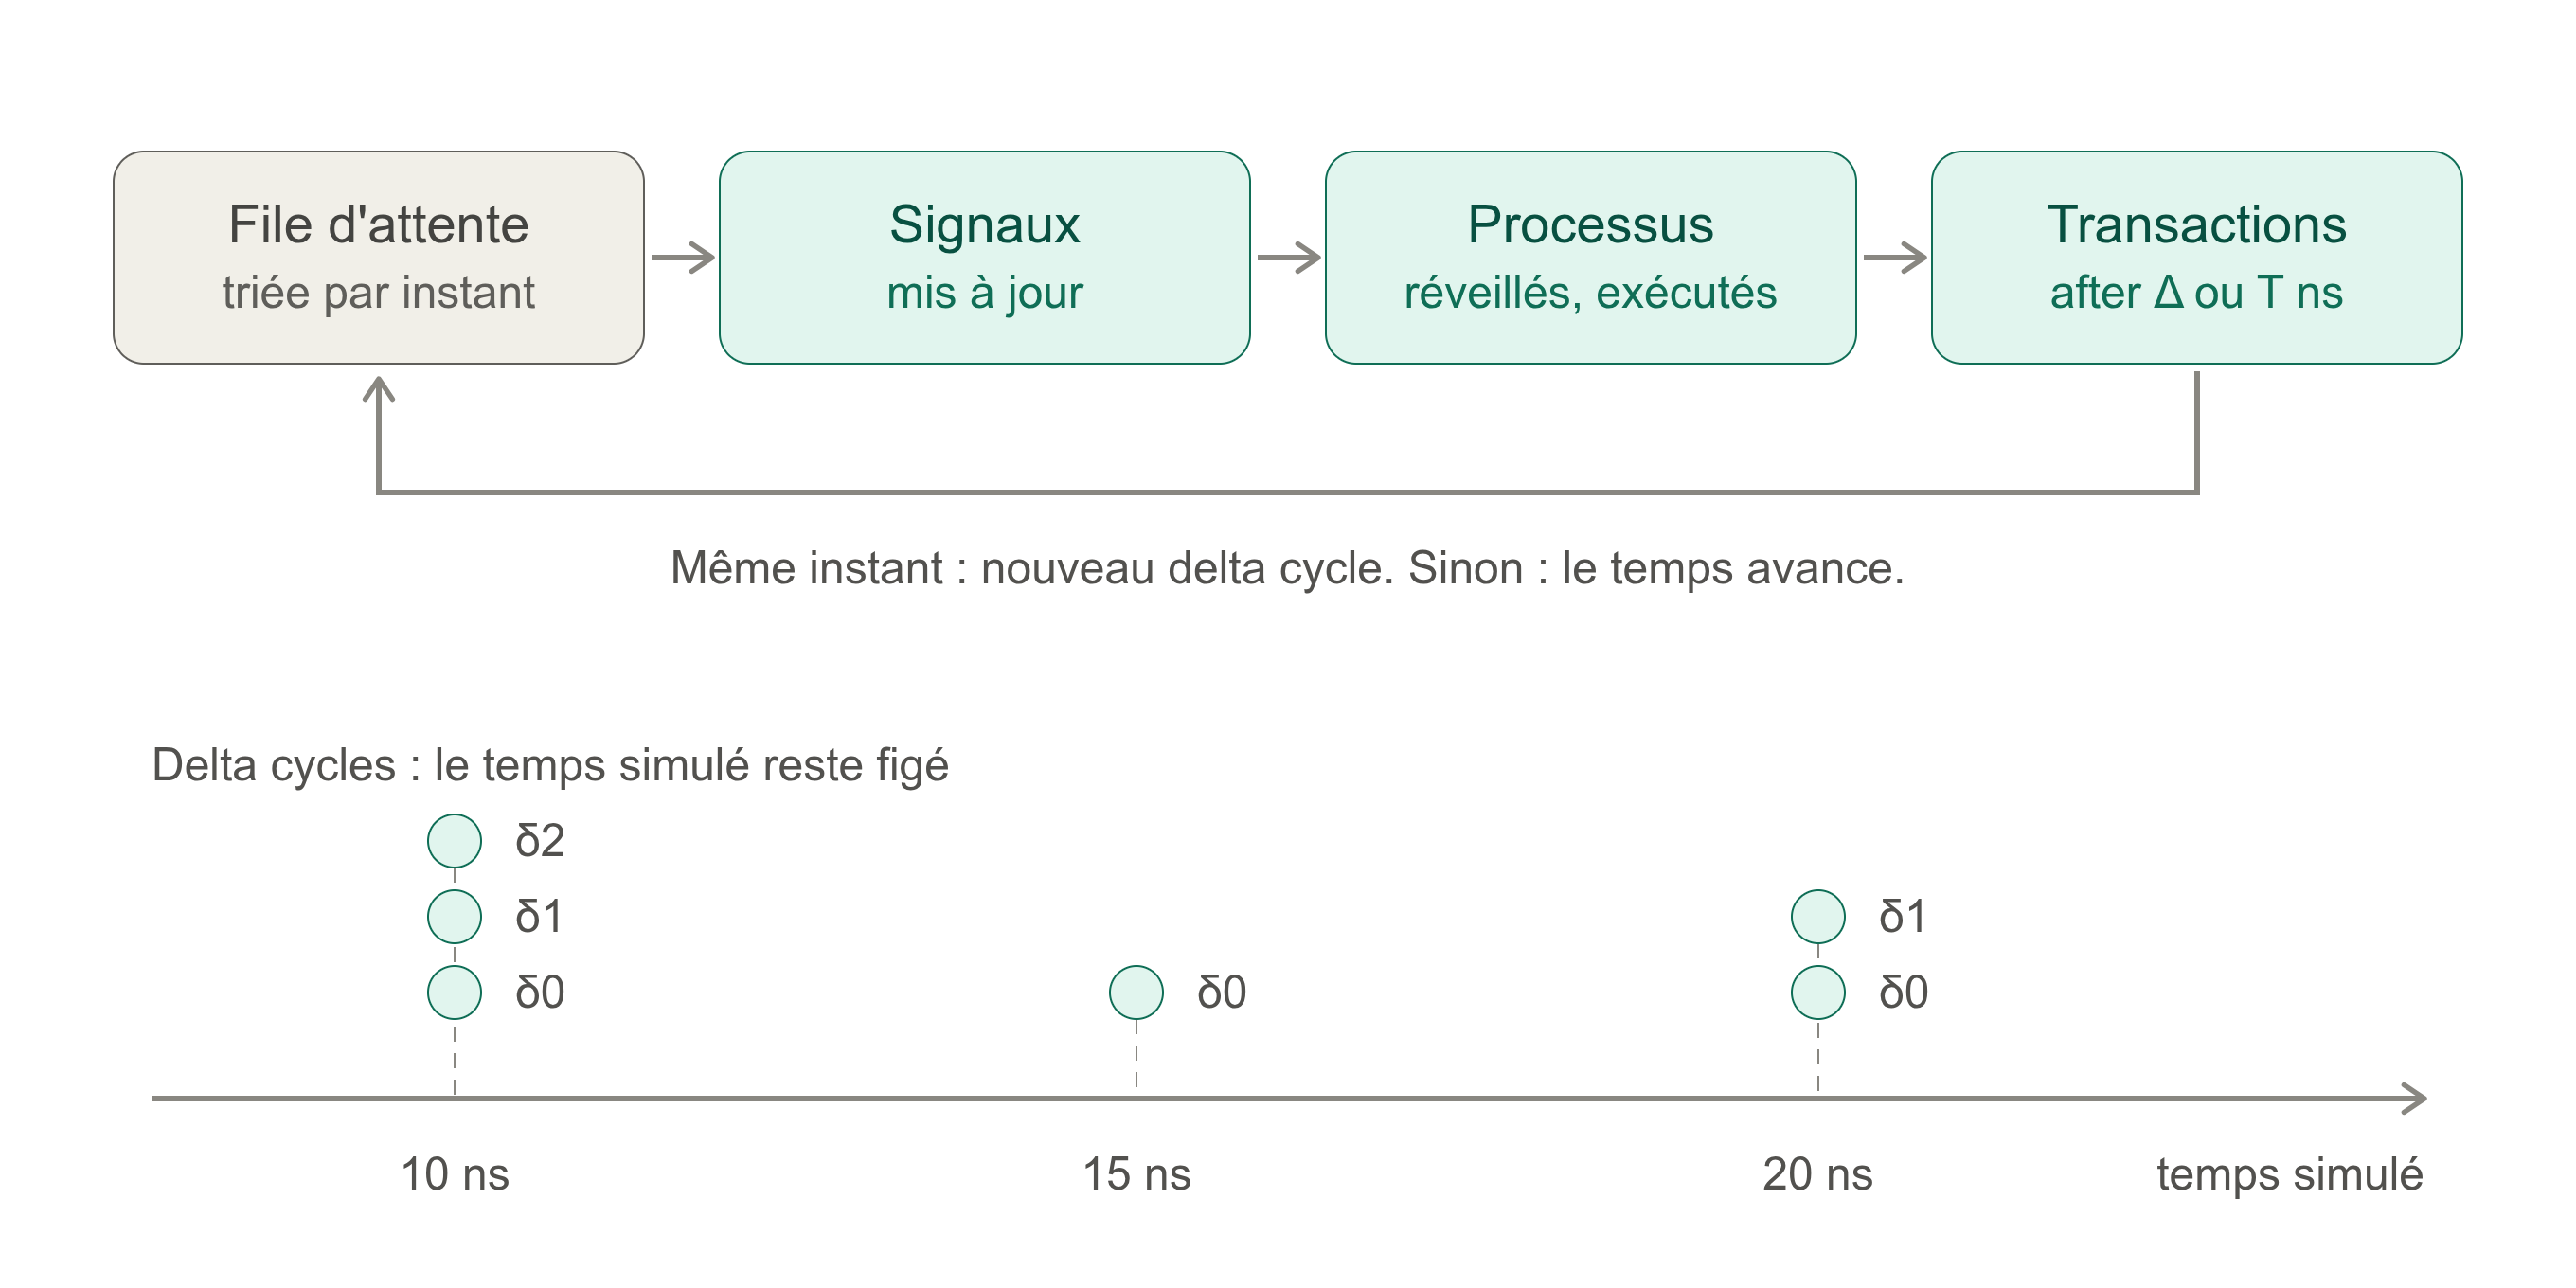
\includegraphics[scale=0.09]{./images/simulation_evenements_discrets_vhdl.png}
      \end{center}
    \end{column}
  \end{columns}
\end{frame}

\begin{frame}{La synthèse logique : du RTL à la netlist mappée}
  \begin{columns}[T,onlytextwidth]

  % ---------- Colonne gauche : explication ----------
  \begin{column}{0.46\textwidth}
    \small
    \textbf{Définition}\\[2pt]
    Transformer une description RTL (VHDL synthétisable) en une
    \emph{netlist} de cellules d'une technologie cible (FPGA ou ASIC).

    \vspace{6pt}
    \textbf{Étapes principales}
    \begin{enumerate}
      \item \textbf{Élaboration} : analyse du code, résolution de la
            hiérarchie, inférence de logique combinatoire et de registres.
      \item \textbf{Optimisation} : minimisation booléenne, partage de
            sous-expressions, suppression de la logique inutile.
      \item \textbf{Mapping technologique} : recouvrement du graphe de portes
            par les cellules du vendeur (LUT, bascules, cellules standard).
    \end{enumerate}

    \vspace{4pt}
    Le mapping est piloté par la \textbf{bibliothèque vendeur} et par les
    \textbf{contraintes} (fréquence, surface, puissance).

    \vspace{4pt}
    \textbf{Résultat} : une netlist mappée, prête pour le placement-routage.
  \end{column}

  % ---------- Colonne droite : schéma ----------
  \begin{column}{0.52\textwidth}
    \centering
    \begin{tikzpicture}[
        scale=0.88, every node/.style={transform shape},
        gbox/.style={draw=gray!70, fill=gray!15, rounded corners=3pt, line width=0.4pt},
        tbox/.style={draw=teal!80!black, fill=teal!15, rounded corners=3pt, line width=0.4pt},
        cell/.style={draw=gray!80, fill=white, rounded corners=1.5pt, line width=0.4pt,
                     font=\scriptsize, inner sep=1pt},
        arr/.style={-{Stealth[length=1.8mm]}, line width=0.7pt},
        wire/.style={line width=0.5pt},
        lbl/.style={font=\footnotesize\bfseries, align=right}
      ]
      % --- RTL ---
      \draw[gbox] (0,0) rectangle (4.2,-1.2);
      \node[font=\footnotesize\bfseries] at (2.1,-0.32) {RTL (VHDL)};
      \node[font=\footnotesize\ttfamily] at (2.1,-0.82) {y <= (a and b) or c;};

      % --- flèche 1 ---
      \draw[arr] (2.1,-1.2) -- (2.1,-2.1);
      \node[lbl, anchor=east] at (1.95,-1.65) {Élaboration};

      % --- Netlist générique ---
      \draw[gbox] (0,-2.1) rectangle (4.2,-4.3);
      \node[font=\footnotesize\bfseries] at (2.1,-2.42) {Netlist générique};
      \node[font=\scriptsize] at (2.1,-2.74) {portes et bascules};
      \node[cell, minimum width=0.8cm, minimum height=0.5cm] (and) at (1.3,-3.35) {AND};
      \node[cell, minimum width=0.8cm, minimum height=0.5cm] (or)  at (2.9,-3.35) {OR};
      \draw[wire] (0.65,-3.23) -- (and.west |- 0,-3.23);
      \draw[wire] (0.65,-3.47) -- (and.west |- 0,-3.47);
      \node[font=\scriptsize] at (0.4,-3.23) {a};
      \node[font=\scriptsize] at (0.4,-3.47) {b};
      \draw[arr] (and.east) -- (or.west);
      \draw[wire] (or.east) -- (3.65,-3.35);
      \node[font=\scriptsize] at (3.85,-3.35) {y};
      \draw[arr] (2.9,-3.98) -- (or.south);
      \node[font=\scriptsize] at (2.9,-4.12) {c};

      % --- flèche 2 ---
      \draw[arr] (2.1,-4.3) -- (2.1,-5.2);
      \node[lbl, anchor=east, text width=1.8cm] at (1.95,-4.75)
           {Optimisation\\+ mapping};

      % --- Netlist mappée ---
      \draw[tbox] (0,-5.2) rectangle (4.2,-7.3);
      \node[font=\footnotesize\bfseries] at (2.1,-5.52) {Netlist mappée};
      \node[font=\scriptsize] at (2.1,-5.84) {cellules du vendeur};
      \node[cell, minimum width=1.2cm, minimum height=0.9cm, font=\footnotesize\bfseries]
           (lut) at (2.1,-6.55) {LUT3};
      \foreach \yy/\n in {-6.3/a,-6.55/b,-6.8/c}{
        \draw[wire] (0.85,\yy) -- (lut.west |- 0,\yy);
        \node[font=\scriptsize] at (0.6,\yy) {\n};
      }
      \draw[wire] (lut.east) -- (3.35,-6.55);
      \node[font=\scriptsize] at (3.6,-6.55) {y};

      % --- Bibliothèque vendeur ---
      \draw[tbox] (4.5,-3.85) rectangle (6.7,-5.65);
      \node[align=center, font=\footnotesize] at (5.6,-4.75)
           {\textbf{Bibliothèque}\\\textbf{vendeur}\\[1pt]{\scriptsize cellules, timing,}\\{\scriptsize contraintes}};
      \draw[arr] (4.5,-4.75) -- (2.15,-4.75);
    \end{tikzpicture}
  \end{column}

  \end{columns}
\end{frame}

\begin{frame}{Survol de la Synthèse VHDL}
  \begin{itemize}
    \item La synthèse, réalisée sur PC, permet d'obtenir un circuit (optimisé) à partir d'une description.
    \item Seul un sous-ensemble du langage est "synthétisable", mais il est très large.
    \item Le résultat est fourni sous un format de graphe précisant toutes les interconnexions : "netlist"
    \item Dans le cas de la synthèse sur FPGA, cette netlist est ensuite transformée en \textbf{bitstream}.
  \end{itemize}
  \includegraphics[scale=0.5]{Schematic.pdf}
\end{frame}

%\frame[plain]{\includegraphics[width=\textwidth]{Schematic.pdf}}

\begin{frame}{Structure globale d'une description VHDL}
  \begin{columns}
    \begin{column}{0.4\textwidth}
      En première approche, on peut proposer la structure de fichier suivante :
      \begin{itemize}
        \item Déclaration des bibliothèques et packages utilisés : \textbf{library}...,\textbf{use}...
        \item Déclaration des entrées-sorties du circuit : \textbf{entity}
        \item Déclaration de l'intérieur du circuit : \textbf{architecture}
      \end{itemize}
      \begin{alertblock}{Le monde du parallélisme}
        \begin{itemize}
          \item Entre le \texttt{begin...end} de l'\texttt{architecture}
          \item \textbf{ordre indifférent} des "instructions"...
          \item ...ou plutôt des \textbf{déclarations}.
        \end{itemize}
      \end{alertblock}
    \end{column}
    \begin{column}{0.6\textwidth}
      \begin{figure}[h]
        \centering
        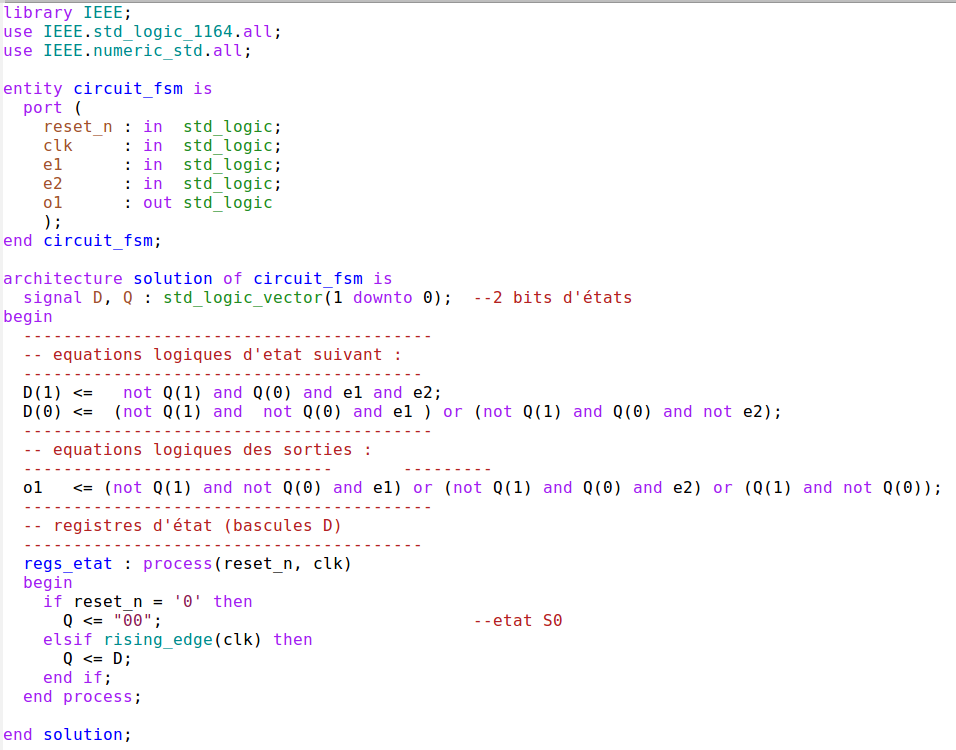
\includegraphics[scale=0.25]{./images/vhdl_1.png}
        %\caption{Vending machine et son environnement}
      \end{figure}
    \end{column}
  \end{columns}
\end{frame}


\begin{frame}{Netlist : après synthèse}
  \begin{columns}
    \begin{column}{0.45\textwidth}
      \begin{figure}[h]
        \centering
        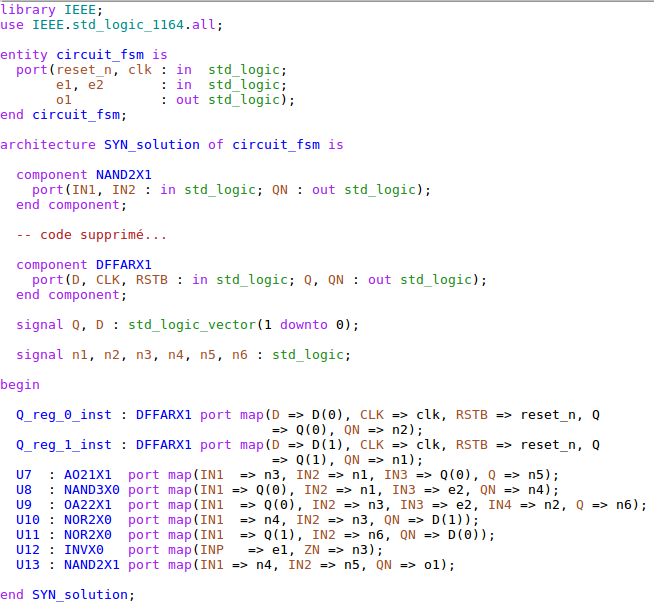
\includegraphics[scale=0.3]{./images/netlist.png}
      \end{figure}
    \end{column}
    \begin{column}{0.55\textwidth}
      \begin{figure}[h]
        \centering
        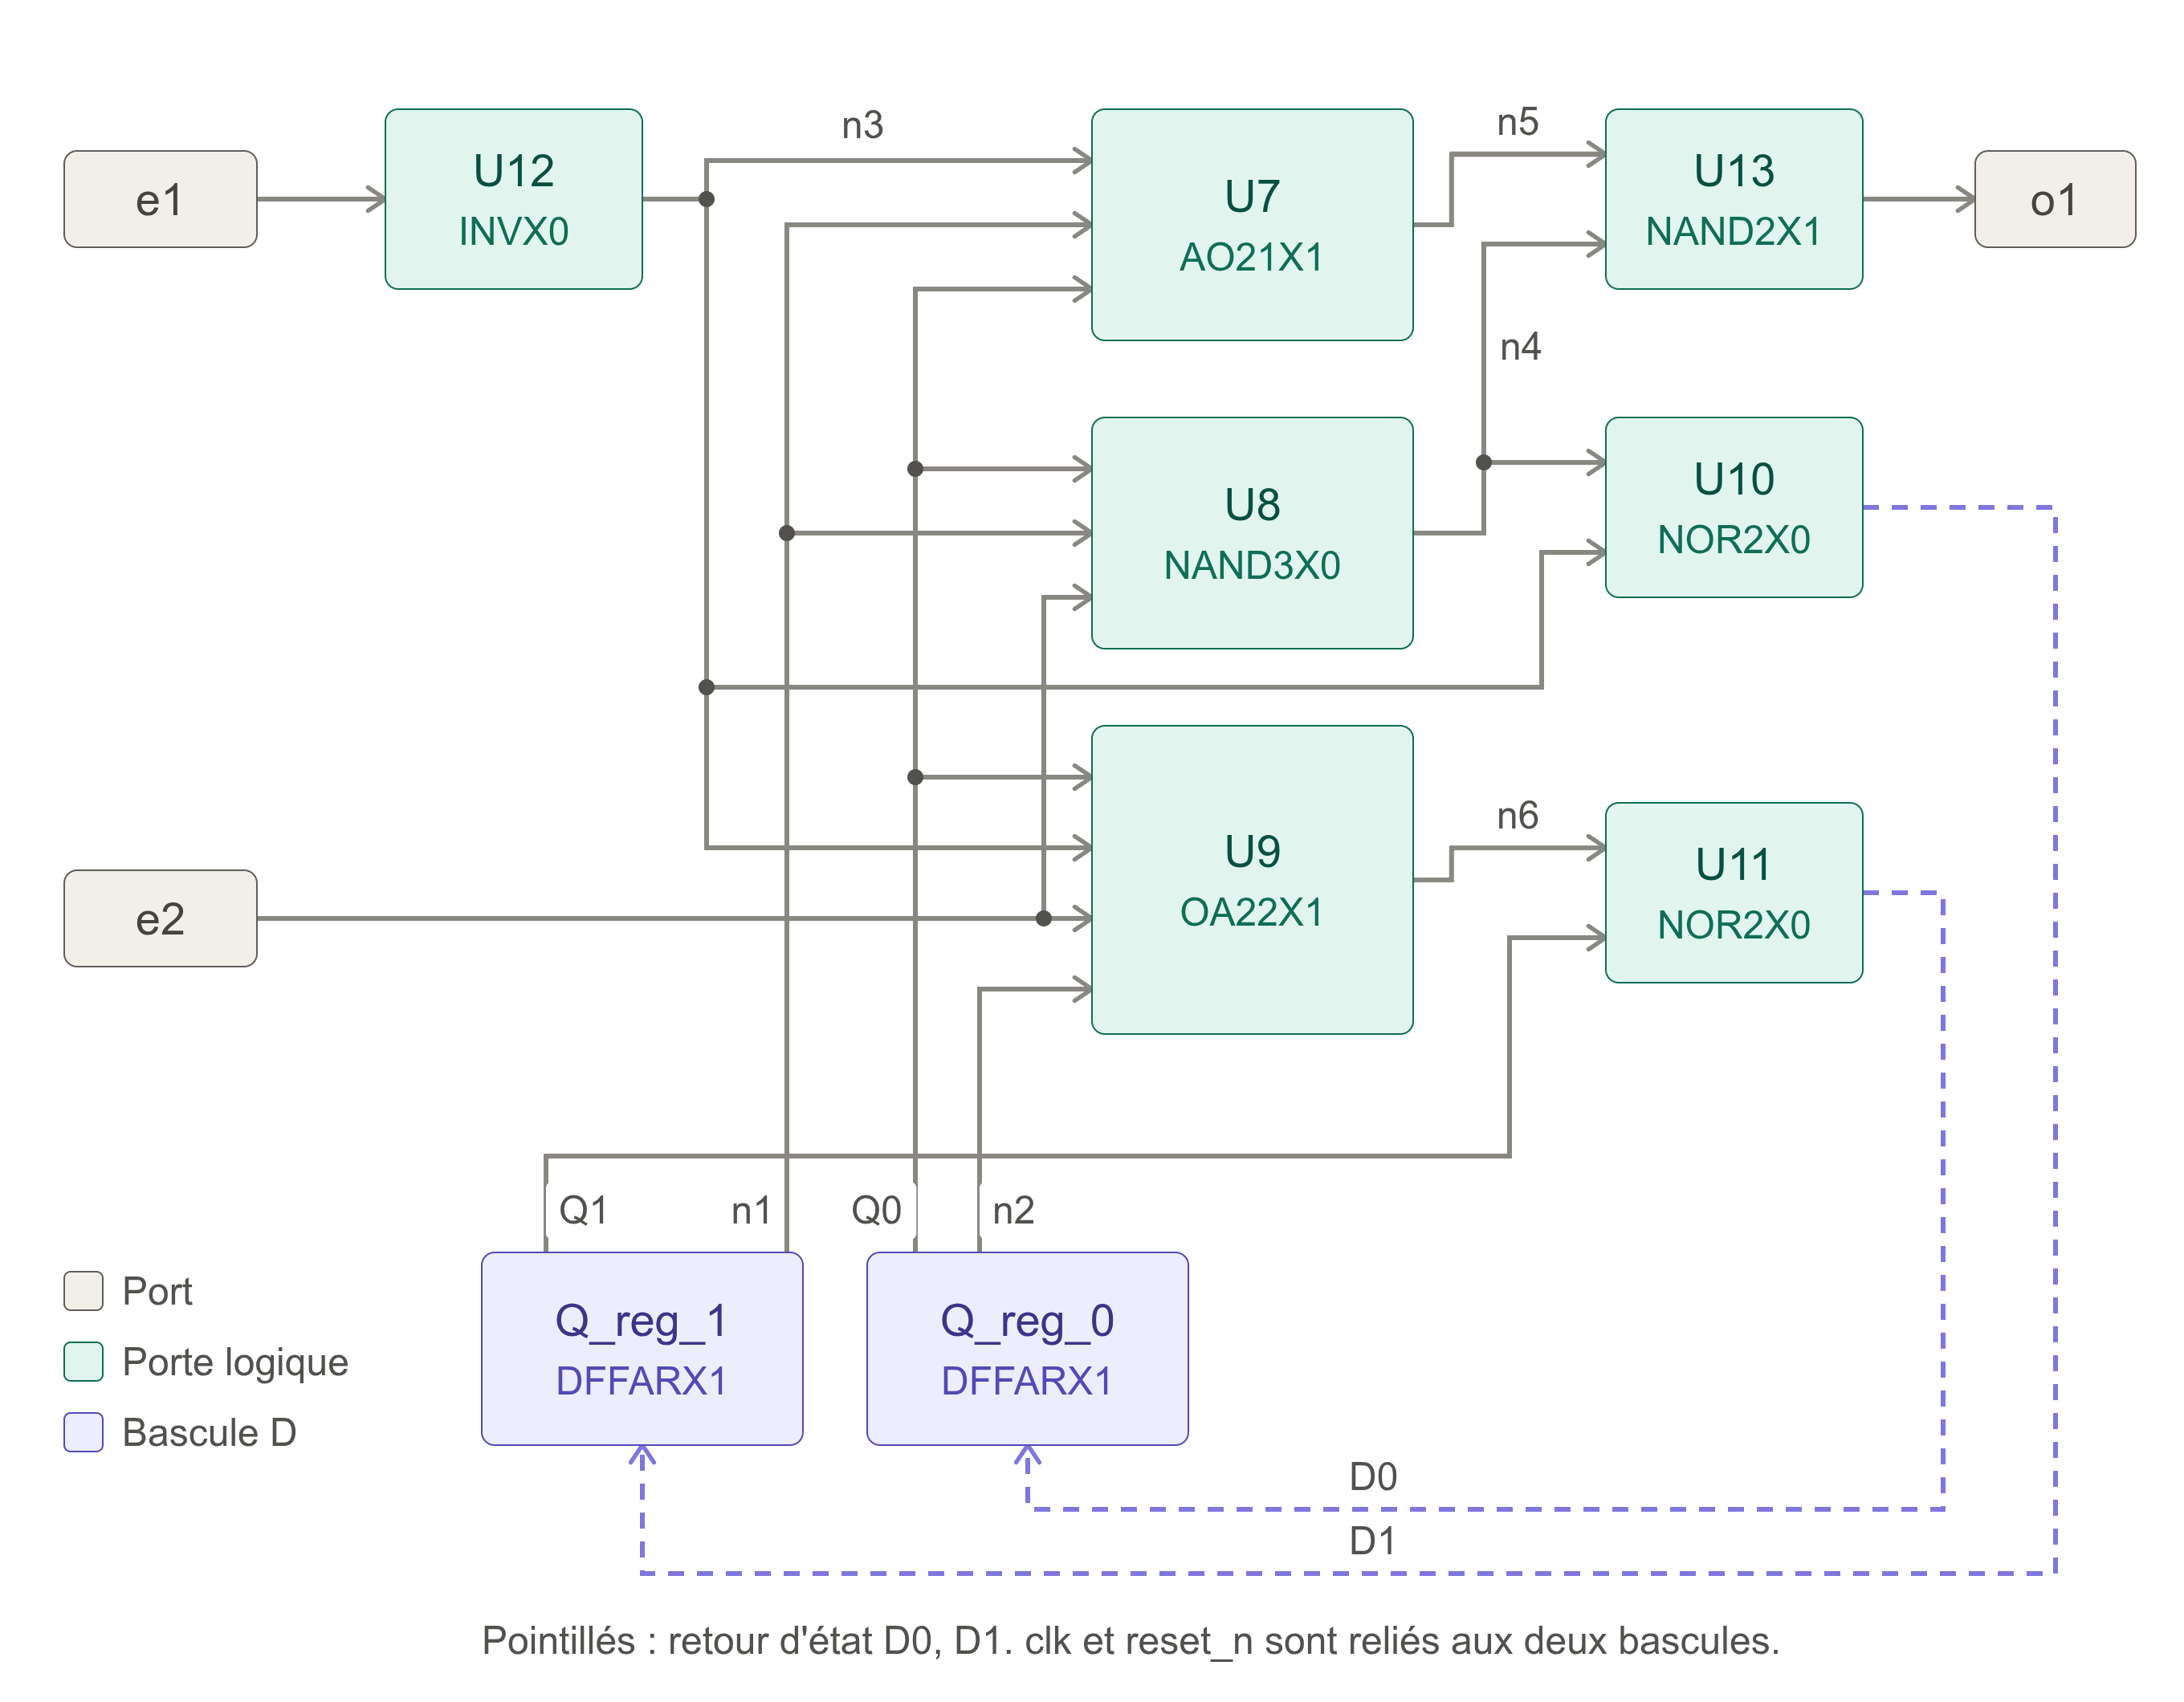
\includegraphics[scale=0.09]{./images/netlist_circuit_fsm_graphe.png}
      \end{figure}
    \end{column}
  \end{columns}
\end{frame}


\begin{frame}{Notion d'entité}
\begin{columns}
  \begin{column}{0.4\textwidth}
    L'\textbf{entity} est la \textbf{vue extérieure} d'un composant.
    \begin{itemize}
      \item Nom du composant
      \item Liste de ports :
      \begin{itemize}
        \item Entrées : \boxed{nom : \textbf{in } type;}
        \item Sorties : \boxed{nom : \textbf{out } type;}
        \item Il est possible de déclarer plusieurs ports comme ceci : \boxed{n1,n2,n3 : \textbf{out } type;}
      \end{itemize}
    \end{itemize}
  \end{column}
  \begin{column}{0.6\textwidth}
    \begin{center}
      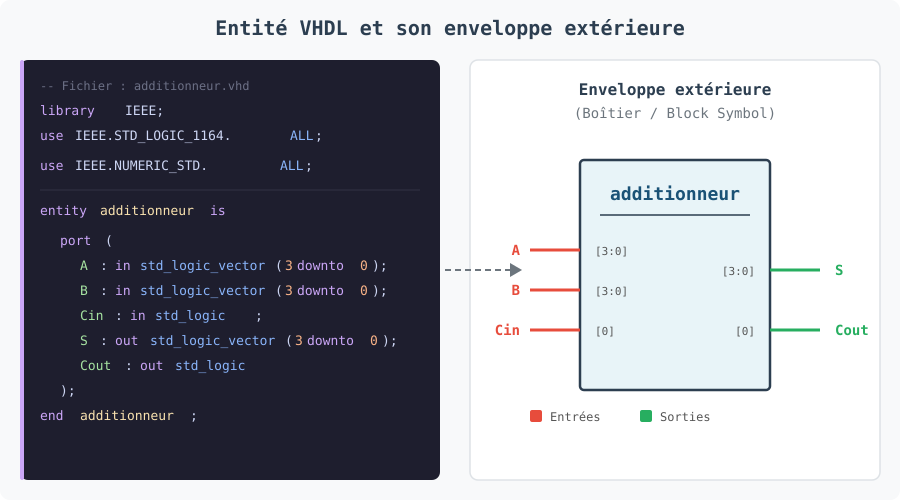
\includegraphics[scale=0.4]{./images/vhdl_entity.png}
    \end{center}
  \end{column}
\end{columns}
\end{frame}

\begin{frame}{Notion d'architecture}
  \begin{columns}

    \begin{column}{0.5\textwidth}
      \begin{alertblock}{Architecture}
        \begin{itemize}
          \item L'architecture : la vue \textbf{interne} d'un composant.
          \item Partie déclaration suivie d'un corps de l'architecture.
          \item Le corps contient des \textbf{éléments qui fonctionnent en parallèle} !
          \begin{itemize}
            \item L'ordre dans lesquels ils sont écrits est indifférent !
            \item On parle plutôt de \textbf{concurrence} (en simulation ces éléments partagent le processeur qui simule...)
          \end{itemize}
        \end{itemize}
      \end{alertblock}
    \end{column}

    \begin{column}{0.5\textwidth}
      \textbf{Eléments concurrents}
      \begin{itemize}
        \item \textbf{Assignations de signaux} : comme des équations.
        \begin{itemize}
          \item les assignations peuvent être conditionnelles ou non.
        \end{itemize}
        \item \textbf{Instanciations de composants} : assemblage hiérarchique.
        \item \textbf{Processus} : codes séquentiels isolés les uns des autres, communicants par \textit{signaux}.
      \end{itemize}
      Nous allons les passer en revue ici.
    \end{column}
  \end{columns}
\end{frame}

\begin{frame}{Architecture : notion d'\textbf{assignations concurrentes}}
  \begin{figure}[h]
    \centering
    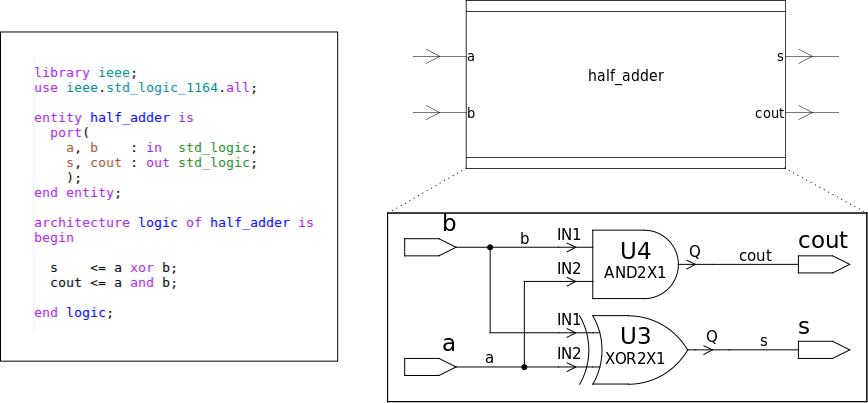
\includegraphics[scale=0.35]{./images/assignations_concurrentes.png}
  \end{figure}
\end{frame}

\begin{frame}{Architecture : notion d'\textbf{instanciation de composants}}
  \begin{figure}[h]
    \centering
    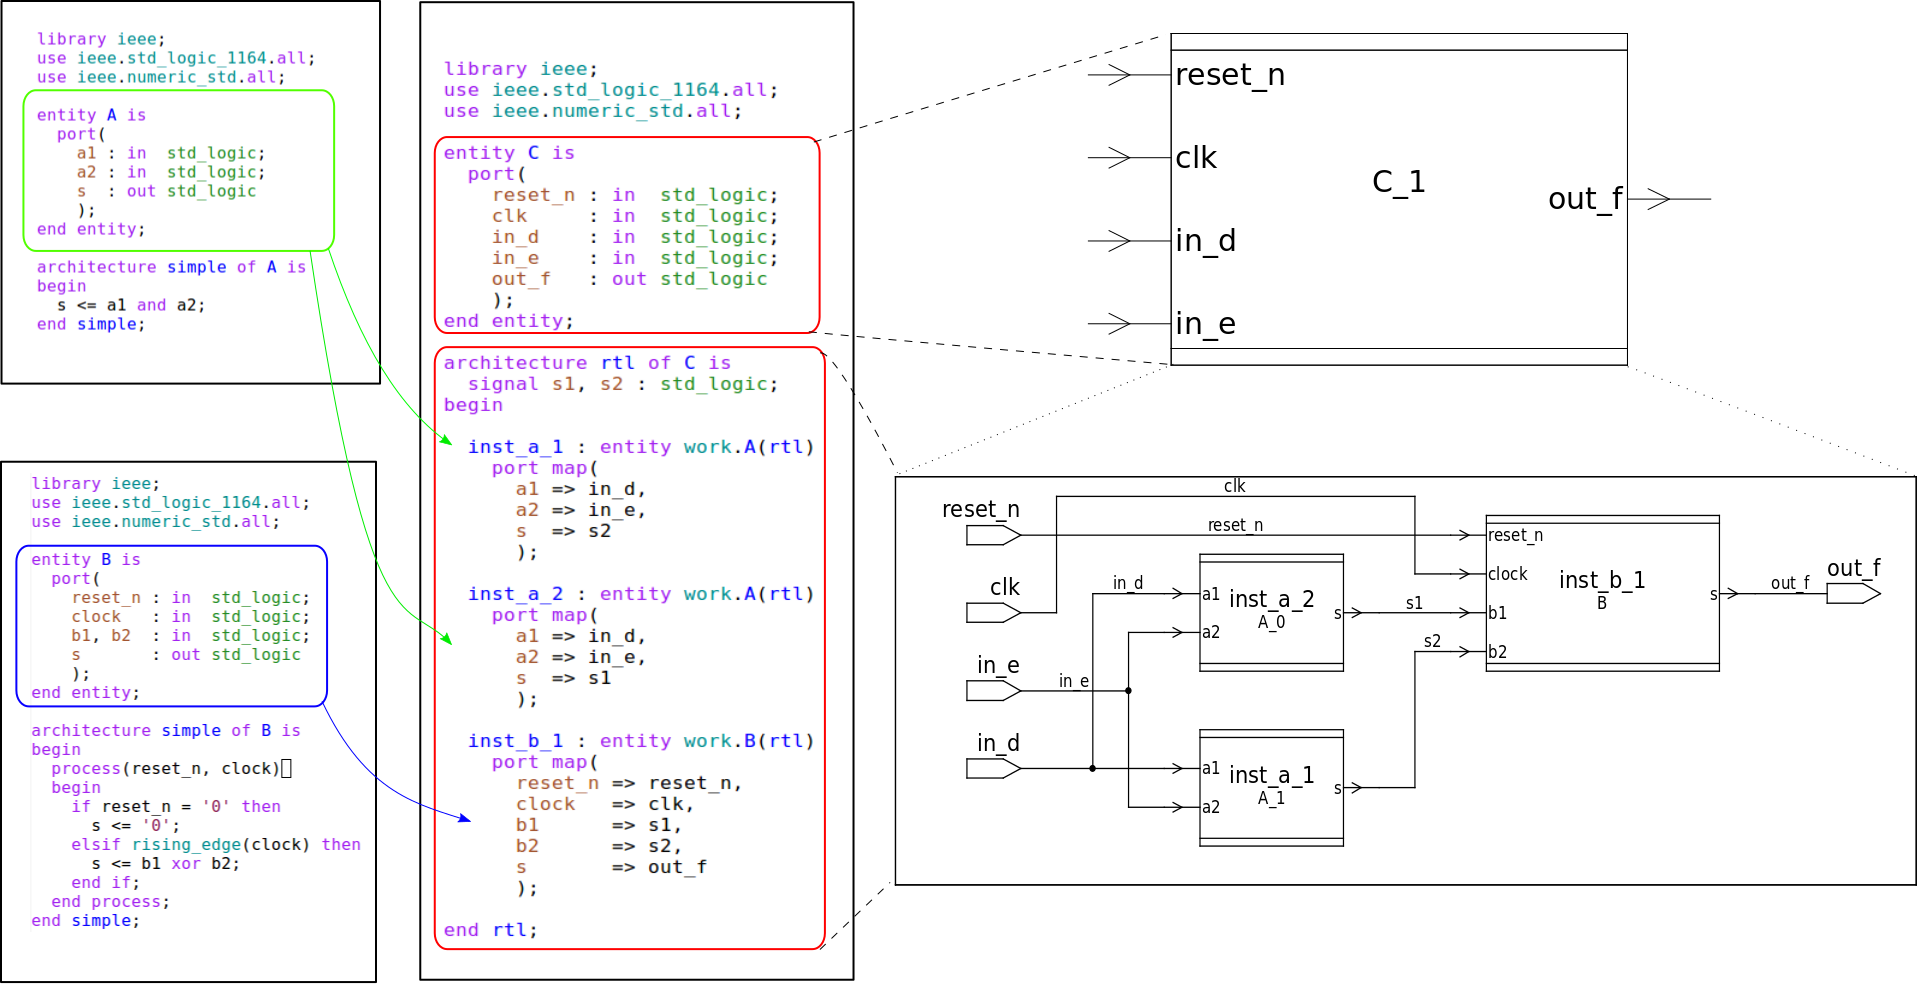
\includegraphics[scale=0.17]{./images/instanciation.png}
  \end{figure}
\end{frame}

\begin{frame}{Architecture : notion de \textbf{processus concurrents}}
  \begin{columns}
    \begin{column}{0.5\textwidth}
      \begin{itemize}
        \item Un processus est un petit programme séquentiel.
        \item Les processus fonctionnent en parallèle (concurrence).
        \item Ils communiquent par signaux.
        \item Une \textbf{liste de sensibilité} explicite permet au simulateur de savoir quand  il doit
        ré-évaluer le processus.
        \begin{itemize}
          \item observation permanente des changements de valeurs impactant le processus
        \end{itemize}
        \item Du point de vue du simulateur, les processus s'exécutent jusqu'à rencontrer un éventuel \textbf{wait}. Sinon, ils rendent la main, avant de se ré-executer.
        \item Du point de vue de la synthèse, les processus nous permettront notamment de décrire les bascules D.
      \end{itemize}
    \end{column}
    \begin{column}{0.5\textwidth}
      \begin{center}
        \includegraphics[scale=0.65]{./images/vhdl_processus.jpeg}
      \end{center}
    \end{column}
  \end{columns}
\end{frame}

\begin{frame}{Processus concurrents : exemple}
  \begin{figure}[h]
    \centering
    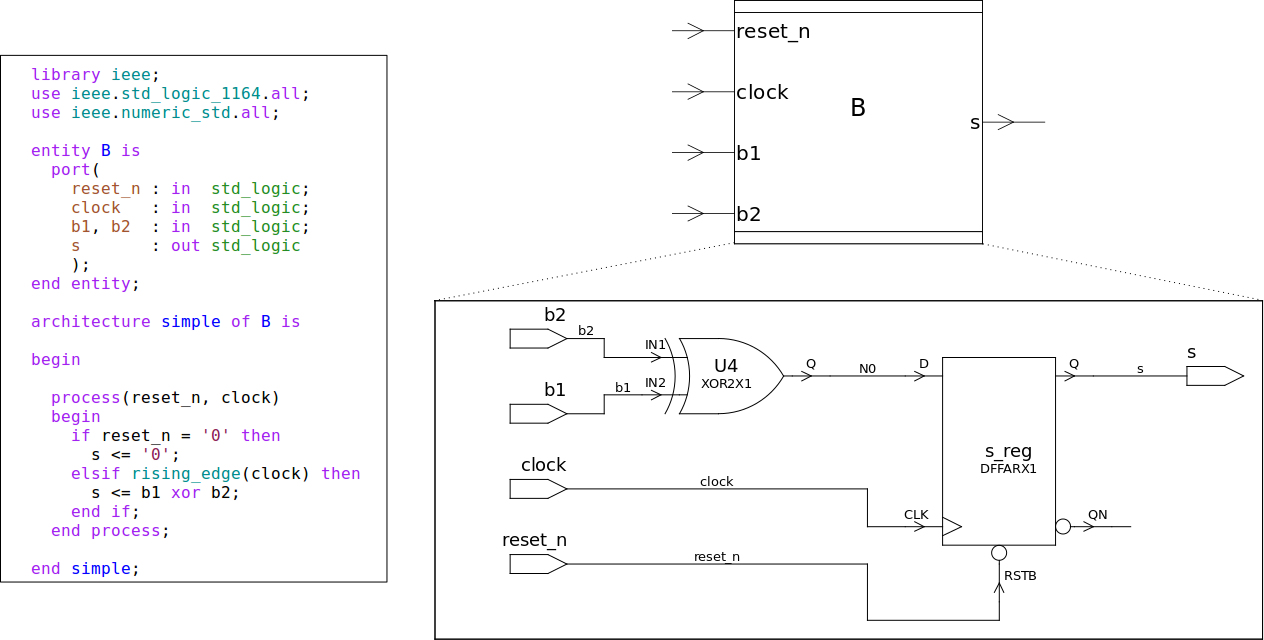
\includegraphics[scale=0.25]{./images/processus_sequentiel.png}
  \end{figure}
\end{frame}

\begin{frame}{Types en VHDL}
  On dispose de type de base, inclus dans le langage (bit par exemple), mais on repose
  plutôt sur des librairies complémentaires :
  \begin{itemize}
    \item \textbf{std\_logic\_1164} : type std\_logic, std\_logic\_vector
    \item \textbf{std\_logic} : '1','0', mais aussi 'Z','X','U','L','H'
    \begin{itemize}
      \item '0','1' : logique booléenne traditionnelle
      \item 'U' : signal 'Undefined' (non connecté)
      \item 'X' : signal en conflit. Plusieurs connexions cherchent à affecter le signal.
      \item 'Z' : haute impédance.
      \item 'L','H' : signal à peu près à '0' et '1' (peu usités)
    \end{itemize}
    \item \textbf{numeric\_std} : arithmétique traditionnelle.
    \item etc.
  \end{itemize}
  Il est possible de créer ses propres types.
  \begin{itemize}
    \item types \textbf{structurés} : \texttt{record}
    \item types \textbf{énumérés}   : \texttt{enum}
    \item types \textbf{tableaux}   : \texttt{array..of..}
  \end{itemize}
\end{frame}

\begin{frame}{Décrire des automates : en équations}
  \begin{figure}[h]
    \centering
    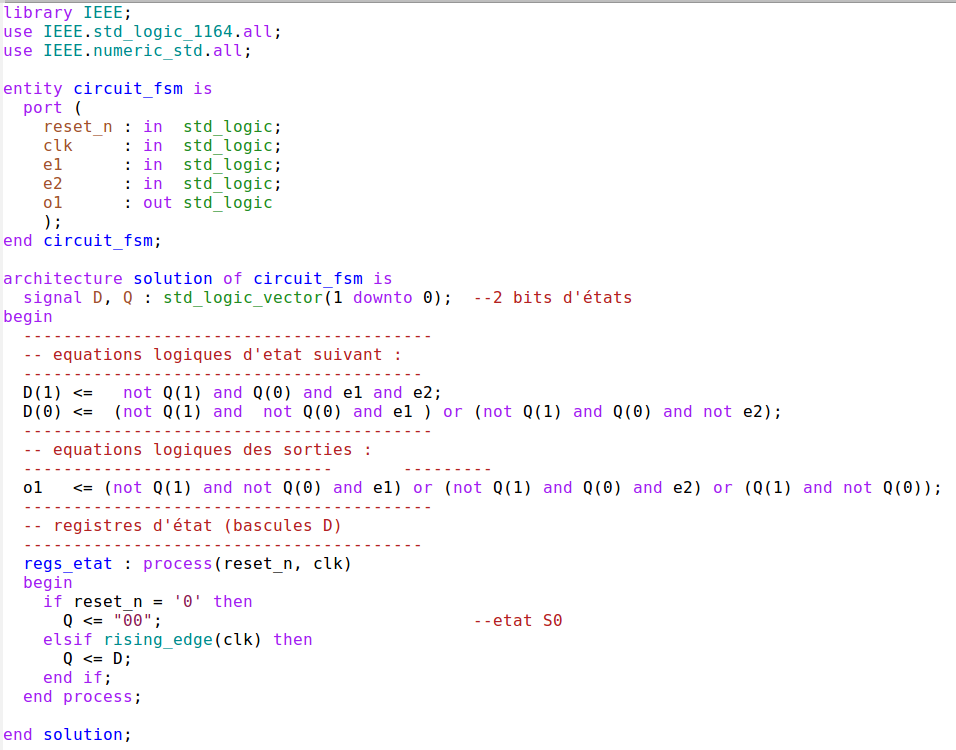
\includegraphics[scale=0.28]{./images/vhdl_1.png}
  \end{figure}
\end{frame}

\begin{frame}{Décrire des automates : en RTL}
  \begin{figure}[h]
    \centering
    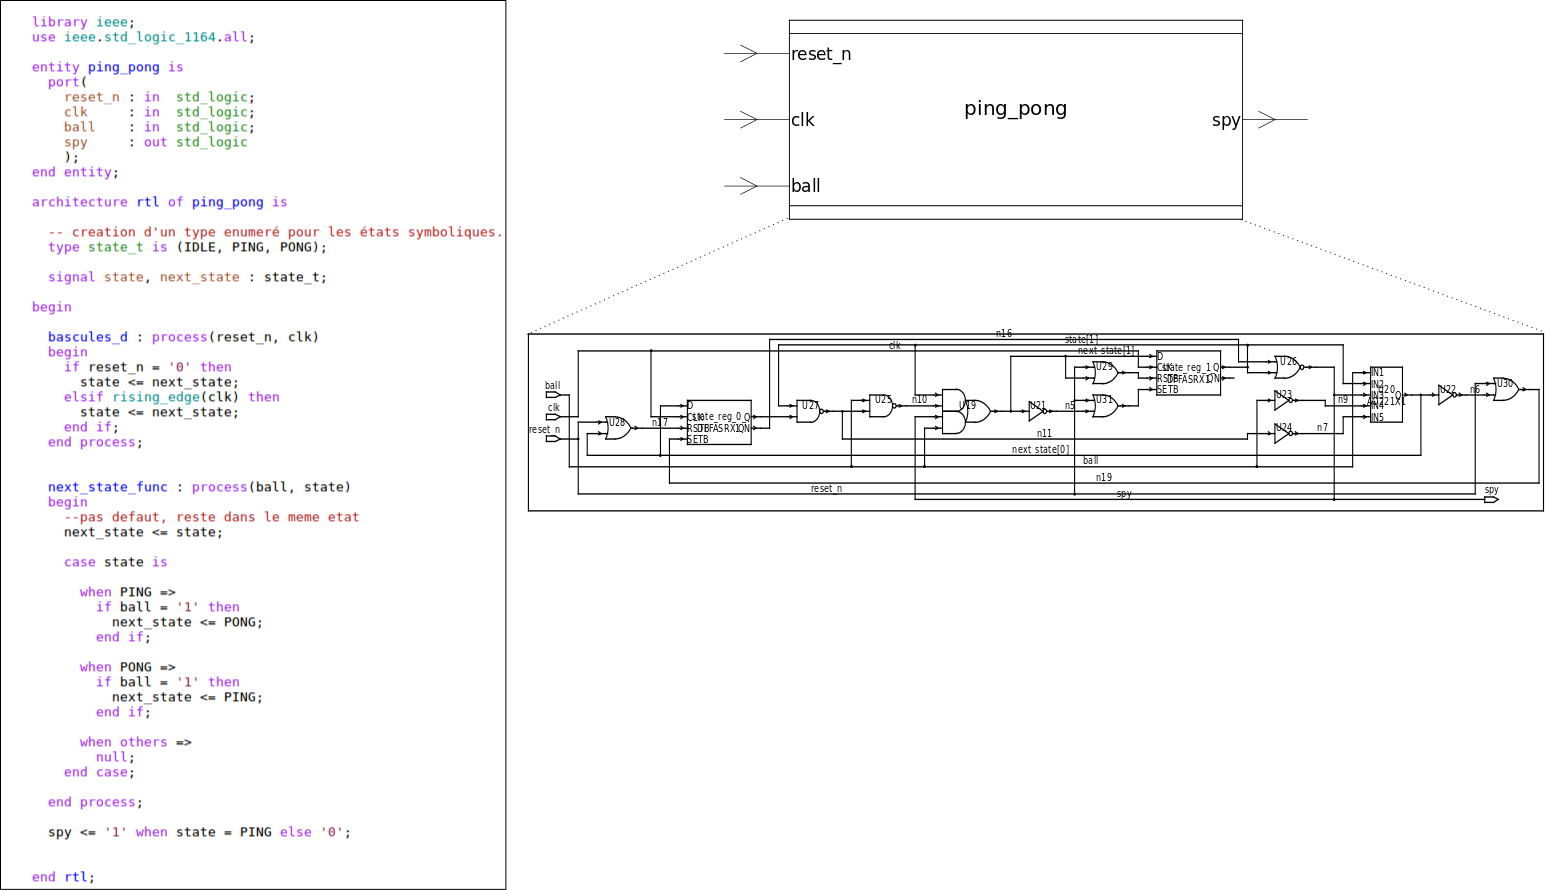
\includegraphics[scale=0.21]{./images/ping_pong_rtl.png}
  \end{figure}
  %\begin{alertblock}{Synthèse RTL}
    Le synthétiseur est capable d'\textit{inférer} les équations logiques de ce style de descriptions RTL.
  %\end{alertblock}
\end{frame}

\begin{frame}{Décrire des automates : en RTL}
  \begin{itemize}
    \item Les états sont représentés par un \textbf{type énumeré}.
    \item Deux signaux \textbf{state,next\_state} codent l'état courant et l'état futur.
    \item Un processus combinatoire permet d'expliciter le signal {\it next\_state}, à l'aide
    de différents {\it cas} présents dans le \textbf{case...when} du langage.
    \item Un processus séquentiel réalise l'échantillonnage et l'affectation de {\it next\_state} dans {\it state}
  \end{itemize}
\end{frame}

\begin{frame}{Décrire des automates : en RTL}
  \begin{itemize}
    \item A ce stade, le synthétiseur a suffisamment d'informations, pour \textbf{inférer} les équations logiques.
    \item Il a au préalable choisi un encodage de l'état. Cet encodage peut être forcé dans VHDL par des attributs ou guidés par des scripts.
    \item Le synthétiseur est capable d'explorer plusieurs solutions, notamment en fonction de l'encodage.
    \item Les sorties peuvent être encodées dans un troisème processus, mais généralement on les retrouvent dans le même processus que le calcul
    de l'état suivant.
  \end{itemize}
\end{frame}

\begin{frame}{Bancs de tests ou \textit{testbenchs}}

  \begin{columns}
    \begin{column}{0.55\textwidth}
      Les {\it testbenchs} représentent un \textbf{laboratoire virtuel} :
      \begin{itemize}
        \item le circuit à tester (DUT)
        \item des générateurs de signaux : horloge, reset, flux de données complexes.
        \item des instruments d'observations : loggers, comparateurs, etc
        \item la simulation elle-même fournit un oscilloscope, capable d'observer:
        \begin{itemize}
          \item la totalité des signaux
          \item sur une durée limitée par la seule mémoire de l'ordinateur
        \end{itemize}
      \end{itemize}

      A noter :
      \begin{itemize}
        \item seul un testbench est simulable.
        \item les bancs de test sont également décrits par un couple entité-architecture.
        \item \texttt{entity} sans port : laboratoire portes closes !
      \end{itemize}
    \end{column}
    \begin{column}{0.45\textwidth}
      \begin{center}
          \centering
          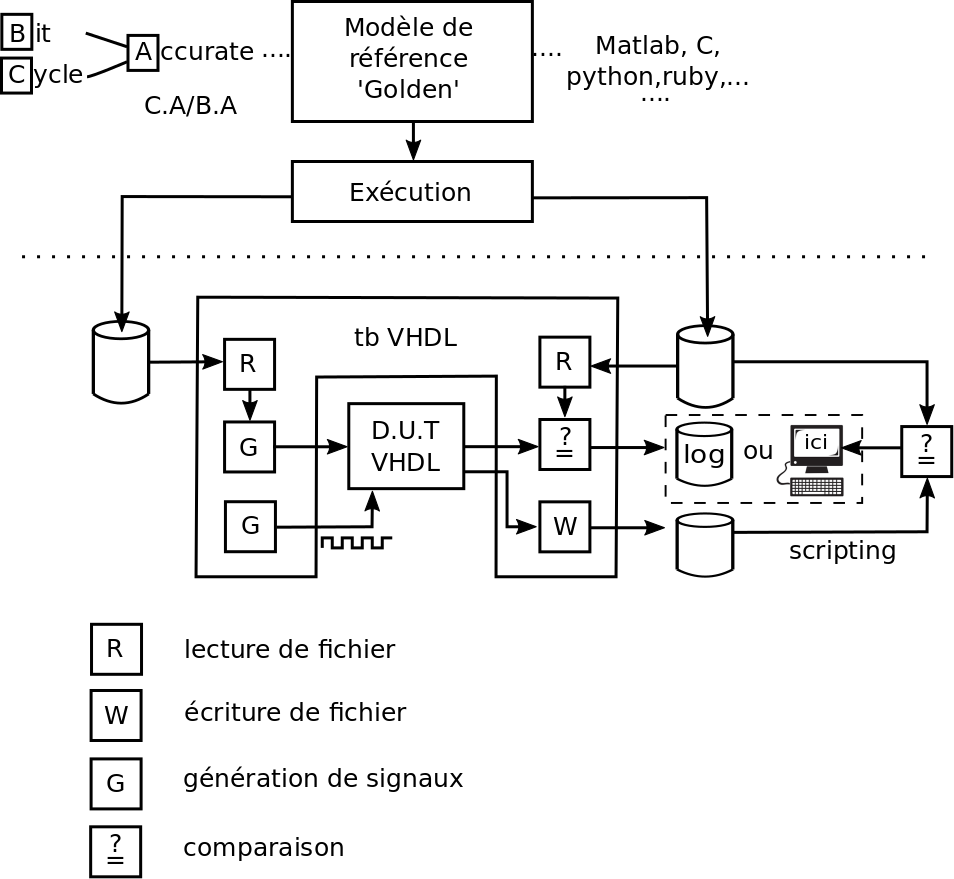
\includegraphics[scale=0.2]{./images/flot_testbench.png}
      \end{center}
    \end{column}
  \end{columns}
\end{frame}

\begin{frame}{Bancs de tests}
  \begin{itemize}
    \item Les {\it testbenchs} VHDL sont le seul moyen de tester si un circuit fonctionne correctement : un circuit seul ne fonctionne pas.
    \item Les {\it testbenchs} peuvent être de différentes natures et représentent l'essentiel du travail de concepteur.
    \begin{itemize}
      \item Testbenchs qui stimulent seulement les entrées, à partir de stimuli internes.
      \item Testbenchs qui stimulent seulement les entrées, à partir de stimuli externes (matlab, python, ruby, c, c++).
      \item Testbenchs qui vérifient les sorties, en calculant en interne les sorties attendues.
      \item Testbenchs qui vérifient les sorties, en les comparant à des valeurs calculées par un modèle externe : le \textbf{golden model}.
      \item Testbenchs qui "randomisent" la vérification, afin d'assurer une \textbf{couverture de code}.
    \end{itemize}

  \end{itemize}
\end{frame}

\begin{frame}{Banc de test VHDL : FSM \texttt{metro-boulot-dodo}}
  \begin{center}
  \begin{minipage}[t]{15cm}
   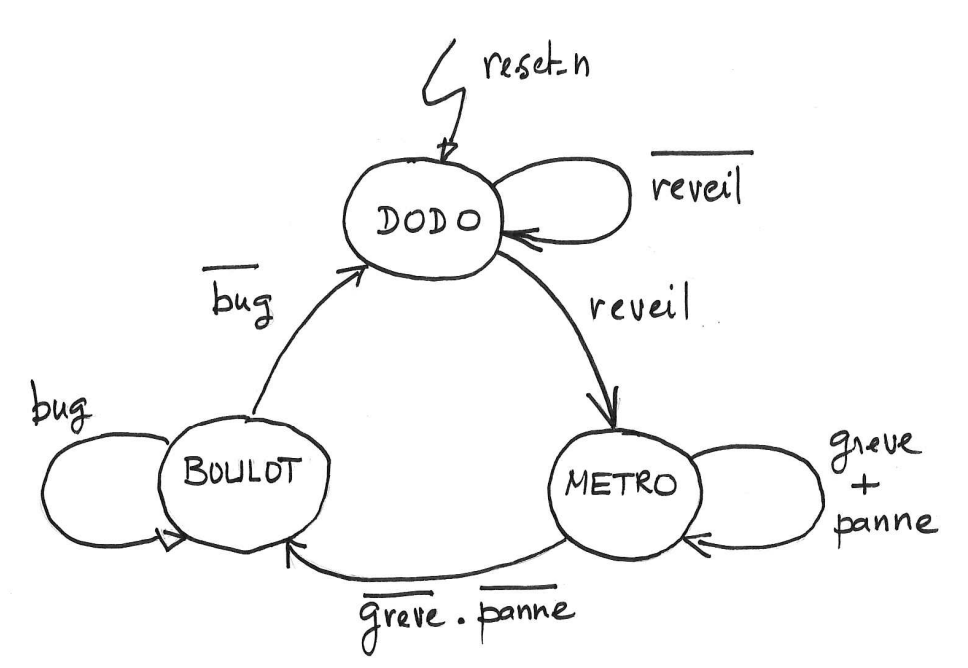
\includegraphics[width=10cm]{./images/iloveparis.png}
  \end{minipage}
  \end{center}
\end{frame}

\begin{frame}{Banc de test VHDL : exemple}
  \begin{center}
   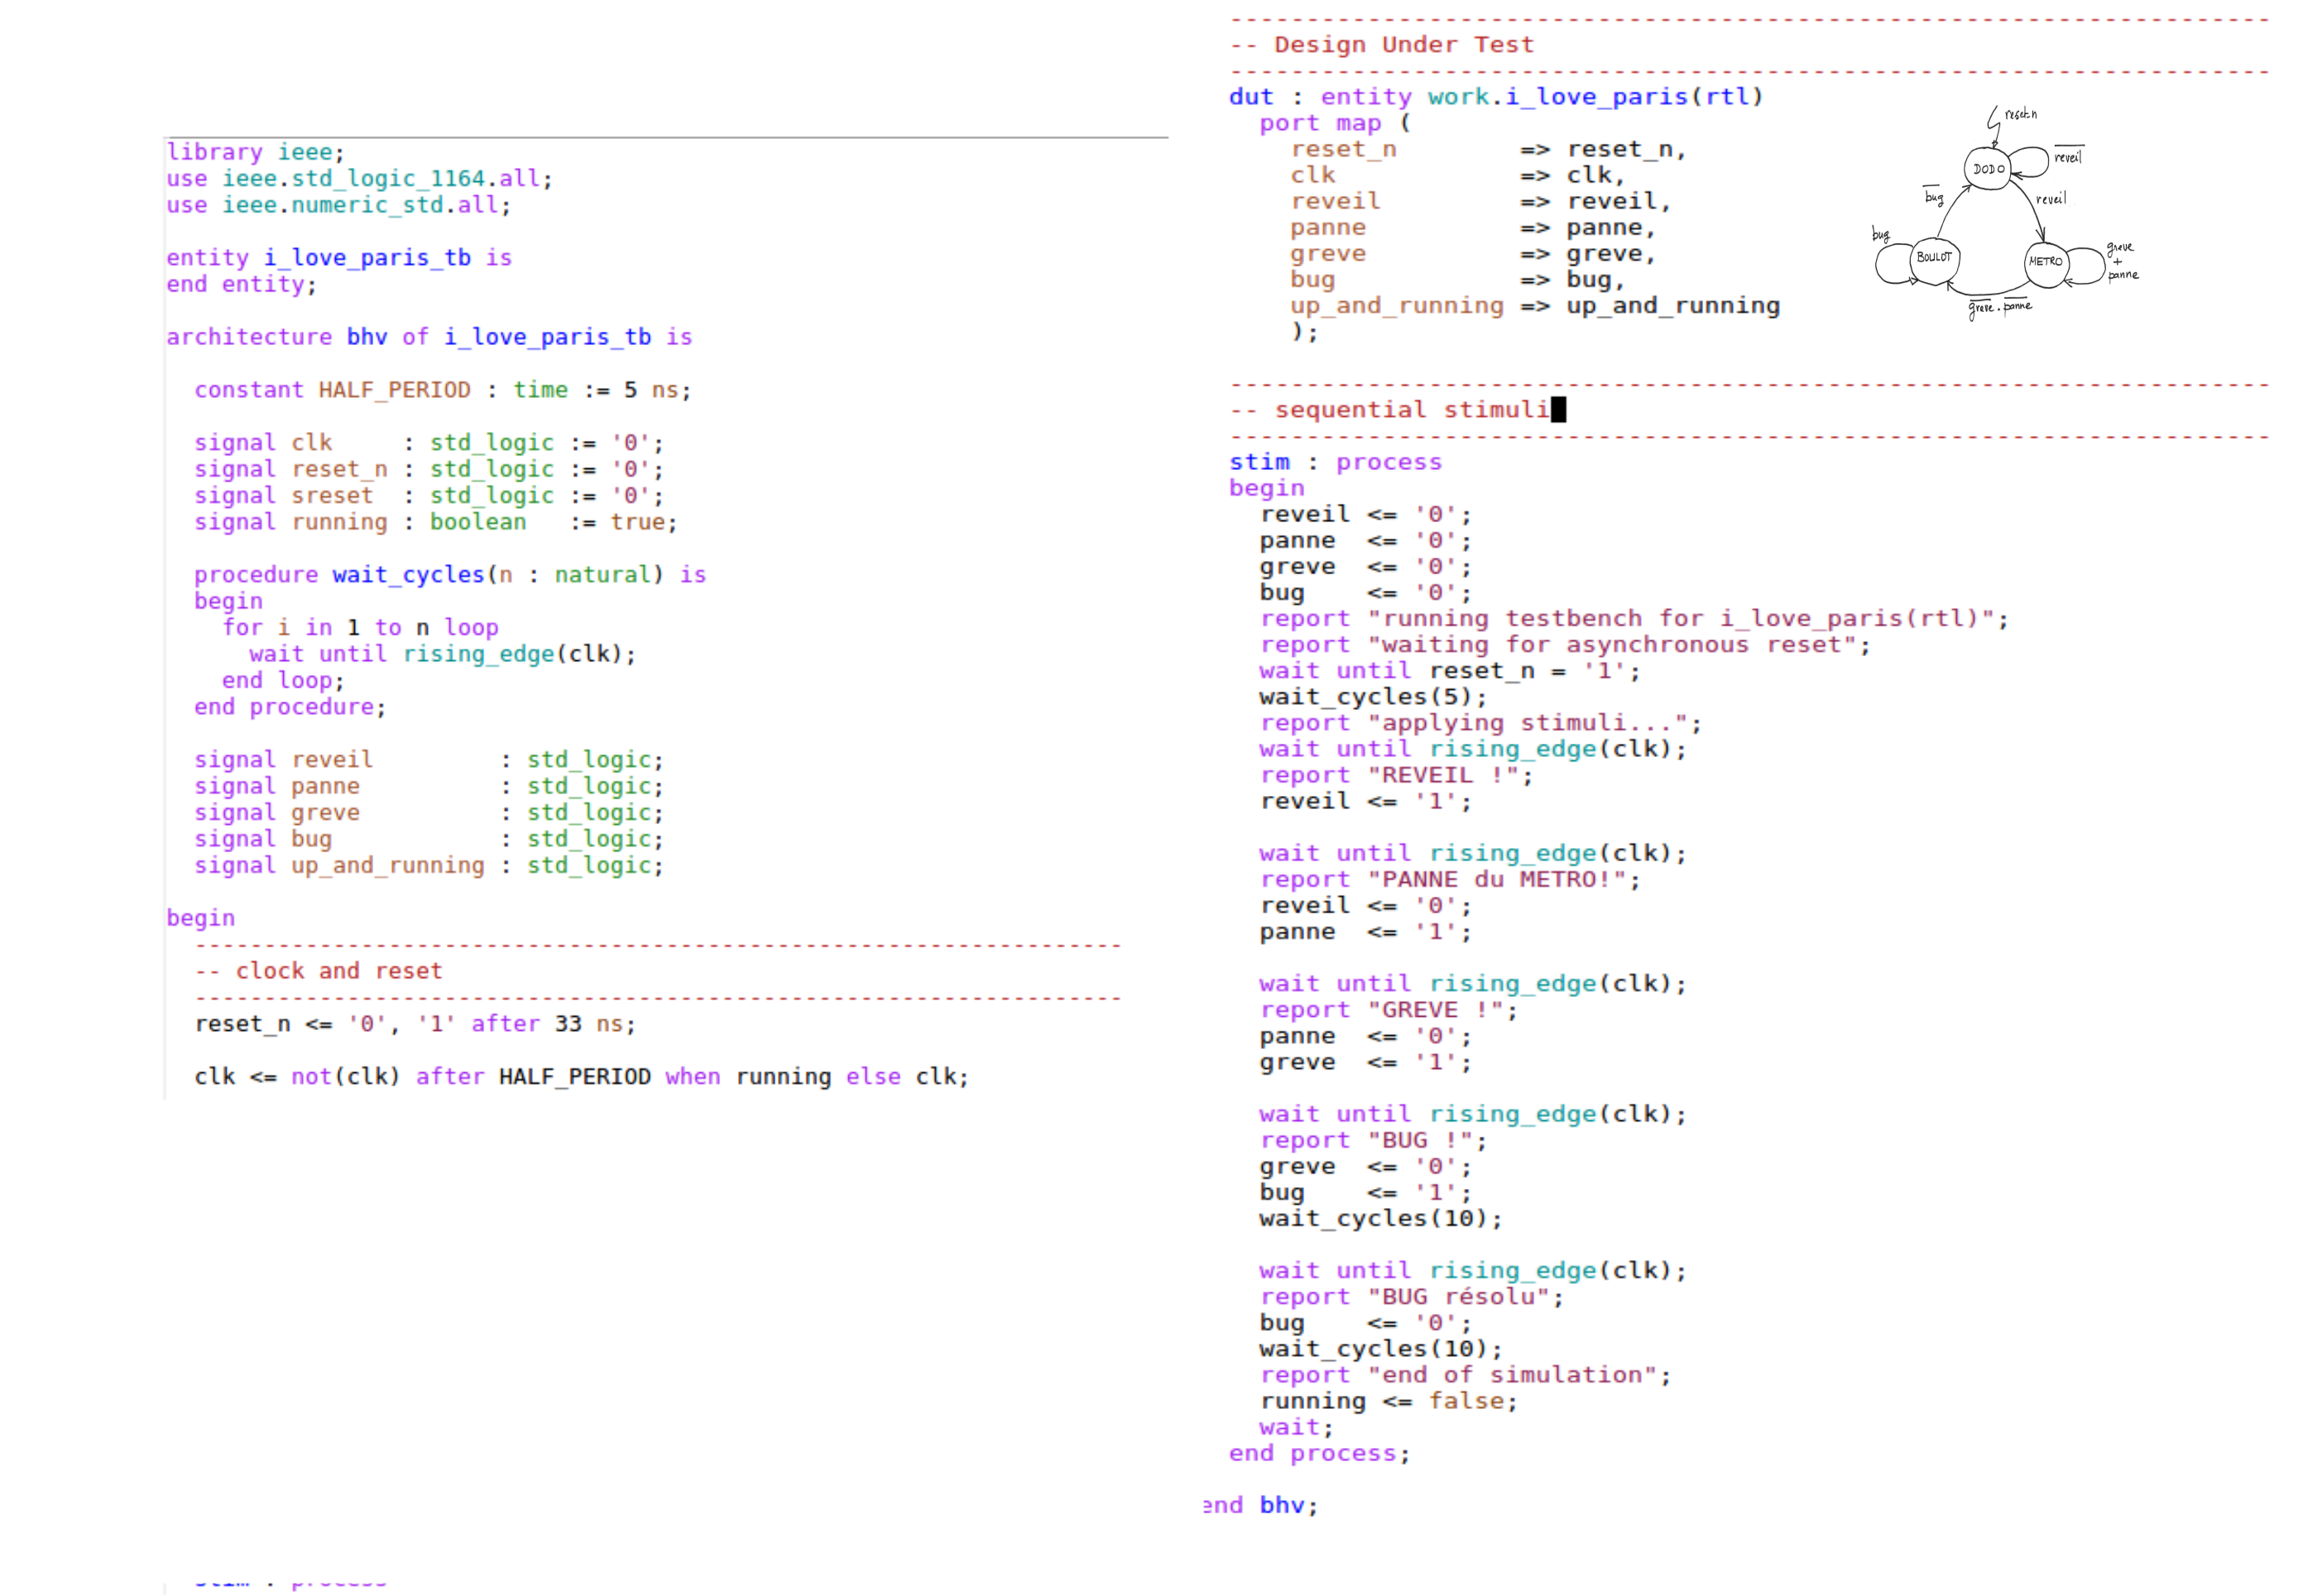
\includegraphics[scale=0.12]{./images/tb_000.png}
  \end{center}
\end{frame}

\begin{frame}{Banc de test VHDL : exemple}
  \begin{center}
   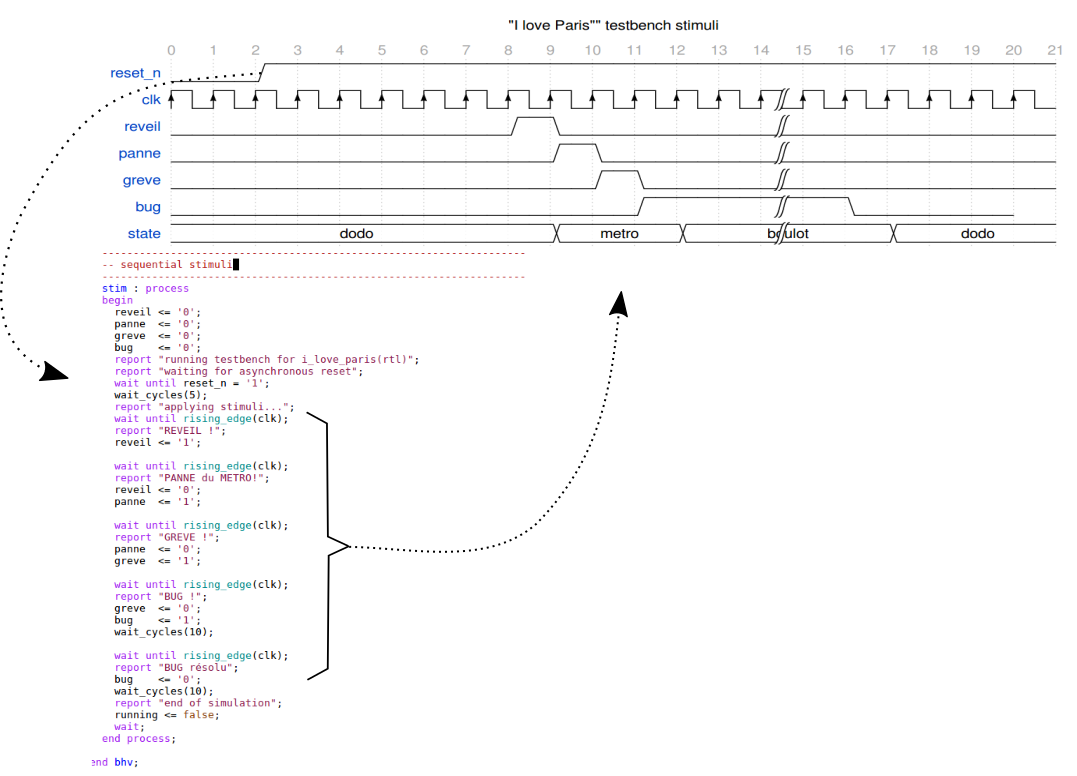
\includegraphics[scale=0.28]{./images/wave_drom.png}
  \end{center}
\end{frame}

\begin{frame}{Pour la petite histoire...}
  Les {\it timing diagrams} ont été crées avec une syntaxe textuelle ! Le compilateur
  transforme ces {\it timing diagrams} en graphique SVG dans html5.
  \begin{center}
  \begin{minipage}[t]{19cm}
   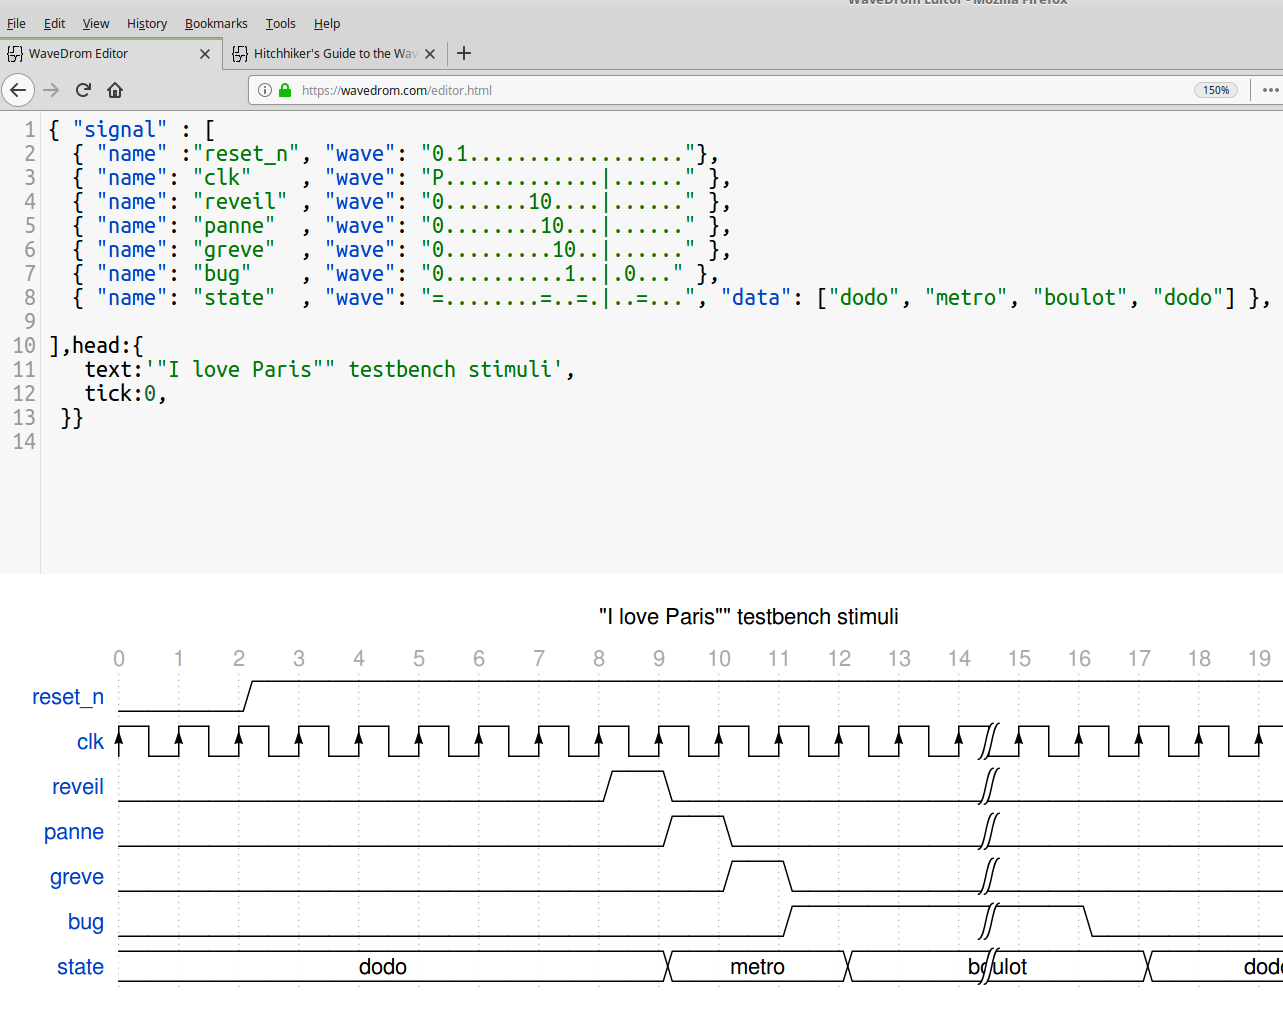
\includegraphics[scale=0.17]{./images/wave_drom_ex.png}
  \end{minipage}
  \end{center}
\end{frame}

\begin{frame}{Banc de test VHDL : exemple}
  Chronogrammes issus de la chaîne de compilation-simulation-visualisation autour de GHDL+Gtkwave.
  \begin{center}
  \begin{minipage}[t]{19cm}
   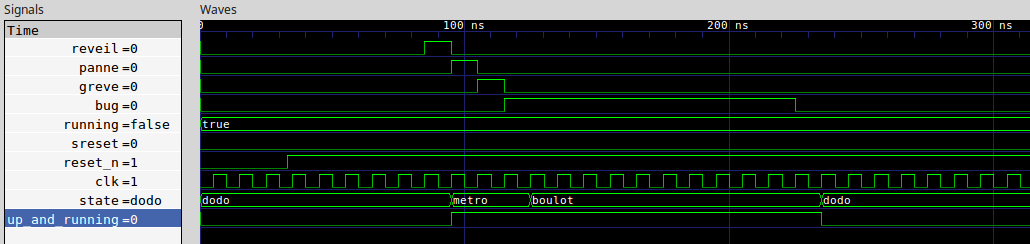
\includegraphics[scale=0.32]{./images/metro_boulot_dodo_chrono.png}
  \end{minipage}
  \end{center}
\end{frame}

\begin{frame}{Simulation avec GHDL ou NVC}
  \begin{columns}
    \begin{column}{0.5\textwidth}
      \texttt{GHDL} est un simulateur et synthétiseur open source développé par un français : Tristan Gingold.
      \begin{itemize}
        \item Il est open source. Développé en ADA.
        \item Il supporte les évolutions récentes du langage.
        \item Il est scrupuleux sur le respect de la norme.
        \item On peut le coupler à \texttt{gtkwave} pour l'examen des signaux.
        \item Ce n'est pas le simulateur le plus utilisé au Monde : il s'agit de Modelsim.
      \end{itemize}
      \texttt{NVC} est un autre simulateur (pas de synthèse) open source développé par un brittanique : Nick Gasson.
    \end{column}
    \begin{column}{0.5\textwidth}
      \begin{center}
        \begin{figure}
          \includegraphics[scale=0.2]{./images/Tristan_Gingold.jpg}
          \caption{Tristan Gingold, ingénieur de Recherche au \texttt{C.E.R.N}, Génève (Telecom Paris 96, DEA Microélectronique (Paris 6) 98.)}
        \end{figure}
      \end{center}
    \end{column}
  \end{columns}
\end{frame}

\begin{frame}{Simulation avec GHDL}
  Pour simuler un testbench, il faut passer par 3 phases :
  \begin{itemize}
    \item \textbf{A}nalyse : \textbf{ ghdl -a circuit.vhd}
    \item ...
    \item \textbf{A}nalyse : \textbf{ghdl -a circuit\_tb.vhd}
    \item \textbf{E}laboration : \textbf{ghdl -e circuit\_tb} (sans .vhd).
    \begin{itemize}
      \item cette phase réunit les fichiers binaires produits par l'analyse
      \item ...adjoint un {\it runtime} (le coeur du simulateur)
      \item ...et produit un exécutable : le simulateur
    \end{itemize}
    \item \textbf{R}un : \textbf{ghdl -r circuit\_tb --wave=waves.ghw}.
    \begin{itemize}
      \item Le simulateur s'exécute et enregistre les signaux dans le fichier waves.
    \end{itemize}
    \item Un viewer externe est alors utilisé pour visualiser les signaux : \textbf{gtkwave waves.ghw}.
    \item La disposition des signaux est enregistrable dans un fichier spécifique à gtkwave (.sav).
    \item Il faut \textbf{scripter} l'ensemble.
  \end{itemize}
\end{frame}

\begin{frame}{Visualisation avec Gtkwave}
  \textbf{gtkwave wave.ghw chrono.sav}
  Le fichier chrono.sav correspond à la mise en forme des chronogrammes, sauvée dans ce fichier.
  \begin{center}
  \begin{minipage}[t]{8cm}
   \centering
   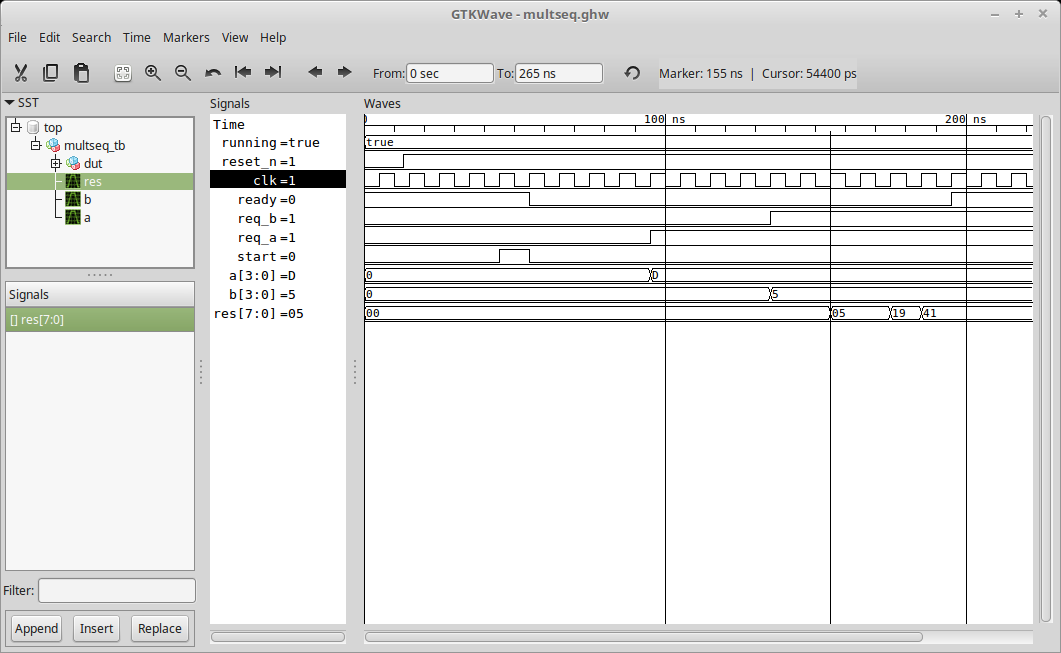
\includegraphics[width=8cm]{./images/gtkwave.png}
  \end{minipage}
  \end{center}
\end{frame}

%========================================================================================
\section{Micro-architectures FSMD}
% %========================================================================================
% 
\begin{frame}{FSMD : architecture contrôleur-chemin de données}
  \begin{alertblock}{FSMD \textit{explicite}}
    \begin{itemize}
      \item Finite State Machine + Datapath : microarchitecture dédiée à un algorithme.
    \end{itemize}
  \end{alertblock}
  \begin{columns}
    \begin{column}{0.5\textwidth}
      \begin{itemize}
        \item \textbf{Décomposition} explicite contrôle-données :
        \begin{itemize}
          \item Rôle de la \textbf{FSM} :
          \begin{itemize}
            \item Observation d'un signal de \textbf{démarrage}.
            \item \textbf{Séquencement} des calculs.
            \item Observation des \textbf{status} au cours des calculs et \textbf{prises de décision}.
            \item Activation des \textbf{contrôles}.
            \item Emission d'un signal de \textbf{terminaison}.
          \end{itemize}
          \item Rôle du \textbf{Datapath} :
          \begin{itemize}
            \item Réception des données externes
            \item Stockage des données internes
            \item Calculs (souvent parallèles)
            \item Production des sorties
          \end{itemize}
        \end{itemize}
        \item Il s'agit d'une structure \textbf{générique}.
      \end{itemize}
    \end{column}
    \begin{column}{0.5\textwidth}
      \begin{center}
        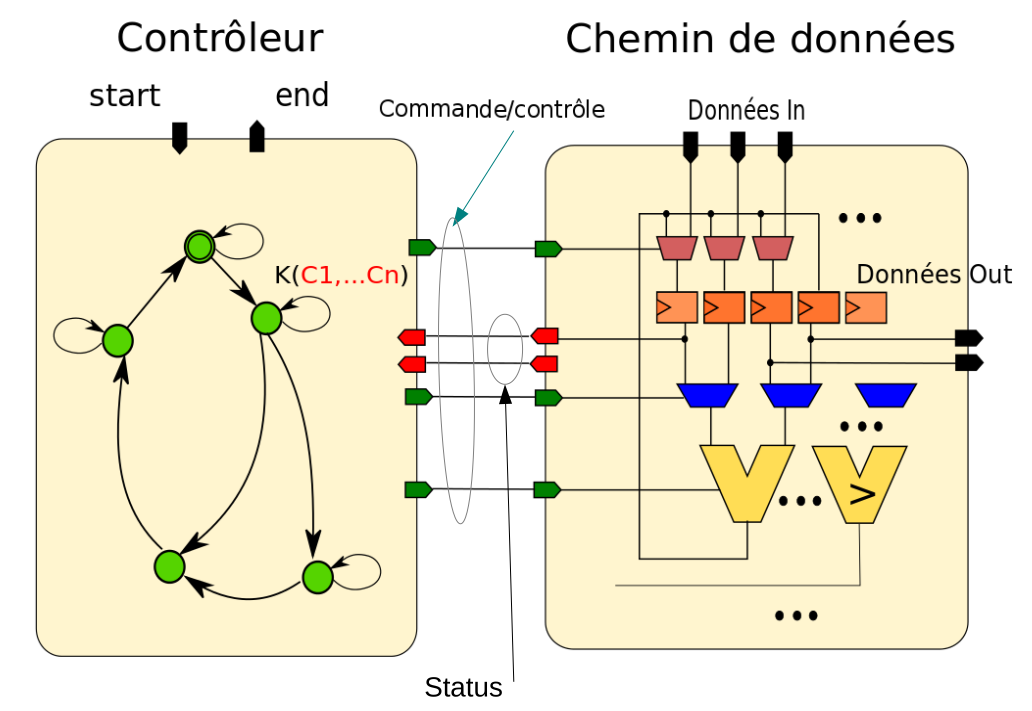
\includegraphics[scale=0.2]{./images/fsmd_0}
      \end{center}
    \end{column}
  \end{columns}
\end{frame}

\begin{frame}{FSMD : généricité du \texttt{datapath}}
  \begin{columns}
    \begin{column}{0.45\textwidth}
      \begin{itemize}
        \item Quatre étages ou \textit{couches} internes :
        \begin{enumerate}
          \item Couche de routage (mux):
          \begin{itemize}
            \item Acheminement des données aux registres
          \end{itemize}
          \item Couche de registres :
          \begin{itemize}
            \item Stockage des variables
          \end{itemize}
          \item Couche de routage (mux):
          \begin{itemize}
            \item Acheminement des données aux opérateurs.
          \end{itemize}
          \item Couche d'opérateurs :
          \begin{itemize}
            \item calculs arithmétiques et logiques.
          \end{itemize}

        \end{enumerate}
      \item Notez les possibilités importantes de \textbf{parallélisme de calculs} simultanés.
      \end{itemize}
    \end{column}
    \begin{column}{0.55\textwidth}
      \begin{center}
        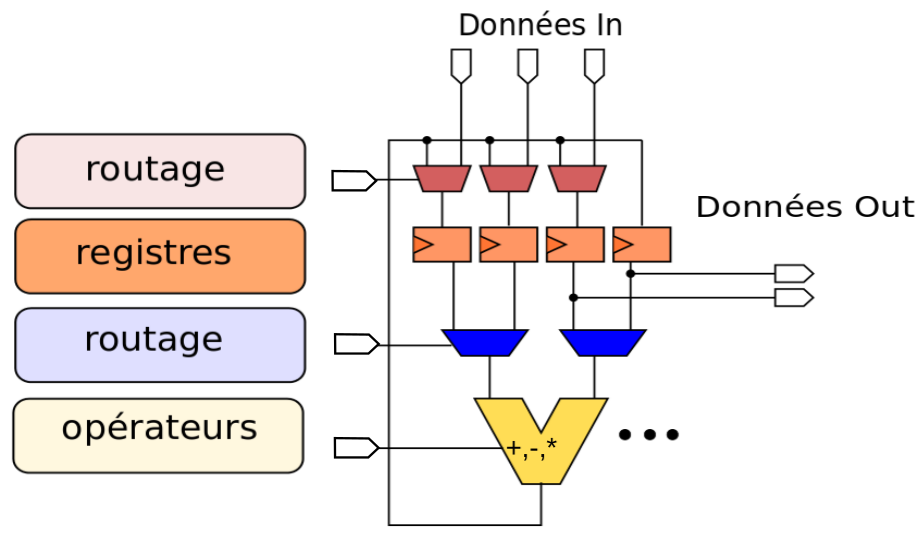
\includegraphics[scale=0.35]{./images/datapath_1}
      \end{center}
    \end{column}
  \end{columns}
\end{frame}

\begin{frame}{Algorithme du PGCD d'Euclide (par soustractions)}
  \textbf{Rappel : } Environ \textbf{300 av. J.-C.}
    \begin{columns}[T]

        % --- COLONNE 1 : L'ALGORITHME ---
        \begin{column}{0.55\textwidth}
            \begin{block}{Pseudo-code}
                \begin{algorithmic}[1]
                    \State $reg_a \gets \text{read}(data)$
                    \State $reg_b \gets \text{read}(data)$
                    \While{$reg_a \neq reg_b$}
                        \If{$reg_a > reg_b$}
                            \State $reg_a \gets reg_a - reg_b$
                        \Else
                            \State $reg_b \gets reg_b - reg_a$
                        \EndIf
                    \EndWhile
                    \State \Return $reg_a$
                \end{algorithmic}
            \end{block}

        \end{column}

        % --- COLONNE 2 : EXEMPLE CONCRET ---
        \begin{column}{0.40\textwidth}
            \begin{block}{Exemple : PGCD(48, 18)}
                \small
                \begin{center}
                    \begin{tabular}{c|c|c}
                        \textbf{Étape} & \textbf{reg\_a} & \textbf{reg\_b} \\
                        \hline
                        Init & 48 & 18 \\
                        1 & 30 & 18 \\
                        2 & 12 & 18 \\
                        3 & 12 & 6 \\
                        4 & 6 & 6 \\
                        \hline
                        \textbf{Fin} & \multicolumn{2}{c}{\textbf{Retourne 6}}
                    \end{tabular}
                \end{center}
                \vspace{0.2cm}
                \footnotesize \textit{À la fin de la boucle, les registres sont égaux.}
            \end{block}
        \end{column}

    \end{columns}


\end{frame}

\begin{frame}{FSMD : exemple \texttt{GCD} (Euclide)}
  \begin{center}
    \fbox{\textbf{Datapath} : quels calculs ? quels stockage ? quels routages ?}
  \end{center}
  \begin{columns}
    \begin{column}{0.40\textwidth}
      \begin{block}{Pseudo-code}
          \begin{algorithmic}[1]
              \State $reg_a \gets \text{read}(data)$
              \State $reg_b \gets \text{read}(data)$
              \While{$reg_a \neq reg_b$}
                  \If{$reg_a > reg_b$}
                      \State $reg_a \gets reg_a - reg_b$
                  \Else
                      \State $reg_b \gets reg_b - reg_a$
                  \EndIf
              \EndWhile
              \State \Return $reg_a$
          \end{algorithmic}
      \end{block}
    \end{column}
    \begin{column}{0.50\textwidth}
      \begin{center}
        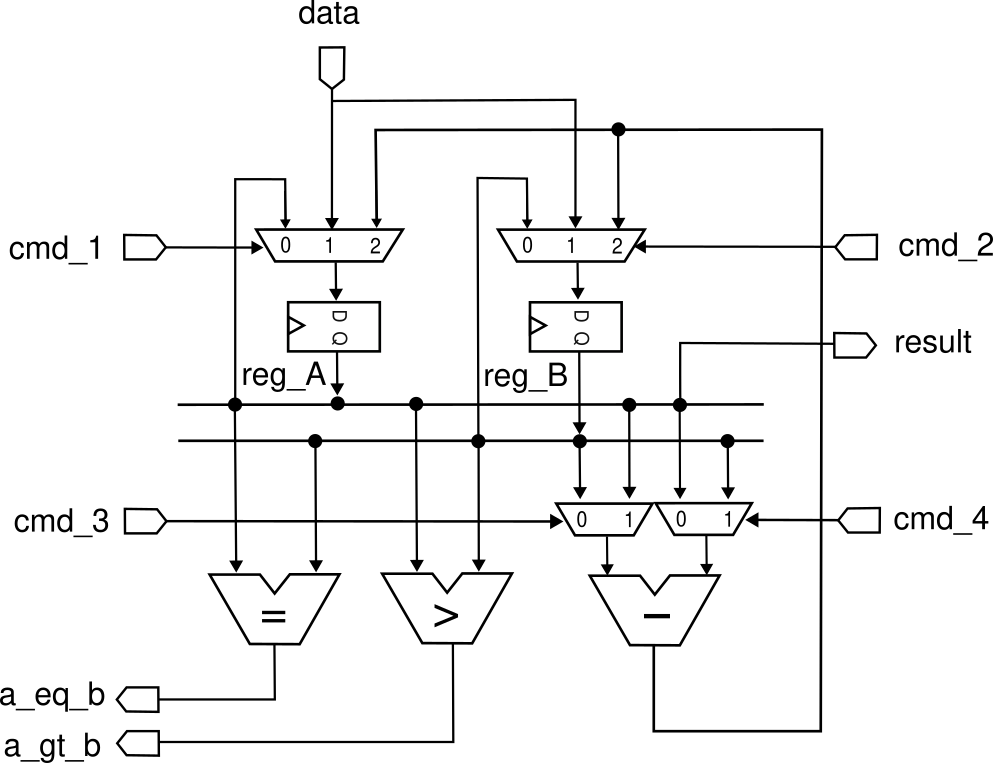
\includegraphics[scale=0.28]{./images/gcd_0}
      \end{center}
    \end{column}
  \end{columns}
\end{frame}

\begin{frame}{FSMD : exemple \texttt{GCD} (Euclide)}
  \begin{center}
    \fbox{\textbf{Contrôleur (FSM)} : Quelle séquence ? Quelles prises de décision ? Quelles actions sur le \textit{datapath} ?}
  \end{center}
  \begin{columns}
    \begin{column}{0.40\textwidth}
      \begin{block}{Pseudo-code}
          \begin{algorithmic}[1]
              \State $reg_a \gets \text{read}(data)$
              \State $reg_b \gets \text{read}(data)$
              \While{$reg_a \neq reg_b$}
                  \If{$reg_a > reg_b$}
                      \State $reg_a \gets reg_a - reg_b$
                  \Else
                      \State $reg_b \gets reg_b - reg_a$
                  \EndIf
              \EndWhile
              \State \Return $reg_a$
          \end{algorithmic}
      \end{block}
    \end{column}
    \begin{column}{0.50\textwidth}
      \begin{center}
        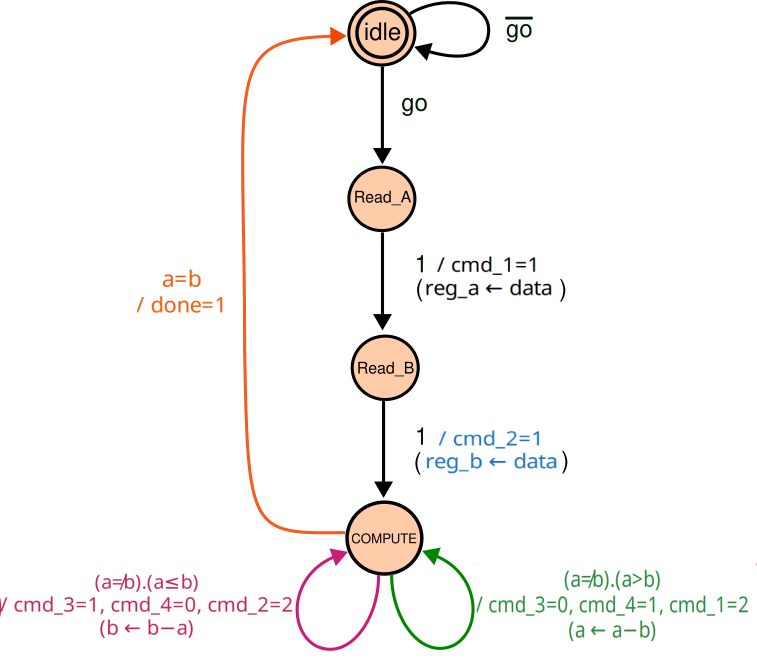
\includegraphics[scale=0.32]{./images/gcd_fsm}
      \end{center}
    \end{column}
  \end{columns}
\end{frame}

\begin{frame}{FSMD \texttt{GCD} : Assemblage FSMD}
  \begin{columns}
    \begin{column}{0.40\textwidth}
      \begin{center}
        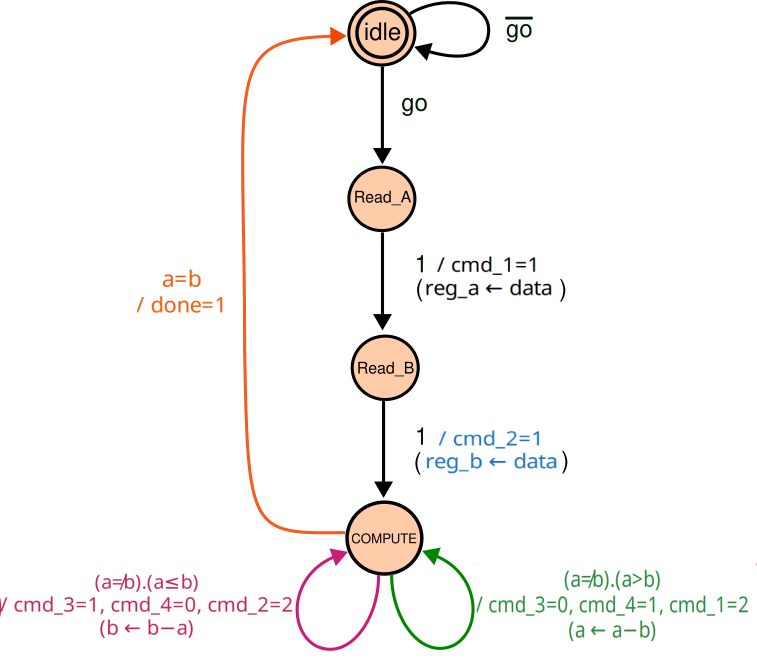
\includegraphics[scale=0.32]{./images/gcd_fsm}
      \end{center}
    \end{column}
    \begin{column}{0.50\textwidth}
      \begin{center}
        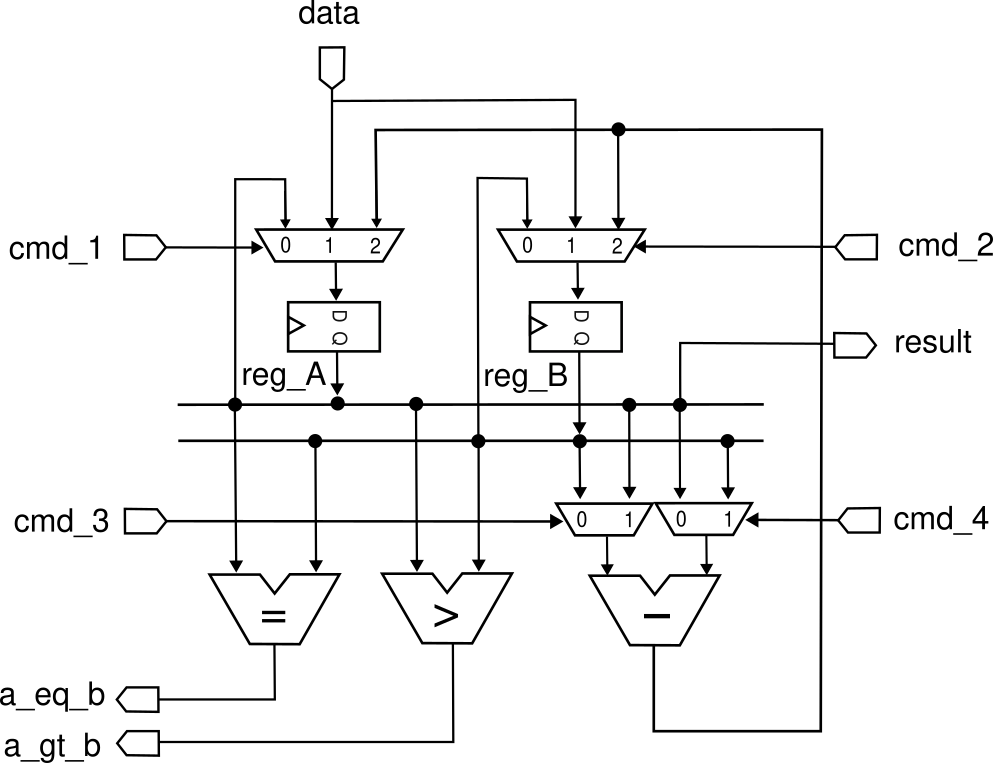
\includegraphics[scale=0.3]{./images/gcd_0}
      \end{center}
    \end{column}
  \end{columns}
\end{frame}

\begin{frame}[t]{Séquencement de $\mathrm{pgcd}(48,18)$ : }
  \centering
  \footnotesize
  \setlength{\tabcolsep}{5pt}
  \renewcommand{\arraystretch}{1.2}
  \begin{tabular}{@{}r l r c c c c r r l@{}}
    \toprule
    \textbf{Cycle} & \textbf{État} & \texttt{data} &
    \texttt{cmd\_1} & \texttt{cmd\_2} & \texttt{cmd\_3} & \texttt{cmd\_4} &
    \texttt{reg\_a} & \texttt{reg\_b} & \textbf{Action du datapath} \\
    \midrule
    0 & IDLE & -- & 0 & 0 & \textcolor{gray}{0} & \textcolor{gray}{0} & 0 & 0 & \texttt{go}=1 échantillonné \\
    1 & READ\_A & 48 & \cellcolor{hl}\textbf{1} & 0 & \textcolor{gray}{0} & \textcolor{gray}{0} & 0 & 0 & \texttt{reg\_a} $\leftarrow$ \texttt{data} \\
    2 & READ\_B & 18 & 0 & \cellcolor{hl}\textbf{1} & \textcolor{gray}{0} & \textcolor{gray}{0} & 48 & 0 & \texttt{reg\_b} $\leftarrow$ \texttt{data} \\
    3 & COMPUTE & -- & \cellcolor{hl}\textbf{2} & 0 & \cellcolor{hl}\textbf{0} & \cellcolor{hl}\textbf{1} & 48 & 18 & $a>b$ : $a \leftarrow a-b$ \\
    4 & COMPUTE & -- & \cellcolor{hl}\textbf{2} & 0 & \cellcolor{hl}\textbf{0} & \cellcolor{hl}\textbf{1} & 30 & 18 & $a>b$ : $a \leftarrow a-b$ \\
    5 & COMPUTE & -- & 0 & \cellcolor{hl}\textbf{2} & \cellcolor{hl}\textbf{1} & \cellcolor{hl}\textbf{0} & 12 & 18 & $a<b$ : $b \leftarrow b-a$ \\
    6 & COMPUTE & -- & \cellcolor{hl}\textbf{2} & 0 & \cellcolor{hl}\textbf{0} & \cellcolor{hl}\textbf{1} & 12 & 6 & $a>b$ : $a \leftarrow a-b$ \\
    7 & COMPUTE & -- & 0 & 0 & \textcolor{gray}{0} & \textcolor{gray}{0} & 6 & 6 & $a=b$ $\Rightarrow$ \texttt{done}=1 \\
    \bottomrule
  \end{tabular}

  \vspace{0.8em}
  \begin{minipage}{0.96\linewidth}
    \scriptsize
    \textbf{Lecture.}
    \texttt{cmd\_1}, \texttt{cmd\_2} : 0 = conserver, 1 = charger \texttt{data}, 2 = charger \texttt{computed\_value}.
    \texttt{cmd\_3}, \texttt{cmd\_4} : sélection des opérandes (0 = \texttt{reg\_a}, 1 = \texttt{reg\_b}), \texttt{computed\_value} = \texttt{arg\_1}$-$\texttt{arg\_2}.\\
    Les commandes sont décidées et appliquées dans le même cycle ; \texttt{reg\_x} est mis à jour au front de fin de cycle.
    \texttt{reg\_a} et \texttt{reg\_b} : valeurs au début du cycle. Une itération par cycle, \texttt{done} au cycle 7.
  \end{minipage}

\end{frame}

\begin{frame}{FSMD \texttt{GCD} : remarques}
  \textbf{Plusieurs remarques:}
  \begin{enumerate}
    \item Le choix retenu ici a été la \textbf{simplicité}.
    \begin{itemize}
      \item ...au détriment de la \textit{fréquence} de fonctionnement.
      \item Notamment, le \textit{chemin critique} est \textit{assez} long :
        \begin{itemize}
          \item Logique combinatoire FSM $\Rightarrow$ logique combinatoire sélection datapath.
        \end{itemize}
    \end{itemize}
   \item Ce chemin peut être réduit par des schémas d'interposition de registres entre FSM et datapath.
   \item Mais la mise au point est plus complexe :
     \begin{itemize}
      \item Actions déclanchées à un \textbf{cycle donné}...
      \item ...dont les effets s'effectuent au \textbf{cycle suivant}.
    \end{itemize}
    \item Pipelining complexe
    \begin{itemize}
      \item Peut nécessiter des \textbf{anticipations} (\texttt{forwarding})
      \item etc
    \end{itemize}
    \item \textbf{Note :} toute la démarche implique l'existence d'un \textit{protocole} d'utilisation du circuit. Notamment l'ordre de présentation des données devra être connu au moment de la conception et respecté au moment de l'utilisation.
    %\item Le PGCD ne présente pas de \textbf{dépendances de données} complexes (voir dernier TD).
  \end{enumerate}
\end{frame}

% \section{Implémentation \texttt{VHDL} du \texttt{GCD}}
% =====================================================================
\begin{frame}[fragile,t]{FSMD : interconnexion contrôleur / chemin de données}
\begin{columns}[T]
\begin{column}{0.54\textwidth}
\codecap{fsmd.vhd}
\begin{lstlisting}
entity fsmd is
  ...
end entity;
architecture rtl of fsmd is
  signal |controls_s| : control_type;
  signal |status_s| : status_type;
begin
  controler_i: entity gcd_lib.controler
  port map (
    ...
    go       => go,
    done     => done,
    controls => |controls_s|,
    status   => |status_s|
  );
  datapath_i: entity gcd_lib.datapath
  port map (
    ...
    data     => data,
    result   => result,
    controls => |controls_s|,
    status   => |status_s|
  );
end rtl;
\end{lstlisting}
\end{column}
\begin{column}{0.44\textwidth}
\fig[62mm]{fig1_fsmd}
\end{column}
\end{columns}
\takeaway{Pur câblage structurel (aucune logique dans \texttt{fsmd}) ; deux types enregistrement de \texttt{type\_pkg} servent d'interface.}
\end{frame}

% =====================================================================
\begin{frame}[fragile,t]{Un registre du chemin de données : \texttt{reg\_a}}
\begin{columns}[T]
\begin{column}{0.54\textwidth}
\codecap{datapath.vhd}
\begin{lstlisting}
constant READ_DATA : integer range 0 to 2 := 1;
constant SAMPLE_COMPUTED_VALUE : integer range 0 to 2 := 2;
signal reg_a,reg_b, computed_value : unsigned(31 downto 0);
...
reg_a_p : process(reset_n,clk)
begin
  if reset_n='0' then
    reg_a <= to_unsigned(0,32);
  elsif rising_edge(clk) then
    case |controls.cmd_1| is
      when READ_DATA =>
        reg_a <= |data|;
      when SAMPLE_COMPUTED_VALUE =>
        reg_a <= |computed_value|;
      when others =>
        null;   -- maintien
    end case;
  end if;
end process;
...
result <= reg_a;
\end{lstlisting}
\end{column}
\begin{column}{0.44\textwidth}
\fig[62mm]{fig2_reg_a}
\end{column}
\end{columns}
\takeaway{3 comportements pilotés par \texttt{cmd\_1} : maintenir, lire \texttt{data}, échantillonner le résultat ; \texttt{reg\_b} est identique avec \texttt{cmd\_2}.}
\end{frame}

% =====================================================================
\begin{frame}[fragile,t]{Cœur de calcul : conditions et soustraction}
\begin{columns}[T]
\begin{column}{0.50\textwidth}
\codecap{datapath.vhd}
\begin{lstlisting}
arg_1 <= reg_a when |controls.cmd_3|=0 else reg_b;
arg_2 <= reg_a when |controls.cmd_4|=0 else reg_b;
computed_value <= arg_1 - arg_2;
status.a_gt_b  <= reg_a > reg_b ;
status.a_neq_b <= reg_a /= reg_b ;
\end{lstlisting}
\vspace{1.5mm}
\codecap{controler.vhd}
\begin{lstlisting}
when COMPUTE =>
  if |status.a_neq_b| then
    if |status.a_gt_b| then
      controls_c.cmd_3 <= 0;--arg1=a
      controls_c.cmd_4 <= 1;--arg2=b
      controls_c.cmd_1 <= 2;--sample result
    else
      controls_c.cmd_3 <= 1;--arg1=b
      controls_c.cmd_4 <= 0;--arg2=a
      controls_c.cmd_2 <= 2;--sample result
    end if;
  else
    done_c <= '1';
    state_c <= IDLE;
  end if;
\end{lstlisting}
\end{column}
\begin{column}{0.48\textwidth}
\fig[62mm]{fig3_calcul}
\end{column}
\end{columns}
\takeaway{Euclide par soustractions : $a>b \Rightarrow a\leftarrow a-b$, $a<b \Rightarrow b\leftarrow b-a$, $a=b \Rightarrow$ \texttt{done}.}
\end{frame}

% =====================================================================
\begin{frame}[fragile,t]{Protocole d'utilisation : \texttt{go}, puis \texttt{a} et \texttt{b} sur \texttt{data}}
  \begin{columns}[T]
    \begin{column}{0.40\textwidth}
      \codecap{fsmd\_tb.vhd}
      \begin{lstlisting}
      toggle(go);  -- impulsion de 1 cycle
      data <= to_unsigned(48,32);  -- a
      wait_cycles(1);
      data <= to_unsigned(18,32);  -- b
      wait_cycles(200);
      \end{lstlisting}
      \vspace{1.5mm}
      \codecap{controler.vhd}
      \begin{lstlisting}
      when IDLE =>
        if go='1' then
          state_c <= READ_A;
        end if;
      when READ_A =>
        controls_c.cmd_1 <= 1;  -- reg_a <= data
        state_c <= READ_B;
      when READ_B =>
        controls_c.cmd_2 <= 1;  -- reg_b <= data
        state_c <= COMPUTE;
      \end{lstlisting}
      \vspace{1.5mm}

      {\footnotesize
      \begin{enumerate}\setlength\itemsep{0pt}
        \item \texttt{go} à 1 pendant un cycle
        \item \texttt{a} sur \texttt{data} (\texttt{READ\_A})
        \item \texttt{b} sur \texttt{data} (\texttt{READ\_B})
        \item attendre \texttt{done} ; lire \texttt{result}
      \end{enumerate}}

    \end{column}

    \begin{column}{0.58\textwidth}
      \fig[62mm]{fig4_chrono}
    \end{column}
  \end{columns}
\end{frame}

% =====================================================================
\begin{frame}[fragile,t]{Architecture du banc de test}
  \begin{columns}[T]
    \begin{column}{0.54\textwidth}
    \codecap{fsmd\_tb.vhd}
    \begin{lstlisting}
    entity fsmd_tb is
    end entity;
    architecture bhv of fsmd_tb is
      constant HALF_PERIOD : time :=5 ns;
      signal clk : std_logic := '0';
      signal running : boolean := true;
      procedure wait_cycles(n : natural) is ...
      procedure toggle(signal s : inout std_logic) is ...
      ...
    begin
      |reset_n| <= '0','1' after 123 ns;
      |clk| <= not(clk) after HALF_PERIOD when running else clk;
      |dut| : entity work.fsmd(rtl)
        port map (
          ...
        );
      |stim| : process
      begin
        wait until reset_n='1';
        ...
        running <= false;
        wait;
      end process;
    end bhv;
    \end{lstlisting}
    \end{column}

    \begin{column}{0.44\textwidth}
      \fig[62mm]{fig5_testbench}
    \end{column}
  \end{columns}
  \takeaway{Testbench sans port : horloge, reset, DUT et processus de stimuli ; pas d'\texttt{assert}, on vérifie \texttt{result} (= 6) au chronogramme.}
\end{frame}

\begin{frame}{Résultats de simulation VHDL}
  \begin{center}
    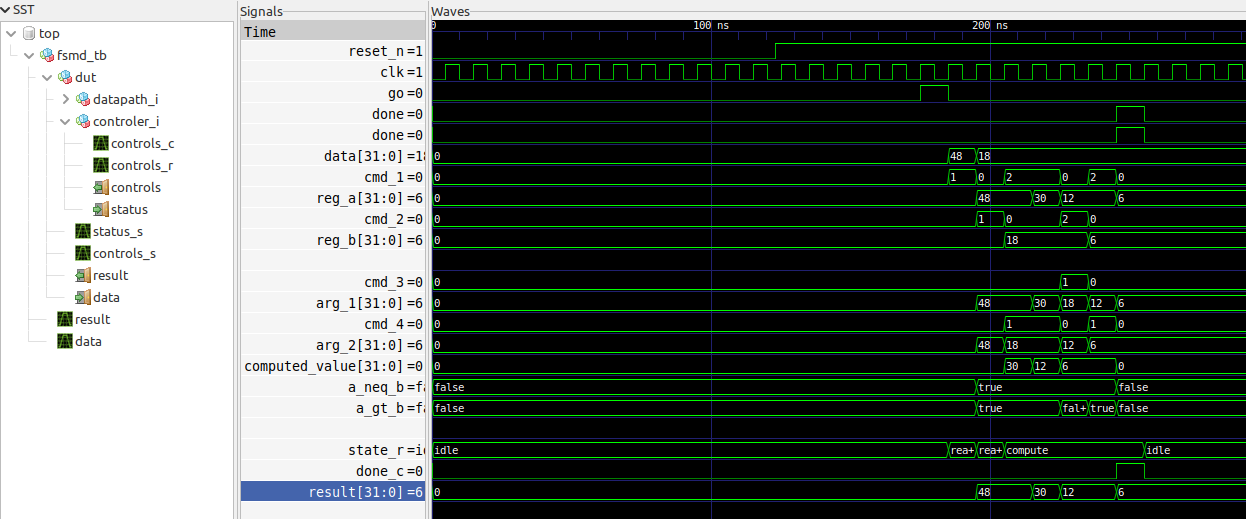
\includegraphics[scale=0.3]{./images/gcd_gtkwave.png}
  \end{center}
\end{frame}

\begin{frame}[fragile,t]{Script de simulation :  GHDL + GTKWave}
  \begin{columns}[T]
    \begin{column}{0.52\textwidth}
    \codecap{compile.x}
    \begin{lstlisting}[style=shell]
    echo "=> cleaning"
    rm *.cf

    echo "=> compiling RTL files"
    ghdl @-a@ --work=gcd_lib type_pkg.vhd
    ghdl @-a@ --work=gcd_lib controler.vhd
    ghdl @-a@ --work=gcd_lib datapath.vhd
    ghdl @-a@ --work=gcd_lib fsmd.vhd

    echo "=> compiling testbench"
    ghdl @-a@ --work=gcd_lib fsmd_tb.vhd

    echo "=> elaboration"
    ghdl @-e@ --work=gcd_lib fsmd_tb

    echo "=> running simulation"
    ghdl @-r@ --work=gcd_lib fsmd_tb --wave=top.ghw

    echo "=> opening waveform viewer"
    gtkwave top.ghw top.sav
    \end{lstlisting}
    \end{column}

    \begin{column}{0.46\textwidth}
      \fig[64mm]{fig6_compile}
    \end{column}
  \end{columns}
  \takeaway{Tout est compilé dans la bibliothèque \texttt{gcd\_lib} (\texttt{-{}-work}) : \texttt{type\_pkg} d'abord, \texttt{fsmd} après ses deux sous-blocs.}
\end{frame}

%========================================================================================
%                               mémoires et processeurs
%========================================================================================
\section{Mémoires SRAM et DRAM}
% ==============================================================================
% FRAME 1 : SRAM
% ==============================================================================

\begin{frame}{Stockage des données \textit{massives}}
  \begin{columns}[T]
    \begin{column}{0.5\textwidth}
      \begin{itemize}
        \item Les \textbf{registres} stockent les données.
        \begin{itemize}
          \item \textbf{Rappel} : \textit{registre} =  \textit{Bascule D}.
        \end{itemize}
        \item Mais ils ont un coût élevé :
        \begin{itemize}
          \item Environ 10 portes logiques pour 1 bascule D.
          \item Prohibitif pour de grandes qualité de données.
          \item Nécessité d'autres technologies pour ce stockage massif.
        \end{itemize}
        \item Objectif : se rapprocher de la manipulation logicielle de \textit{tableaux}
          \begin{itemize}
            \item \texttt{int t[1000]=\{23,18,5,-4,...\};}
            \item \texttt{t[123] = -47; // écriture}
            \item \texttt{int x= 42 * t[2]; // lecture}
          \end{itemize}
        \end{itemize}
    \end{column}
    \begin{column}{0.5\textwidth}
      \centering
      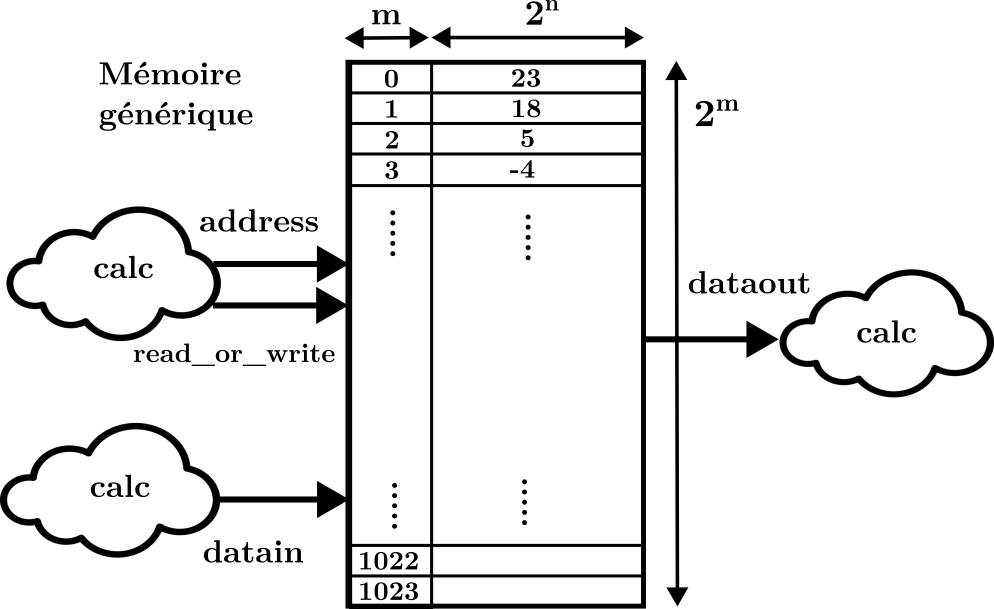
\includegraphics[scale=0.29]{./images/memory.png}
    \end{column}
  \end{columns}
\end{frame}

\begin{frame}{Mémoire SRAM (Static Random Access Memory)}
  \small
    \begin{columns}[T]
        \begin{column}{0.55\textwidth}
            \textbf{Principe de la cellule (6T)} :
            \begin{itemize}
                \item Bistable à 6 transistors (2 inverseurs couplés + 2 transistors d'accès).
                \item \textbf{Statique} : conserve l'information tant qu'elle est alimentée (pas de rafraîchissement).
                \item Très rapide, mais faible densité (surface silicium importante).
            \end{itemize}

            \vspace{0.3cm}
            \textbf{Signaux de commande typiques} :
            \begin{itemize}
                \item \texttt{ADDR} : Bus d'adresse (sélectionne la ligne via \textit{Word Line} et la colonne).
                \item \texttt{CS} (\textit{Chip Select}) : Activation de la puce.
                \item \texttt{WE} (\textit{Write Enable}) : \texttt{1} pour écriture, \texttt{0} pour lecture.
                \item \texttt{OE} (\textit{Output Enable}) : Active les buffers de sortie.
                \item \texttt{D\textsubscript{in}} / \texttt{D\textsubscript{out}} : Bus de données.
            \end{itemize}
        \end{column}

        \begin{column}{0.45\textwidth}
            \centering
            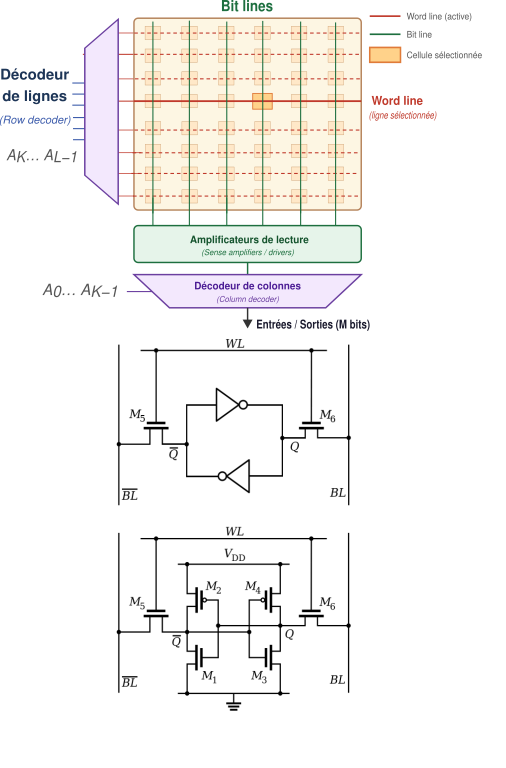
\includegraphics[scale=0.39]{./images/sram_cellule_6t.png}
        \end{column}
    \end{columns}
\end{frame}

% ==============================================================================
% FRAME 2 : DRAM
% ==============================================================================
\begin{frame}{Mémoire DRAM (Dynamic Random Access Memory)}
    \small
    \begin{columns}[T]
        \begin{column}{0.55\textwidth}
            \textbf{Principe de la cellule (1T1C)} :
            \begin{itemize}
                \item 1 Transistor d'accès + 1 Condensateur de stockage.
                \item \textbf{Dynamique} : la charge du condensateur fuit, nécessitant un \textbf{rafraîchissement périodique} (typ. toutes les 64 ms).
                \item Haute densité, faible coût par bit, mais lente.
            \end{itemize}

            \vspace{0.3cm}
            \textbf{Signaux de commande et usage} :
            \begin{itemize}
                \item \texttt{RAS} (\textit{Row Address Strobe})
                \begin{itemize}
                  \item Valide l'adresse de ligne (ouvre la rangée).
                \end{itemize}
                \item \texttt{CAS} (\textit{Column Address Strobe}) :
                \begin{itemize}
                  \item Valide l'adresse de colonne (sélectionne le mot).
                \end{itemize}
                \item \texttt{WE} : \texttt{0} pour écriture, \texttt{1} pour lecture (e.g).
                \item \texttt{DQ} : Bus de données bidirectionnel (Data In/Out multiplexé).
            \end{itemize}
        \end{column}

        \begin{column}{0.45\textwidth}
            \centering
            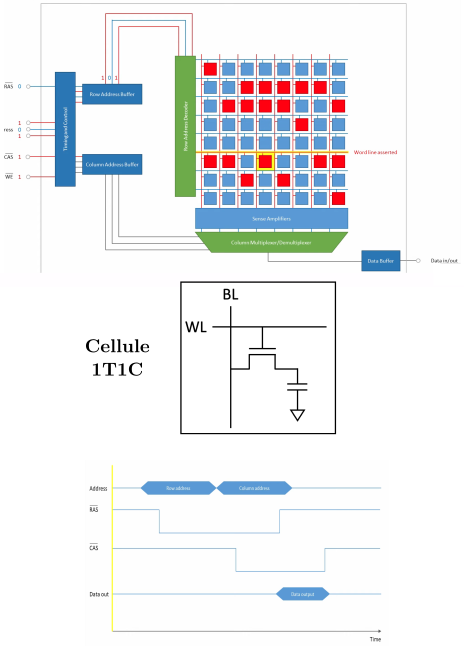
\includegraphics[scale=0.45]{./images/dram_cellule_1t1c.png}
        \end{column}
    \end{columns}
\end{frame}

% ==============================================================================
% FRAME 3 : COMPARAISON ET HIÉRARCHIE
% ==============================================================================
\begin{frame}{Comparaison et Utilisation dans la Hiérarchie Mémoire}
    \small
    \begin{table}
      \centering
      \renewcommand{\arraystretch}{1.3}
      \begin{tabular}{lcc}
        \toprule
        \textbf{Caractéristique} & \textbf{SRAM} & \textbf{DRAM} \\
        \midrule
        \textbf{Cellule} & 6 transistors (6T) & 1T + 1 Condensateur (1T1C) \\
        \textbf{Densité} & Faible & Élevée \\
        \textbf{Vitesse d'accès} & Très rapide (\(\sim\) 1-10 ns) & Rapide (\(\sim\) 10-50 ns) \\
        \textbf{Rafraîchissement} & Non requis & Obligatoire (périodique) \\
        \textbf{Consommation} & Faible (en veille) & Moyenne (à cause du refresh) \\
        \textbf{Coût par bit} & Élevé & Faible \\
        \bottomrule
      \end{tabular}
    \end{table}

    \begin{columns}[T]
        \begin{column}{0.6\textwidth}
            \vspace{0.2cm}
            \textbf{Utilisation système typique} :
            \begin{itemize}
                \item \textbf{SRAM} : Mémoires Cache (L1, L2, L3), mémoires tampons, registres. Proche du cœur de processeur.
                \item \textbf{DRAM} : Mémoire principale du système (barrettes DDR4/DDR5). Gestion par un contrôleur mémoire dédié (MMC).
            \end{itemize}
        \end{column}

        \begin{column}{0.4\textwidth}
            \centering
            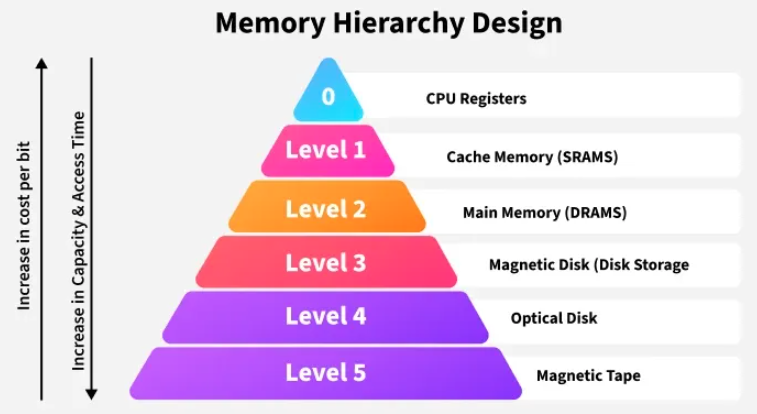
\includegraphics[scale=0.22]{./images/memory_hierarchy.png}
        \end{column}
    \end{columns}
\end{frame}

\section{Des FSMD aux Microprocesseurs}

%====================================================================
\begin{frame}{1. Rappel : la FSMD, un algorithme câblé}
\begin{columns}[T]
\begin{column}{0.50\textwidth}
\centering
\begin{tikzpicture}[font=\scriptsize,>=Stealth]
  \node[st] (s0) at (0,1.5) {$S_0$};
  \node[st] (s1) at (2.2,1.5) {$S_1$};
  \node[st] (s2) at (4.4,2.7) {$S_2$};
  \node[st] (s3) at (4.4,0.3) {$S_3$};
  \draw[<-,thick] (s0.west) -- ++(-0.6,0) node[left,lab]{reset};
  \draw[->,thick] (s0) -- (s1);
  \draw[->,thick] (s1) to[bend left=20] node[above,sloped,lab]{$R_2\neq 0$} (s2);
  \draw[->,thick] (s2) to[bend left=20] (s1);
  \draw[->,thick] (s1) -- node[below,sloped,lab]{$R_2=0$} (s3);
  \path[->,thick] (s3) edge[loop right] (s3);
\end{tikzpicture}

\vspace{2mm}
\footnotesize Calcul de $Y = A \times B$ par additions successives (registres $R_1,R_2,R_3$).
\end{column}
\begin{column}{0.50\textwidth}
\scriptsize
\renewcommand{\arraystretch}{1.3}
\begin{tabular}{|c|l|}
\hline
\rowcolor{\cS} $S_0$ & $R_1 \aff A$ ;\; $R_2 \aff B$ ;\; $R_3 \aff 0$ \\ \hline
\rowcolor{\cT} $S_1$ & si $R_2 = 0$ alors $S_3$ sinon $S_2$ \\ \hline
\rowcolor{\cU} $S_2$ & $R_3 \aff R_3 + R_1$ ;\; $R_2 \aff R_2 - 1$ ;\; $\to S_1$ \\ \hline
\rowcolor{\cV} $S_3$ & $Y \aff R_3$ ;\; fin \\ \hline
\end{tabular}
\end{column}
\end{columns}

\vspace{3mm}
\begin{block}{Ce qu'il faut remarquer}
\footnotesize
\begin{itemize}\setlength{\itemsep}{1pt}
 \item Le \alert{séquencement} (graphe d'états) \emph{est} l'algorithme : changer d'algorithme $=$ refaire la FSM.
 \item Les registres $R_i$ sont \alert{nommés} dans les actions et \alert{câblés} à l'UAL.
 \item Une action d'état peut faire \alert{plusieurs transferts en parallèle} ($S_2$).
\end{itemize}
\end{block}
\end{frame}

%====================================================================
\begin{frame}{2. L'idée : extraire le programme de la FSM}
  \begin{center}
    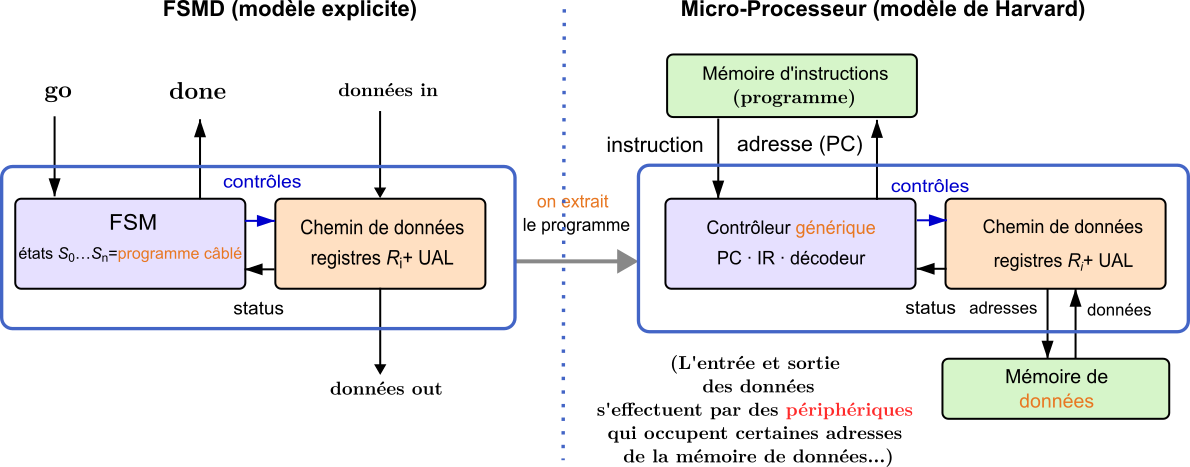
\includegraphics[scale=0.4]{./images/fsmd_proc.png}
  \end{center}

  \vspace{2mm}
  \begin{block}{Idée directrice}
  \footnotesize
  Si le séquencement est \emph{lu} dans une mémoire au lieu d'être câblé, la FSM devient générique (la même pour tout programme) :
  on obtient un \alert{processeur}. Le programme devient une \alert{donnée}.
  \end{block}
\end{frame}

%====================================================================
\begin{frame}{3. La mémoire de données et registres de travail}
  \begin{columns}[T]
    \begin{column}{0.44\textwidth}
      \footnotesize
      \textbf{Dans la FSMD} : quelques registres $R_i$, câblés à l'UAL, désignés \emph{par leur nom} dans les actions d'état.

      \medskip
      \textbf{Limite} : le nombre de registres est petit (coût en surface, en multiplexeurs).

      \medskip
      \textbf{Extension naturelle} :
      \begin{itemize}\setlength{\itemsep}{1pt}
        \item un \alert{banc de registres} : registres désignés par un \emph{numéro} (champ de l'instruction) ;
        \item une \alert{mémoire de données} : beaucoup de mots, désignés par une \emph{adresse}, mais \alert{non reliée directement à l'UAL}.
      \end{itemize}

      \medskip
      Deux instructions de transfert suffisent : \texttt{LD} (mémoire $\to$ registre) et \texttt{ST} (registre $\to$ mémoire).
    \end{column}

    \begin{column}{0.56\textwidth}
      \centering
      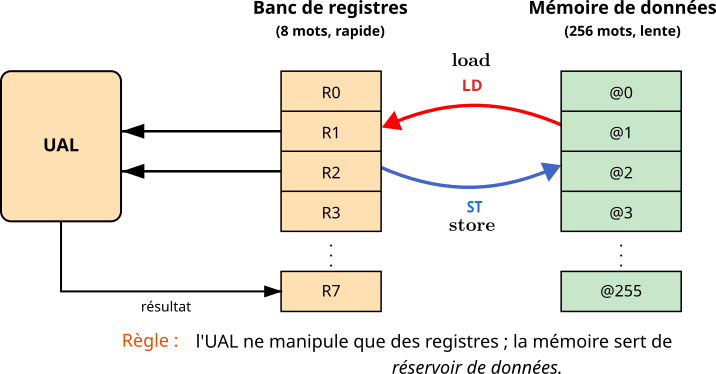
\includegraphics[scale=0.4]{./images/reg_mem.png}
    \end{column}
  \end{columns}

  \begin{block}{A retenir}
  \footnotesize
  On parle d'\textit{"architecture \texttt{load-store}""}
  \end{block}
\end{frame}

%====================================================================
\begin{frame}{4. Architecture de Harvard : deux mémoires, un contrôleur générique}
\centering
\begin{tikzpicture}[font=\scriptsize]
  \node[box,ctrl,minimum width=1.2cm] (pc) at (0,0) {PC};
  \node[box,mem,minimum width=2.6cm] (im) at (3.4,0) {Mémoire\\d'instructions};
  \node[box,ctrl,minimum width=2.8cm] (id) at (7.4,0) {IR + décodeur\\(unité de contrôle)};
  \draw[dat] (pc) -- (im) node[midway,above,lab]{adresse};
  \draw[dat] (im) -- (id) node[midway,above,lab]{instruction};
  \draw[dat,dashed] (id.north) -- ++(0,0.6) -| (pc.north) node[pos=0.25,above,lab]{PC $\leftarrow$ PC+1, ou saut};

  \node[box,data,minimum width=2.2cm] (rf) at (2.4,-2.7) {Banc de\\registres};
  \node[box,data,minimum width=1.6cm] (alu) at (6.0,-2.7) {UAL};
  \node[box,mem,minimum width=2.4cm] (dm) at (9.6,-2.7) {Mémoire\\de données};

  \draw[cmd] (id.south) to[out=-90,in=90] (rf.north);
  \draw[cmd] (id.south) to[out=-90,in=90] (alu.north);
  \draw[cmd] (id.south) to[out=-90,in=90] node[pos=0.55,right,lab]{commandes} (dm.north);

  \draw[dat] (rf.east) -- (alu.west) node[midway,above,lab]{opérandes};
  \draw[dat] (alu.east) -- (dm.west) node[midway,above,lab]{adresse};
  \draw[dat] (alu.south) -- ++(0,-0.6) -| ([xshift=3mm]rf.south) node[pos=0.25,below,lab]{résultat};
  \draw[dat] (dm.south) -- ++(-0cm,-1.0) -| ([xshift=-3mm]rf.south) node[pos=0.25,below,lab]{LD : donnée lue};

  \node[align=left,text width=3cm,font=\footnotesize] at (11.8,0.2)
    {\alert{Harvard} : deux mémoires, deux bus $\Rightarrow$ lecture de l'instruction et accès aux données \alert{simultanés}.};
\end{tikzpicture}

\vspace{1mm}
\footnotesize
\begin{tabular}{@{}ll@{}}
\textbf{FSMD} $\to$ \textbf{processeur} : & registres $\to$ banc de registres $+$ mémoire de données ; \\
& FSM spécifique $\to$ PC $+$ IR $+$ décodeur $+$ mémoire d'instructions.
\end{tabular}
\end{frame}

%====================================================================
\begin{frame}{5. Format d'une instruction : opcode, sources, destination}
  \begin{columns}[T]
    \begin{column}{0.64\textwidth}
      \centering
      \begin{tikzpicture}[font=\scriptsize]
        \node[anchor=west,font=\scriptsize\bfseries] at (0,2.0) {Format R (registre)};
        \node[field,fill=red!20, minimum width=1.68cm,anchor=west] at (0,1.05) {opcode};
        \node[field,fill=orange!25,minimum width=1.26cm,anchor=west] at (1.68,1.05) {rd};
        \node[field,fill=blue!15, minimum width=1.26cm,anchor=west] at (2.94,1.05) {rs1};
        \node[field,fill=blue!15, minimum width=1.26cm,anchor=west] at (4.20,1.05) {rs2};
        \node[field,fill=gray!15, minimum width=1.26cm,anchor=west] at (5.46,1.05) {--};
        \node[lab,anchor=south] at (0.84,1.45) {4 bits};
        \foreach \x in {2.31,3.57,4.83,6.09} {
          \node[lab,anchor=south] at (\x,1.45) {3};
        }
        \node[lab,anchor=north] at (0.84,0.65) {\texttt{0000}};
        \node[lab,anchor=north] at (2.31,0.65) {\texttt{011}};
        \node[lab,anchor=north] at (3.57,0.65) {\texttt{011}};
        \node[lab,anchor=north] at (4.83,0.65) {\texttt{001}};
        \node[lab,anchor=north] at (6.09,0.65) {\texttt{000}};
        \node[lab,anchor=west] at (6.8,1.05) {\texttt{ADD R3,R3,R1}};

        \node[anchor=west,font=\scriptsize\bfseries] at (0,-0.25) {Format I (immédiat / mémoire / saut)};
        \node[field,fill=red!20, minimum width=1.68cm,anchor=west] at (0,-0.8) {opcode};
        \node[field,fill=orange!25,minimum width=1.26cm,anchor=west] at (1.68,-0.8) {rd};
        \node[field,fill=blue!15, minimum width=1.26cm,anchor=west] at (2.94,-0.8) {rs1};
        \node[field,fill=green!20, minimum width=2.52cm,anchor=west] at (4.20,-0.8) {imm (6 bits)};
        \node[lab,anchor=north] at (0.84,-1.2) {\texttt{0100}};
        \node[lab,anchor=north] at (2.31,-1.2) {\texttt{001}};
        \node[lab,anchor=north] at (3.57,-1.2) {\texttt{000}};
        \node[lab,anchor=north] at (5.46,-1.2) {\texttt{000000}};
        \node[lab,anchor=west] at (6.8,-0.8) {\texttt{LD R1,[R0+0]}};
      \end{tikzpicture}
    \end{column}
    \begin{column}{0.36\textwidth}
      \scriptsize
      \begin{itemize}\setlength{\itemsep}{2pt}
       \item \colorbox{red!20}{opcode} : \emph{quelle} opération $\to$ décodeur $\to$ commandes ;
       \item \colorbox{blue!15}{rs1, rs2} : numéros des registres \emph{sources} ;
       \item \colorbox{orange!25}{rd} : registre \emph{destination} ;
       \item \colorbox{green!20}{imm} : constante, déplacement ou offset de saut.
      \end{itemize}
    \end{column}
  \end{columns}

  \vspace{2mm}

  \begin{block}{Mot de 16 bits}
    \footnotesize
    \texttt{ADD R3,R3,R1} $=$ \texttt{0000 0110 1100 1000} $=$ \texttt{0x06C8} \qquad
    \texttt{LD R1,[R0+0]} $=$ \texttt{0100 0010 0000 0000} $=$ \texttt{0x4200}

    \smallskip
    Une instruction n'est \alert{qu'un mot} stocké dans la mémoire d'instructions : le \og programme \fg{} est une liste de mots.
  \end{block}
\end{frame}

%====================================================================
\begin{frame}{6. Un jeu d'instructions minimal}
  \centering\footnotesize
  \renewcommand{\arraystretch}{1.25}
  \setlength{\tabcolsep}{5pt}
  \begin{tabular}{|l|l|c|c|l|}
    \hline
    \textbf{Classe} & \textbf{Instruction} & \textbf{Format} & \textbf{opcode} & \textbf{Effet (transfert de registres)} \\ \hline
    \rowcolor{\cU} Arithmétique & \texttt{ADD rd, rs1, rs2} & R & \texttt{0000} & $\R{rd} \aff \R{rs1} + \R{rs2}$ ;\; PC $\aff$ PC+1 \\
    \rowcolor{\cU} & \texttt{SUB rd, rs1, rs2} & R & \texttt{0001} & $\R{rd} \aff \R{rs1} - \R{rs2}$ ;\; PC $\aff$ PC+1 \\
    \rowcolor{\cU} & \texttt{ADDI rd, rs1, imm} & I & \texttt{0010} & $\R{rd} \aff \R{rs1} + \mathit{imm}$ ;\; PC $\aff$ PC+1 \\ \hline
    \rowcolor{\cS} Mémoire & \texttt{LD rd, [rs1+imm]} & I & \texttt{0100} & $\R{rd} \aff \M{\R{rs1}+\mathit{imm}}$ \\
    \rowcolor{\cS} & \texttt{ST rd, [rs1+imm]} & I & \texttt{0101} & $\M{\R{rs1}+\mathit{imm}} \aff \R{rd}$ \quad {\scriptsize(\emph{rd} lu comme source)} \\ \hline
    \rowcolor{\cT} Contrôle & \texttt{BEQ rd, rs1, imm} & I & \texttt{1000} & si $\R{rd}=\R{rs1}$ alors PC $\aff$ PC+$\mathit{imm}$ sinon PC+1 \\
    \rowcolor{\cT} & \texttt{JMP imm} & I & \texttt{1100} & PC $\aff$ $\mathit{imm}$ \\ \hline
  \end{tabular}

  \vspace{4mm}
  \begin{minipage}{0.9\textwidth}
    \footnotesize
    \begin{itemize}\setlength{\itemsep}{2pt}
       \item \texttt{R0} est câblé à $0$ : \texttt{ADDI R3,R0,0} met $R_3$ à zéro, \texttt{[R0+k]} désigne l'adresse absolue $k$.
       \item Une instruction $=$ \alert{un seul transfert} (la FSMD pouvait en faire plusieurs par état).
       \item \texttt{BEQ}/\texttt{JMP} sont les seules à modifier PC autrement que par $+1$ : ce sont les \alert{transitions} de la FSM.
    \end{itemize}
  \end{minipage}
\end{frame}

%====================================================================
\begin{frame}{7. Décodage : du mot binaire au pilotage du datapath}
  \centering
  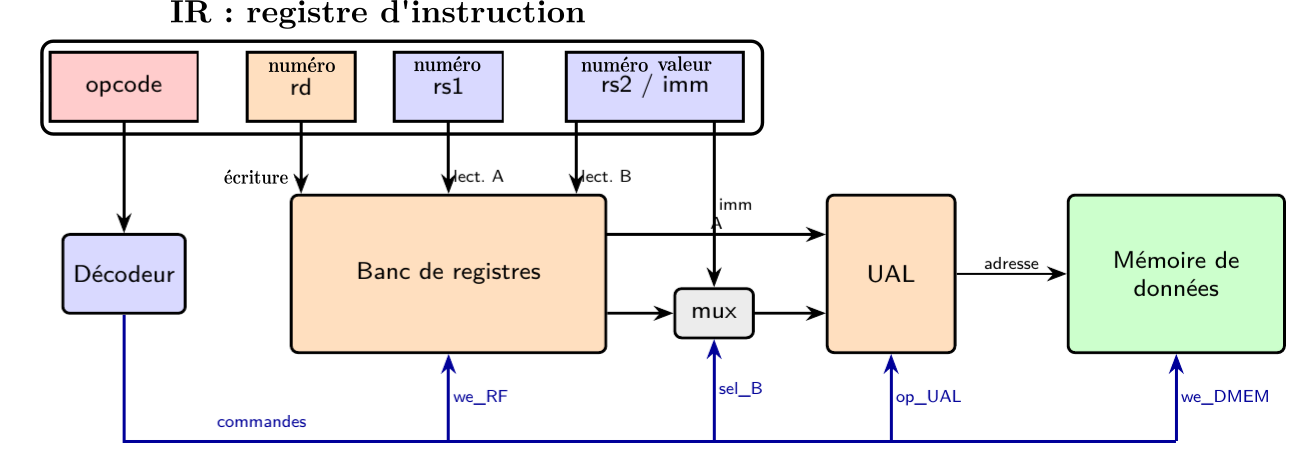
\includegraphics[scale=0.4]{./images/decodage_ir.png}
  \vspace{2mm}

  \begin{block}{Deux exemples}
    \footnotesize
    \texttt{ADD} : op\_UAL$=+$, sel\_B$=$rs2, we\_RF$=1$, we\_DMEM$=0$ \hfill
    \texttt{ST} : op\_UAL$=+$ (adresse), sel\_B$=$imm, we\_RF$=0$, we\_DMEM$=1$

    \smallskip
    Le décodeur est un circuit \alert{combinatoire} : opcode $\to$ commandes. Les numéros de registres vont \alert{directement} au banc de registres.
  \end{block}
\end{frame}

%====================================================================
\begin{frame}{8. Le cycle d'instruction : une FSM générique à la place de la FSM dédiée}
\begin{columns}[T]
  \begin{column}{0.50\textwidth}
  \centering
  \begin{tikzpicture}[font=\scriptsize,
    st/.style={circle,draw,thick,fill=blue!15,minimum size=1.5cm,align=center,inner sep=1pt}]
    \node[st] (f) at (0,0) {FETCH};
    \node[st] (d) at (2.5,0) {DECODE};
    \node[st] (e) at (5.0,0) {EXECUTE};
    \draw[dat] (f) -- (d);
    \draw[dat] (d) -- (e);
    \draw[dat] (e.south) -- ++(0,-0.5) -| (f.south);
    \node[align=center,text width=2.2cm,font=\tiny] at (0,-2.1) {IR $\aff$ IMEM[PC]\\PC $\aff$ PC+1};
    \node[align=center,text width=2.2cm,font=\tiny] at (2.5,-2.1) {lecture de rs1, rs2\\dans le banc de registres};
    \node[align=center,text width=2.4cm,font=\tiny] at (5.0,-2.1) {UAL / accès DMEM\\écriture dans rd ou PC};
  \end{tikzpicture}

  \vspace{1mm}
  \footnotesize
  Cette FSM est \alert{la même quel que soit le programme} : seul le contenu de la mémoire d'instructions change.
  \end{column}

  \begin{column}{0.45\textwidth}
    \scriptsize
    \renewcommand{\arraystretch}{1.2}
    \setlength{\tabcolsep}{3pt}
    \begin{tabular}{|p{2.5cm}|p{3.2cm}|}
    \hline
    \textbf{FSMD} & \textbf{Processeur} \\ \hline
    état $S_i$ & instruction à l'adresse PC $=i$ \\ \hline
    action $R_a \aff R_b \circ R_c$ & champs \texttt{opcode, rd, rs1, rs2} \\ \hline
    signaux de commande (câblés) & sorties du décodeur \\ \hline
    transition conditionnelle & \texttt{BEQ}, \texttt{JMP} (modifient PC) \\ \hline
    registres de travail & banc de registres $+$ mémoire de données \\ \hline
    \end{tabular}
    \end{column}
\end{columns}

\vspace{2mm}
\begin{block}{À retenir}
\footnotesize
Un processeur est une FSMD dont le \alert{séquencement est lu} en mémoire : \alert{un état $=$ une instruction}, \alert{PC $=$ registre d'état}.
\end{block}
\end{frame}

%====================================================================
\begin{frame}{9. Fil rouge : FSMD puis en programme}
\begin{columns}[T]
\begin{column}{0.44\textwidth}
\centering\footnotesize\textbf{FSMD}\par\vspace{1mm}
\scriptsize
\renewcommand{\arraystretch}{1.5}
\begin{tabular}{|c|l|}
\hline
\rowcolor{\cS} $S_0$ & $R_1 \aff A$ ;\; $R_2 \aff B$ ;\; $R_3 \aff 0$ \\ \hline
\rowcolor{\cT} $S_1$ & si $R_2 = 0$ alors $S_3$ sinon $S_2$ \\ \hline
\rowcolor{\cU} $S_2$ & $R_3 \aff R_3 + R_1$ ;\; $R_2 \aff R_2 - 1$ \\ \hline
\rowcolor{\cV} $S_3$ & $Y \aff R_3$ ;\; fin \\ \hline
\end{tabular}
\end{column}
\begin{column}{0.56\textwidth}
\centering\footnotesize\textbf{Programme} (mémoire d'instructions)\par\vspace{1mm}
\scriptsize
\renewcommand{\arraystretch}{1.1}
\begin{tabular}{|c|l|l|}
\hline
\textbf{PC} & \textbf{Instruction} & \textbf{Commentaire} \\ \hline
\rowcolor{\cS} 0 & \texttt{LD R1,[R0+0]} & $R_1 \aff A$ \\
\rowcolor{\cS} 1 & \texttt{LD R2,[R0+1]} & $R_2 \aff B$ \\
\rowcolor{\cS} 2 & \texttt{ADDI R3,R0,0} & $R_3 \aff 0$ \\ \hline
\rowcolor{\cT} 3 & \texttt{BEQ R2,R0,+4} & si $R_2=0$ aller en 7 \\ \hline
\rowcolor{\cU} 4 & \texttt{ADD R3,R3,R1} & $R_3 \aff R_3+R_1$ \\
\rowcolor{\cU} 5 & \texttt{ADDI R2,R2,-1} & $R_2 \aff R_2-1$ \\
\rowcolor{\cU} 6 & \texttt{JMP 3} & retour au test \\ \hline
\rowcolor{\cV} 7 & \texttt{ST R3,[R0+2]} & $Y \aff R_3$ \\
\rowcolor{\cV} 8 & \texttt{JMP 8} & boucle (fin) \\ \hline
\end{tabular}
\end{column}
\end{columns}

\vspace{2mm}
\begin{block}{Ce qui change}
\footnotesize
\begin{itemize}\setlength{\itemsep}{1pt}
 \item Entrées/sortie $A$, $B$, $Y$ : ce sont maintenant des \alert{cases de la mémoire de données} (@0, @1, @2).
 \item Un état à deux transferts ($S_2$) devient \alert{plusieurs instructions} : un transfert par instruction.
 \item Le graphe d'états a disparu : il est \alert{encodé dans les adresses et les sauts}.
\end{itemize}
\end{block}
\end{frame}

%====================================================================
\begin{frame}{10. Trace d'exécution pour $A=3$, $B=2$}
\centering
\scriptsize
\renewcommand{\arraystretch}{1.12}
\setlength{\tabcolsep}{5pt}
\begin{tabular}{|c|c|l|c|c|c|c|l|}
\hline
\textbf{n} & \textbf{PC} & \textbf{Instruction} & $R_1$ & $R_2$ & $R_3$ & $\M{2}$ & \textbf{Remarque} \\ \hline
1 & 0 & \texttt{LD R1,[R0+0]} & 3 & -- & -- & -- & \\
2 & 1 & \texttt{LD R2,[R0+1]} & 3 & 2 & -- & -- & \\
3 & 2 & \texttt{ADDI R3,R0,0} & 3 & 2 & 0 & -- & \\
\rowcolor{\cT} 4 & 3 & \texttt{BEQ R2,R0,+4} & 3 & 2 & 0 & -- & non pris : PC $\aff$ 4 \\
5 & 4 & \texttt{ADD R3,R3,R1} & 3 & 2 & 3 & -- & \\
6 & 5 & \texttt{ADDI R2,R2,-1} & 3 & 1 & 3 & -- & \\
7 & 6 & \texttt{JMP 3} & 3 & 1 & 3 & -- & PC $\aff$ 3 \\
\rowcolor{\cT} 8 & 3 & \texttt{BEQ R2,R0,+4} & 3 & 1 & 3 & -- & non pris \\
9 & 4 & \texttt{ADD R3,R3,R1} & 3 & 1 & 6 & -- & \\
10 & 5 & \texttt{ADDI R2,R2,-1} & 3 & 0 & 6 & -- & \\
11 & 6 & \texttt{JMP 3} & 3 & 0 & 6 & -- & \\
\rowcolor{\cT} 12 & 3 & \texttt{BEQ R2,R0,+4} & 3 & 0 & 6 & -- & \alert{pris} : PC $\aff$ 3+4 $=7$ \\
\rowcolor{\cV} 13 & 7 & \texttt{ST R3,[R0+2]} & 3 & 0 & 6 & \alert{6} & $Y = 6$ \\ \hline
\end{tabular}

\vspace{2mm}
\footnotesize
La FSMD fait la même chose en $1 + 2\times 2 + 1 + 1 = 7$ cycles ($S_0$, deux tours $S_1S_2$, $S_1$, $S_3$) ; le processeur exécute ici \alert{13 instructions} : on a échangé du \emph{temps} contre de la \emph{généralité}.
\end{frame}

%====================================================================
\begin{frame}{11. Bilan et ouverture}
\begin{columns}[T]
\begin{column}{0.5\textwidth}
\centering
\begin{tikzpicture}[font=\scriptsize]
  \node[font=\footnotesize\bfseries] at (1.8,2.4) {Harvard};
  \node[box,ctrl] (c) at (1.8,1.2) {CPU};
  \node[box,mem] (i) at (0,0) {IMEM};
  \node[box,mem] (d) at (3.6,0) {DMEM};
  \draw[dat,<->] (c) -- (i) node[midway,left,lab]{bus 1};
  \draw[dat,<->] (c) -- (d) node[midway,right,lab]{bus 2};
\end{tikzpicture}
\hspace{3mm}
\begin{tikzpicture}[font=\scriptsize]
  \node[font=\footnotesize\bfseries] at (1.0,2.4) {von Neumann};
  \node[box,ctrl] (c) at (1.0,1.2) {CPU};
  \node[box,mem,minimum width=2.2cm] (m) at (1.0,0) {MEM\\(instr. + données)};
  \draw[dat,<->] (c) -- (m) node[midway,right,lab]{bus unique};
\end{tikzpicture}
\end{column}
\begin{column}{0.5\textwidth}
\footnotesize
\textbf{Ce qu'on a ajouté} à la FSMD :
\begin{itemize}\setlength{\itemsep}{1pt}
 \item PC, mémoire d'instructions, IR, décodeur ;
 \item mémoire de données, \texttt{LD}/\texttt{ST}.
\end{itemize}
\textbf{Ce qu'on a gardé} : le chemin de données (registres + UAL) et l'idée « un état $=$ des transferts ».
\end{column}
\end{columns}

\vspace{3mm}
\begin{block}{Pour aller plus loin}
\footnotesize
\begin{itemize}\setlength{\itemsep}{2pt}
 \item \alert{von Neumann} : une seule mémoire pour code et données (plus souple, mais fetch et accès données se disputent le bus).
 \item \alert{Pipeline} : chevaucher fetch, decode et execute pour approcher une instruction par cycle.
 \item Jeux d'instructions plus riches : \texttt{CALL}/\texttt{RET}, pile, interruptions, entrées/sorties.
\end{itemize}
\end{block}
\end{frame}

%========================================================================================

\end{document}
